%%%%%%%%%%%%%%%%%%%%%%%%%%%%%%%%%%%%%%%%%%%%%%%%%%%%%%%%%%%%
%%% LIVECOMS ARTICLE TEMPLATE FOR BEST PRACTICES GUIDE
%%% ADAPTED FROM ELIFE ARTICLE TEMPLATE (8/10/2017)
%%%%%%%%%%%%%%%%%%%%%%%%%%%%%%%%%%%%%%%%%%%%%%%%%%%%%%%%%%%%
%%% PREAMBLE
\documentclass[9pt,tutorial]{livecoms}
% Use the 'onehalfspacing' option for 1.5 line spacing
% Use the 'doublespacing' option for 2.0 line spacing
% Use the 'lineno' option for adding line numbers.
% Use the 'pubversion' option for adding the citation and publication information to the document footer, when the DOI is assigned and the article is added to a live issue.
% The 'bestpractices' option for indicates that this is a best practices guide.
% Omit the bestpractices option to remove the marking as a LiveCoMS paper.
% Please note that these options may affect formatting.

\usepackage[T1]{fontenc}
\usepackage[utf8]{inputenc}
\usepackage{lmodern}
\usepackage{verbatim}
\usepackage{graphicx}
\usepackage{amsmath}
\usepackage{amssymb}
\usepackage{amsthm}
\usepackage{tabularx}
\usepackage{multirow}
\usepackage{multicol}
\usepackage{fancyvrb}
\usepackage{float}
\usepackage{listings}
\usepackage{xcolor}
\usepackage{array}
\usepackage{booktabs}
\usepackage{times}
\usepackage{subcaption}
\usepackage{mathtools}
\usepackage{menukeys}
\usepackage{microtype}
\usepackage{tcolorbox}
\usepackage{newverbs}
\usepackage[title]{appendix}
\usepackage{csquotes}

\usepackage[
    type={CC},
    modifier={by-nc-sa},
    version={4.0},
]{doclicense}

\usepackage{wrapfig}
\usepackage{geometry}

\usepackage[version=4]{mhchem}
\usepackage{siunitx}
\DeclareSIUnit\Molar{M}
\usepackage[italic]{mathastext}
\graphicspath{{figures/}}

% avoid single line at top or bottom of column
\clubpenalty1000
\widowpenalty1000
\displaywidowpenalty=1000

\definecolor{listing}{rgb}{0.95,0.95,0.95}
\definecolor{command}{rgb}{0.15,0.15,0.15}
\definecolor{download}{rgb}{0.039,0.616,0.851}
\definecolor{note}{rgb}{1,0.988,0.93}
\definecolor{note_listing}{rgb}{0.94,0.925,0.86}

\lstset{
  basicstyle=\small\color{command}, % Use default font + small size and command color
  numbers=none, % No number on the side
  frame=single, % Enable a frame
  framerule=0pt, % Invisible frame frame
  framesep=5pt, % Space between text and frame
  backgroundcolor=\color{listing}, % Set background color to listing
  xleftmargin=5pt, % Extra left margin for spacing
  xrightmargin=5pt, % Extra right margin for spacing
  columns=fullflexible, %flexible or fixed or fullflexible
}

\newtcolorbox{note}{
  %basicstyle=\small\color{command}, % Use default font + small size and command color
  colback=note, % Background color (matches listings)
  colframe=note, % Set frame color to match the background
  boxrule=0pt, % Frame thickness
  sharp corners, % Square corners
  left=5pt, % Extra left padding
  right=5pt, % Extra right padding
  top=5pt, % Extra top padding
  bottom=5pt, % Extra bottom padding
}

\DisableLigatures{encoding = *, family = *} % Deal with ligature problem when copy-pasting "fi"

\renewcommand{\floatpagefraction}{0.8} % At least 80% of a page must be used by floats
\renewcommand{\textfraction}{0.1} % At least 10% of a page must contain text

\newcommand{\lmpcmd}[1]{\hspace{0pt}\colorbox{listing}{\textcolor{command}{\small{#1}}}\hspace{0pt}} % lammps command
% \newcommand{\lmpcmd}[1]{\hspace{0pt}\colorbox{listing}{\textcolor{command}{\texttt{#1}}}\hspace{0pt}} % lammps command
\newcommand{\lmpcmdnote}[1]{\hspace{0pt}\colorbox{note_listing}{\textcolor{command}{\small{#1}}}\hspace{0pt}} % lammps command inside note
\newcommand{\flrcmd}[1]{\textcolor{command}{\texttt{#1}}} % folder in monopace
\newcommand{\flecmd}[1]{\textcolor{command}{\texttt{#1}}} % files name in monopace
\newcommand{\guicmd}[1]{\textcolor{command}{\texttt{«#1»}}} % LAMMPS-GUI commands in French quotation monopace
\newcommand{\dwlcmd}[1]{\textcolor{download}{\texttt{#1}}} % downloadable files in monopace blue

% The DisableLigatures command above turns the longer dash (--) into two dashes.
% This works around it by using \lammpsgui{} instead and making the longer dash explicit.
\newcommand{\lammpsgui}{\textsf{LAMMPS\textendash GUI}}

%%%%%%%%%%%%%%%%%%%%%%%%%%%%%%%%%%%%%%%%%%%%%%%%%%%%%%%%%%%%
%%% IMPORTANT USER CONFIGURATION
%%%%%%%%%%%%%%%%%%%%%%%%%%%%%%%%%%%%%%%%%%%%%%%%%%%%%%%%%%%%

\newcommand{\versionnumber}{1.0}  % you should update the minor version number in preprints and major version number of submissions.
% Do not add a newline in the next command, no matter how long the repository name is, as it will break the link in the PDF.
\newcommand{\githubrepository}{\url{https://github.com/lammpstutorials/lammpstutorials-article}}  %this should be the main github repository for this article

\newcommand{\filepath}{https://raw.githubusercontent.com/lammpstutorials/lammpstutorials-article/main/files/}

%%%%%%%%%%%%%%%%%%%%%%%%%%%%%%%%%%%%%%%%%%%%%%%%%%%%%%%%%%%%
%%% ARTICLE SETUP
%%%%%%%%%%%%%%%%%%%%%%%%%%%%%%%%%%%%%%%%%%%%%%%%%%%%%%%%%%%%
\title{A Set of Tutorials for the LAMMPS Simulation Package [Article v\versionnumber]}

\author[1*]{Simon Gravelle}
\affil[1]{University Grenoble Alpes, CNRS, LIPhy, Grenoble, 38000, France}
\corr{simon.gravelle@cnrs.fr}{S.G.}
\orcid{Simon Gravelle}{0000-0003-2149-6706}

\author[2]{Jacob R.~Gissinger}
\affil[2]{Stevens Institute of Technology, Hoboken, NJ 07030, USA}
\orcid{Jacob R.~Gissinger}{0000-0003-0031-044X}

\author[3]{Axel Kohlmeyer}
\affil[3]{Institute for Computational Molecular Science, Temple University, Philadelphia, PA 19122, USA}
\orcid{Axel Kohlmeyer}{0000-0001-6204-6475}

\blurb{This LiveCoMS document is maintained online on GitHub at
  \githubrepository; to provide feedback, suggestions, or help improve
  it, please visit the GitHub repository and participate via the issue
  tracker.}

%%%%%%%%%%%%%%%%%%%%%%%%%%%%%%%%%%%%%%%%%%%%%%%%%%%%%%%%%%%%
%%% PUBLICATION INFORMATION
%%% Fill out these parameters when available
%%% These are used when the "pubversion" option is invoked
%%%%%%%%%%%%%%%%%%%%%%%%%%%%%%%%%%%%%%%%%%%%%%%%%%%%%%%%%%%%
\pubDOI{10.XXXX/YYYYYYY}
\pubvolume{<volume>}
\pubissue{<issue>}
\pubyear{<year>}
\articlenum{<number>}
\datereceived{Day Month Year}
\dateaccepted{Day Month Year}

%%%%%%%%%%%%%%%%%%%%%%%%%%%%%%%%%%%%%%%%%%%%%%%%%%%%%%%%%%%%
%%% ARTICLE START
%%%%%%%%%%%%%%%%%%%%%%%%%%%%%%%%%%%%%%%%%%%%%%%%%%%%%%%%%%%%

\begin{document}

\begin{frontmatter}
\maketitle

\begin{abstract}
  The availability of open-source molecular simulation software packages
  allows scientists and engineers to focus on running and analyzing
  simulations without having to write, parallelize, and validate their
  own simulation software.  While molecular simulations thus become
  accessible to a larger audience, the ``black box'' nature of such
  software packages and wide array of options and features can make it
  challenging to use them correctly, particularly for beginners in the
  topic of MD simulations.  LAMMPS is one such versatile molecular
  simulation code, designed for modeling particle-based systems across a
  broad range of materials science and computational chemistry
  applications, including atomistic, coarse-grained, mesoscale,
  grid-free continuum, and discrete element models.  LAMMPS is capable
  of efficiently running simulations of varying sizes from small desktop
  computers to large-scale supercomputing environments.  Its flexibility
  and extensibility make it ideal for complex and extensive simulations
  of atomic and molecular systems, and beyond.  This article introduces
  a suite of tutorials designed to make learning LAMMPS more accessible
  to new users.  The first four tutorials cover the basics of running
  molecular simulations in LAMMPS with systems of varying complexities.
  The second four tutorials address more advanced molecular simulation
  techniques, specifically the use of a reactive force field, grand
  canonical Monte Carlo, enhanced sampling, and the REACTER protocol.
  In addition, we introduce \lammpsgui{}, an enhanced cross-platform
  graphical text editor specifically designed for use with LAMMPS and
  able to run LAMMPS directly on the edited input.  \lammpsgui{} is used
  as the primary tool in the tutorials to edit inputs, run LAMMPS,
  extract data, and visualize the simulated systems.
\end{abstract}

\end{frontmatter}

\section{Introduction}

Molecular Simulations (MS) can be used to model a large variety of
atomic and coarse-grained systems, including solids, fluids, polymers,
and biomolecules, as well as complex interfaces and multi-component
systems.  While various MS methods exist, Molecular Dynamics (MD) and
Monte Carlo (MC) are most commonly used.  MD is the preferred method for
obtaining the accurate dynamics of a system, as it relies on solving
Newton's equations of motion.  For systems with many degrees of freedom
or complex energy landscapes, the MC method can be a better choice than
MD because it allows for efficiently exploring a configuration space
without being confined by the accessible time scale.  MC involves
performing random changes to the system configuration that are either
accepted or rejected based on energy criteria
\cite{frenkel2023understanding, allen2017computer}.  MS allows for
measuring a broad variety of properties, including structural properties
(e.g.,~bond length distribution, coordination numbers, radial
distribution functions), thermodynamic properties (e.g.,~temperature,
pressure, volume), dynamic behaviors (e.g.,~diffusion coefficient,
viscosity), and mechanical responses (e.g.,~elastic constant, Poisson
ratio).  Some of these quantities can be directly compared with
experimental data, enabling the validation of the simulated system,
while others, available only through simulations, are often useful for
interpreting experimental data~\cite{van2008molecular}.

LAMMPS (Large-scale Atomic/Molecular Massively Parallel Simulator)
\cite{lammps_home} is a highly flexible and parallel open-source MS
tool.  Over the years, a broad variety of particle interaction models
have been implemented in LAMMPS, enabling it to model a wide range of
systems, including atomic, polymeric, biological, metallic, reactive, granular,
mesoscale, grid-free continuum, and coarse-grained systems
\cite{thompson2022lammps}.  LAMMPS can be used on a single CPU core, a
multi-socket and multi-core server, an HPC cluster, or a high-end
supercomputing system.  It can efficiently handle complex and large-scale
simulations, including hybrid MPI-OpenMP parallelization
and MPI + GPU acceleration (for a subset of its functionality).

LAMMPS requires users to write detailed input files, a task that
can be particularly challenging for new users.  Although its
documentation extensively describes all available features~\cite{lammps_docs},
navigating it can be challenging.  Much of the information may be
unnecessary for common use cases, and the detailed manual can
often feel overwhelming.  Beyond the intrinsic complexity of LAMMPS, performing accurate
MS requires several complex, system-specific decisions regarding
the physics to be modeled, such as selecting the thermodynamic
ensemble (e.g.,~micro-canonical, grand-canonical), determining the
simulation duration, and choosing the sets of parameters describing the
interactions between atoms (the so-called force field)
\cite{wong2016good, van2018validation, prasad2018best}.  While these choices are independent of the
simulation software, they may occasionally be constrained by the
features available in a given package.  The tutorials in this
article aim to flatten the learning curve and guide users in
performing accurate and reliable molecular simulations with LAMMPS.

\subsection{Scope}

This set of tutorials consists of eight tutorials arranged in order of
increasing difficulty.  The novelties associated with each tutorial are
briefly described below.

In \hyperref[lennard-jones-label]{tutorial 1}, the structure of LAMMPS
input files is illustrated through the creation of a simple atomic
Lennard-Jones fluid system.  Basic LAMMPS commands are used to set up
interactions between atoms, perform an energy minimization, and finally
run a simple MD simulation in the microcanonical (NVE) and canonical (NVT)
ensembles.

In \hyperref[carbon-nanotube-label]{tutorial 2}, a more complex system
is introduced, where atoms are connected by bonds: a small carbon
nanotube.  The use of both classical and reactive force fields (here,
OPLS-AA and AIREBO) is illustrated.  An external deformation is applied
to the CNT, and its deformation is measured.  This tutorial also
demonstrates the use of an external tool to visualize breaking bonds,
and show the possibility to import LAMMPS-generated YAML log files into
Python.

In \hyperref[all-atom-label]{tutorial 3}, two components - liquid water
(flexible three-point model) and a polymer molecule - are merged and
equilibrated.  A long-range solver is used to handle the electrostatic
interactions accurately, and the system is equilibrated in the
isothermal-isobaric (NPT) ensemble; then a stretching force is applied
to the polymer.  Through this relatively complex solvated polymer
system, the tutorial demonstrates how to use type labels to make
molecule files more generic and easier to manage~\cite{typelabel_paper}.

In \hyperref[sheared-confined-label]{tutorial 4}, an electrolyte is
confined between two walls, illustrating the specifics of simulating
systems with fluid-solid interfaces.  The tutorial uses a slightly more
complex water model than \hyperref[all-atom-label]{tutorial 3}: the
rigid four-point model TIP4P/2005~\cite{abascal2005general}.  A
non-equilibrium MD is performed by imposing shear on the fluid through
moving the walls, and the fluid velocity profile is extracted.

In \hyperref[reactive-silicon-dioxide-label]{tutorial 5}, the ReaxFF
reactive force field is used, specifically designed to simulate chemical
reactions by dynamically adjusting atomic interactions
\cite{van2001reaxff}.  ReaxFF includes charge equilibration (QEq), a
method that allows the partial charges of atoms to adjust according to
their local environment.

In \hyperref[gcmc-silica-label]{tutorial 6}, a Monte Carlo simulation in
the Grand Canonical ensemble is implemented to demonstrate how LAMMPS
can be used to simulate an open system that exchanges particles with a
reservoir.

In \hyperref[umbrella-sampling-label]{tutorial 7}, an advanced free
energy method called umbrella sampling is implemented.  By calculating
an energy barrier, this tutorial describes a protocol
for addressing energy landscapes that are difficult to sample using
classical MD or MC methods.

In \hyperref[bond-react-label]{tutorial 8}, a CNT embedded in
nylon-6,6 polymer melt is simulated.  The
REACTER protocol is used to model the polymerization of nylon, and the formation
of water molecules is tracked over time~\cite{gissinger2020reacter}.

\section{Prerequisites}

\subsection{Background knowledge}

This set of tutorials assumes no prior knowledge of the LAMMPS software
itself.  To complete the tutorials, a text editor and a suitable LAMMPS
executable are required.  We use \lammpsgui{}~\cite{lammps_gui_docs}
here, as it offers features that make it particularly convenient for
tutorials, but other console or graphical text editors, such as GNU
nano, vi/vim, Emacs, Notepad, Gedit, and Visual Studio Code can also be
used.  LAMMPS can be executed either directly from \lammpsgui{}
(\hyperref[using-lammps-gui-label]{Appendix~\ref{using-lammps-gui-label}})
or from a command prompt
(\hyperref[command-line-label]{Appendix~\ref{command-line-label}}), the
latter of which requires some familiarity with executing commands from a
terminal or command-line prompt.

In addition, prior knowledge of the theoretical basics of molecular
simulations and statistical physics is highly beneficial.  Users may
refer to textbooks such as \textit{Understanding Molecular Simulation} by
Daan Frenkel and Berend Smit~\cite{frenkel2023understanding}, as well as
\textit{Computer Simulation of Liquids} by Michael Allen and Dominic
Tildesley~\cite{allen2017computer}.  To better understand
the fundamental concepts behind the soft matter systems simulated in these
tutorials, users can also refer to \textit{Basic Concepts for Simple and
  Complex Liquids} by Jean-Louis Barrat and Jean-Pierre Hansen
\cite{barrat2003basic}, as well as \textit{Theory of Simple Liquids:
  with Applications to Soft Matter} by Jean-Pierre Hansen and Ian Ranald
McDonald~\cite{hansen2013theory}.  For more resources, the SklogWiki
platform provies a wide range of information information on statistical mechanics
and molecular simulations~\cite{sklogwiki_main_page}.

\subsection{Software/system requirements}

The LAMMPS stable release version 29Aug2024\_update2~\cite{lammps_code}
and the matching \lammpsgui{} software version 1.6.12 are required to
follow the tutorials, as they include features that were first
introduced in these versions.  For Linux (x86\_64 CPU), macOS (BigSur or
later), and Windows (10 and 11) you can download a precompiled LAMMPS
package from the LAMMPS release page on
GitHub~\cite{lammps_github_release}.  Select a package with `GUI' in the
file name, which includes both, \lammpsgui{} and the LAMMPS command-line
executable.  These precompiled packages are designed to be portable, and
therefore omit support for parallel execution with MPI.  Instructions
for installing \lammpsgui{} and using its most relevant features for the
tutorials are provided in
\hyperref[using-lammps-gui-label]{Appendix~\ref{using-lammps-gui-label}}.

LAMMPS versions are generally backward compatible, meaning that old
input files typically work with newer versions of LAMMPS.  However,
forward compatibility is not as strong, so input files written for a
newer version may not always work with an older versions.  As a result,
it is usually possible to follow this tutorial with more recent releases
of \lammpsgui{} and LAMMPS; older versions may require some (minor)
adjustments.  These tutorials will be periodically updated to ensure
compatibility and take advantage of new features in the latest stable
version of LAMMPS.

For some tutorials, external tools are required for plotting and
visualization, as the corresponding functionality in \lammpsgui{} is
limited.  Suitable external tools for plotting include Python with
Pandas/Matplotlib~\cite{van1995python,hunter2007Matplotlib}, XmGrace,
Gnuplot, Microsoft Excel, and LibreOffice Calc.  For visualization,
suitable external tools include VMD~\cite{vmd_home,humphrey1996vmd}
and OVITO~\cite{ovito_home,ovito_paper}.

\subsection{About \lammpsgui{}}

\lammpsgui{} is a graphical text editor, enhanced for editing LAMMPS input
files and linked to the LAMMPS library, allowing it to run LAMMPS
directly.  The text editor functions similarly to other graphical editors,
such as Notepad or Gedit, but offers the following enhancements specifically for LAMMPS:
\begin{itemize}
  \item Auto-completion of LAMMPS commands and options
  \item Syntax highlighting for LAMMPS input files
  \item Visualization using LAMMPS built-in renderer
  \item Start and stop simulations via mouse or keyboard
  \item Monitoring of simulation progress
  \item Automatic plotting of thermodynamic data during runs
  \item Capture of ``dump image'' outputs for animations
  \item Export of thermodynamic data for external plotting
  \item Support for OpenMP threading or GPU acceleration
  \item Context-sensitive online help (via right-click)
  \item Customization of settings through a preferences dialog
  \item Syntax-aware line indentation
  \item Display of line numbers
  \item Capture of output in a text window
  \item Inspection of binary restart files
  \item Viewing of plain text files
  \item Use of wizard dialogs to set up tutorials
\end{itemize}
\hyperref[using-lammps-gui-label]{Appendix~\ref{using-lammps-gui-label}}
contains basic instructions for installation and using \lammpsgui{} with
the tutorials presented here.  A complete description of all \lammpsgui{}
features can be found in the LAMMPS manual~\cite{lammps_gui_docs}.

\section{Content and links}

The tutorials described in this article can be accessed at
\href{https://lammpstutorials.github.io}{lammpstutorials.github.io},
where additional exercises with solutions are also provided.  All files
and inputs required to follow the tutorials are available from a
dedicated GitHub organization account,
\href{https://github.com/lammpstutorials}{github.com/lammpstutorials}.
These files can also be downloaded by clicking \guicmd{Start LAMMPS Tutorial X}
(where \texttt{X} = 1...8) from the \guicmd{Tutorials} menu of \lammpsgui{}.

In the following, all LAMMPS input or console commands are formatted
with a \lmpcmd{colored background}.  Keyboard shortcuts and
file names are formatted in \flecmd{monospace}, and \lammpsgui{} options and menus
are displayed in \guicmd{quoted monospace}.
% S.G.: I removed "folder names" because all folders will eventually be removed (TO CONTROL BEFORE SUBMITTING)
% S.G.: I removed "Section titles" as well because it seems to be using a different style

\subsection{Tutorial 1: Lennard-Jones fluid}
\label{lennard-jones-label}

The objective of this tutorial is to perform a simple MD simulation
using LAMMPS.  The system consists of a Lennard-Jones fluid composed of neutral
particles with two different effective diameters, contained within a
cubic box with periodic boundary conditions (Fig.~\ref{fig:LJ-avatar}).  In
this tutorial, simple MD simulations in the microcanonical
(NVE) and canonical (NVT) ensembles are performed, and basic quantities are calculated,
including the potential and kinetic energies.

\begin{figure}
\centering
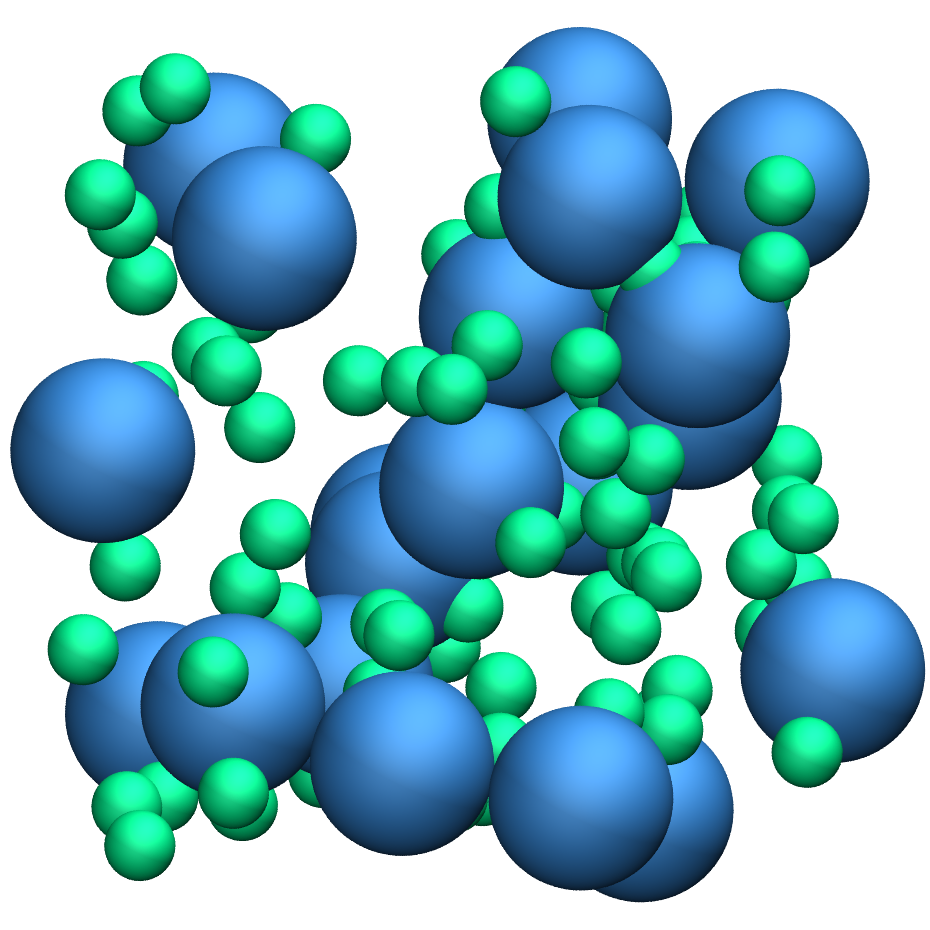
\includegraphics[width=0.55\linewidth]{LJ-avatar}
\caption{The binary mixture simulated in \hyperref[lennard-jones-label]{Tutorial 1},
with the atoms of type 1 represented as small green spheres and lge atoms of type 2
as large blue spheres.}
\label{fig:LJ-avatar}
\end{figure}

\subsubsection{My first input}

To run a simulation using LAMMPS, you need to write an input script containing
a series of commands for LAMMPS to execute.  For clarity, the
input scripts for this tutorial will be divided into five categories,
which will be filled out step by step.  To set up this tutorial, select
\guicmd{Start LAMMPS Tutorial 1} from the \guicmd{Tutorials} menu of \lammpsgui{}, and
follow the instructions.  This will select (or create, if needed) a folder,
place the initial input file \flecmd{initial.lmp} in it, and
open the file in the \lammpsgui{} editor.  The editor should display the
following content:
\begin{lstlisting}
# PART A - ENERGY MINIMIZATION
# 1) Initialization
# 2) System definition
# 3) Settings
# 4) Visualization
# 5) Run
\end{lstlisting}
Everything that appears after a hash symbol ($\#$) is a comment
and ignored by LAMMPS.  \lammpsgui{} will color such comments in red.
These five categories are not required in every input script and do not
necessarily need to be in that exact order.  For instance, the \lmpcmd{Settings}
and the \lmpcmd{Visualization} categories could be inverted, or
the \lmpcmd{Visualization} category could be omitted.  However, note that
LAMMPS reads input files from top to bottom and processes each command
\emph{immediately}.  Therefore, the \lmpcmd{Initialization} and
\lmpcmd{System definition} categories must appear at the top of the
input, and the \lmpcmd{Run} category must appear at the bottom.  Also, the
specifics of some commands can change after global settings are modified, so the
order of commands in the input script is important.

\paragraph{Initialization}

In the first section of the script, called \lmpcmd{Initialization},
global parameters for the simulation are defined, such as units, boundary conditions
(e.g.,~periodic or non-periodic), and atom types (e.g.,~uncharged point particles
or extended spheres with a radius and angular velocities).  These commands must be
executed \emph{before} creating the simulation box or they will cause
an error.  Similarly, many LAMMPS commands may only be
entered \emph{after} the simulation box is defined.  Only a limited
number of commands may be used in both cases.  Update the \flecmd{initial.lmp} file
so that the \lmpcmd{Initialization} section appears as follows:
\begin{lstlisting}
# 1) Initialization
units lj
dimension 3
atom_style atomic
boundary p p p
\end{lstlisting}
The first line, \lmpcmd{units lj}, specifies the use of
\emph{reduced} units, where all quantities are dimensionless.  This unit system is
a popular choice for simulations that explore general statistical mechanical
principles, as it emphasizes relative differences between parameters rather than
representing any specific material.  The second line, \lmpcmd{dimension 3}, specifies that the simulation is conducted
in 3D space, as opposed to 2D, where atoms are confined to move only in the
xy-plane.  The third line, \lmpcmd{atom\_style atomic}, designates
the atomic style for representing simple, individual particles.
In this style, each particle is treated as a point with a mass, making it the
most basic atom style.  Other atom styles can incorporate additional attributes for atoms,
such as charges, bonds, or molecule IDs, depending on the requirements of the simulated model.
The last line, \lmpcmd{boundary p p p}, indicates that periodic boundary
conditions are applied along all three directions of space, where the three
p stand for $x$, $y$, and $z$, respectively.  Alternatives are fixed non-periodic
(f), shrink-wrapped non-periodic (s), and shrink-wrapped non-periodic
with minimum (m).  For non-periodic boundaries, different options
can be assigned to each dimension, making configurations like \lmpcmd{boundary p p fm}
valid for systems such as slab geometries.

\begin{note}
Strictly speaking, none of the four commands specified in the
Initialization section are mandatory, as
they correspond to the default settings for their respective global properties.
However, explicitly specifying these defaults is considered good practice
to avoid confusion when sharing input files with other LAMMPS users.
\end{note}

\begin{figure}
\centering
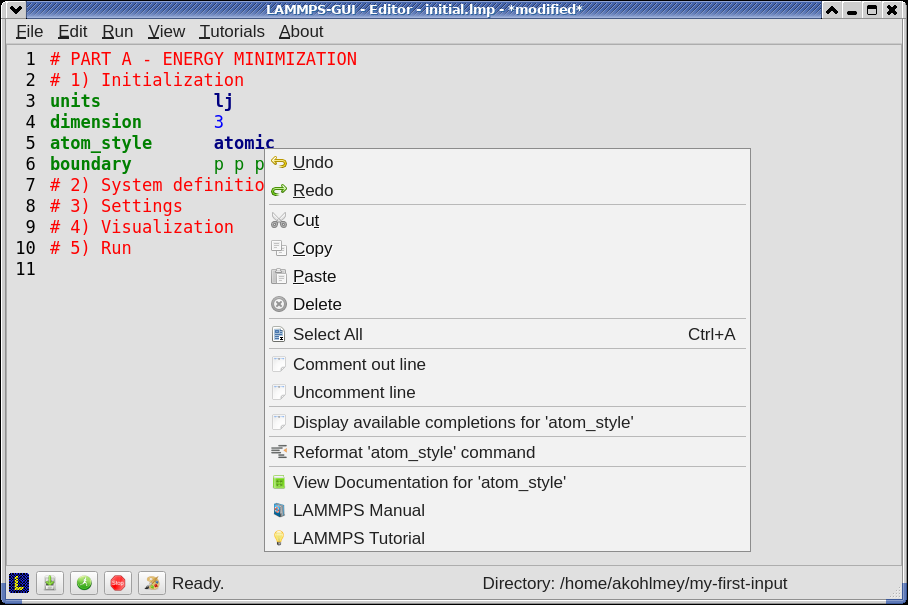
\includegraphics[width=\linewidth]{GUI-1.png}
\caption{A screenshot of the \lammpsgui{} \guicmd{Editor} window during
  \hyperref[lennard-jones-label]{Tutorial 1}.  The coloring of the text
  is based on the syntax for LAMMPS input files.  The pop-up menu is the
  context menu for right-clicking on the \lmpcmd{units lj} command.}
\label{fig:GUI-1}
\end{figure}

Each LAMMPS command is accompanied by extensive online documentation
that details the different options for that command.  From the \lammpsgui{}
editor buffer, you can access the documentation by
right-clicking on a line containing a command (e.g.,~\lmpcmd{units lj}) and
selecting \guicmd{View Documentation for `units'}.  This action will
prompt your web browser to open the corresponding URL for the online manual.
A screenshot of this context menu is shown in Fig.~\ref{fig:GUI-1}.

\paragraph{System definition}

The next step is to create the simulation box and populate it with atoms.
Modify the \lmpcmd{System definition} category of \flecmd{initial.lmp} as shown below:
\begin{lstlisting}
# 2) System definition
region simbox block -20 20 -20 20 -20 20
create_box 2 simbox
create_atoms 1 random 1500 34134 simbox overlap 0.3
create_atoms 2 random 100 12756 simbox overlap 0.3
\end{lstlisting}
The first line, \lmpcmd{region simbox (...)}, defines a region
named \lmpcmd{simbox} that is a block (i.e.,~a rectangular
cuboid) extending from -20 to 20 units along all three spatial dimensions.
The second line, \lmpcmd{create\_box 2 simbox}, initializes a simulation box
based on the region \lmpcmd{simbox} and reserves space for two types of atoms.

\begin{note}
From this point on, any command referencing an atom type larger than 2
will trigger an error.  While it is possible to allocate more atom types
than needed, you must assign a mass and provide force field parameters for
each type.  Failing to do so will cause LAMMPS to terminate with an error.
\end{note}

The third line, \lmpcmd{create\_atoms (\dots)}, generates 1500 atoms of type
1 at random positions within the
\lmpcmd{simbox} region.  The integer 34134 is a seed for the
internal random number generator, which can be changed to produce different
sequences of random numbers and, consequently, different initial atom positions.
The fourth line adds 100 atoms of type 2.
Both \lmpcmd{create\_atoms} commands use the optional argument
\lmpcmd{overlap 0.3}, which enforces a minimum distance of 0.3
units between the randomly placed atoms.  This constraint helps avoid
``close contacts'' between atoms, which can lead to excessively
large forces and simulation instability.

\paragraph{Settings}

Next, we specify the settings for the two atom types.  Modify the
\lmpcmd{Settings} category of \flecmd{initial.lmp} as follows:
\begin{lstlisting}
# 3) Settings
mass 1 1.0
mass 2 5.0
pair_style lj/cut 4.0
pair_coeff 1 1 1.0 1.0
pair_coeff 2 2 0.5 3.0
\end{lstlisting}
The two \lmpcmd{mass} commands assign a mass of 1.0 and 5.0 units
to the atoms of type 1 and 2, respectively.  The third line,
\lmpcmd{pair\_style lj/cut 4.0}, specifies that the atoms
will be interacting through a Lennard-Jones (LJ) potential with a
cut-off equal to $r_c = 4.0$ length units \cite{wang2020lennard,fischer2023history}:
\begin{equation}
E_{ij} (r) = 4 \epsilon_{ij} \left[ \left( \dfrac{\sigma_{ij}}{r} \right)^{12}
  - \left( \dfrac{\sigma_{ij}}{r} \right)^{6} \right], ~ \text{for} ~ r < r_c,
\label{eq:LJ}
\end{equation}
where $r$ is the inter-particle distance, $\epsilon_{ij}$ is
the depth of the potential well that determines the interaction strength, and
$\sigma_{ij}$ is the distance at which the potential energy equals zero.
The indexes $i$ and $j$ refer to pairs of particle types.
The fourth line, \lmpcmd{pair\_coeff 1 1 1.0 1.0}, specifies the
Lennard-Jones coefficients for interactions between pairs of atoms
of type 1: the energy parameter $\epsilon_{11} = 1.0$ and
the distance parameter $\sigma_{11} = 1.0$.  Similarly, the last line
sets the Lennard-Jones coefficients for interactions between atoms
of type 2, $\epsilon_{22} = 0.5$, and $\sigma_{22} = 3.0$.

\begin{note}
By default, LAMMPS calculates the cross coefficients for different atom
types using geometric average: $\epsilon_{ij} = \sqrt{\epsilon_{ii} \epsilon_{jj}}$,
$\sigma_{ij} = \sqrt{\sigma_{ii} \sigma_{jj}}$.  In the present case,
$\epsilon_{12} = \sqrt{1.0 \times 0.5} = 0.707$, and
$\sigma_{12} = \sqrt{1.0 \times 3.0} = 1.732$.
\end{note}

\paragraph{Single-point energy}

\begin{figure}
\centering
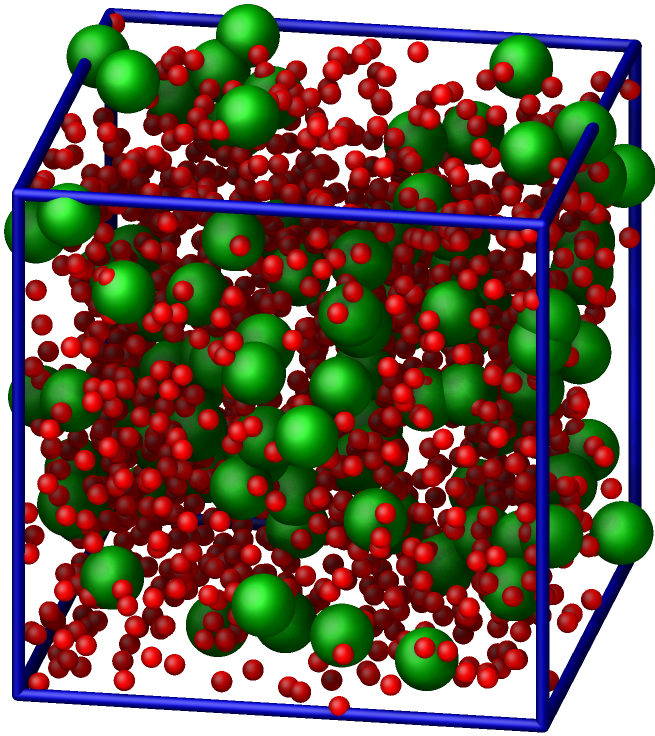
\includegraphics[width=0.55\linewidth]{LJ}
\caption{The binary mixture simulated in \hyperref[lennard-jones-label]{Tutorial 1}.
  This image was generated directly from the \lammpsgui{}.  Atoms of
  type 1 are represented as small red spheres, atoms of type 2 as large
  green spheres, and the edges of the simulation box are represented as blue sticks.}
\label{fig:LJ}
\end{figure}

The system is now fully parameterized, and the input is ready to compute
forces.  Let us complete the two remaining categories,
\lmpcmd{Visualization} and \lmpcmd{Run}, by adding the following lines
to \flecmd{initial.lmp}:
\begin{lstlisting}
# 4) Visualization
thermo 10
thermo_style custom step etotal press
# 5) Run
run 0 post no
\end{lstlisting}
The \lmpcmd{thermo 10} command instructs LAMMPS to print thermodynamic
information to the console every specified number of steps, in this case,
every 10 simulation steps.  The \lmpcmd{thermo\_style custom} command
defines the specific outputs, which in this case are the step number
(\lmpcmd{step}), total energy (\lmpcmd{etotal}), and pressure (\lmpcmd{press}).
The \lmpcmd{run 0 post no} command instructs LAMMPS to initialize forces and energy
without actually running the simulation.  The \lmpcmd{post no} option disables
the post-run summary and statistics output.

You can now run LAMMPS.  The simulation should finish quickly, and with the default
settings, \lammpsgui{} will open two windows: one displaying the console
output and another with a chart.  The \guicmd{Output} window will display information from
the executed commands, including the total energy and pressure at step 0,
as specified by the thermodynamic data request.  Since no actual simulation
steps were performed, the \guicmd{Charts} window will be empty.

\paragraph{Snapshot Image}

At this point, you can create a snapshot image of the
current system using the \guicmd{Image Viewer} window, which can be
accessed by clicking the \guicmd{Create Image} button in the \guicmd{Run} menu.
The image viewer works by instructing LAMMPS to render an image of the current system using
its internal rendering library via the \lmpcmd{dump image} command.  The
resulting image is then displayed, with various buttons available to adjust
the view and rendering style.  The image shown in
Fig.~\ref{fig:LJ} was created this way.  This will always capture the current
state of the system.  Save the image for future comparisons.

\paragraph{Energy minimization}

Now, replace the \lmpcmd{run 0 post no} command line with the
following \lmpcmd{minimize} command:
\begin{lstlisting}
# 5) Run
minimize 1.0e-6 1.0e-6 1000 10000
\end{lstlisting}
This tells LAMMPS to perform an energy minimization of the system.
Specifically, LAMMPS will compute the forces on all atoms and then update their
positions according to a selected algorithm, aiming to reduce
the potential energy.  By default, LAMMPS uses the conjugate gradient (CG)
algorithm~\cite{hestenes1952methods}.  The simulation will stop as soon
as the minimizer algorithm cannot find a way to lower the potential
energy. % SG: I don't think that its true, its rather the algorithm
% will stop when one of the four criteria is met. Axel, what do you think?
% I propose to replace by "when specific convergence criteria are met"
Note that, except for trivial systems, minimization algorithms will find a
local minimum rather than the global minimum.

Run the minimization and observe that \lammpsgui{} captures the output
and update the chart in real time (see Fig.~\ref{fig:chart-log}).  This run executes quickly (depending
on your computer's capabilities), but \lammpsgui{} may fail to capture some
of the thermodynamic data.  In that
case, use the \guicmd{Preferences} dialog to reduce the data update
interval and switch to single-threaded, unaccelerated execution in the
\guicmd{Accelerators} tab.  You can repeat the run; each new attempt will start
fresh, resetting the system and re-executing the script from the beginning.

\begin{figure}
\centering
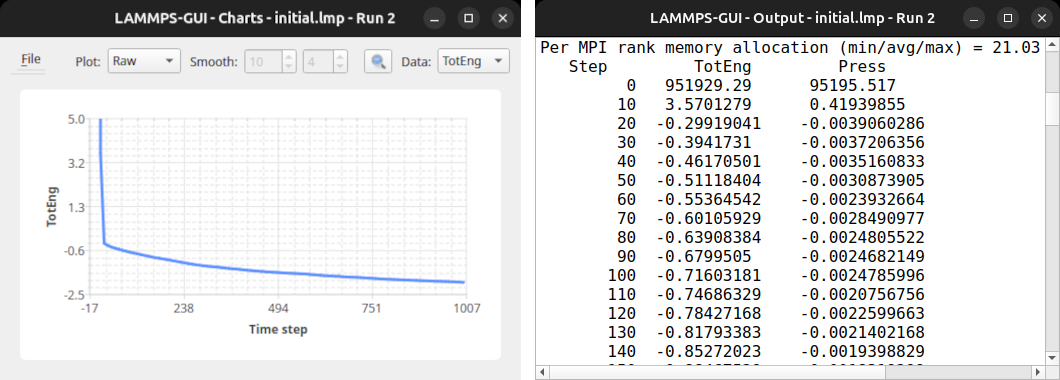
\includegraphics[width=\linewidth]{chart-and-output.png}
\caption{\guicmd{Charts} (left) and \guicmd{Output} (right) windows of \lammpsgui{}
  after performing the minimization simulation of \hyperref[lennard-jones-label]{Tutorial 1}.}
\label{fig:chart-log}
\end{figure}

The potential energy decreases from a positive value to a
negative value (Figs.~\ref{fig:chart-log} and \ref{fig:evolution-energy}\,a).
The initially positive potential energy is
expected, as the atoms are created at random positions within
the simulation box, with some in very close proximity to each other.
This proximity results in a large initial potential energy due to the repulsive branch of the
Lennard-Jones potential [i.e.,~the term in $1/r^{12}$ in Eq.~\eqref{eq:LJ}].
As the energy minimization progresses, the
energy decreases - first rapidly - then more gradually,
before plateauing at a negative value.  This indicates that the atoms
have moved to reasonable distances from one another.

Create and save a snapshot image of the simulation state after the
minimization, and compare it to the initial image.  You should observe
that the atoms are ``clumping together'' as they move toward positions
of lower potential energy.

\begin{note}
Since the \lmpcmd{thermo\_style} command also includes the \lmpcmd{press}
keyword, you can switch from plotting the total energy to
displaying the pressure by selecting \guicmd{Press} in the \guicmd{Select data}
drop-down menu of the \guicmd{Charts} window.
\end{note}

\paragraph{Molecular dynamics}

After energy minimization, any overlapping atoms are displaced, and
the system is ready for a molecular dynamics simulation.  To continue
from the result of the minimization step, append the MD simulation
commands to the same input script, \flecmd{initial.lmp}.  Add the
following lines immediately after the \lmpcmd{minimize} command:
\begin{lstlisting}
# PART B - MOLECULAR DYNAMICS
# 4) Visualization
thermo 50
thermo_style custom step temp etotal pe ke press
\end{lstlisting}

Since LAMMPS reads inputs from top to bottom, these lines will
be executed \emph{after} the energy minimization.  Therefore,
there is no need to re-initialize or re-define the
system.  The \lmpcmd{thermo} command is called a second time to
update the output frequency from 10 to 50 as soon as \lmpcmd{PART B} of
the simulation starts.  In addition, a new \lmpcmd{thermo\_style}
command is introduced to specify the thermodynamic information LAMMPS should
print during during \lmpcmd{PART B}.  This adjustment is done because during molecular
dynamics, the system exhibits non-zero temperature (\lmpcmd{temp})
and kinetic energy (\lmpcmd{ke}), which are useful to monitor.
The \lmpcmd{pe} keyword represents the potential energy of the system, such that
\lmpcmd{pe} + \lmpcmd{ke} = \lmpcmd{etotal}.

Then, add a second \lmpcmd{Run} category by including the following
lines in \lmpcmd{PART B} of \flecmd{initial.lmp}:
\begin{lstlisting}
# 5) Run
fix mynve all nve
timestep 0.005
run 50000
\end{lstlisting}
The \lmpcmd{fix nve} command updates the positions and
velocities of the atoms in the group \lmpcmd{all} at every step.  The
group \lmpcmd{all} is a default group that contains every atom.  The
last two lines specify the value of the \lmpcmd{timestep} and the number of
steps for the \lmpcmd{run}, respectively, corresponding to a total
duration of 250 time units.

\begin{note}
Since no other fix commands alter forces or velocities,
and periodic boundary conditions are applied in all directions, the MD
simulation will be performed in the microcanonical (NVE) ensemble,
which maintains a constant number of particles and a fixed box volume.
In this ensemble, the system does not exchange energy outside
the simulation box.
\end{note}

Run the simulation using LAMMPS.  Initially, there is no equilibrium
between potential and kinetic energy, as the potential energy
decreases while the kinetic energy increases.  After approximately
40\,000 steps, the values for both kinetic and potential energy
plateau, indicating that the system has reached equilibrium, with
the total energy fluctuating around a certain constant value.

Now, we change the \lmpcmd{Run} section to (note the shorter run time):
\begin{lstlisting}
# 5) Run
fix mynve all nve
fix mylgv all langevin 1.0 1.0 0.1 10917
timestep 0.005
run 15000
\end{lstlisting}
The new command adds a Langevin thermostat to the atoms in the group
\lmpcmd{all}, with a desired target temperature of 1.0 temperature units
throughout the run (the two numbers represent the target temperature at the beginning
and at the end of the run, which allows for a temperature ramp if
they differ)~\cite{schneider1978molecular}.  A \lmpcmd{damping}
parameter of 0.1 is used.  The \lmpcmd{damping} parameter determines how
rapidly the temperature is relaxed to its desired value.  In a Langevin
thermostat, the atoms are subject to friction and random noise (in the form
of randomly added velocities).  Since a constant friction term removes
more kinetic energy from fast atoms and less from slow atoms, the system
will eventually reach a dynamic equilibrium where the kinetic energy
removed and added are about the same.  The number 10917 is a
seed used to initialize the random number generator used inside of
\lmpcmd{fix langevin}; you can change it to perform statistically
independent simulations.  In the presence of a thermostat, the MD simulation
will be performed in the canonical or NVT ensemble.

Run the simulation again using LAMMPS.  From the information
printed in the \guicmd{Output} window, one can see that the temperature
starts from 0 but rapidly reaches the requested value and
stabilizes itself near $T=1$ temperature units.  One can also observe that
the potential energy, $p_\text{e}$, rapidly decreases during energy
minimization (see also Fig.~\ref{fig:evolution-energy}\,a).  After
the molecular dynamics simulation starts, $p_\text{e}$ increases until
it reaches a plateau value of about -0.25.  The kinetic energy,
$k_\text{e}$, is equal to zero during energy minimization and then
increases rapibly during molecular dynamics until it reaches
a plateau value of about 1.5 (Fig.~\ref{fig:evolution-energy}\,b).

\begin{figure}
\centering
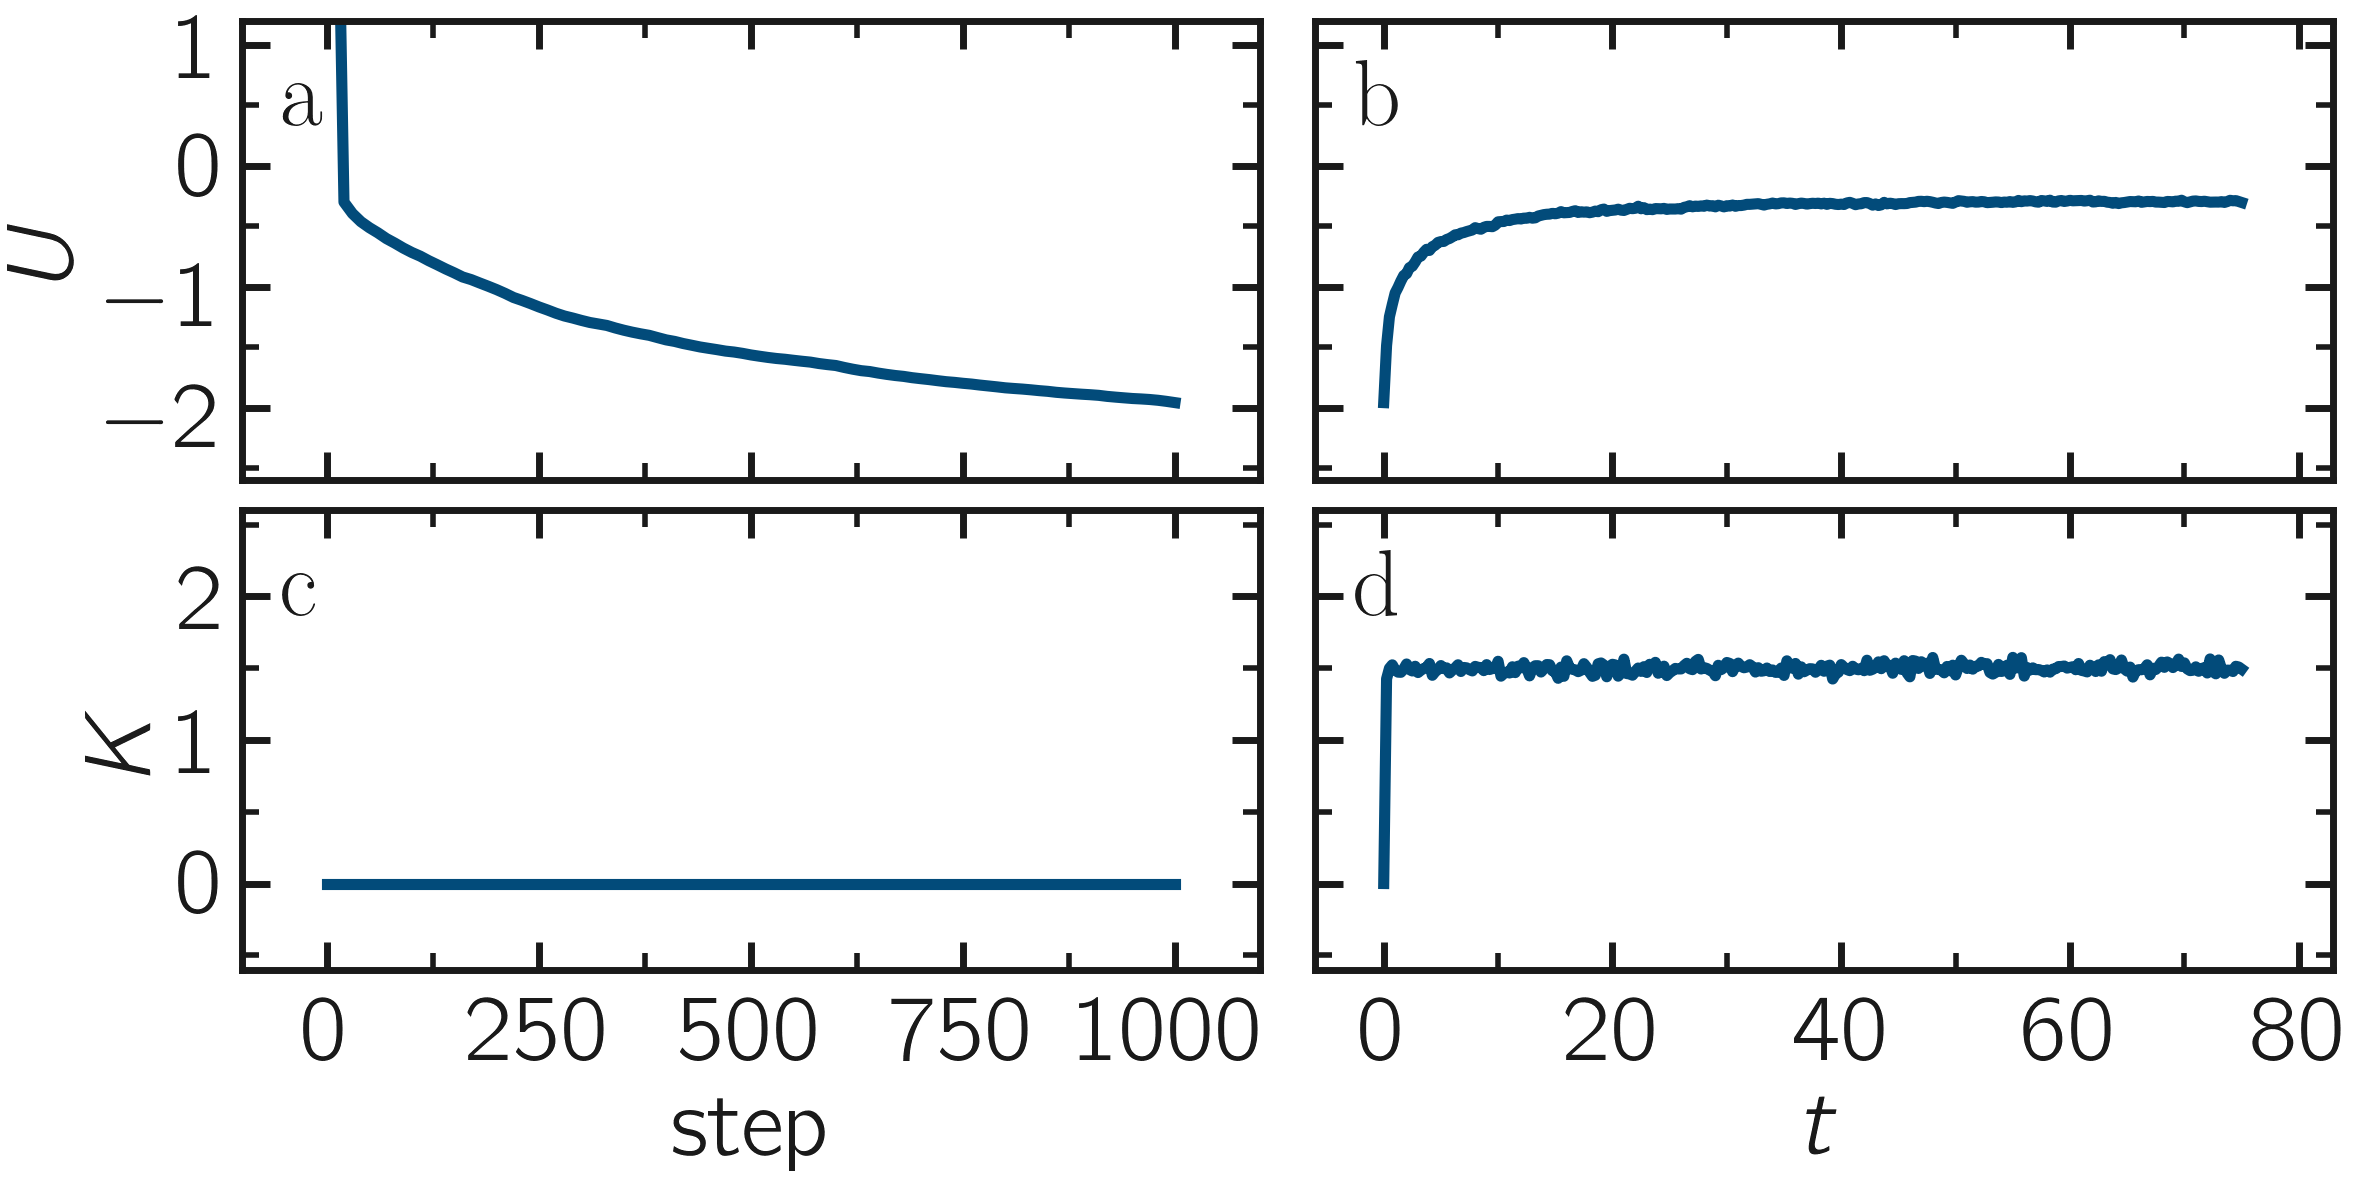
\includegraphics[width=\linewidth]{LJ-energy}
\caption{Potential energy ($p_\text{e}$) of the binary mixture simulated
during \hyperref[lennard-jones-label]{Tutorial 1} as a function of the step
during energy minimization (a) and during molecular dynamics in the NVT ensemble (b).
b)~Kinetic energy ($k_\text{e}$) during energy minimization (c) and during
molecular dynamics (d).}
\label{fig:evolution-energy}
\end{figure}

\paragraph{Trajectory visualization}

So far, the simulation has been mostly monitored through the analysis of
thermodynamic information.  To better follow the evolution of the system and visualize
the trajectories of the atoms, let us use the \lmpcmd{dump image} command to
create snapshot images during the simulation.  We have already explored
the \guicmd{Image Viewer} window.  Open it again and adjust the
visualization to your liking using the available buttons.  Now you can
copy the commands used to create this visualization to the clipboard
by either using the \guicmd{Ctrl-D} keyboard shortcut or selecting
\guicmd{Copy dump image command} from the \guicmd{File} menu.  This text
can be pasted into the into the \lmpcmd{Visualization} section of
\lmpcmd{PART B} of the \flecmd{initial.lmp} file.  This may look like the following:
\begin{lstlisting}
dump viz all image 100 myimage-*.ppm type type &
  size 800 800 zoom 1.452 shiny 0.7 fsaa yes &
  view 80 10 box yes 0.025 axes no 0.0 0.0 &
  center s 0.483725 0.510373 0.510373
dump_modify viz pad 9 boxcolor royalblue &
  backcolor white adiam 1 1.6 adiam 2 4.8
\end{lstlisting}
This command tells LAMMPS to generate NetPBM format images every 100
steps.  The two \lmpcmd{type} keywords are for \lmpcmd{color} and
\lmpcmd{diameter}, respectively.  Run the \flecmd{initial.lmp} using
LAMMPS again, and a new window named \guicmd{Slide Show} will pop up.
It will show each image created by the \lmpcmd{dump image} as it is
created. After the simulation is finished (or stopped), the slideshow
viewer allows you to animate the trajectory by cycling through the
images.  The window also allows you to export the animation to a movie
(provided the FFMpeg program is installed) and to bulk delete those
image files.

The rendering of the system can be further adjusted using the many
options of the \lmpcmd{dump image} command.  For instance, the value for the
\lmpcmd{shiny} keyword is used to adjust the shininess of the atoms, the
\lmpcmd{box} keyword adds or removes a representation of the box, and
the \lmpcmd{view} and \lmpcmd{zoom} keywords adjust the camera (and so
on).

\subsubsection{Improving the script}

Let us improve the input script and perform more advanced operations,
such as specifying initial positions for the atoms and restarting the
simulation from a previously saved configuration.

\paragraph{Control the initial atom positions}

Open the \flecmd{improved.min.lmp}, which was downloaded during the
tutorial setup.  This file contains the \lmpcmd{Part A} of the
\flecmd{initial.lmp} file, but \emph{without} any
commands in the \lmpcmd{System definition} section:
\begin{lstlisting}
# 1) Initialization
units lj
dimension 3
atom_style atomic
boundary p p p
# 2) System definition
# 3) Settings
mass 1 1.0
mass 2 10.0
pair_style lj/cut 4.0
pair_coeff 1 1 1.0 1.0
pair_coeff 2 2 0.5 3.0
# 4) Visualization
thermo 10
thermo_style custom step etotal press
# 5) Run
minimize 1.0e-6 1.0e-6 1000 10000
\end{lstlisting}

We want to create the atoms of types 1 and 2 in two separate
regions.  To achieve this, we need to add two \lmpcmd{region} commands and then
reintroduce the \lmpcmd{create\_atoms} commands, this time using the new
regions instead of the simulation box region to place the atoms:
\begin{lstlisting}
# 2) System definition
region simbox block -20 20 -20 20 -20 20
create_box 2 simbox
# for creating atoms
region cyl_in cylinder z 0 0 10 INF INF side in
region cyl_out cylinder z 0 0 10 INF INF side out
create_atoms 1 random 1000 34134 cyl_out
create_atoms 2 random 150 12756 cyl_in
\end{lstlisting}
The \lmpcmd{side in} and \lmpcmd{side out} keywords are used to define
regions representing the inside and outside of the cylinder of radius
10 length units.  Then, append a sixth section titled \lmpcmd{Save system} at the end
of the file, ensuring that the \lmpcmd{write\_data} command is placed \emph{after}
the \lmpcmd{minimize} command:
\begin{lstlisting}
# 6) Save system
write_data improved.min.data
\end{lstlisting}

\begin{note}
A key improvement to the input is the addition of the
\lmpcmd{write\_data} command.  This command writes the state
of the system to a text file called \flecmd{improved.min.data}.
This \flecmd{.data} file will be used later
to restart the simulation from the final state of the energy
minimization step, eliminating the need to repeat the system creation and minimization.
\end{note}

Run the \flecmd{improved.min.lmp} file using LAMMPS.  At the end of the simulation,
a file called \flecmd{improved.min.data} is created.  You can view the contents
of this file from the \lammpsgui{}, by right-clicking on the file name in
the editor and selecting the entry \guicmd{View file `improved.min.data'}.

The created \flecmd{.data} file contains all the information necessary to
restart the simulation, such as the number of atoms, the box size, the
masses, and the pair coefficients.  This \flecmd{.data} file also contains the final
positions of the atoms within the \lmpcmd{Atoms} section.  The first five
columns of the \lmpcmd{Atoms} section correspond (from left to right) to
the atom indexes (from 1 to the total number of atoms, 1150), the atom
types (1 or 2 here), and the positions of the atoms $x$, $y$, $z$.  The
last three columns are image flags that keep track of which atoms
crossed the periodic boundary.  The exact format of each line in the
\lmpcmd{Atoms} section depends on the choice of \lmpcmd{atom\_style}, which
determines which per-atom data is set and stored internally in LAMMPS.

\begin{note}
Instead of the \lmpcmdnote{write\_data} command, you can also use the
\lmpcmdnote{write\_restart} command to save the state
of the simulation to a binary restart file.  Binary restart files are
more compact, faster to write, and contain more information, making them often
more convenient to use.  For example, the choice of \lmpcmdnote{atom\_style}
or \lmpcmdnote{pair\_style} is recorded, so those commands do not need to be issued
before reading the restart.  Note however that restart files are not expected to be
portable across LAMMPS versions or platforms.  Therefore, in these tutorials,
and with the exception of \hyperref[all-atom-label]{Tutorial 3}, we primarily use \lmpcmdnote{write\_data} to provide you with a reference
copy of the data file that works regardless of your LAMMPS version and platform.
\end{note}

\paragraph{Restarting from a saved configuration}

\begin{figure}
\centering
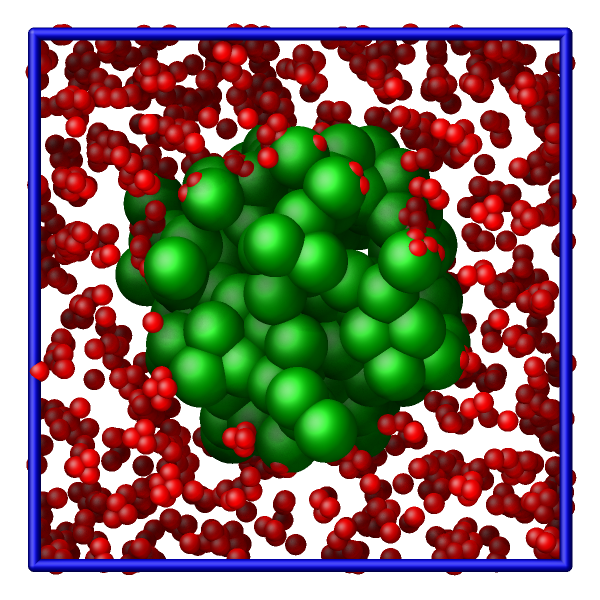
\includegraphics[width=0.55\linewidth]{LJ-cylinder}
\caption{Improved visualization of the binary mixture simulated
during \hyperref[lennard-jones-label]{Tutorial 1}.  The atoms of type 1 are
represented as small red spheres, the atoms of type 2 as large green spheres,
and the edges of the simulation box are represented as blue sticks.}
\label{fig:improved-min}
\end{figure}

To continue a simulation from the saved configuration, open the
\flecmd{improved.md.lmp} file, which was downloaded during the tutorial setup.
This file contains the \textit{Initialization} part from \flecmd{initial.lmp}
and \flecmd{improved.min.lmp}:
\begin{lstlisting}
# 1) Initialization
units lj
dimension 3
atom_style atomic
boundary p p p
# 2) System definition
# 3) Settings
# 4) Visualization
# 5) Run
\end{lstlisting}
Since we read most of the information from the data file, we don't need
to repeat all the commands from the \lmpcmd{System definition}
and \lmpcmd{Settings} categories.  The exception is the \lmpcmd{pair\_style}
command, which now must come \emph{before} the simulation box is defined,
meaning before the \lmpcmd{read\_data} command.  Add the following
lines to \flecmd{improved.md.lmp}:
\begin{lstlisting}
# 2) System definition
pair_style lj/cut 4.0
read_data improved.min.data
\end{lstlisting}

By visualizing the system (see Fig.~\ref{fig:improved-min}), you may
have noticed that some atoms left their original region during
minimization.  To start the simulation from a clean slate, with only
atoms of type 2 inside the cylinder and atoms of type 1 outside the
cylinder, let us delete the misplaced atoms by adding the following
commands to \flecmd{improved.md.lmp}:
\begin{lstlisting}
region cyl_in cylinder z 0 0 10 INF INF side in
region cyl_out cylinder z 0 0 10 INF INF side out
group grp_t1 type 1
group grp_t2 type 2
group grp_in region cyl_in
group grp_out region cyl_out
group grp_t1_in intersect grp_t1 grp_in
group grp_t2_out intersect grp_t2 grp_out
delete_atoms group grp_t1_in
delete_atoms group grp_t2_out
\end{lstlisting}
The first two \lmpcmd{region} commands recreate the previously defined
regions, which is necessary since regions are not saved by the
\lmpcmd{write\_data} command.  The first two \lmpcmd{group} commands
create groups containing all the atoms of type 1 and all the
atoms of type 2, respectively.  The next two \lmpcmd{group} commands
create atom groups based on their positions at the beginning of the
simulation, i.e.,~when the commands are being read by LAMMPS.  The last
two \lmpcmd{group} commands create atom groups based on the intersection
between the previously defined groups.  Finally, the two
\lmpcmd{delete\_atoms} commands delete the atoms of type 1
located inside the cylinder and the atoms of type 2 located
outside the cylinder, respectively.

Since LAMMPS has a limited number of custom groups (30), it is good practice
to delete groups that are no longer needed.  This can be done by adding the
following four commands to \flecmd{improved.md.lmp}:
\begin{lstlisting}
# delete unnecessary groups
group grp_in delete
group grp_out delete
group grp_t1_in delete
group grp_t2_out delete
\end{lstlisting}

Let us monitor the number of atoms of each type inside the cylinder as a
function of time by creating the following equal-style variables:
\begin{lstlisting}
variable n1_in equal count(grp_t1,cyl_in)
variable n2_in equal count(grp_t2,cyl_in)
\end{lstlisting}
The equal-style \lmpcmd{variables} are expressions evaluated
during the run and return a number.  Here, they are defined to count
the number of atoms of a specific group within the \lmpcmd{cyl\_in} region.

In addition to counting the atoms in each region, we will also extract
the coordination number of type 2 atoms around type 1 atoms.  The
coordination number measures the number of type 2 atoms near
type 1 atoms, defined by a cutoff distance.  Taking the average provides
as a good indicator of the degree of mixing in a binary mixture.  This
is done using two \lmpcmd{compute} commands:  the first counts the
coordinated atoms, and the second calculates the average over all type 1
atoms.  Add the following lines to \flecmd{improved.md.lmp}:
\begin{lstlisting}
compute coor12 grp_t1 coord/atom cutoff 2 group grp_t2
compute sumcoor12 grp_t1 reduce ave c_coor12
\end{lstlisting}
The \lmpcmd{compute reduce ave} command is used to average the per-atom
coordination number calculated by the \lmpcmd{coord/atom}
compute command.  Compute commands are not automatically invoked; they
require a ``consumer'' command that references the compute.  In this case, the
first compute is referenced by the second, and we reference the second
in a \lmpcmd{thermo\_style custom} command (see below).

\begin{figure}
\centering
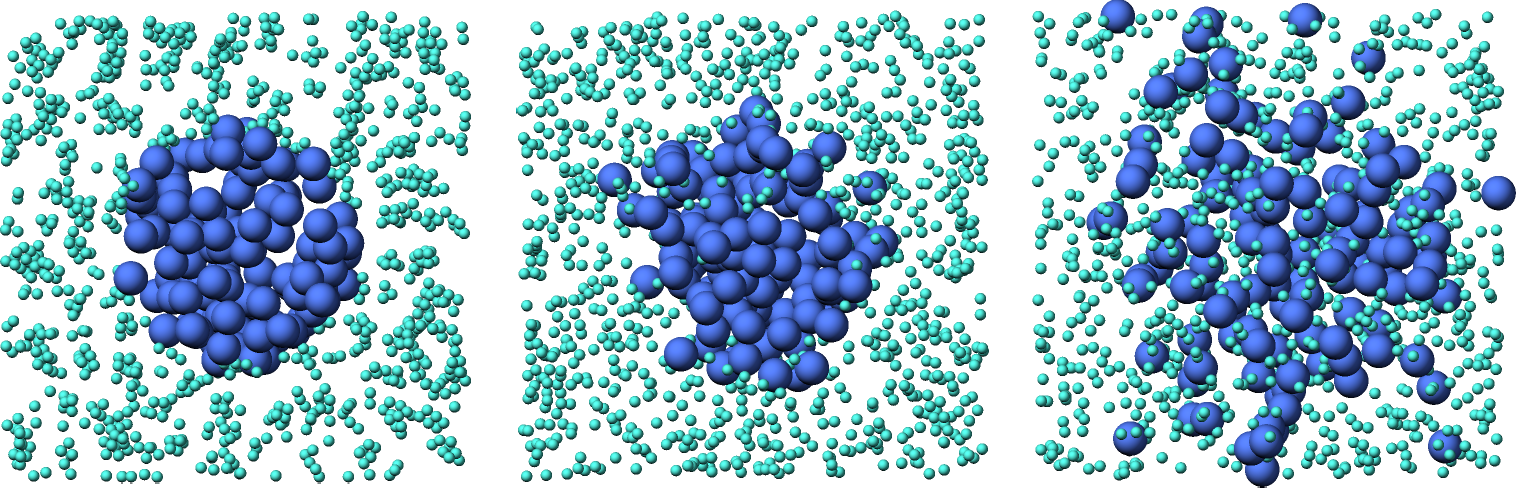
\includegraphics[width=\linewidth]{LJ-evolution}
\caption{Evolution of the system from \hyperref[lennard-jones-label]{Tutorial 1}
during mixing.  The three snapshots show respectively the system
at $t=0$ (left panel), $t=75$ (middle panel), and $t=1500$ (right panel).  The
atoms of type 1 are represented as small turquoise spheres and the atoms of type 2
as large blue spheres.}
\label{fig:evolution-population}
\end{figure}

\begin{note}
There is no need for a \lmpcmd{Settings}
section, as the settings are taken from the \flecmd{.data} file.
\end{note}

Finally, let us complete the script by adding the following lines to
\flecmd{improved.md.lmp}:
\begin{lstlisting}
# 4) Visualization
thermo 1000
thermo_style custom step temp pe ke etotal &
  press v_n1_in v_n2_in c_sumcoor12
dump viz all image 1000 myimage-*.ppm type type &
  shiny 0.1 box no 0.01 view 0 0 zoom 1.8 fsaa yes size 800 800
dump_modify viz adiam 1 1 adiam 2 3 acolor 1 &
  turquoise acolor 2 royalblue backcolor white
\end{lstlisting}
The two variables \lmpcmd{n1\_in}, \lmpcmd{n2\_in}, along with the compute
\lmpcmd{sumcoor12}, were added to the list of information printed during
the simulation.  Additionally, images of the system will be created with
slightly less saturated colors than the default ones.

Finally, add the following lines to \flecmd{improved.md.lmp}:
\begin{lstlisting}
# 5) Run
velocity all create 1.0 49284 mom yes dist gaussian
fix mynve all nve
fix mylgv all langevin 1.0 1.0 0.1 10917 zero yes
timestep 0.005
run 300000
\end{lstlisting}
Here, there are a few more differences from the previous simulation.  First,
the \lmpcmd{velocity create} command assigns an initial velocity to each
atom.  The initial velocity is chosen so that the average initial
temperature is equal to 1.0 temperature units.  The additional keywords
ensure that no linear momentum (\lmpcmd{mom yes}) is given to the
system and that the generated velocities are distributed according to
a Gaussian distribution.  Another improvement is the \lmpcmd{zero yes}
keyword in the Langevin thermostat, which ensures that the total random
force applied to the atoms is equal to zero.

\begin{figure}
\centering
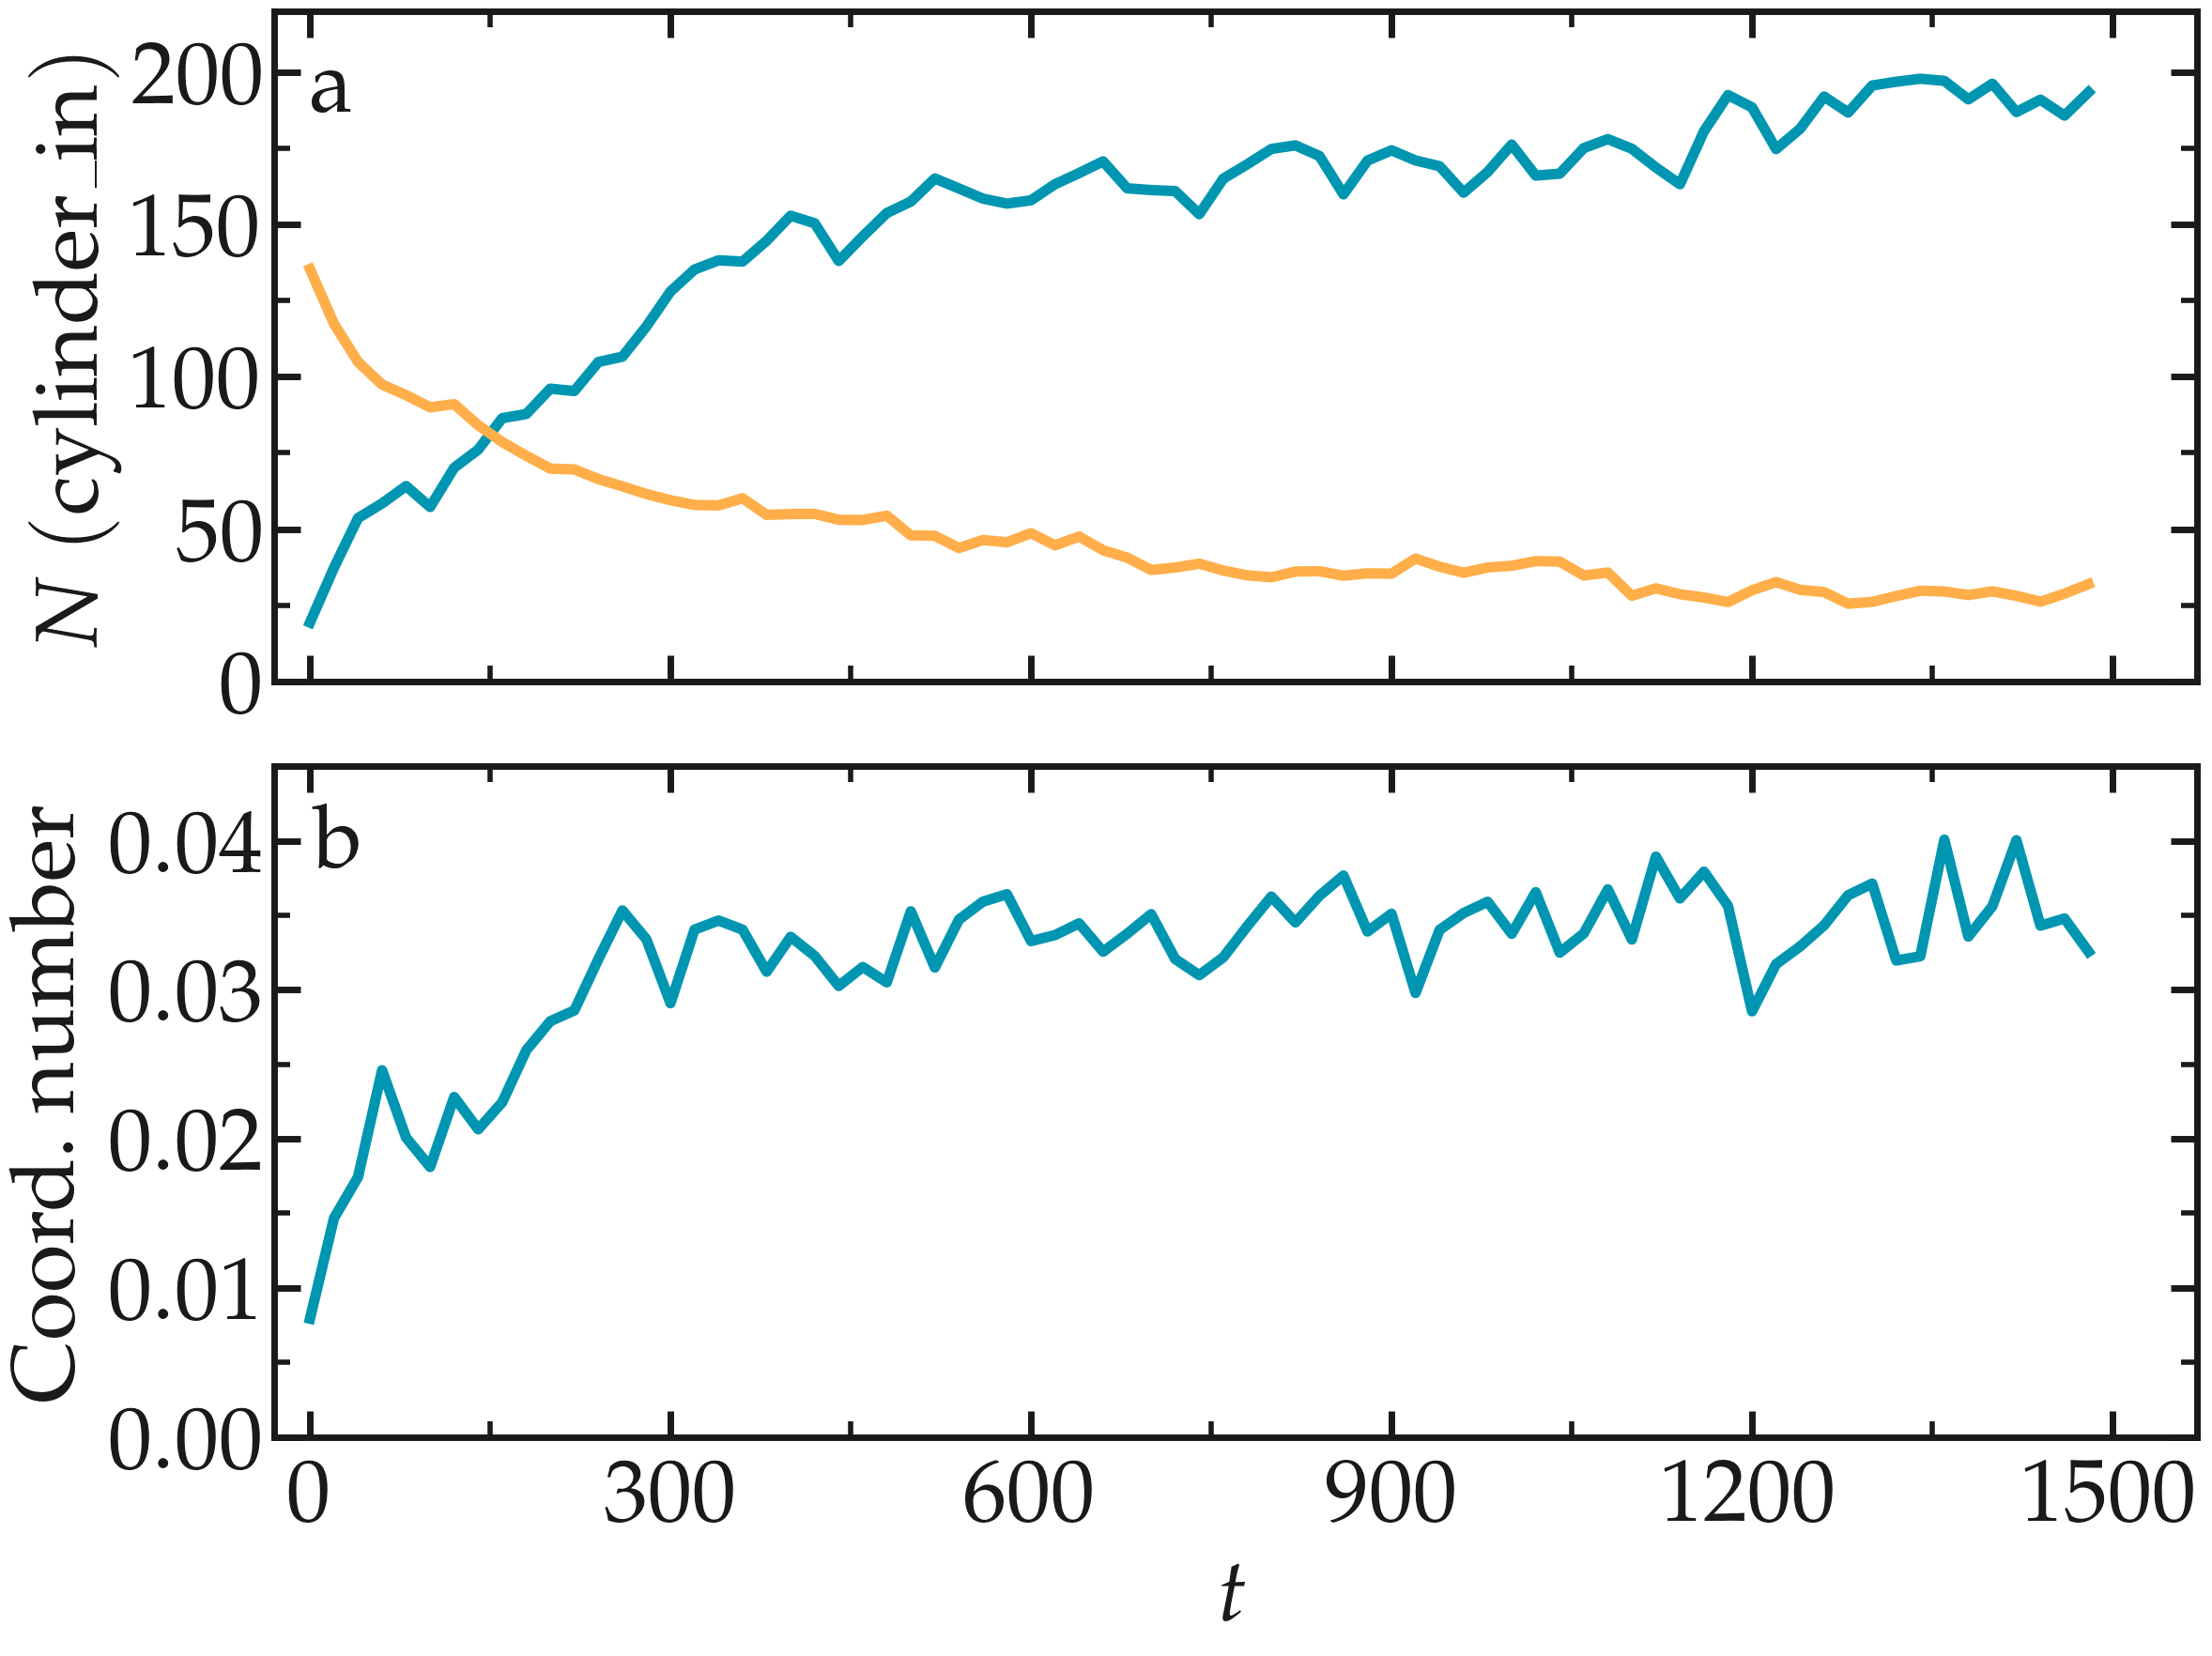
\includegraphics[width=\linewidth]{LJ-mixing}
\caption{a)~Evolution of the numbers $N_\text{1, in}$ and $N_\text{2, in}$ of atoms
of types 1 and 2, respectively, within the \lmpcmd{cyl\_in} region as functions
of time $t$.  b)~Evolution of the coordination number $C_{1-2}$ (compute \lmpcmd{sumcoor12})
between atoms of types 1 and 2.}
\label{fig:mixing}
\end{figure}

\begin{note}
The steps to ensure no initial linear momentum and no net total
force are important to prevent the system from starting to drift or move as a
whole.  For a bulk system with periodic boundary conditions, it is
expected to remain in place.  Accordingly, when computing the temperature from the
kinetic energy, we use $3N-3$ degrees of freedom since there is no
global translation.  In a drifting system, some of the kinetic energy is
due to the drift, which means the system itself cools down.  In
extreme cases, the system can freeze while its center of mass drifts very quickly.  This phenomenon is
sometimes referred to as the ``flying ice cube syndrome''~\cite{wong2016good}.
\end{note}

Run \flecmd{improved.md.lmp} and observe the mixing of the two populations
over time (see also Fig.~\ref{fig:evolution-population}).  From the
variables \lmpcmd{n1\_in} and \lmpcmd{n2\_in}, you can track the number
of atoms in each region as a function of time
(Fig.~\ref{fig:mixing}\,a).  To view their evolution, select the entries
\guicmd{v\_n1\_in} or \guicmd{v\_n2\_in} in the \guicmd{Data} drop-down
menu in the \guicmd{Charts} window of \lammpsgui{}.

In addition, as the mixing progresses, the average coordination number
between atoms of types 1 and 2 increases from about $0.01$ to $0.04$
(Fig.~\ref{fig:mixing}\,b).  This indicates that, over time, more and
more particles of type 1 come into contact with particles of type 2, as
expected during mixing.  This can be observed using the entry
\guicmd{c\_sumcoor12} in the \guicmd{Charts} drop-down menu.

\begin{figure}
\centering
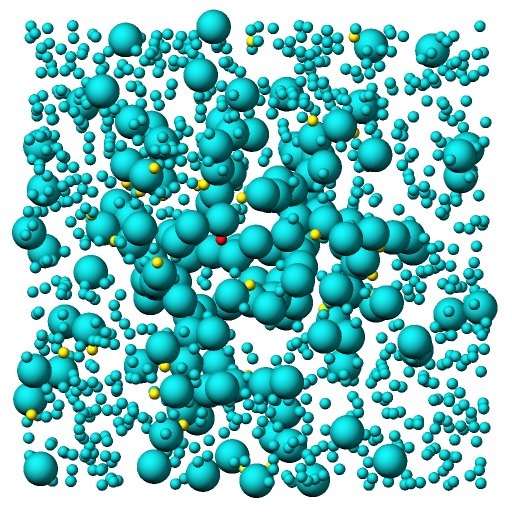
\includegraphics[width=0.55\linewidth]{LJ-coords}
\caption{Snapshot of the binary mixture simulated
  during \hyperref[lennard-jones-label]{Tutorial 1} with atoms of type 1
  colored according to their computed $1-2$ coordination
  number from the compute \lmpcmd{coor12}, ranging from turquoise,\lmpcmd{c\_coor12 = 0},
  to yellow, \lmpcmd{c\_coor12 = 1}, and red, \lmpcmd{c\_coor12 = 2}.}
\label{fig:coords-viz}
\end{figure}

\paragraph{Experiments}

Here are some suggestions for further experiments with this system that
may lead to additional insights into how different systems are configured
and how various features function:
\begin{itemize}
\item Use the Nos\'e-Hoover thermostat (\lmpcmd{fix nvt}) instead of the Langevin thermostat
  (\lmpcmd{fix nve} + \lmpcmd{fix langevin}).
\item Omit the energy minimization step before starting the MD simulation using either
the Nos\'e-Hoover or the Langevin thermostat.
\item Apply the thermostat to only one type of atoms and observe the
  temperature for each type separately.
\item Append an NVE run (i.e.~without any thermostat) and observe the energy levels.
\end{itemize}

Another useful experiment is coloring the atoms in the \guicmd{Slide Show}
according to an observable, such as their respective coordination
numbers.  To do this, replace the
\lmpcmd{dump} and \lmpcmd{dump\_modify} commands with the following lines:
\begin{lstlisting}
variable coor12 atom (type==1)*(c_coor12)+(type==2)*-1
dump viz all image 1000 myimage-*.ppm v_coor12 &
  type shiny 0.1 box no 0.01 view 0 0 zoom 1.8 fsaa yes size 800 800
dump_modify viz adiam 1 1 adiam 2 3 backcolor white &
  amap -1 2 ca 0.0 4 min royalblue 0 turquoise 1 yellow max red
\end{lstlisting}
Run LAMMPS again.  Atoms of type 1 are now colored based on the value
of \lmpcmd{c\_coor12}, which is mapped continuously from turquoise to yellow
and red for atoms with the highest coordination (Fig.~\ref{fig:coords-viz}).
In the definition of the variable \lmpcmd{v\_coor12}, atoms of type 2 are
all assigned a value of -1, and will therefore always be colored their default blue.

\subsection{Tutorial 2: Pulling on a carbon nanotube}
\label{carbon-nanotube-label}

In this tutorial, the system of interest is a small, single-walled
carbon nanotube (CNT) in an empty box (Fig.~\ref{fig:CNT}).  The CNT is
strained by imposing a constant velocity on the edge atoms.
To illustrate the difference between conventional and reactive force fields, this
tutorial is divided into two parts: in the first part, a conventional molecular force
field (called OPLS-AA~\cite{jorgensenDevelopmentTestingOPLS1996}) is
used and the bonds between the atoms of the CNT are unbreakable.  In the
second part, a reactive force field (called AIREBO
\cite{stuart2000reactive}) is used, which allows chemical bonds to break under large strain.

To set up this tutorial, select \guicmd{Start Tutorial 2} from the
\guicmd{Tutorials} menu of \lammpsgui{} and follow the instructions.  This will
select a folder, create one if necessary, and place several files into it.
The initial input file, set up for a single-point energy
calculation, will also be loaded into the editor under the name
\flecmd{unbreakable.lmp}.  Additional files are a data file containing the
CNT topology and geometry, named \flecmd{unbreakable.data}, a parameters file
named \flecmd{unbreakable.inc}, as well as the scripts required for the second part
of the tutorial.

\begin{figure}
\centering
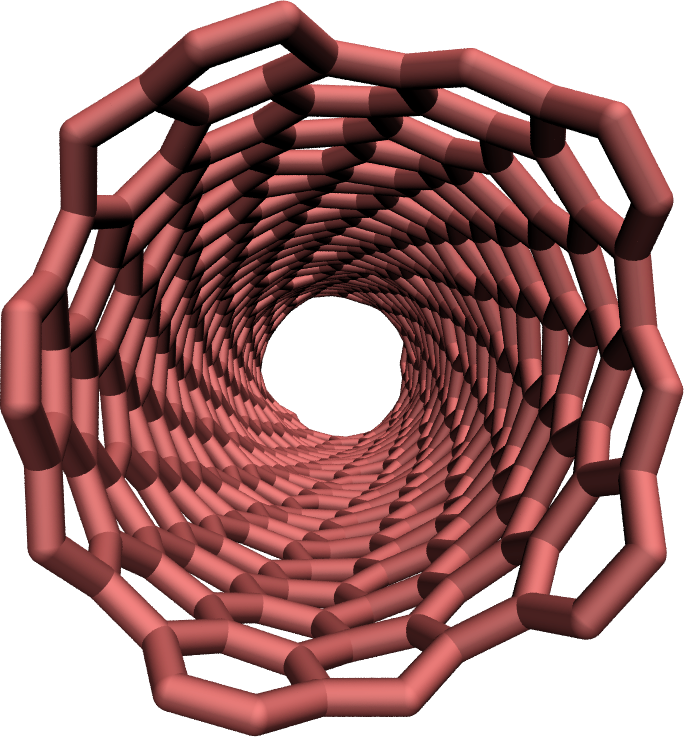
\includegraphics[width=0.55\linewidth]{CNT}
\caption{The carbon nanotube (CNT) simulated during
\hyperref[carbon-nanotube-label]{Tutorial 2}.}
\label{fig:CNT}
\end{figure}

\subsubsection{Unbreakable bonds}

With most conventional molecular force fields, the chemical bonds between
atoms are defined at the start of the simulation and remain fixed, regardless
of the forces applied to the atoms.  These bonds are typically modeled as springs
with equilibrium distances $r_0$ and force constants $k_\text{b}$:
$U_\text{b} = k_\text{b} \left( r - r_0 \right)^2$.  Additionally, angular and
dihedral constraints are often imposed to preserve the molecular structure
by maintaining the relative orientations of neighboring atoms.

\paragraph{The LAMMPS input}

After completing the setup, the editor should display the following content:
\begin{lstlisting}
units real
atom_style molecular
boundary f f f

pair_style lj/cut 14.0
bond_style harmonic
angle_style harmonic
dihedral_style opls
improper_style harmonic
special_bonds lj 0.0 0.0 0.5

read_data unbreakable.data
include unbreakable.inc

run 0 post no
\end{lstlisting}
The chosen unit system is \lmpcmd{real} (therefore distances are in
Ångstrom, times in femtosecond, and energies in kcal/mol), the
\lmpcmd{atom\_style} is \lmpcmd{molecular} (therefore atoms are point particles
that can form bonds with each other), and the boundary conditions are
fixed.  The boundary conditions do not matter here, as the box
boundaries were placed far from the CNT.  Just like in the previous
tutorial, \hyperref[lennard-jones-label]{Lennard-Jones fluid}, the pair
style is \lmpcmd{lj/cut} (i.e.~a Lennard-Jones potential with cutoff)
and its cutoff is set to 14~Ångströms, which means that only the atoms
closer than this distance interact through the Lennard-Jones potential.

The \lmpcmd{bond\_style}, \lmpcmd{angle\_style},
\lmpcmd{dihedral\_style}, and \lmpcmd{improper\_style} commands specify
the different potentials used to constrain the relative positions of the
atoms.  The \lmpcmd{special\_bonds} command sets the weighting factors
for the Lennard-Jones interactions between atoms directly connected by
one bond, two bonds, and three bonds, respectively.  This is done for
convenience when parameterizing the force constants for bonds, angles, and
so on.  By excluding the non-bonded (Lennard-Jones) interactions for
these pairs, those interactions do not need to be considered when determining
the force constants.

The \lmpcmd{read\_data} command imports the
\href{\filepath tutorial2/unbreakable.data}{\dwlcmd{unbreakable.data}}
file that should have been downloaded next
to \lmpcmd{unbreakable.lmp} during the tutorial setup. This file
contains information about the box size, atom positions, as well as the
identity of the atoms that are
linked by \lmpcmd{bonds}, \lmpcmd{angles}, \lmpcmd{dihedrals}, and
\lmpcmd{impropers} interactions. It was created using VMD and TopoTools
\cite{kohlmeyer2017topotools}.

\begin{note}
The format details of the
different sections in a data file change with different settings.  In
particular, the \lmpcmd{Atoms} section may have a different number of
columns, or the columns may represent different properties when the
\lmpcmd{atom\_style} is changed.  To help users, LAMMPS and tools like
VMD and TopoTools will add a comment (here \lmpcmd{\# molecular}) to the
\lmpcmd{Atoms} header line in the data files that indicates the intended
\lmpcmd{atom\_style}.  LAMMPS will print a warning when the chosen atom
style does not match what is written in that comment.
\end{note}

The \flecmd{.data} file does not contain any sections with potential parameters; thus,
we need to specify the parameters of both the bonded and
non-bonded potentials.  The parameters we use are taken
from the OPLS-AA (Optimized Potentials for Liquid Simulations-All-Atom)
force field~\cite{jorgensenDevelopmentTestingOPLS1996}, and are given
in a separate \lmpcmd{unbreakable.inc} file (also downloaded during
the tutorial setup).  This file - that must be placed
next to \flecmd{unbreakable.lmp} - contains the following lines:
\begin{lstlisting}
pair_coeff 1 1 0.066 3.4
bond_coeff 1 469 1.4
angle_coeff 1 63 120
dihedral_coeff 1 0 7.25 0 0
improper_coeff 1 5 180
\end{lstlisting}
% AK: the english here reads a bit "quirky". Jake, any ideas as a native speaker?
The \lmpcmd{pair\_coeff} command sets the parameters for non-bonded
Lennard-Jones interactions atom type 1 to
$\epsilon_{11} = 0.066 \, \text{kcal/mol}$ and
$\sigma_{11} = 3.4 \, \text{\AA{}}$.  The \lmpcmd{bond\_coeff} provides
the equilibrium distance $r_0= 1.4 \, \text{\AA{}}$ and the
spring constant $k_\text{b} = 469 \, \text{kcal/mol/\AA{}}^2$ for the
harmonic potential imposed between two neighboring carbon atoms.  The potential
is given by $U_\text{b} = k_\text{b} ( r - r_0)^2$.  The
\lmpcmd{angle\_coeff} gives the equilibrium angle $\theta_0$ and
constant for the potential between three neighboring atoms :
$U_\theta = k_\theta ( \theta - \theta_0)^2$.  The
\lmpcmd{dihedral\_coeff} and \lmpcmd{improper\_coeff} define the potentials
for the constraints between 4 atoms.

\begin{note}
Rather than copying the contents of the file into the input, we
incorporate it using the \lmpcmd{include} command.  Using \lmpcmd{include} allows
us to conveniently reuse the parameter settings
in other inputs or switch them with others.  This will become more general
when using type labels, which is shown in the next
tutorial~\cite{typelabel_paper}.
\end{note}

\paragraph{Prepare the initial state}

In this tutorial, a deformation will be applied to the CNT by displacing
the atoms located at its edges.  To achieve this, we will first isolate the
atoms at the two edges and place them into groups named \lmpcmd{rtop} and
\lmpcmd{rbot}.  Add the following lines to \flecmd{unbreakable.lmp},
just before the \lmpcmd{run 0} command:
\begin{lstlisting}
group carbon_atoms type 1
variable xmax equal bound(carbon_atoms,xmax)-0.5
variable xmin equal bound(carbon_atoms,xmin)+0.5
region rtop block ${xmax} INF INF INF INF INF
region rbot block INF ${xmin} INF INF INF INF
region rmid block ${xmin} ${xmax} INF INF INF INF
\end{lstlisting}
The first command includes all the atoms of type 1 (i.e.~all the atoms here)
in a group named \lmpcmd{carbon\_atoms}.
The variable $x_\text{max}$ corresponds to the coordinate of the
last atoms along $x$ minus 0.5~Ångströms, and $x_\text{min}$ to the coordinate
of the first atoms along $x$ plus 0.5~Ångströms.  Then, three regions are defined,
corresponding to the following: $x < x_\text{min}$, (\lmpcmd{rbot}, for region
bottom), $x_\text{min} > x > x_\text{max}$ (\lmpcmd{rmid}, for region middle),
and $x > x_\text{max}$ (\lmpcmd{rtop}, for region top).

Finally, let us define 3 groups of atoms corresponding to the atoms
in each of the 3 regions by adding to \flecmd{unbreakable.lmp}
just before the \lmpcmd{run 0} command:
\begin{lstlisting}
group cnt_top region rtop
group cnt_bot region rbot
group cnt_mid region rmid
set group cnt_top mol 1
set group cnt_bot mol 2
set group cnt_mid mol 3
\end{lstlisting}
With the three \lmpcmd{set} commands, we assign unique, otherwise unused
molecule IDs to atoms in those three groups.  We will use this IDs later to
assign different colors to these groups of atoms.

\begin{figure}
\centering
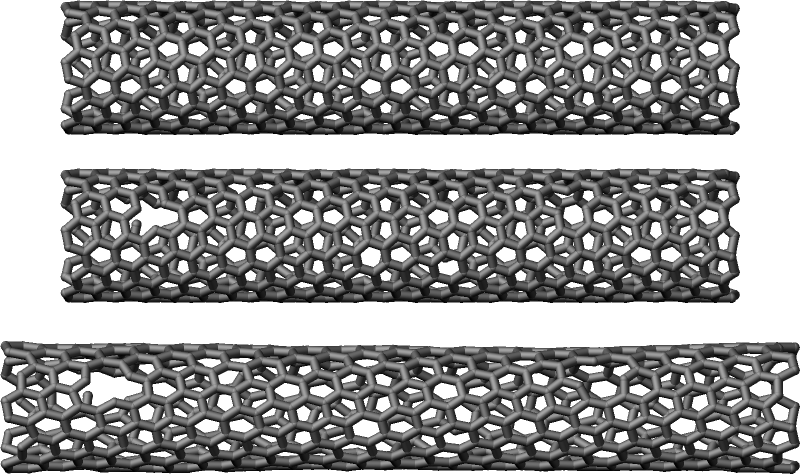
\includegraphics[width=\linewidth]{CNT-unbreakable}
\caption{The unbreakable CNT simulated during \hyperref[carbon-nanotube-label]{Tutorial 2}
before the removal of atoms (top), after the removal of 10 atoms from the \lmpcmd{rmid}
region (middle), and after deformation (bottom).}
\label{fig:CNT-unbreakable}
\end{figure}

Run the simulation using LAMMPS.  The number of atoms in each group is given in
the \guicmd{Output} window.  It is an important check to make sure that the number
of atoms in each group corresponds to what is expected, as shown here:
\begin{lstlisting}
700 atoms in group carbon_atoms
10 atoms in group cnt_top
10 atoms in group cnt_bot
680 atoms in group cnt_mid
\end{lstlisting}

Finally, to start from a less ideal state and create a system with some defects,
let us randomly delete a small fraction of the carbon atoms.  To avoid deleting
atoms that are too close to the edges, let us define a new region named \lmpcmd{rdel}
that starts at $2\,\text{\AA{}}$ from the CNT edges:
\begin{lstlisting}
variable xmax_del equal ${xmax}-2
variable xmin_del equal ${xmin}+2
region rdel block ${xmin_del} ${xmax_del} INF INF INF INF
group rdel region rdel
delete_atoms random fraction 0.02 no rdel NULL 2793 bond yes
\end{lstlisting}
The \lmpcmd{delete\_atoms} command randomly deletes $2\,\%$ of the atoms from
the \lmpcmd{rdel} group, here about 10 atoms (compare the top
and the middle panels in Fig.~\ref{fig:CNT-unbreakable}).

\paragraph{The molecular dynamics}

Let us give an initial temperature to the atoms of the group \lmpcmd{cnt\_mid}
by adding the following commands to \flecmd{unbreakable.lmp}:
\begin{lstlisting}
reset_atoms id sort yes
velocity cnt_mid create 300 48455 mom yes rot yes
\end{lstlisting}
Re-setting the atom IDs is necessary before using the \lmpcmd{velocity} command
when atoms were deleted, which is done here with the \lmpcmd{reset\_atoms} command.
The \lmpcmd{velocity} command gives initial velocities to the atoms of the middle
group \lmpcmd{cnt\_mid}, ensuring an initial temperature of $T = 300\,\text{K}$
for these atoms.

Let us specify the thermalization and the dynamics of the system.  Add the following
lines into \flecmd{unbreakable.lmp}:
\begin{lstlisting}
fix mynve1 cnt_top nve
fix mynve2 cnt_bot nve
fix mynvt cnt_mid nvt temp 300 300 100
\end{lstlisting}
The \lmpcmd{fix nve} commands are applied to the atoms of \lmpcmd{cnt\_top} and
\lmpcmd{cnt\_bot}, respectively, and will ensure that the positions of the atoms
from these groups are recalculated at every step.  The \lmpcmd{fix nvt} does the
same for the \lmpcmd{cnt\_mid} group, while also applying a Nos\'e-Hoover thermostat
with desired temperature of 300\,K~\cite{nose1984unified, hoover1985canonical}.
To restrain the motion of the atoms at the edges, let us add the following
commands to \flecmd{unbreakable.lmp}:
\begin{lstlisting}
fix mysf1 cnt_top setforce 0 0 0
fix mysf2 cnt_bot setforce 0 0 0
velocity cnt_top set 0 0 0
velocity cnt_bot set 0 0 0
\end{lstlisting}
The two \lmpcmd{setforce} commands cancel the forces applied on the atoms of the
two edges, respectively.  The cancellation of the forces is done at every step,
and along all 3 directions of space, $x$, $y$, and $z$, due to the use of
\lmpcmd{0 0 0}.  The two \lmpcmd{velocity} commands set the initial velocities
along $x$, $y$, and $z$ to 0 for the atoms of \lmpcmd{cnt\_top} and
\lmpcmd{cnt\_bot}, respectively.  As a consequence of these last four commands,
the atoms of the edges will remain immobile during the simulation (or at least
they would if no other command was applied to them).

\begin{note}
The \lmpcmdnote{velocity set}
command imposes the velocity of a group of atoms at the start of a run but does
not enforce the velocity during the entire simulation.  When \lmpcmdnote{velocity set}
is used in combination with \lmpcmdnote{setforce 0 0 0}, as is the case here, the
atoms won't feel any force during the entire simulation.  According to the Newton
equation, no force means no acceleration, meaning that the initial velocity
will persist during the entire simulation, thus producing a constant velocity motion.
\end{note}

\paragraph{Outputs}

Next, to measure the strain and stress applied to the CNT, let us create a
variable for the distance $L_\text{cnt}$ between the two edges,
as well as a variable $F_\text{cnt}$ for the force applied on the edges:
\begin{lstlisting}
variable Lcnt equal xcm(cnt_top,x)-xcm(cnt_bot,x)
variable Fcnt equal f_mysf1[1]-f_mysf2[1]
\end{lstlisting}
Here, the force is extracted from the fixes \lmpcmd{mysf1} and \lmpcmd{mysf2}
using \lmpcmd{f\_}, similarly to the use of \lmpcmd{v\_} to call a variable,
and \lmpcmd{c\_} to call a compute, as seen in \hyperref[lennard-jones-label]{Tutorial 1}.

Let us also add a \lmpcmd{dump image} command to visualize the system
every 500 steps:
\begin{lstlisting}
dump viz all image 500 myimage-*.ppm element type size &
  1000 400 zoom 6 shiny 0.3 fsaa yes bond atom 0.8 &
  view 0 90 box no 0.0 axes no 0.0 0.0
dump_modify viz pad 9 backcolor white adiam 1 0.85 bdiam 1 1.0
\end{lstlisting}
Let us run a small equilibration step to bring the system to the required
temperature before applying any deformation.  Replace the \lmpcmd{run 0 post no}
command in \flecmd{unbreakable.lmp} with the following lines:
\begin{lstlisting}
compute Tmid cnt_mid temp
thermo 100
thermo_style custom step temp etotal v_Lcnt v_Fcnt
thermo_modify temp Tmid line yaml

timestep 1.0
run 5000
\end{lstlisting}
With the \lmpcmd{thermo\_modify} command, we specify to LAMMPS that the
temperature $T_\mathrm{mid}$ of the middle group, \lmpcmd{cnt\_mid},
must be outputted, instead of the temperature of the entire system.
This choice is motivated by the presence of
frozen parts with an effective temperature of 0\,K, which makes the average
temperature of the entire system less relevant.  The \lmpcmd{thermo\_modify}
command also imposes the use of the YAML format that can easily be read by
Python (see below).

Let us impose a constant velocity deformation on the CNT
by combining the \lmpcmd{velocity set} command with previously defined
\lmpcmd{fix setforce}.  Add the following lines in the \lmpcmd{unbreakable.lmp}
file, right after the last \lmpcmd{run 5000} command:
\begin{lstlisting}
velocity cnt_top set 0.0005 0 0
velocity cnt_bot set -0.0005 0 0

run 10000
\end{lstlisting}
The chosen velocity for the deformation is $100\,\text{m/s}$, or
$0.001\,\text{\AA{}/fs}$.

\begin{figure}
\centering
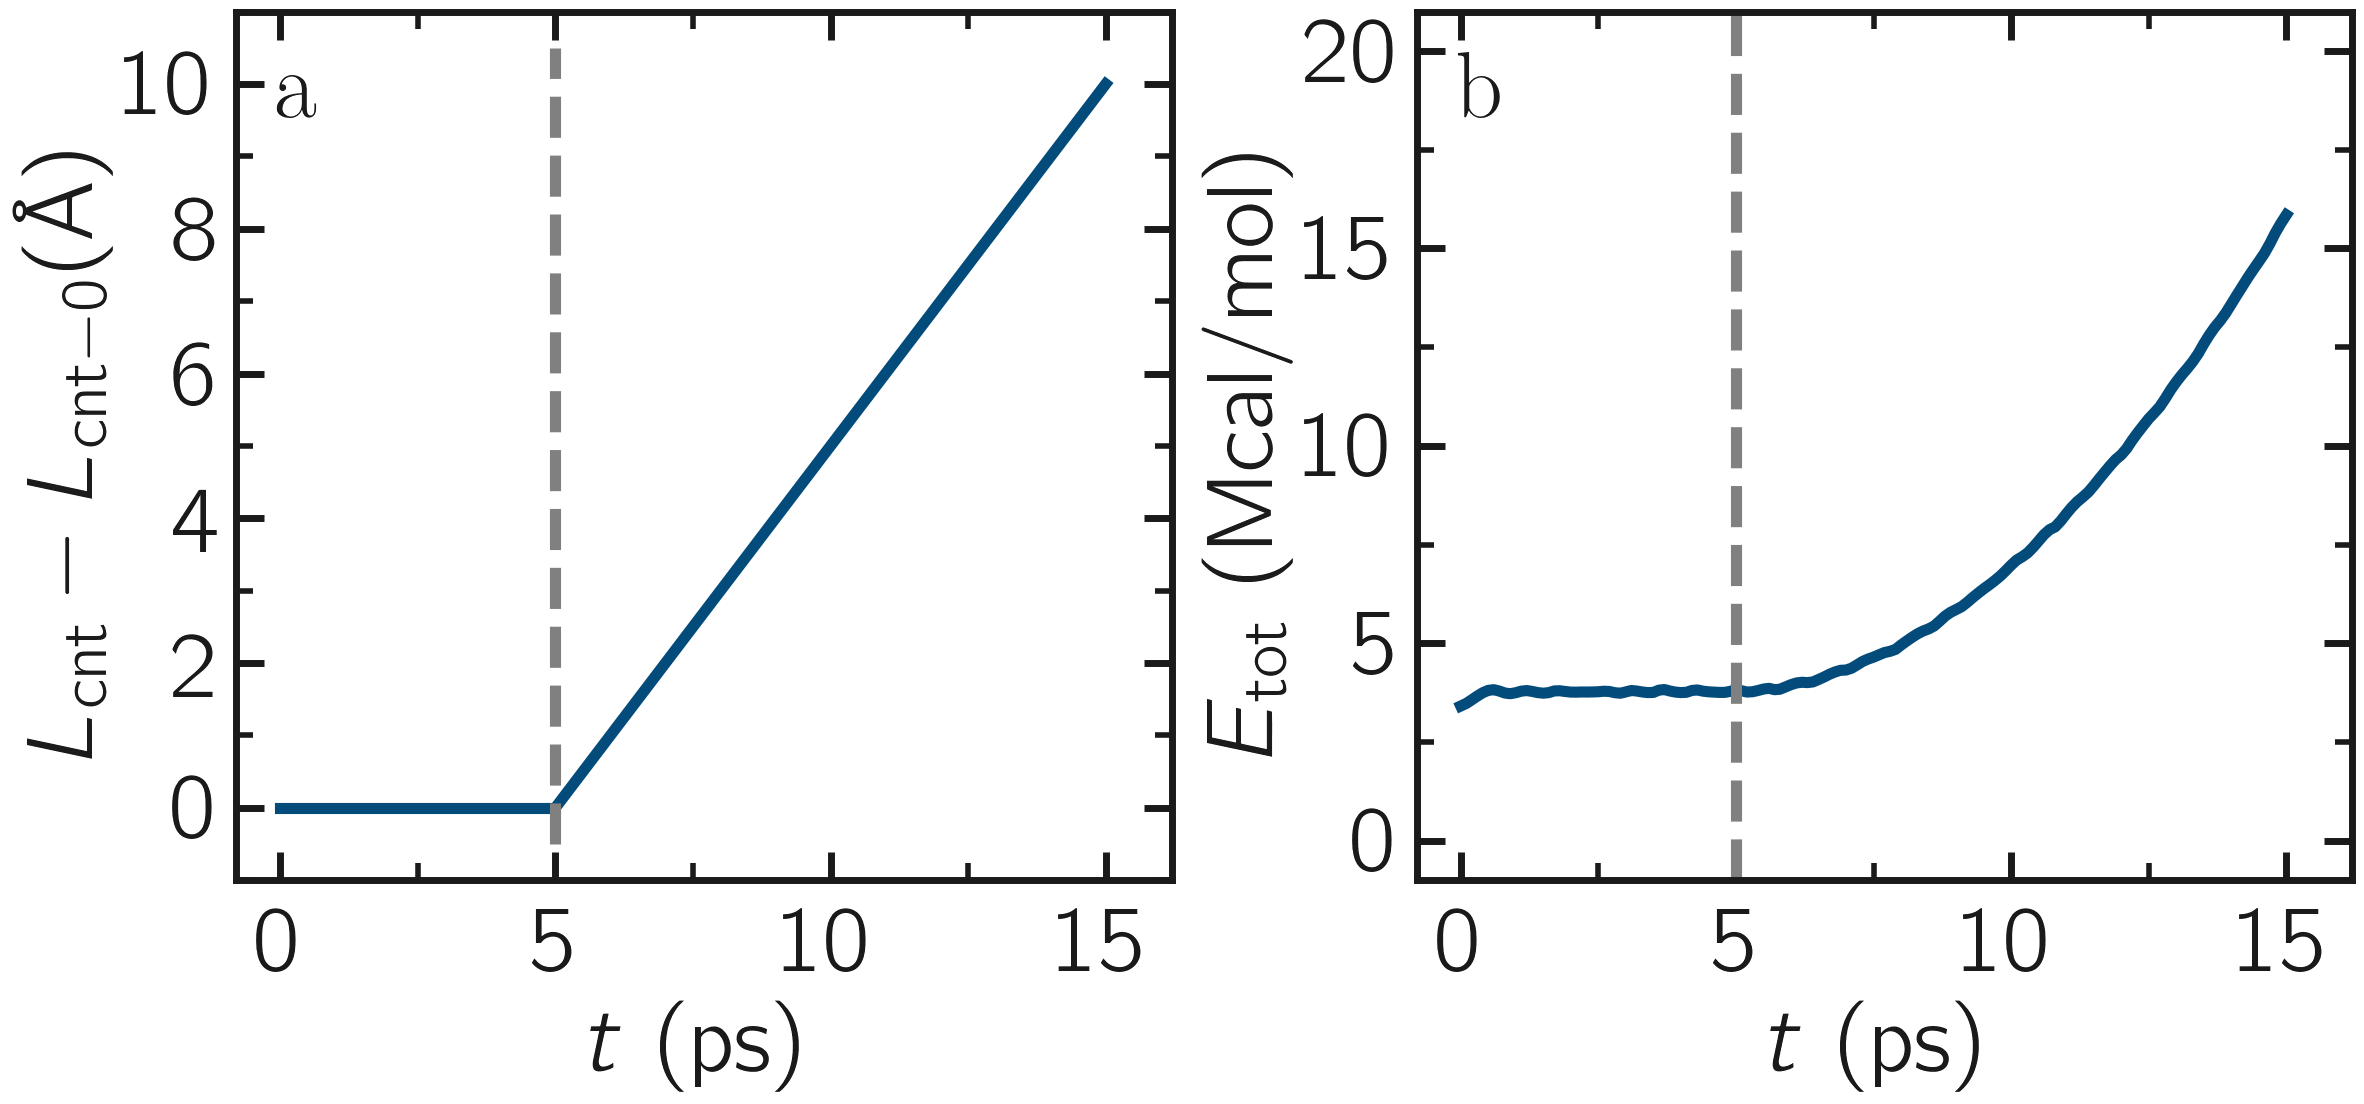
\includegraphics[width=\linewidth]{CNT-unbreakable-length-energy}
\caption{a) Evolution of the length $L_\text{cnt}$ of the CNT with time,
as simulated during \hyperref[carbon-nanotube-label]{Tutorial 2}.
The CNT starts deforming at $t = 5\,\text{ps}$, and $L_\text{cnt-0}$ is the
CNT initial length.  b) Evolution of the total energy $E_\text{tot}$ of the system
with time $t$.  Here, the potential is OPLS-AA, and the CNT is unbreakable.}
\label{fig:CNT-unbreakable-LE}
\end{figure}

Run the simulation using LAMMPS.  As can be seen from the variable $L_\text{cnt}$, the length
of the CNT increases linearly over time for $t > 5\,\text{ps}$ (Fig.~\ref{fig:CNT-unbreakable-LE}\,a),
as expected from the imposed constant velocity.  What you observe in the \guicmd{Slide Show}
windows should resembles Fig.~\ref{fig:CNT-unbreakable}.  The total energy of the system
shows a non-linear increase with $t$ once the deformation starts, which is expected
from the typical dependency of bond energy with bond distance,
$U_\text{b} = k_\text{b} \left( r - r_0 \right)^2$ (Fig.~\ref{fig:CNT-unbreakable-LE}\,b).

\paragraph{Importing YAML log file into Python}

Let us import the simulation data into Python, and generate a stress-strain curve.
Here, the stress is defined as $F_\text{cnt}/A_\text{cnt}$,
where $A_\text{cnt} = \pi r_\text{cnt}^2$ is the surface area of the
CNT, and $r_\text{cnt}=5.2$\,\AA{} the CNT radius.  The strain is defined
as $(L_\text{cnt}-L_\text{cnt-0})/L_\text{cnt-0}$, where $L_\text{cnt-0}$ is the initial CNT length.

Right-click inside the \guicmd{Output} window, and select
\guicmd{Export YAML data to file}.  Call the output \flecmd{unbreakable.yaml}, and save
it within the same folder as the input files, where a Python script named
\href{\filepath tutorial2/unbreakable-yaml-reader.py}{\dwlcmd{unbreakable-yaml-reader.py}} should also
be located.  When executed using Python, this .py file first imports
the \flecmd{unbreakable.yaml} file.  Then, a certain pattern is
identified and stored as a string character named `docs'.  The string is
then converted into a list, and $F_\text{cnt}$ and $L_\text{cnt}$
are extracted.  The stress and strain are then calculated, and the result
is saved in a data file named \flecmd{unbreakable.dat} using
the NumPy `savetxt' function.  `thermo[0]' can be used to access the
information from the first minimization run, and `thermo[1]' to access the
information from the second MD run.  The data extracted from
the \flecmd{unbreakable.yaml} file can then be used to plot the stress-strain
curve, see Fig.~\ref{fig:CNT-stress-strain-unbreakable}.

\begin{figure}
\centering
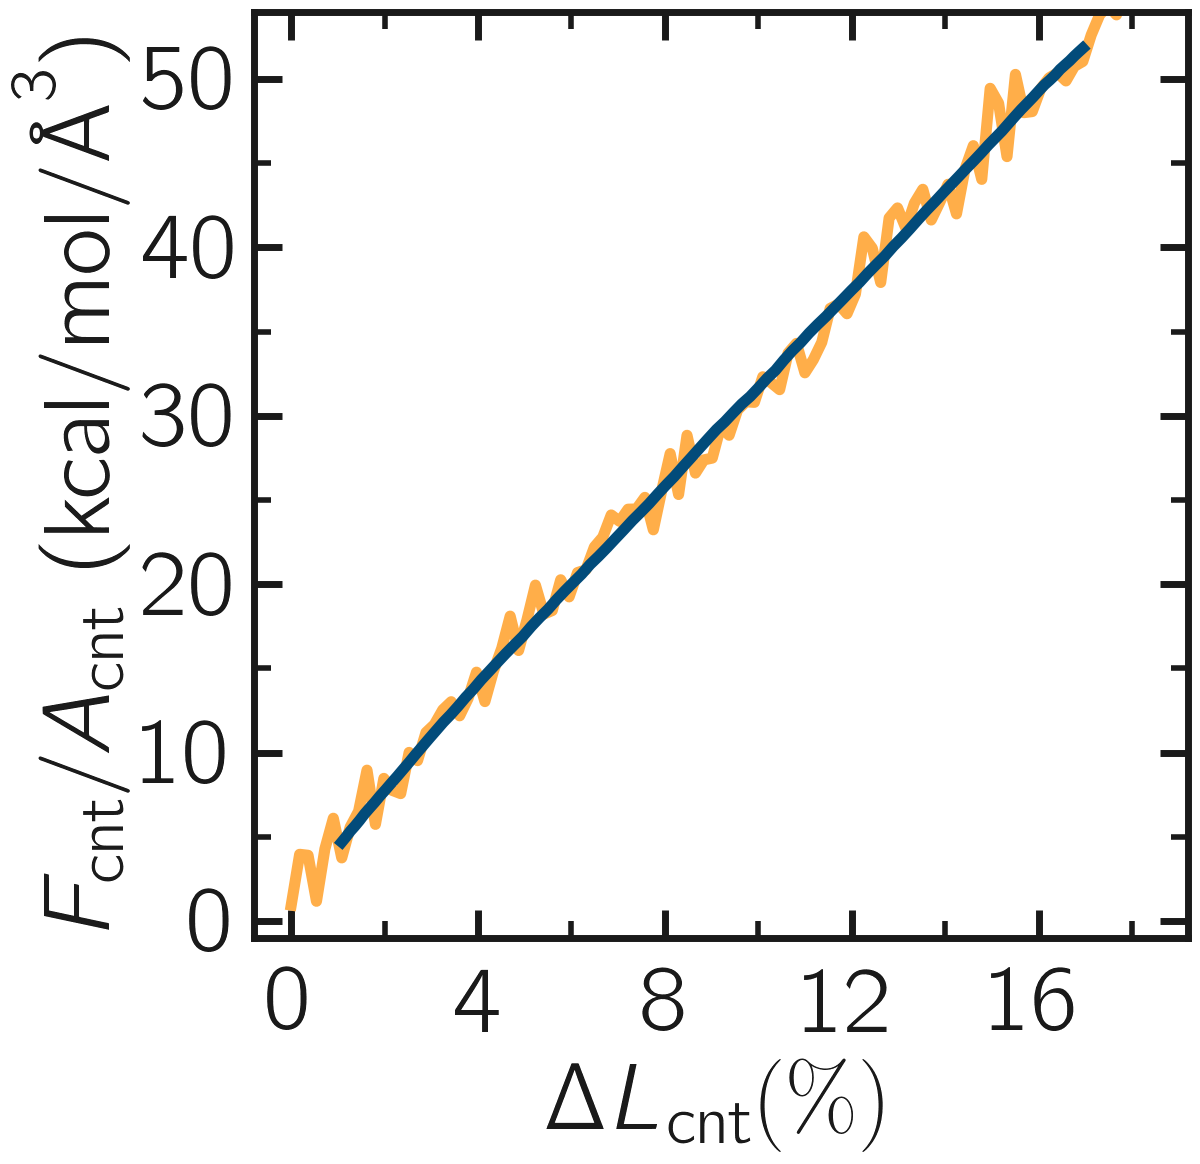
\includegraphics[width=0.55\linewidth]{CNT-unbreakable-stress-strain}
\caption{Stress applied on the CNT during deformation, $F_\text{cnt}/A_\text{cnt}$,
where $F_\text{cnt}$ is the force and $A_\text{cnt}$ the CNT surface area,
as a function of the strain, $\Delta L_\text{cnt} = (L_\text{cnt}-L_\text{cnt-0}/L_\text{cnt-0})$, where
$L_\text{cnt}$ is the CNT length and $L_\text{cnt-0}$ the CNT initial length,
as simulated during \hyperref[carbon-nanotube-label]{Tutorial 2}.
Here, the potential is OPLS-AA, and the CNT is unbreakable.}
\label{fig:CNT-stress-strain-unbreakable}
\end{figure}

\subsubsection{Breakable bonds}

When using a conventional molecular force field, as we have just done, the bonds between the atoms
are non-breakable.  Let us perform a similar simulation and deform a small
CNT again, but this time with a reactive force field that allows bonds
to break if the applied deformation is large enough.

\paragraph{Input file initialization}

Open the input named
\href{\filepath tutorial2/breakable.lmp}{\dwlcmd{breakable.lmp}} that should have
been downloaded next to \lmpcmd{unbreakable.lmp} during the tutorial setup.
There are only a few differences with the previous input.  First, the \lmpcmd{metal}
units system is used instead of \lmpcmd{real}, which is
required by the AIREBO force field.  A second difference is the use of the
\lmpcmd{atom\_style atomic} instead of \lmpcmd{molecular}, since no explicit
bond information is required with AIREBO.  The following commands are
setting up the AIREBO force field:
\begin{lstlisting}
pair_style airebo 3.0
pair_coeff * * CH.airebo C
\end{lstlisting}
Here, \href{\filepath tutorial2/CH.airebo}{\dwlcmd{CH.airebo}} is the file
containing the parameters for AIREBO, and must be placed next
to \lmpcmd{breakable.lmp}.

\begin{note}
With the \lmpcmdnote{metal} units system, times are in picoseconds ($10^{-12}$\,s)
instead of femtoseconds ($10^{-15}$\,s) in the case of the \lmpcmdnote{real} units system.
It is important to keep this in mind when setting parameters that are expressed
in time unit, such as the timestep or the time constant of the thermostat.
\end{note}

Since bonds, angles, and dihedrals do not need to be
explicitly set when using AIREBO, some simplification must be made to the
\flecmd{.data} file.  The new \flecmd{.data}
file is named \href{\filepath tutorial2/breakable.data}{\dwlcmd{breakable.data}},
and must be placed within the same folder as the input file.  Just like \flecmd{unbreakable.data},
the \flecmd{breakable.data} contains the information
required for placing the atoms in the box, but no bond/angle/dihedral information.
Another difference between the \flecmd{unbreakable.data} and \flecmd{breakable.data} files
is that, here, a larger distance of 120~Ångströms was used for the box size along
the $x$-axis, to allow for larger deformation of the CNT.

\paragraph{Start the simulation}

Here, let us perform a similar deformation as the previous one.
In \lmpcmd{breakable.lmp}, replace the \lmpcmd{run 0 post no} line with:
\begin{lstlisting}
fix mysf1 cnt_bot setforce 0 0 0
fix mysf2 cnt_top setforce 0 0 0
velocity cnt_bot set 0 0 0
velocity cnt_top set 0 0 0

variable Lcnt equal xcm(cnt_top,x)-xcm(cnt_bot,x)
variable Fcnt equal f_mysf1[1]-f_mysf2[1]

dump viz all image 500 myimage.*.ppm type type size 1000 400 &
  zoom 4 shiny 0.3 adiam 1.5 box no 0.01 view 0 90 &
  shiny 0.1 fsaa yes
dump_modify viz pad 5 backcolor white acolor 1 gray

compute Tmid cnt_mid temp
thermo 100
thermo_style custom step temp etotal v_Lcnt v_Fcnt
thermo_modify temp Tmid line yaml

timestep 0.0005
run 10000
\end{lstlisting}
Note the relatively small timestep of $0.0005$\,ps ($= 0.5$\,fs) used.  Reactive force
fields like AIREBO usually require a smaller timestep than conventional ones.  When running
\flecmd{breakable.lmp} with LAMMPS, you can see that the temperature deviates
from the target temperature of $300\,\text{K}$ at the start of the equilibration,
but that after a few steps, it reaches the target value.

\begin{note}
  Bonds cannot be displayed by the \lmpcmdnote{dump image} when using
  the \lmpcmdnote{atom\_style atomic}, as it contains no bonds.
  A tip for displaying bonds with the present system is provided at
  the end of the tutorial.
\end{note}

\paragraph{Launch the deformation}

After equilibration, let us set the velocity of the edges equal to
$75~\text{m/s}$ (or $0.75~\text{\AA{}/ps}$) and run for a longer duration than
previously.  Add the following lines into \flecmd{breakable.lmp}:
\begin{lstlisting}
velocity cnt_top set 0.75 0 0
velocity cnt_bot set -0.75 0 0

run 30000
\end{lstlisting}
Run the simulation.  Some bonds are expected to break before the end of the
simulation (Fig.~\ref{fig:CNT-deformed-breakable}).

\begin{figure}
\centering
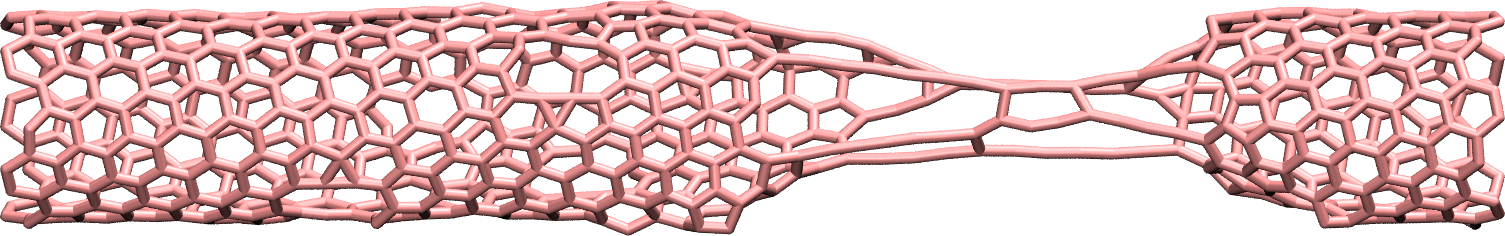
\includegraphics[width=\linewidth]{CNT-deformed-breakable}
\caption{CNT with broken bonds.  This image was generated using
VMD~\cite{vmd_home,humphrey1996vmd} with the \guicmd{DynamicBonds} representation.}
\label{fig:CNT-deformed-breakable}
\end{figure}

Looking at the evolution of the energy, one can see that the total
energy $E_\text{tot}$ is initially increasing with the deformation.  When
bonds break, the energy relaxes abruptly, as can be seen near $t=32~\text{ps}$ in Fig.~\ref{fig:CNT-breakable-energy-stress}\,a.
Using a similar script as previously,
i.e.,~\href{\filepath tutorial2/unbreakable-yaml-reader.py}{\dwlcmd{unbreakable-yaml-reader.py}},
import the data into Python and generate the stress-strain curve (Fig.~\ref{fig:CNT-breakable-energy-stress}\,b).  The
stress-strain curve reveals a linear (elastic) regime where $F_\text{cnt} \propto \Delta L_\text{cnt}$
for $\Delta L_\text{cnt} < 5\,\%$, and a non-linear (plastic) regime
for $5\,\% < \Delta L_\text{cnt} < 25\,\%$.

\begin{figure}
\centering
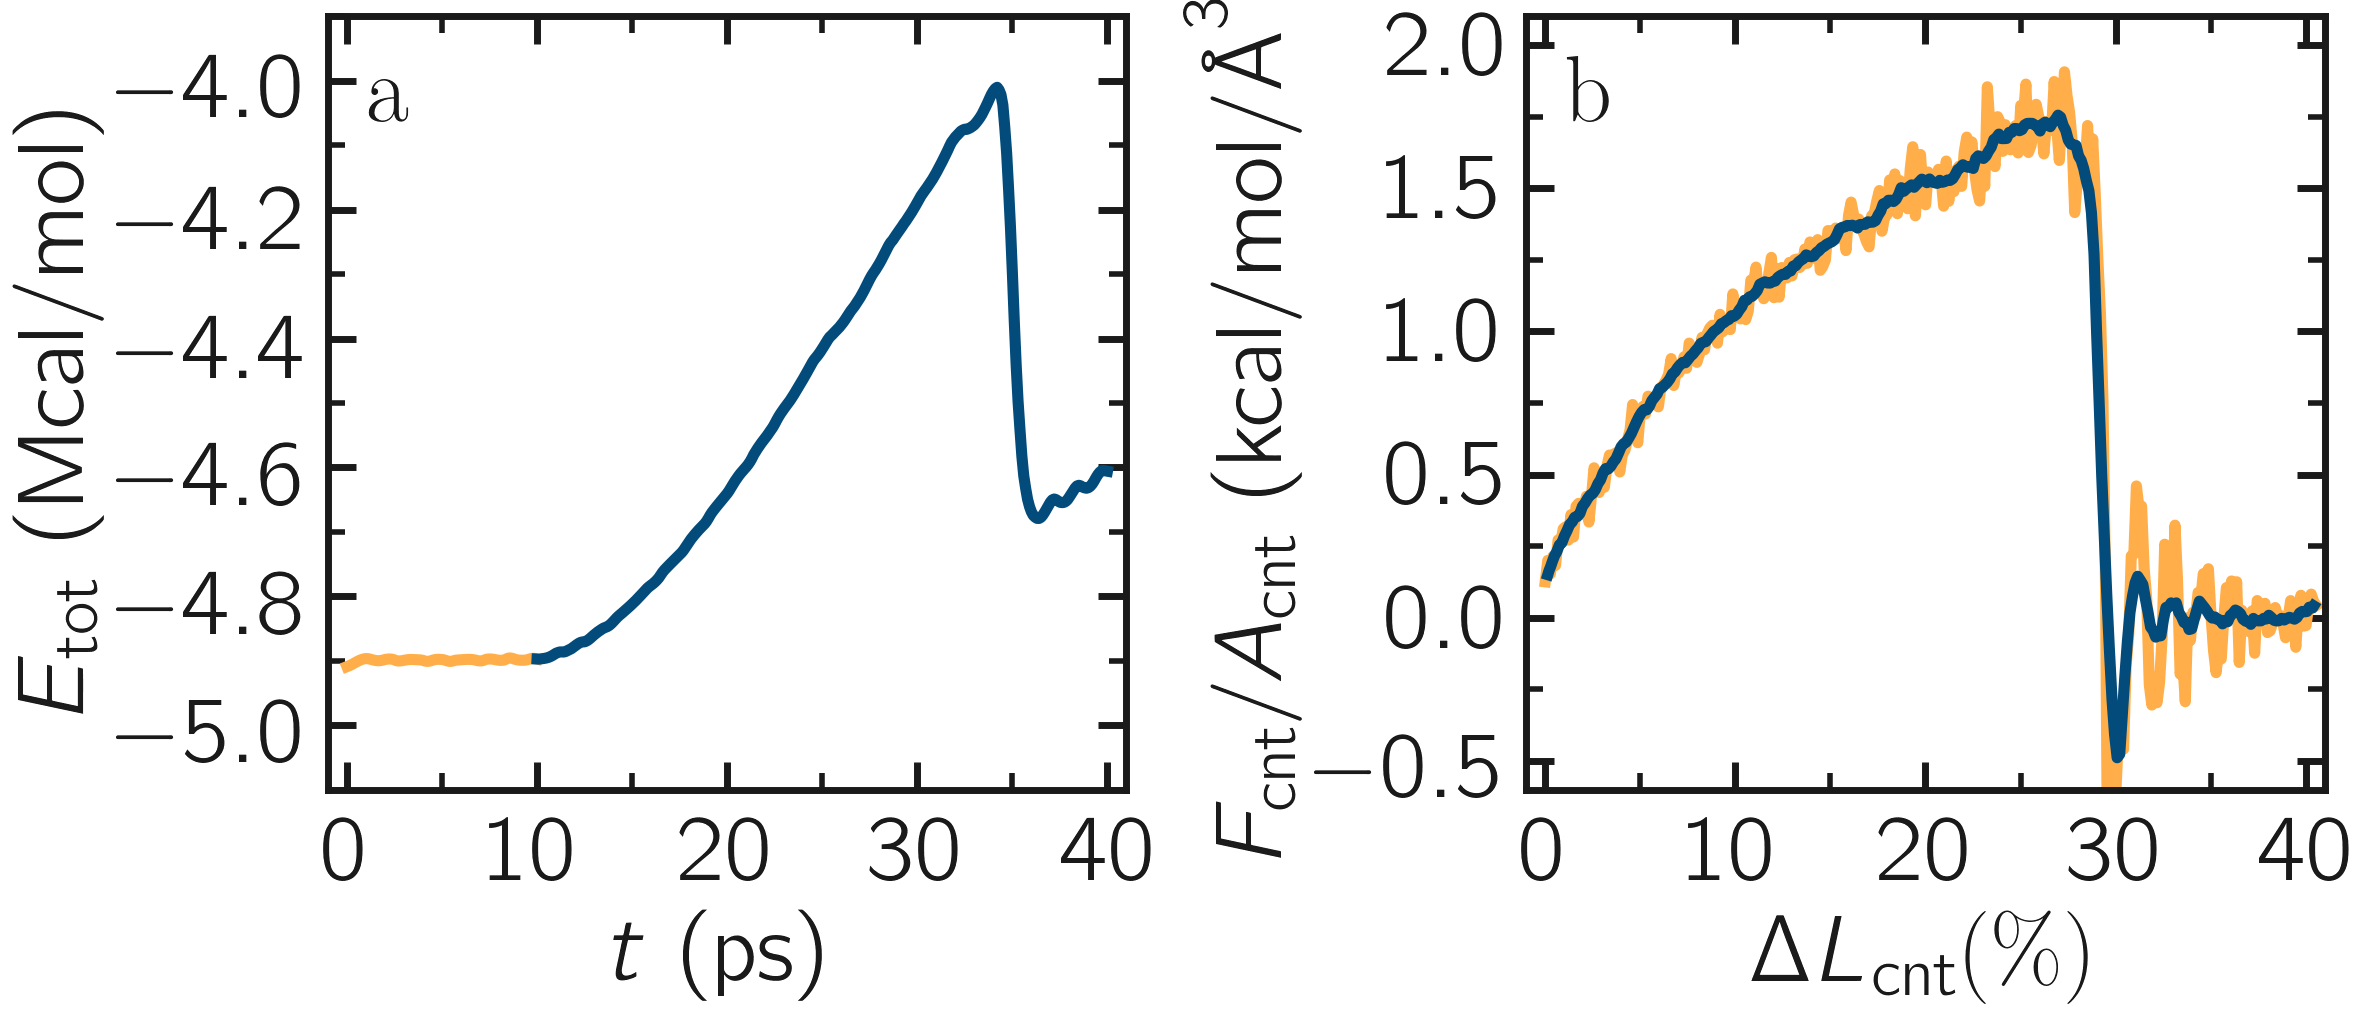
\includegraphics[width=\linewidth]{CNT-breakable-stress-energy}
\caption{a) Evolution of the total energy $E_\text{tot}$ of the CNT with time $t$.
b) Stress applied on the CNT during deformation, $F_\text{cnt}/A_\text{cnt}$,
where $F_\text{cnt}$ is the force and $A_\text{cnt}$ the CNT surface area,
as a function of the strain, $\Delta L_\text{cnt} = (L_\text{cnt}-L_\text{cnt-0}/L_\text{cnt-0})$, where
$L_\text{cnt}$ is the CNT length and $L_\text{cnt-0}$ the CNT initial length,
as simulated during \hyperref[carbon-nanotube-label]{Tutorial 2}.
Here, the potential is AIREBO, and the CNT is breakable.}
\label{fig:CNT-breakable-energy-stress}
\end{figure}

\paragraph{Tip: bonds representation with AIREBO}

In the input file
% do not wrap this line
\href{\filepath tutorial2/solution/breakable-with-tip.lmp}{\dwlcmd{solution/breakable-with-tip.lmp}},
% do not wrap this line
which is an alternate solution for \flecmd{breakable.lmp}, a trick is
used to represent bonds while using AIREBO.  A detailed explanation of
the script is beyond the scope of the present tutorial.  In short, the
trick is to use AIREBO with the \lmpcmd{molecular} atom style, and use
the \lmpcmd{fix bond/break} and \lmpcmd{fix bond/create/angle} commands
to update the status of the bonds during the simulation:
\begin{lstlisting}
fix break all bond/break 1000 1 2.5
fix form all bond/create/angle 1000 1 1 2.0 1 aconstrain 90.0 180
\end{lstlisting}

This ``hack'' works because AIREBO does not pay any attention to bonded
interactions and computes the bond topology dynamically inside the pair
style.  Thus adding bonds of bond style \lmpcmd{zero} does not add any
interactions but allow the visualization of them with \lmpcmd{dump
  image}.  It is, however needed to change the \lmpcmd{special\_bonds}
setting to disable any neighbor list exclusions as they are common for
force fields with explicit bonds.
\begin{lstlisting}
bond_style zero
bond_coeff 1 1.4
special_bonds lj/coul 1.0 1.0 1.0
\end{lstlisting}

% S.G.: we could write a bit more about it

\subsection{Tutorial 3: Polymer in water}
\label{all-atom-label}

\begin{figure}
\centering
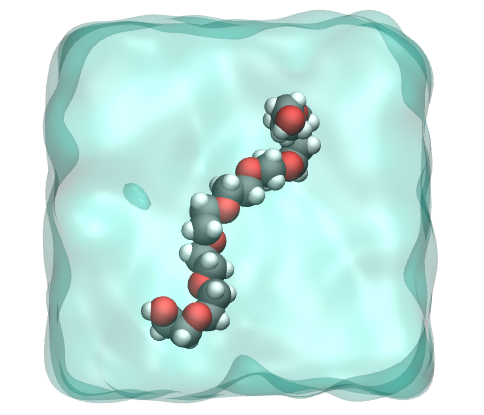
\includegraphics[width=0.55\linewidth]{PEG}
\caption{The polymer molecule (PEG - PolyEthylene Glycol) solvated in water as
simulated during \hyperref[all-atom-label]{Tutorial 3}.  Water molecules are
represented as a transparent continuum field for clarity.}
\label{fig:PEG}
\end{figure}

\noindent The goal of this tutorial is to use LAMMPS to solvate a small hydrophilic
polymer (PEG - PolyEthylene Glycol) in a reservoir of water (Fig.~\ref{fig:PEG}).
Once the water reservoir is properly equilibrated at the desired temperature and
pressure, the polymer molecule is added and a constant stretching force is applied
to both ends of the polymer.  The evolution of the polymer length is measured as
a function of time.  The GROMOS 54A7 force field~\cite{schmid2011definition} is used
for the PEG, the SPC/Fw model~\cite{wu2006flexible} is used for the water, and the
long-range Coulomb interactions are solved using the PPPM solver~\cite{luty1996calculating}.
This tutorial was inspired by a publication by Liese and coworkers, in which molecular
dynamics simulations are compared with force spectroscopy experiments, see Ref.\,~\citenum{liese2017hydration}.

\subsubsection{Preparing the water reservoir}

In this tutorial, the water reservoir is first prepared in the absence of the polymer.
A rectangular box of water is created and equilibrated at ambient temperature and
pressure.  The SPC/Fw water model is used~\cite{wu2006flexible}, which is
a flexible variant of the rigid SPC (simple point charge) model~\cite{berendsen1981interaction}.
To set up this tutorial, select \guicmd{Start Tutorial 3} from the
\guicmd{Tutorials} menu of \lammpsgui{} and follow the instructions.
The editor should display the following content corresponding to \flecmd{water.lmp}:
\begin{lstlisting}
units real
atom_style full
bond_style harmonic
angle_style harmonic
dihedral_style harmonic
pair_style lj/cut/coul/long 10
kspace_style ewald 1e-5
special_bonds lj 0.0 0.0 0.5 coul 0.0 0.0 1.0 angle yes
\end{lstlisting}
With the unit style \lmpcmd{real}, masses are in grams per mole, distances in
Ångströms, time in femtoseconds, and energies in kcal/mole.  With the \lmpcmd{atom\_style full},
each atom is a dot with a mass and a charge that can be linked by bonds, angles,
dihedrals, and/or impropers.  The \lmpcmd{bond\_style},
\lmpcmd{angle\_style}, and \lmpcmd{dihedral\_style} commands define the potentials
for the bonds, angles, and dihedrals used in the simulation, here \lmpcmd{harmonic}.
With the \lmpcmd{pair\_style} named \lmpcmd{lj/cut/coul/long}, atoms interact through
both a Lennard-Jones (LJ) potential and Coulomb interactions.  The value of $10\,\text{\AA{}}$ is the cutoff,
and the \lmpcmd{ewald} command defines the long-range solver for the Coulomb
interactions~\cite{ewald1921berechnung}.  Finally, the \lmpcmd{special\_bonds} command, which was already seen in
\hyperref[carbon-nanotube-label]{tutorial 2}, sets the LJ and Coulomb weighting
factors for the interaction between neighboring atoms.

Let us create a 3D simulation box of dimensions $6 \times 3 \times 3 \; \text{nm}^3$,
and make space for 8 atom types (2 for the water, 6 for the polymer), 7 bond types
(1 for the water, 6 for the polymer), 8 angle types (1 for the water, 7 for the polymer),
and 4 dihedral types (only for the polymer).  Copy the following lines into \flecmd{water.lmp}:
\begin{lstlisting}
 region box block -30 30 -15 15 -15 15
 create_box 8 box &
 bond/types 7 &
 angle/types 8 &
 dihedral/types 4 &
 extra/bond/per/atom 3 &
 extra/angle/per/atom 6 &
 extra/dihedral/per/atom 10 &
 extra/special/per/atom 14
\end{lstlisting}
The \lmpcmd{extra/x/per/atom} commands are here for
memory allocation.  We will use a file named
\href{\filepath tutorial3/parameters.inc}{\dwlcmd{parameters.inc}} that contains
all the parameters (masses, interaction energies, bond equilibrium
distances, etc).  In \flecmd{water.lmp}, add the following line:
\begin{lstlisting}
include parameters.inc
\end{lstlisting}

\begin{note}
This tutorial uses type labels~\cite{typelabel_paper} to map each of the
numeric atom types with a string (see the \flecmd{parameters.inc} file):
\lmpcmdnote{labelmap atom 1 OE 2 C 3 HC 4 H 5 CPos 6 OAlc 7 OW 8 HW}
Therefore, the oxygen and hydrogen atoms of water (respectively types 7 and 8)
can be referred to as `OW' and `HW', respectively.  Similar maps are used for
the bond types, angle types, and dihedral types.
\end{note}

Let us create water molecules.  To do so, let us import a molecule template called
\flecmd{water.mol} and then randomly create 700 molecules.  Add the following
lines into \flecmd{water.lmp}:
\begin{lstlisting}
molecule h2omol water.mol
create_atoms 0 random 700 87910 NULL mol h2omol 454756 &
  overlap 1.0 maxtry 50
\end{lstlisting}
The \lmpcmd{overlap 1.0} option of the \lmpcmd{create\_atoms} command ensures
that no atoms are placed exactly in the same position, as this would cause the
simulation to crash.  The \lmpcmd{maxtry 50} asks LAMMPS to try at most 50 times
to insert the molecules, which is useful in case some insertion attempts are
rejected due to overlap.  In some cases, depending on the system and the values
of \lmpcmd{overlap} and \lmpcmd{maxtry}, LAMMPS may not create the desired number
of molecules.  Always check the number of created atoms in the \lmpcmd{log} file
(or in the \guicmd{Output} window), where you should see:
\begin{lstlisting}
Created 2100 atoms
\end{lstlisting}
When LAMMPS fails to create the desired number of molecules, a WARNING appears.
The molecule template called \href{\filepath tutorial3/water.mol}{\dwlcmd{water.mol}}
must be downloaded and saved next to \flecmd{water.lmp}.  This template contains
the necessary structural information of a water molecule, such as the number of
atoms, or the IDs of the atoms that are connected by bonds and angles.

Then, let us organize the atoms of types OW and HW of the water molecules in a
group named \lmpcmd{H2O} and perform a small energy minimization.  The energy
minimization is mandatory here because of the small \lmpcmd{overlap} value
of 1~Ångstrom chosen in the \lmpcmd{create\_atoms} command.  Add the following lines into \flecmd{water.lmp}:
\begin{lstlisting}
group H2O type OW HW
minimize 1.0e-4 1.0e-6 100 1000
reset_timestep 0
\end{lstlisting}
Resetting the step of the simulation to 0 using the
\lmpcmd{reset\_timestep} command is optional.
It is used here because the number of iterations performed by the \lmpcmd{minimize}
command is usually not a round number, since the minimization stops when one of
four criteria is reached.  We will use \lmpcmd{fix npt} to control the temperature
and pressure of the molecules with a Nosé-Hoover thermostat and barostat,
respectively~\cite{nose1984unified, hoover1985canonical, martyna1994constant}.
Add the following line into \flecmd{water.lmp}:
\begin{lstlisting}
fix mynpt all npt temp 300 300 100 iso 1 1 1000
\end{lstlisting}
The \lmpcmd{fix npt} allows us to impose both a temperature of $300\,\text{K}$
(with a damping constant of $100\,\text{fs}$), and a pressure of 1 atmosphere
(with a damping constant of $1000\,\text{fs}$).  With the \lmpcmd{iso} keyword,
the three dimensions of the box will be re-scaled simultaneously.

Let us output the system into images by adding the following commands to \flecmd{water.lmp}:
\begin{lstlisting}
dump viz all image 250 myimage-*.ppm type type &
  shiny 0.1 box no 0.01 view 0 90 zoom 3 size 1000 600
dump_modify viz backcolor white &
  acolor OW red acolor HW white &
  adiam OW 3 adiam HW 1.5
\end{lstlisting}
Let us also extract the volume and density every 500 steps:
\begin{lstlisting}
variable myvol equal vol
variable myoxy equal count(H2O)/3
variable NA equal 6.022e23
variable Atom equal 1e-10
variable M equal 0.018
variable rho equal ${myoxy}*${M}/(v_myvol*${NA}*${Atom}^3)
thermo 500
thermo_style custom step temp etotal v_myvol v_rho
\end{lstlisting}
Here, several variables are defined and used for converting the units of the
density in kg/mol:  The variable \lmpcmd{myoxy} represents the number of
atoms divided by 3,  which corresponds to the number of molecules, $N_\text{H2O}$,
and the variable \lmpcmd{myrho} is the density in kg/mol:
\begin{equation}
\rho = \dfrac{N_\text{H2O}}{V N_\text{A}},
\end{equation}
where $V$ is the volume in m$^3$, $N_\text{A}$ the Avogadro number, and
$M = 0.018$\,kg/mol the molar mass of water.

Finally, let us set the timestep to 1.0 fs, and run the simulation for 15~ps by
adding the following lines into \flecmd{water.lmp}:
\begin{lstlisting}
timestep 1.0
run 15000

write_restart water.restart
\end{lstlisting}
The final state is saved in a binary file named \flecmd{water.restart}.
Run the input using LAMMPS.  The system reaches its equilibrium temperature
after just a few picoseconds, and its equilibrium density after approximately
10~picoseconds (Fig.~\ref{fig:PEG-density}).  A snapshot of the equilibrated
system can also be seen in Fig.~\ref{fig:PEG-water}.

\begin{figure}
\centering
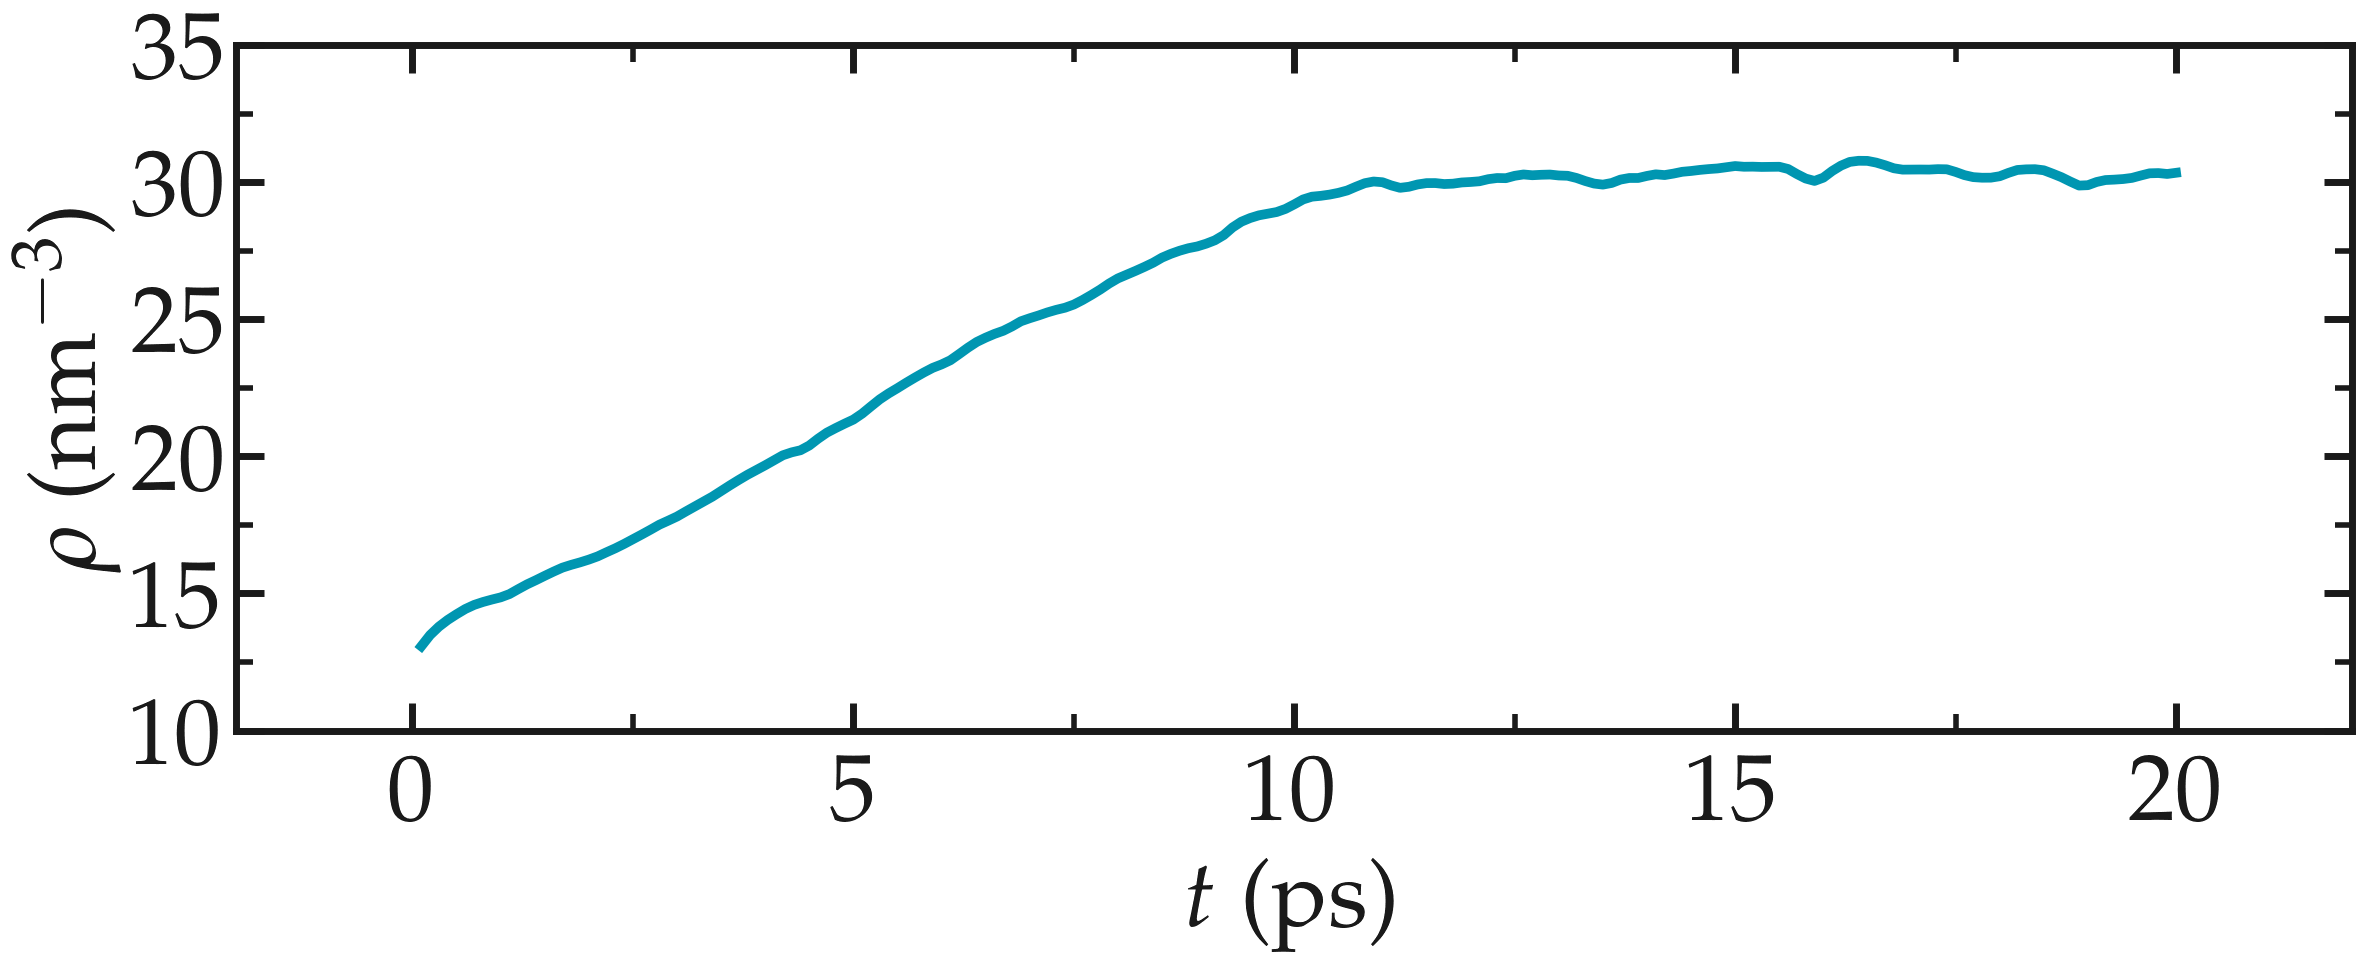
\includegraphics[width=\linewidth]{PEG-density}
\caption{a) Temperature ($T$) of the water reservoir from
\hyperref[all-atom-label]{Tutorial 3} as a function of the ($t$).  The horizontal dashed line is
the target temperature of 300\,K.  b) Evolution of the system density ($\rho$) with $t$.}
\label{fig:PEG-density}
\end{figure}

\begin{note}
The binary file created by the \lmpcmdnote{write\_restart} command contains the
complete state of the simulation, including atomic positions, velocities, and
box dimensions (similar to \lmpcmdnote{write\_data}), but also the groups,
the compute, or the \lmpcmdnote{atom\_style}.  Use the \guicmd{Inspect Restart}
option of the \lammpsgui{} to vizualize the content saved in \flecmd{water.restart}.
\end{note}

\begin{figure}
\centering
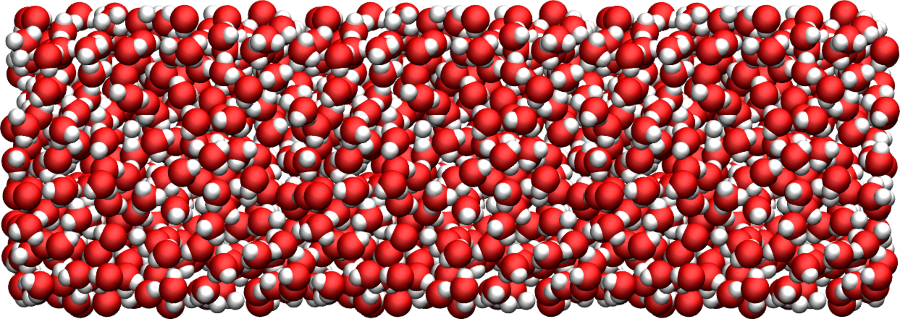
\includegraphics[width=\linewidth]{PEG-water}
\caption{The water reservoir from \hyperref[all-atom-label]{Tutorial 3}
after equilibration.  Oxygen atoms are in red, and hydrogen atoms are in white.}
\label{fig:PEG-water}
\end{figure}

\subsubsection{Solvating the PEG in water}

Now that the water reservoir is equilibrated, we can safely add the PEG polymer
to the water.  The PEG molecule topology was downloaded from the ATB repository
\cite{malde2011automated, oostenbrink2004biomolecular}.  It has a formula
$\text{C}_{16}\text{H}_{34}\text{O}_{9}$, and the parameters are taken from
the GROMOS 54A7 force field~\cite{schmid2011definition} (Fig.~\ref{fig:PEG-in-vacuum}).

\begin{figure}
\centering
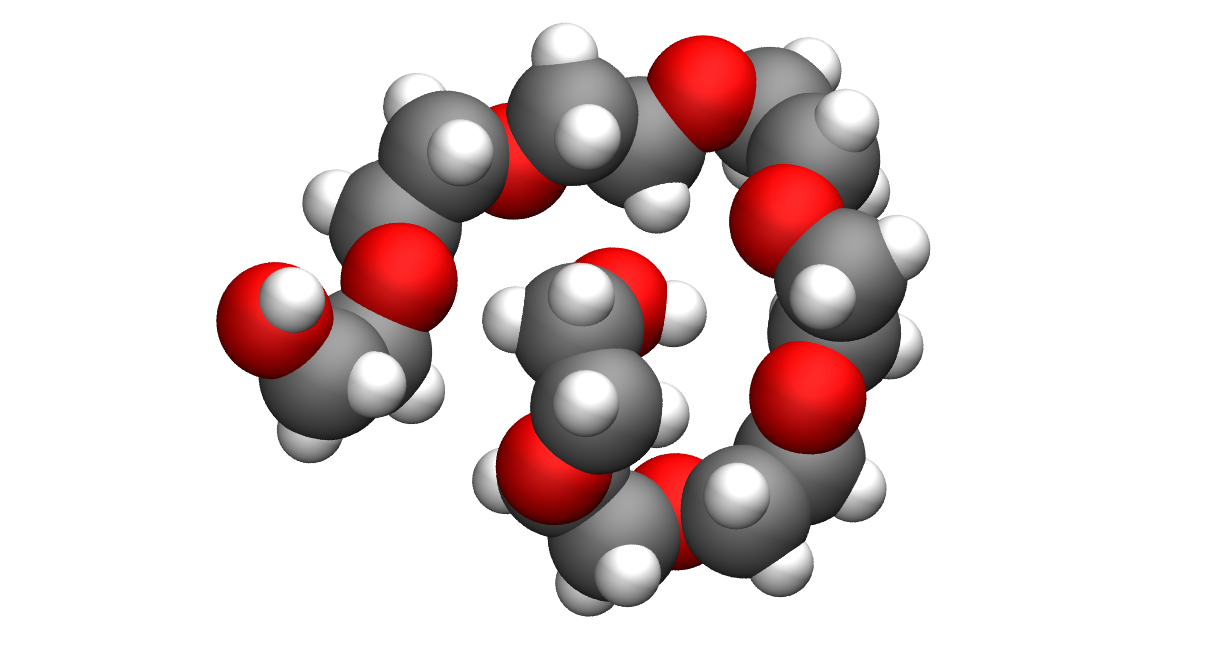
\includegraphics[width=0.8\linewidth]{PEG-in-vacuum}
\caption{The PEG molecule from \hyperref[all-atom-label]{Tutorial 3}.
The carbon atoms are in gray, the oxygen atoms in red, and the hydrogen atoms in white.}
\label{fig:PEG-in-vacuum}
\end{figure}

Open the file named \flecmd{merge.lmp} that was downloaded
alongside \flecmd{water.lmp} during the tutorial setup.  It only contain one line:
\begin{lstlisting}
read_restart water.restart
\end{lstlisting}
Most of the commands that were initially present in \flecmd{water.lmp}, such as
the \lmpcmd{units} of the \lmpcmd{atom\_style} commands do not need to be repeated,
as they were saved within the \flecmd{.restart} file.  There is also no need to
re-include the parameters from the \flecmd{.inc} file.  The \lmpcmd{kspace\_style}
command, however, is not saved by the \lmpcmd{write\_restart} command and must be
repeated.  Since Ewald summation is not the most efficient choice for such dense
system, let us use PPPM (for particle-particle particle-mesh) for the rest
of the tutorial.  Add the following command to \flecmd{merge.lmp}:
\begin{lstlisting}
kspace_style pppm 1e-5
\end{lstlisting}

Using the molecule template for the polymer called
\href{\filepath tutorial3/peg.mol}{\dwlcmd{peg.mol}},
let us create a single molecule in the middle of the box by adding the following
commands to \flecmd{merge.lmp}:
\begin{lstlisting}
molecule pegmol peg.mol
create_atoms 0 single 0 0 0 mol pegmol 454756
\end{lstlisting}
Let us create a group for the atoms of the PEG (the previously created
group H2O was saved by the restart and can be omitted):
\begin{lstlisting}
group PEG type C CPos H HC OAlc OE
\end{lstlisting}
Water molecules that are overlapping with the PEG must be deleted to avoid future
crashing.  Add the following line into \flecmd{merge.lmp}:
\begin{lstlisting}
delete_atoms overlap 2.0 H2O PEG mol yes
\end{lstlisting}
Here the value of 2.0~Ångströms for the overlap cutoff was fixed arbitrarily and can
be chosen through trial and error.  If the cutoff is too small, the simulation will
crash because atoms that are too close to each other undergo forces
that can be extremely large.  If the cutoff is too large, too many water
molecules will unnecessarily be deleted.

Let us use the \lmpcmd{fix npt} to control the temperature, as
well as the pressure by allowing the box size to be rescaled along the $x$-axis:
\begin{lstlisting}
fix mynpt all npt temp 300 300 100 x 1 1 1000
\end{lstlisting}
Let us also use the \lmpcmd{recenter} command to always keep the PEG at
the position $(0,~0,~0)$:
\begin{lstlisting}
fix myrct PEG recenter 0 0 0 shift all
\end{lstlisting}
Note that the \lmpcmd{recenter} command has no impact on the dynamics,
it simply ensures that the system does not drift, which can be more practical for visualizing and analyzing the system

Let us create images of the systems:
\begin{lstlisting}
dump viz all image 250 myimage-*.ppm type &
  type shiny 0.1 box no 0.01 &
  view 0 90 zoom 3.3 fsaa yes bond atom 0.8 size 1100 600
dump_modify viz backcolor white &
  acolor OW red acolor HW white &
  acolor OE darkred acolor OAlc darkred &
  acolor C gray acolor CPos gray &
  acolor H white acolor HC white &
  adiam OW 0.2 adiam HW 0.2 &
  adiam C 2.8 adiam CPos 2.8 adiam OAlc 2.6 &
  adiam H 1.4 adiam HC 1.4 adiam OE 2.6
thermo 500
\end{lstlisting}
Finally, let us perform a short equilibration and save the
final state to a \lmpcmd{.restart} file.  Add the following lines to the data file:
\begin{lstlisting}
timestep 1.0
run 10000

write_restart merge.restart
\end{lstlisting}
Run the simulation using LAMMPS.  From the outputs, you can make
sure that the temperature remains close to the
target value of $300~\text{K}$ throughout the entire simulation, and that
the volume and total energy are almost constant, indicating
that the system was in a reasonable configuration from the start.
See a snapshot of the system in Fig.~\ref{fig:PEG-solvated}.

\begin{figure}
\centering
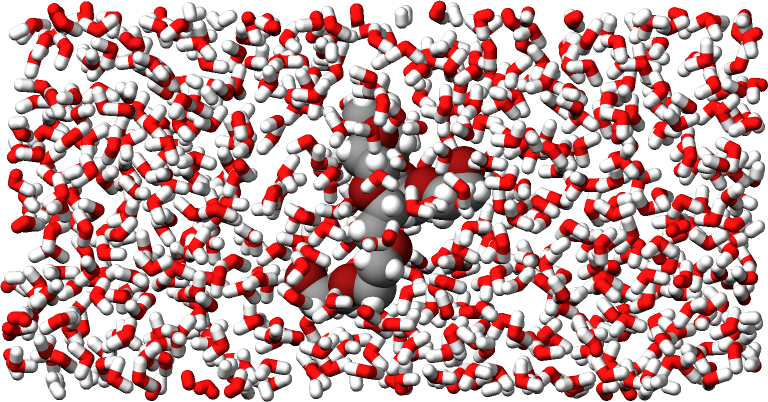
\includegraphics[width=\linewidth]{PEG-solvated}
\caption{The PEG molecule solvated in water as simulated during
\hyperref[all-atom-label]{Tutorial 3}.}
\label{fig:PEG-solvated}
\end{figure}

\subsubsection{Stretching the PEG molecule}

Here, a constant force is applied to both ends of the PEG molecule until it
stretches.  Open the file named \flecmd{pull.lmp}, which
only contains two lines:
\begin{lstlisting}
kspace_style pppm 1e-5
read_restart merge.restart
\end{lstlisting}
Next, we'll create new atom groups, each containing a single oxygen atom.  The atoms of type OAlc
correspond to the hydroxyl (alcohol) group oxygen atoms located at the ends
of the PEG molecule, which we will use to apply the force.  Add the
following lines to \flecmd{pull.lmp}:
\begin{lstlisting}
group ends type OAlc
variable xcm equal xcm(ends,x)
variable oxies atom type==label2type(atom,OAlc)
variable end1 atom v_oxies*(x>v_xcm)
variable end2 atom v_oxies*(x<v_xcm)
group topull1 variable end1
group topull2 variable end2
\end{lstlisting}
These lines identify the oxygen atoms (type OAlc) at the ends of the PEG
molecule and calculates their center of mass along the $x$-axis.  It then
divides these atoms into two groups, \lmpcmd{end1} (i.e.,~the OAlc atom to
the right of the center) and \lmpcmd{end2} (i.e.,~the OAlc atom to the right
of the center), for applying force during the stretching process.

Add the following \lmpcmd{dump} command to create images of the system:
\begin{lstlisting}
dump viz all image 250 myimage-*.ppm type &
  type shiny 0.1 box no 0.01 &
  view 0 90 zoom 3.3 fsaa yes bond atom 0.8 size 1100 600
dump_modify viz backcolor white &
  acolor OW red acolor HW white &
  acolor OE darkred acolor OAlc darkred &
  acolor C gray acolor CPos gray &
  acolor H white acolor HC white &
  adiam OW 0.2 adiam HW 0.2 &
  adiam C 2.8 adiam CPos 2.8 adiam OAlc 2.6 &
  adiam H 1.4 adiam HC 1.4 adiam OE 2.6
\end{lstlisting}
Let us use a single Nosé-Hoover thermostat applied to all the atoms,
and let us keep the PEG in the center of the box, by adding
the following lines to \flecmd{pull.lmp}:
\begin{lstlisting}
timestep 1.0
fix mynvt all nvt temp 300 300 100
fix myrct PEG recenter 0 0 0 shift all
\end{lstlisting}

To investigate the stretching of the PEG molecule, let us compute its radius of
gyration~\cite{fixmanRadiusGyrationPolymer1962a} and the angles of its dihedral
constraints using the following commands:
\begin{lstlisting}
compute rgyr PEG gyration
compute prop PEG property/local dtype
compute dphi PEG dihedral/local phi
\end{lstlisting}
The radius of gyration can be directly printed with the \lmpcmd{thermo\_style} command:
\begin{lstlisting}
thermo_style custom step temp etotal c_rgyr
thermo 250
dump mydmp all local 100 pull.dat index c_dphi c_prop
\end{lstlisting}
By contrast with the radius of gyration (compute \lmpcmd{rgyr}), the dihedral angle  % SG: why is c_prop not printed?
$\phi$ (compute \lmpcmd{dphi}) is returned as a vector by the \lmpcmd{compute dihedral/local}
command and must be written to a file using the \lmpcmd{dump local} command.

Finally, let us simulate 15 picoseconds without any external force:
\begin{lstlisting}
run 15000
\end{lstlisting}
This initial run will serve as a benchmark to quantify the changes caused by
the applied force in later steps.  Next, let us apply a force to the two selected
oxygen atoms using two \lmpcmd{addforce} commands, and then run the simulation
for an extra 15~ps:
\begin{lstlisting}
fix myaf1 topull1 addforce 10 0 0
fix myaf2 topull2 addforce -10 0 0
run 15000
\end{lstlisting}
Each applied force has a magnitude of $10\,\text{kcal/mol/\AA{}}$, corresponding to $0.67\,\text{nN}$.
This value was chosen to be sufficiently large to overcome both the thermal agitation and
the entropic contributions from the molecules.

Run the \flecmd{pull.lmp} file using LAMMPS.  From the generated images of the system,
you should observe that the PEG molecule eventually aligns
in the direction of the applied force (as seen in Fig.~\ref{fig:PEG-in-water}).
The evolutions of the radius of gyration over
time indicates that the PEG quickly adjusts to the external force
(Fig.~\ref{fig:PEG-distance}\,a).  Additionally, from the values of the dihedral angles
printed in the \flecmd{pull.dat} file, you can create a histogram
of dihedral angles for a specific type.  For example, the angle $\phi$ for dihedrals
of type 1 (C-C-OE-C) is shown in Fig.~\ref{fig:PEG-distance}\,b.

\begin{figure}
\centering
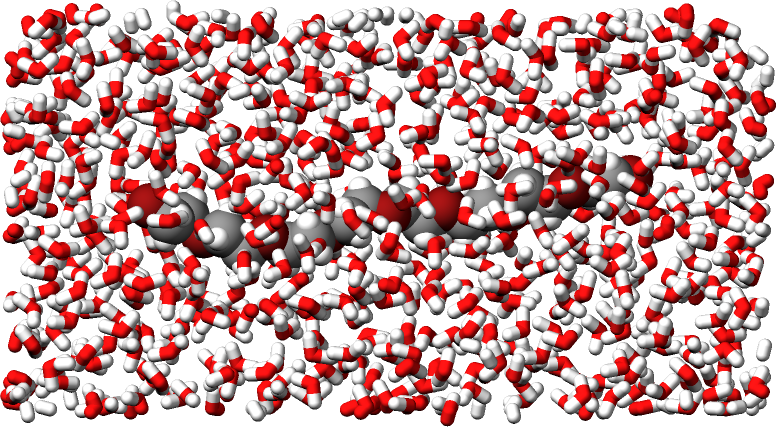
\includegraphics[width=\linewidth]{PEG-in-water}
\caption{PEG molecule stretched along the $x$ direction in water
as simulated during \hyperref[all-atom-label]{Tutorial 3}.}
\label{fig:PEG-in-water}
\end{figure}

\begin{figure}
\centering
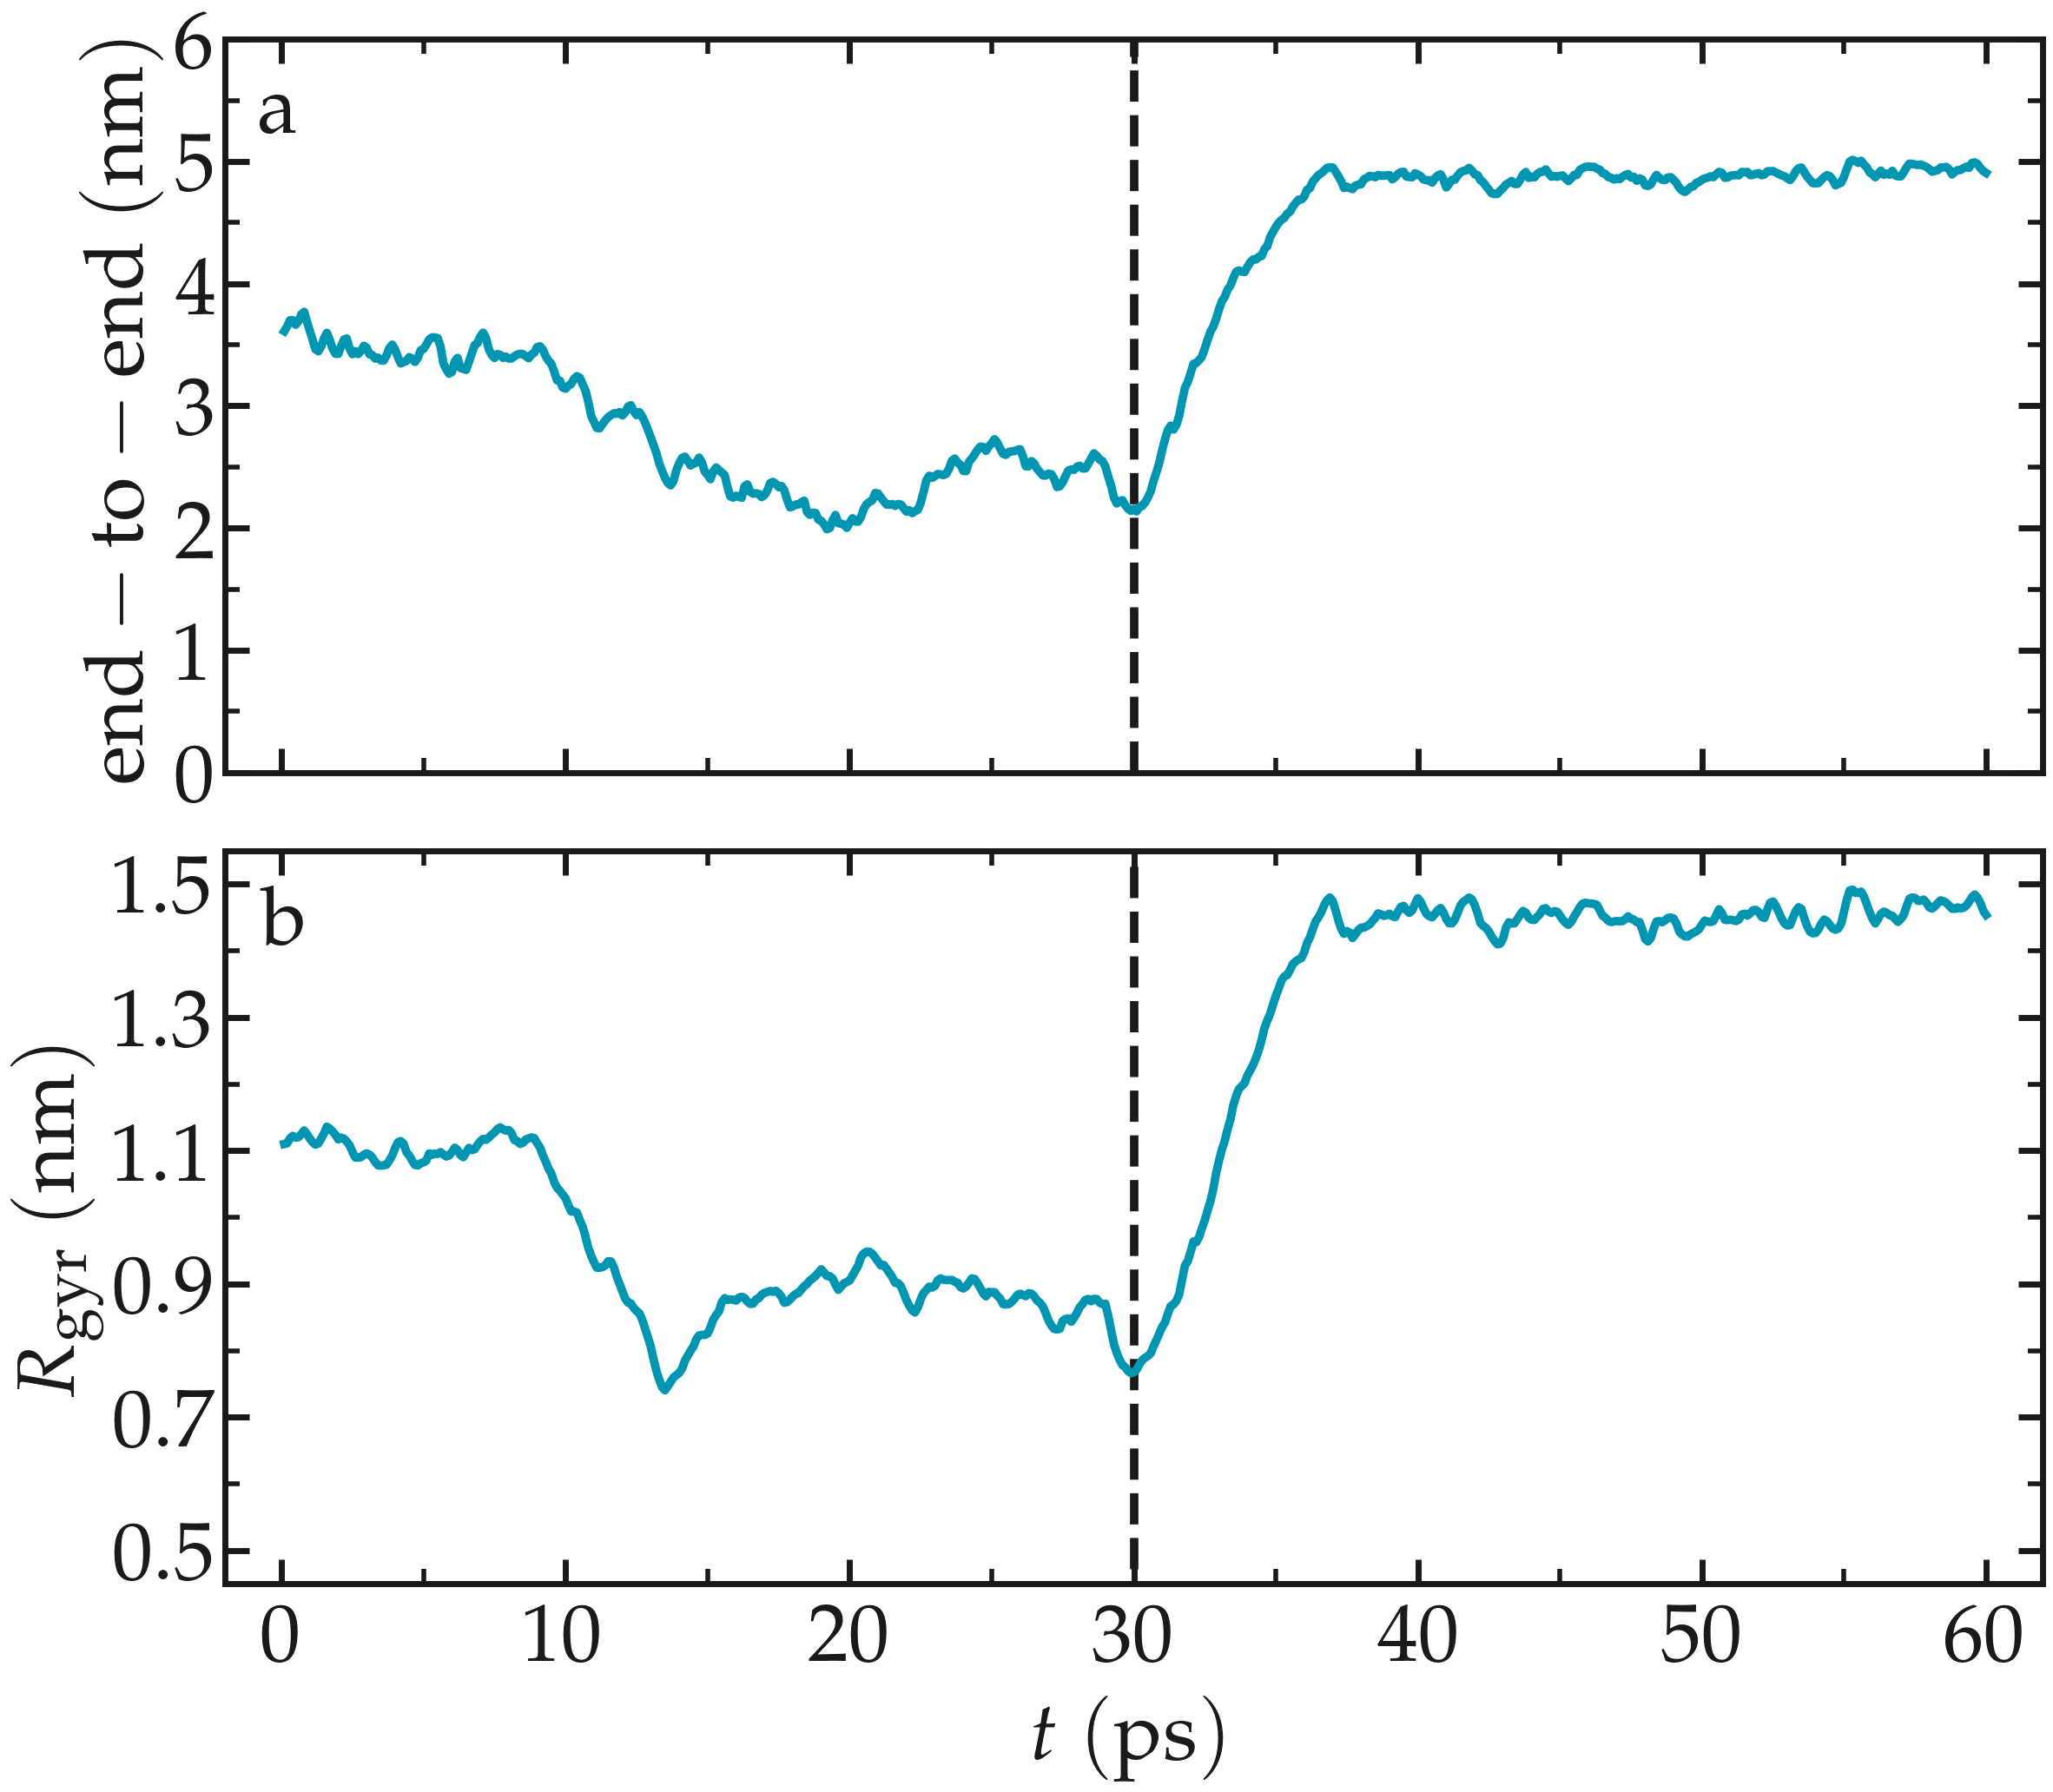
\includegraphics[width=\linewidth]{PEG-distance}
\caption{a) Evolution of
the radius of gyration $R_\text{gyr}$ of the PEG molecule
from \hyperref[all-atom-label]{Tutorial 3}, with the force
applied starting at $t = 15\,\text{ps}$.  b) Histograms of the dihedral angles of type 1
in the absence (orange) and in the presence (blue) of the applied force.}
\label{fig:PEG-distance}
\end{figure}

\subsection{Tutorial 4: Nanosheared electrolyte}
\label{sheared-confined-label}

\begin{figure}
\centering
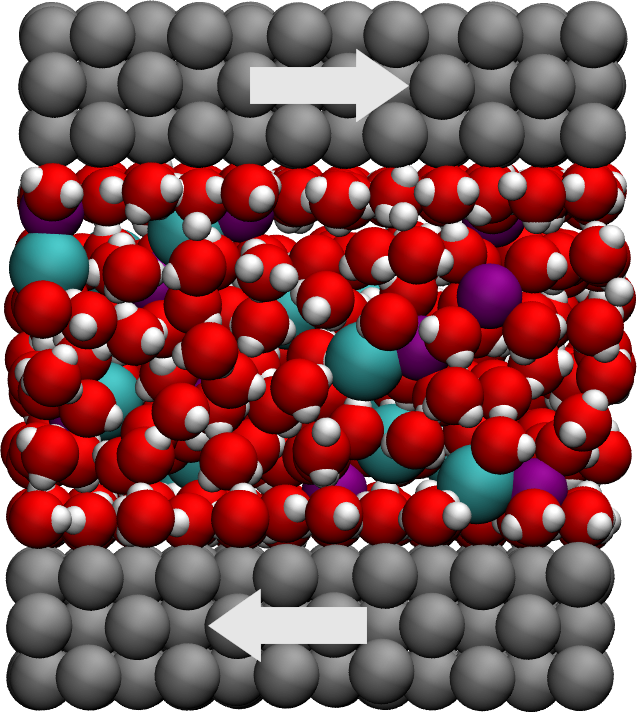
\includegraphics[width=0.55\linewidth]{NANOSHEAR}
\caption{The electrolyte confined in a nanometer slit pore as simulated during
\hyperref[sheared-confined-label]{Tutorial 4}.  $\text{Na}^+$ ions are represented
as purple spheres, $\text{Cl}^-$ ions as cyan spheres, water molecules are colored
in red and white, and the walls are colored in gray.  The arrows indicate the
imposed lateral motion of the walls.}
\label{fig:NANOSHEAR}
\end{figure}

\noindent The objective of this tutorial is to simulate an electrolyte
nanoconfined and sheared between two walls (Fig.~\ref{fig:NANOSHEAR}).  The density
and velocity profiles of the fluid in the direction normal to the walls are
extracted to highlight the effect of confining a fluid on its local properties.
This tutorial demonstrates key concepts of combining a fluid and a solid in
the same simulation.  A major difference from the previous tutorial,
\hyperref[all-atom-label]{Polymer in water}, is that here a rigid four-point
water model named TIP4P/2005 is used~\cite{abascal2005general}.

\begin{note}
Four-point water models such as TIP4P/2005 are widely used as they offer a
good compromise between accuracy and computational cost~\cite{kadaoluwa2021systematic}.
\end{note}

\subsubsection{System preparation}

The fluid and walls must first be generated, followed by equilibration at the
desired temperature and pressure.

\paragraph{System generation}

To set up this tutorial, select \guicmd{Start Tutorial 4} from the
\guicmd{Tutorials} menu of \lammpsgui{} and follow the instructions.
The editor should display the following content corresponding to \flecmd{create.lmp}:
\begin{lstlisting}
boundary p p f
units real
atom_style full
bond_style harmonic
angle_style harmonic
pair_style lj/cut/tip4p/long O H O-H H-O-H 0.1546 12.0
kspace_style pppm/tip4p 1.0e-5
kspace_modify slab 3.0
\end{lstlisting}
These lines are used to define the most basic parameters, including the
atom, bond, and angle styles, as well as interaction
potential.  Here, \lmpcmd{lj/cut/tip4p/long} imposes a Lennard-Jones potential with
a cut-off at $12\,\text{$\text{\AA{}}$}$ and a long-range Coulomb potential.

So far, the commands are relatively similar to those in the previous tutorial,
\hyperref[all-atom-label]{Polymer in water}, with two major differences: the use
of \lmpcmd{lj/cut/tip4p/long} instead of \lmpcmd{lj/cut/coul/long}, and \lmpcmd{pppm/tip4p}
instead of \lmpcmd{pppm}.  When using \lmpcmd{lj/cut/tip4p/long} and \lmpcmd{pppm/tip4p},
the interactions resemble the conventional Lennard-Jones and Coulomb interactions,
except that they are specifically designed for the four-point water model.  As a result,
LAMMPS automatically creates a four-point water molecule, assigning type O
atoms as oxygen and type H atoms as hydrogen.  The fourth massless atom (M) of the
TIP4P water molecule does not have to be defined explicitly, and the value of
$0.1546\,\text{$\text{\AA{}}$}$ corresponds to the O-M distance of the
TIP4P-2005 water model~\cite{abascal2005general}.  All other atoms in the simulation
are treated as usual, with long-range Coulomb interactions.  Another novelty, here, is
the use of \lmpcmd{kspace\_modify slab 3.0} that is combined with the non-periodic
boundaries along the $z$ coordinate: \lmpcmd{boundary p p f}.  With the \lmpcmd{slab}
option, the system is treated as periodical along $z$, but with an empty volume inserted
between the periodic images of the slab, and the interactions along $z$ effectively turned off.

Let us create the box and the label maps by adding the following lines to \flecmd{create.lmp}:
\begin{lstlisting}
lattice fcc 4.04
region box block -3 3 -3 3 -5 5
create_box 5 box bond/types 1 angle/types 1 &
  extra/bond/per/atom 2 extra/angle/per/atom 1 &
  extra/special/per/atom 2
labelmap atom 1 O 2 H 3 Na+ 4 Cl- 5 WALL
labelmap bond 1 O-H
labelmap angle 1 H-O-H
\end{lstlisting}
The \lmpcmd{lattice} command defines the unit cell.  Here, the face-centered cubic (fcc) lattice
with a scale factor of 4.04 has been chosen for the future positioning of the atoms
of the walls.  The \lmpcmd{region} command defines a geometric region of space.  By choosing
$\text{xlo}=-3$ and $\text{xlo}=3$, and because we have previously chosen a lattice with a scale
factor of 4.04, the region box extends from $-12.12~\text{\AA{}}$ to $12.12~\text{\AA{}}$
along the $x$ direction.  The \lmpcmd{create\_box} command creates a simulation box with
5 types of atoms: the oxygen and hydrogen of the water molecules, the two ions ($\text{Na}^+$,
$\text{Cl}^-$), and the atoms from the walls.  The simulation contains 1 type of bond
and 1 type of angle (both required by the water molecules).
The parameters for these bond and angle constraints will be given later.  The \lmpcmd{extra/ (...)}
keywords are for memory allocation.  Finally, the \lmpcmd{labelmap} commands assign
alphanumeric type labels to each numeric atom type, bond type, and angle type.

Now, we can add atoms to the system.  First, let us create two sub-regions corresponding
respectively to the two solid walls, and create a larger region from the union of the
two regions.  Then, let us create atoms of type WALL within the two regions.  Add the
following lines to \flecmd{create.lmp}:
\begin{lstlisting}
region rbotwall block -3 3 -3 3 -4 -3
region rtopwall block -3 3 -3 3 3 4
region rwall union 2 rbotwall rtopwall
create_atoms WALL region rwall
\end{lstlisting}
Atoms will be placed in the positions of the previously defined lattice, thus
forming fcc solids.

To add the water molecules, the molecule
template called \href{\filepath tutorial4/water.mol}{\dwlcmd{water.mol}}
must be located next to \flecmd{create.lmp}.  The template contains all the
necessary information concerning the water molecule, such as atom positions,
bonds, and angles.  Add the following lines to \flecmd{create.lmp}:
\begin{lstlisting}
region rliquid block INF INF INF INF -2 2
molecule h2omol water.mol
create_atoms 0 region rliquid mol h2omol 482793
\end{lstlisting}
Within the last three lines, a \lmpcmd{region} named \lmpcmd{rliquid} is
created based on the last defined lattice, \lmpcmd{fcc 4.04}.  \lmpcmd{rliquid}
will be used for depositing the water molecules.  The \lmpcmd{molecule} command
opens up the molecule template called \flecmd{water.mol}, and names the
associated molecule \lmpcmd{h2omol}.  The new molecules are placed on the
\lmpcmd{fcc 4.04} lattice by the \lmpcmd{create\_atoms} command.  The first
parameter is 0, meaning that the atom IDs from the \flecmd{water.mol} file
will be used.  The number \lmpcmd{482793} is a seed that is required by LAMMPS,
it can be any positive integer.

Finally, let us create 30 ions (15 $\text{Na}^+$ and 15 $\text{Cl}^-$) in between
the water molecules, by adding the following commands to \flecmd{create.lmp}:
\begin{lstlisting}
create_atoms Na+ random 15 5802 rliquid overlap 0.3 maxtry 500
create_atoms Cl- random 15 9012 rliquid overlap 0.3 maxtry 500
set type Na+ charge 1
set type Cl- charge -1
\end{lstlisting}
Each \lmpcmd{create\_atoms} command will add 15 ions at random positions
within the \lmpcmd{rliquid} region, ensuring that there is no \lmpcmd{overlap}
with existing molecules.  Feel free to increase or decrease the salt concentration
by changing the number of desired ions.  To keep the system charge neutral,
always insert the same number of $\text{Na}^+$ and $\text{Cl}^-$, unless there
are other charges in the system.  The charges of the newly added ions are specified
by the two \lmpcmd{set} commands.

Before starting the simulation, we need to define the parameters of the
simulation: the mass of the 5 atom types (O, H, $\text{Na}^+$, $\text{Cl}^-$,
and wall), the pairwise interaction parameters (in this case, for the
Lennard-Jones potential), and the bond and angle parameters.  Copy the following
lines into \flecmd{create.lmp}:
\begin{lstlisting}
include parameters.inc
include groups.inc
\end{lstlisting}
Both \href{\filepath tutorial4/parameters.inc}{\dwlcmd{parameters.inc}}
and \href{\filepath tutorial4/groups.inc}{\dwlcmd{groups.inc}} files
must be located next to \flecmd{create.lmp}.

The \flecmd{parameters.inc} file contains the masses, as follows:
\begin{lstlisting}
mass O 15.9994
mass H 1.008
mass Na+ 22.990
mass Cl- 35.453
mass WALL 26.9815
\end{lstlisting}
Each \lmpcmd{mass} command assigns a mass in grams/mole to an atom type.
The \flecmd{parameters.inc} file also contains the pair coefficients:
\begin{lstlisting}
pair_coeff O O 0.185199 3.1589
pair_coeff H H 0.0 1.0
pair_coeff Na+ Na+ 0.04690 2.4299
pair_coeff Cl- Cl- 0.1500 4.04470
pair_coeff WALL WALL 11.697 2.574
pair_coeff O WALL 0.4 2.86645
\end{lstlisting}
Each \lmpcmd{pair\_coeff} assigns the depth of the LJ potential
(in kcal/mole), and the distance (in Ångstroms) at which the particle-particle
potential energy is 0.  As noted in previous tutorials, with the important exception of
\lmpcmd{pair\_coeff O WALL}, pairwise interactions were only assigned between
atoms of identical types.  By default, LAMMPS calculates the pair coefficients for the
interactions between atoms of different types (i and j) by using geometric average:
$\epsilon_{ij} = (\epsilon_{ii} + \epsilon_{jj})/2$,  $\sigma_{ij} = (\sigma_{ii} + \sigma_{jj})/2$.
However, if the default value of $5.941\,\text{kcal/mol}$ was used for $\epsilon_\text{1-5}$, the solid
walls would be extremely hydrophilic, causing the water molecules to form dense layers.  As a
comparison, the water-water energy $\epsilon_\text{1-1}$ is only $0.185199\,\text{kcal/mol}$.
Therefore, to make the walls less hydrophilic, the value of $\epsilon_\text{O-WALL}$
was reduced.

Finally, the \flecmd{parameters.inc} file contains the following two lines:
\begin{lstlisting}
bond_coeff O-H 0 0.9572
angle_coeff H-O-H 0 104.52
\end{lstlisting}
The \lmpcmd{bond\_coeff} command, used here for the O-H bond of the water
molecule, sets both the spring constant of the harmonic potential and the
equilibrium bond distance of $0.9572~\text{\AA{}}$.  The constant can be 0 for a
rigid water molecule because the SHAKE algorithm will maintain the rigid
structure of the water molecule (see below)~\cite{ryckaert1977numerical, andersen1983rattle}.
Similarly, the \lmpcmd{angle\_coeff} command for the H-O-H angle of the water molecule sets
the force constant of the angular harmonic potential to 0 and the equilibrium
angle to $104.52^\circ$.

Alongside \flecmd{parameters.inc}, the \flecmd{groups.inc} file contains
several \lmpcmd{group} commands to selects atoms based on their types:
\begin{lstlisting}
group H2O type O H
group Na type Na+
group Cl type Cl-
group ions union Na Cl
group fluid union H2O ions
\end{lstlisting}
The \flecmd{groups.inc} file also defines the \lmpcmd{walltop} and \lmpcmd{wallbot}
groups, which contain the WALL atoms located in the $z > 0$ and $z < 0$ regions, respectively::
\begin{lstlisting}
group wall type WALL
region rtop block INF INF INF INF 0 INF
region rbot block INF INF INF INF INF 0
group top region rtop
group bot region rbot
group walltop intersect wall top
group wallbot intersect wall bot
\end{lstlisting}

Currently, the fluid density between the two walls is slightly too high.  To avoid
excessive pressure, let us add the following lines into \flecmd{create.lmp}
to delete about $15~\%$ of the water molecules:
\begin{lstlisting}
delete_atoms random fraction 0.15 yes H2O NULL 482793 mol yes
\end{lstlisting}

To create an image of the system, add the following \lmpcmd{dump} image
into \flecmd{create.lmp} (see also Fig.~\ref{fig:NANOSHEAR-system}):
\begin{lstlisting}
dump mydmp all image 200 myimage-*.ppm type type &
  shiny 0.1 box no 0.01 view 90 0 zoom 1.8
dump_modify mydmp backcolor white &
  acolor O red adiam O 2 &
  acolor H white adiam H 1 &
  acolor Na+ blue adiam Na+ 2.5 &
  acolor Cl- cyan adiam Cl- 3 &
  acolor WALL gray adiam WALL 3
\end{lstlisting}

Finally, add the following lines into \flecmd{create.lmp}:
\begin{lstlisting}
run 0

write_data create.data nocoeff
\end{lstlisting}
The \lmpcmd{run 0} command runs the simulation for 0 steps, which is sufficient for
creating the system and saving its state.  The \lmpcmd{write\_data} command
generates a file called \lmpcmd{system.data} containing the information required
to restart the simulation from the final configuration produced by this input
file.  With the \lmpcmd{nocoeff} option, the parameters from the force field are
not included in the \flecmd{.data} file.  Run the \flecmd{create.lmp} file using LAMMPS,
and a file named \flecmd{create.data} will be created alongside \flecmd{create.lmp}.

\begin{figure}
\centering
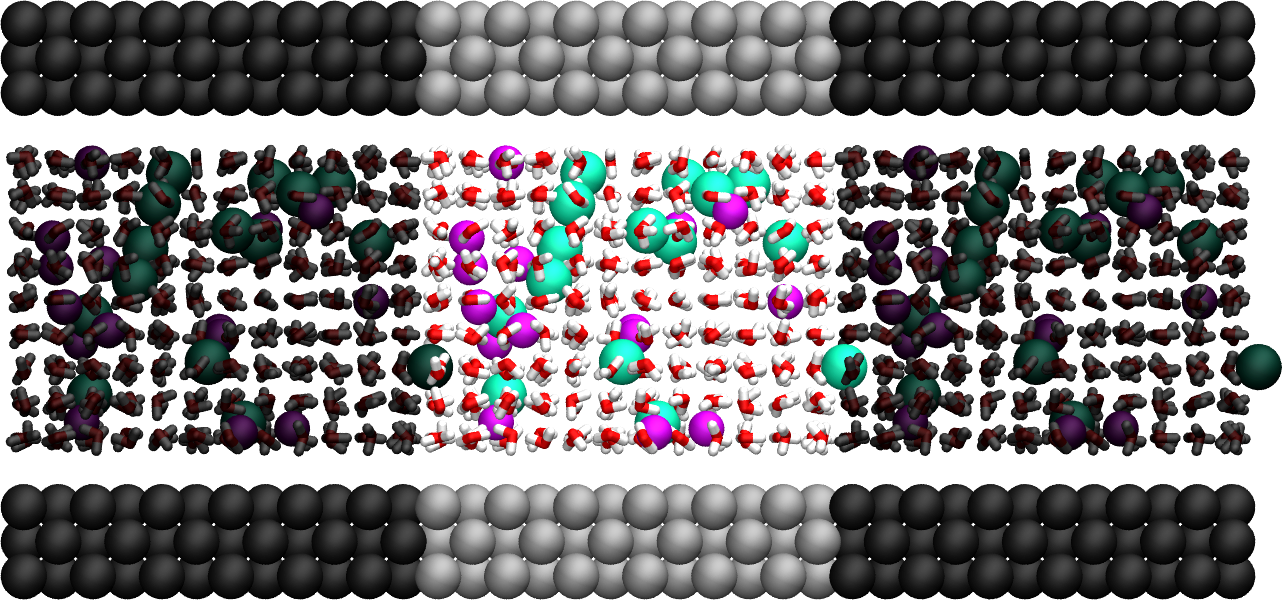
\includegraphics[width=\linewidth]{NANOSHEAR-system}
\caption{Side view of the system.  Periodic images are represented in darker colors.
Water molecules are in red and white, $\text{Na}^+$ ions in purple, $\text{Cl}^-$
ions in lime, and wall atoms in gray.  Note the absence of atomic defect at the
cell boundaries.}
\label{fig:NANOSHEAR-system}
\end{figure}

\paragraph{Energy minimization}

Let us move the atoms and place them in more energetically favorable positions
before starting the actual molecular dynamics simulation.
% SG: removed the nve/limit part for compatibility with shake
% Although we refer to this step as
% \emph{energy minimization}, it is not a conventional minimization
% like that performed in the first tutorial; \hyperref[lennard-jones-label]{Lennard-Jones fluid}.
% Instead, we will conduct a molecular dynamics simulation, employing certain techniques
% to prevent the system from exploding due to overlapping atoms.

Open the \flecmd{equilibrate.lmp} file that was downloaded alongside
\flecmd{create.lmp} during the tutorial setup.  It contains the following lines:
\begin{lstlisting}
boundary p p f
units real
atom_style full
bond_style harmonic
angle_style harmonic
pair_style lj/cut/tip4p/long O H O-H H-O-H 0.1546 12.0
kspace_style pppm/tip4p 1.0e-5
kspace_modify slab 3.0

read_data create.data

include parameters.inc
include groups.inc
\end{lstlisting}
The only difference from the previous input is that, instead of creating a new
box and new atoms, we open the previously created \flecmd{create.data} file.

Now, let us use the SHAKE algorithm to maintain the shape of the
water molecules~\cite{ryckaert1977numerical, andersen1983rattle}.
\begin{lstlisting}
fix myshk H2O shake 1.0e-5 200 0 b O-H a H-O-H kbond 2000
\end{lstlisting}
Here the SHAKE algorithm applies to the \lmpcmd{O-H} bond and the \lmpcmd{H-O-H} angle
of the water molecules.  The \lmpcmd{kbond} keyword specifies the force constant that will be
used to apply a restraint force when used during minimization.  This last keyword is important
here, because the spring constants of the rigid water molecules were set
to 0 (see the \flecmd{parameter.inc} file).
% Similar to the \lmpcmd{fix nve} command, the \lmpcmd{fix nve/limit} command performs constant
% NVE integration to update the positions and velocities of the atoms at each
% timestep.  The difference is that \lmpcmd{fix nve/limit} also limits the maximum
% distance atoms can travel during each timestep, with a chosen maximum distance
% of $0.1~\text{\AA{}}$.  Since the \lmpcmd{fix nve/limit} is applied to the
% group \lmpcmd{fluid}, only the water molecules and ions will move.
% The \lmpcmd{fix temp/berendsen} command rescales the velocities of the atoms
% to ensure the system reaches the desired temperature of $1~\text{K}$.

Let us also create images of the system and control
the printing of thermodynamic outputs by adding the following lines
to \flecmd{equilibrate.lmp}:
\begin{lstlisting}
  dump mydmp all image 1 myimage-*.ppm type type &
  shiny 0.1 box no 0.01 view 90 0 zoom 1.8
dump_modify mydmp backcolor white &
  acolor O red adiam O 2 &
  acolor H white adiam H 1 &
  acolor Na+ blue adiam Na+ 2.5 &
  acolor Cl- cyan adiam Cl- 3 &
  acolor WALL gray adiam WALL 3

thermo 1
thermo_style custom step temp etotal press
\end{lstlisting}
% The \lmpcmd{thermo\_modify} ensures that the fluid temperature \lmpcmd{Tfluid}
% is printed, and not the temperature of the entire system (which is less relevant
% with frozen walls).

Let us perform an energy minization by adding the following lines to \flecmd{equilibrate.lmp}:
\begin{lstlisting}
minimize 1.0e-6 1.0e-6 1000 1000
reset_timestep 0
\end{lstlisting}
When running the \flecmd{equilibrate.lmp} file with LAMMPS, you should observe that the
total energy of the system is initially very high but rapidly decreases.  From the generated
images of the system, you will notice that the atoms and molecules are moving to adopt more favorable positions.

% To better equilibrate the system, we will perform two additional steps
% with a larger timestep and a higher imposed temperature.  Add the following lines
% to \flecmd{minimize.lmp}:
% \begin{lstlisting}
% fix myber fluid temp/berendsen 300 300 100
% timestep 1.0

% run 4000

% unfix mynve
% fix mynve fluid nve

% run 4000

% write_data minimize.data nocoeff
% \end{lstlisting}
% For the last step, since the system is reaching a more
% equilibrated step, it is no longer necessary to use the \lmpcmd{nve/limit} command.
% Instead, we use the classic \lmpcmd{fix nve} command.

% When running the \flecmd{minimize.lmp} file with LAMMPS, you should observe that the
% the temperature reaches the desired value of $300\,\text{K}$, and that the total
% energy reaches a plateau (Fig.~\ref{fig:NANOSHEAR-minimization}).  The generated file
% \flecmd{minimize.data} contains the final state of the system.

% \begin{figure}
% \centering
% 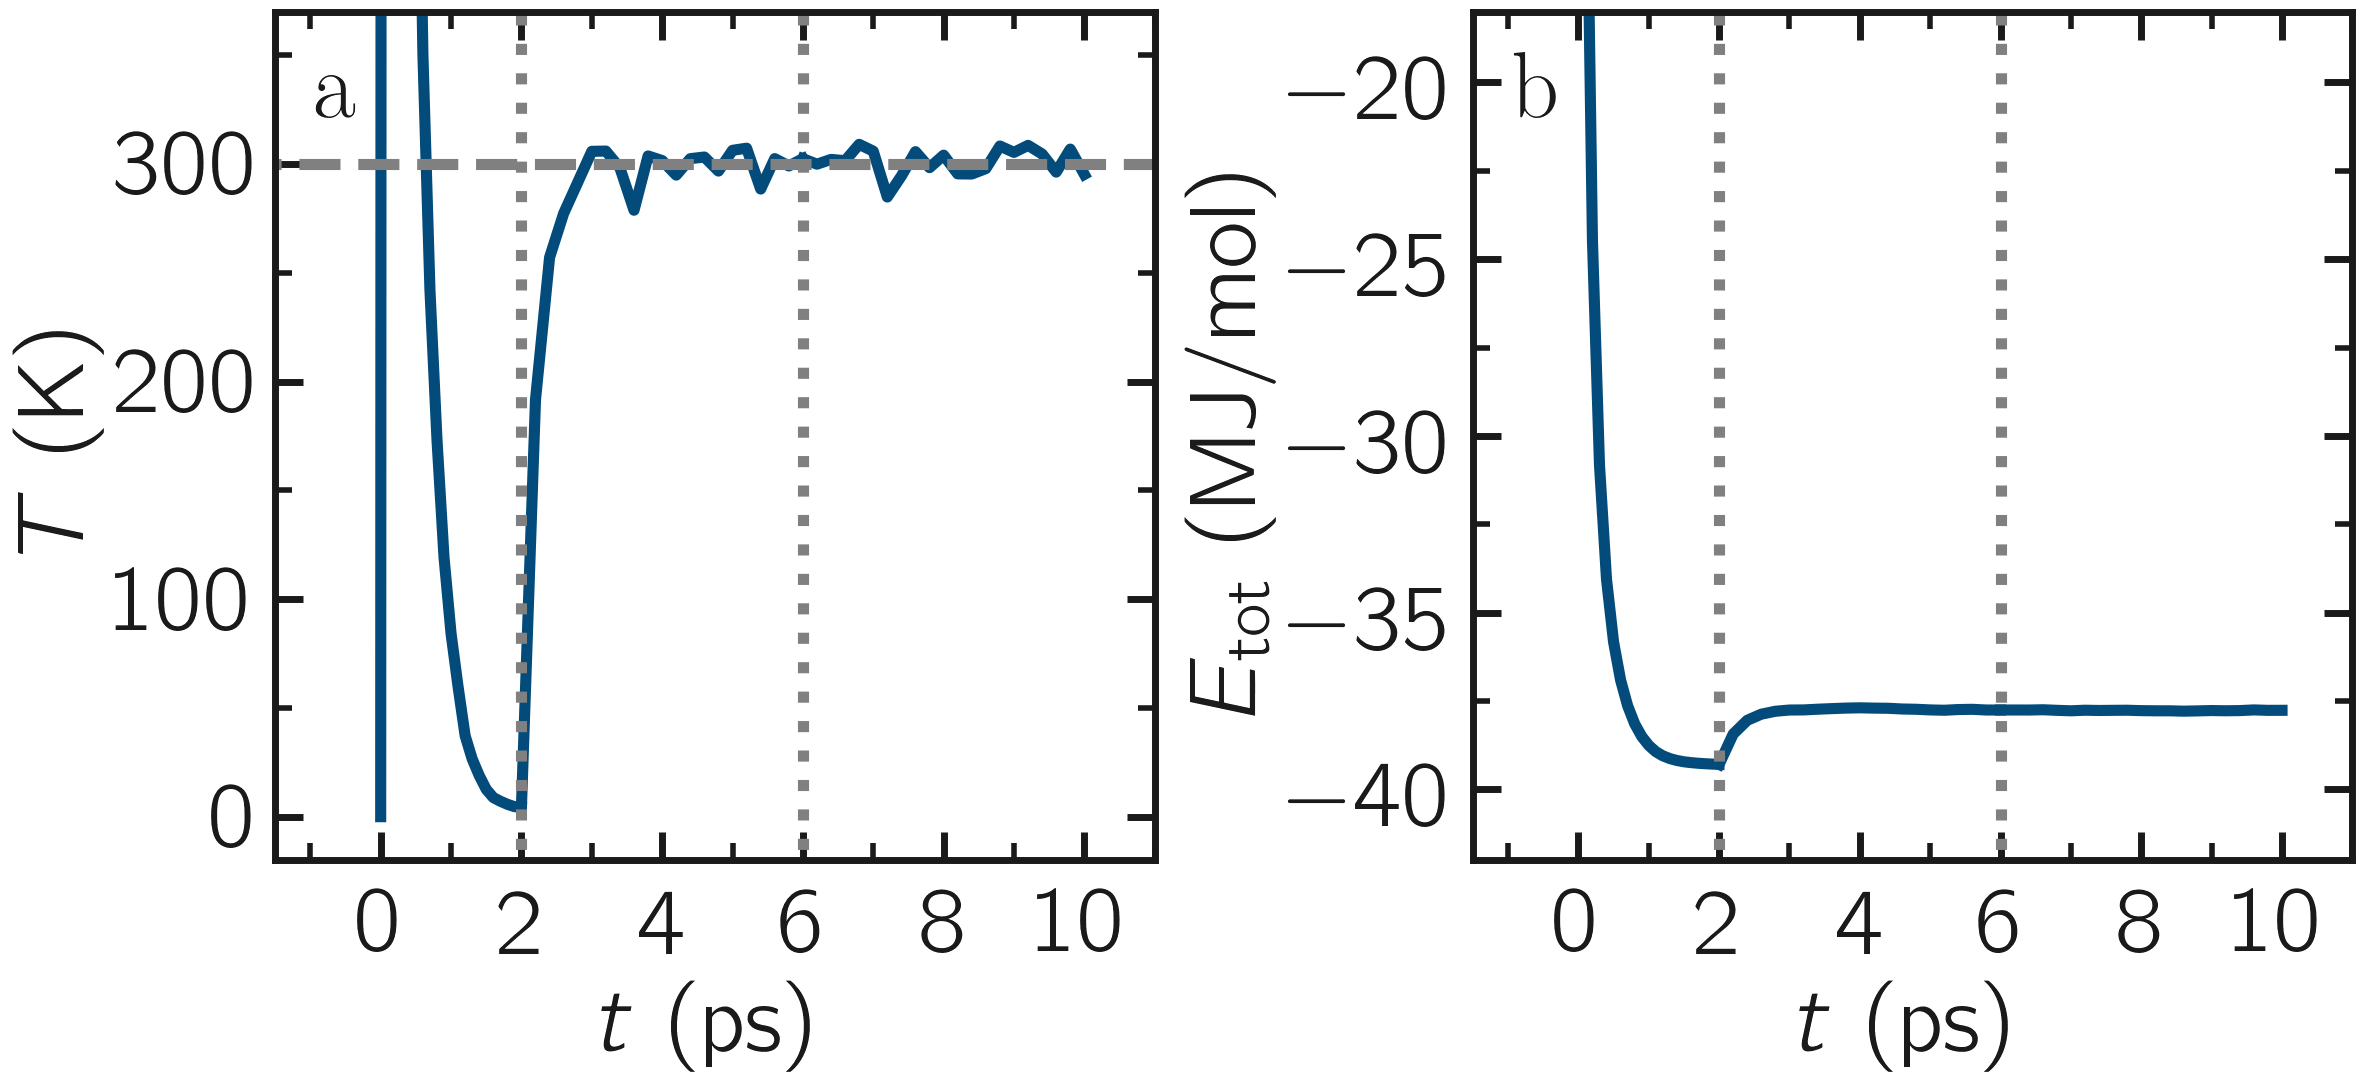
\includegraphics[width=\linewidth]{NANOSHEAR-minimization}
% \caption{a) Temperature of the fluid as a function of time $t$ during the
% minimization step of \hyperref[sheared-confined-label]{Tutorial 4}.
% The horizontal dashed line is the target temperature, $T = 300$\,K, and the
% vertical dotted lines are the transitions between the different steps
% of the minimization.  b) Total
% energy $E_\text{tot}$ of the system as a function of the time $t$.}
% \label{fig:NANOSHEAR-minimization}
% \end{figure}

\paragraph{System equilibration}

Let us equilibrate further the entire system by letting both fluid and piston
relax at ambient temperature.  Here, the commands are written within the same
\flecmd{equilibrate.lmp} file, right after the \lmpcmd{reset\_timestep} command.

Let us update the positions of all the atoms and use a Nosé-Hoover
thermostat.  Add the following lines to \flecmd{equilibrate.lmp}:
\begin{lstlisting}
fix mynvt all nvt temp 300 300 100
fix myshk H2O shake 1.0e-5 200 0 b O-H a H-O-H
fix myrct all recenter NULL NULL 0
timestep 1.0
\end{lstlisting}
As mentioned previously, the \lmpcmd{fix recenter} does not influence the dynamics,
but will keep the system in the center of the box, which makes the
visualization easier.  Then, add the following lines into \flecmd{equilibrate.lmp}
for the trajectory visualization:
\begin{lstlisting}
undump mydmp
dump mydmp all image 250 myimage-*.ppm type type &
  shiny 0.1 box no 0.01 view 90 0 zoom 1.8
dump_modify mydmp backcolor white &
  acolor O red adiam O 2 &
  acolor H white adiam H 1 &
  acolor Na+ blue adiam Na+ 2.5 &
  acolor Cl- cyan adiam Cl- 3 &
  acolor WALL gray adiam WALL 3
\end{lstlisting}
The \lmpcmd{undump} command is used to cancel the previous \lmpcmd{dump} command.
Then, a new \lmpcmd{dump} command with a larger dumping period is used.

To monitor the system equilibration, let us print the distance between
the two walls.  Add the following lines to \flecmd{equilibrate.lmp}:
\begin{lstlisting}
variable walltopz equal xcm(walltop,z)
variable wallbotz equal xcm(wallbot,z)
variable deltaz equal v_walltopz-v_wallbotz

thermo 250
thermo_style custom step temp etotal press v_deltaz
\end{lstlisting}
The first two variables extract the centers of mass of the two walls.  The
\lmpcmd{deltaz} variable is then used to calculate the difference between the two
variables \lmpcmd{walltopz} and \lmpcmd{wallbotz}, i.e.~the distance between the
two centers of mass of the walls.

Finally, let us run the simulation for 30~ps by adding a \lmpcmd{run} command
to \flecmd{equilibrate.lmp}:
\begin{lstlisting}
run 30000

write_data equilibrate.data nocoeff
\end{lstlisting}
Run the \flecmd{equilibrate.lmp} file using LAMMPS.  Both the pressure and the distance
between the two walls show oscillations at the start of the simulation
but eventually stabilize at their equilibrium values toward
the end of the simulation (Fig.~\ref{fig:NANOSHEAR-equilibration}).

\begin{note}
Note that it is generally recommended to run a longer equilibration.  In this case,
the slowest process in the system is likely ionic diffusion.
Therefore, the equilibration period should, in principle, exceed the time required
for the ions to diffuse across the size of the pore, i.e.~$H_\text{pore}^2/D_\text{ions}$.
Using $H_\text{pore} \approx 1.2~\text{nm}$ as the final pore size
and $D_\text{ions} \approx 1.5 \cdot 10^{-9}~\text{m}^2/\text{s}$
as the typical diffusion coefficient for sodium chloride in water at room
temperature~\cite{mills1955remeasurement}, one finds that the equilibration
should be on the order of one nanosecond.
\end{note}

\begin{figure}
\centering
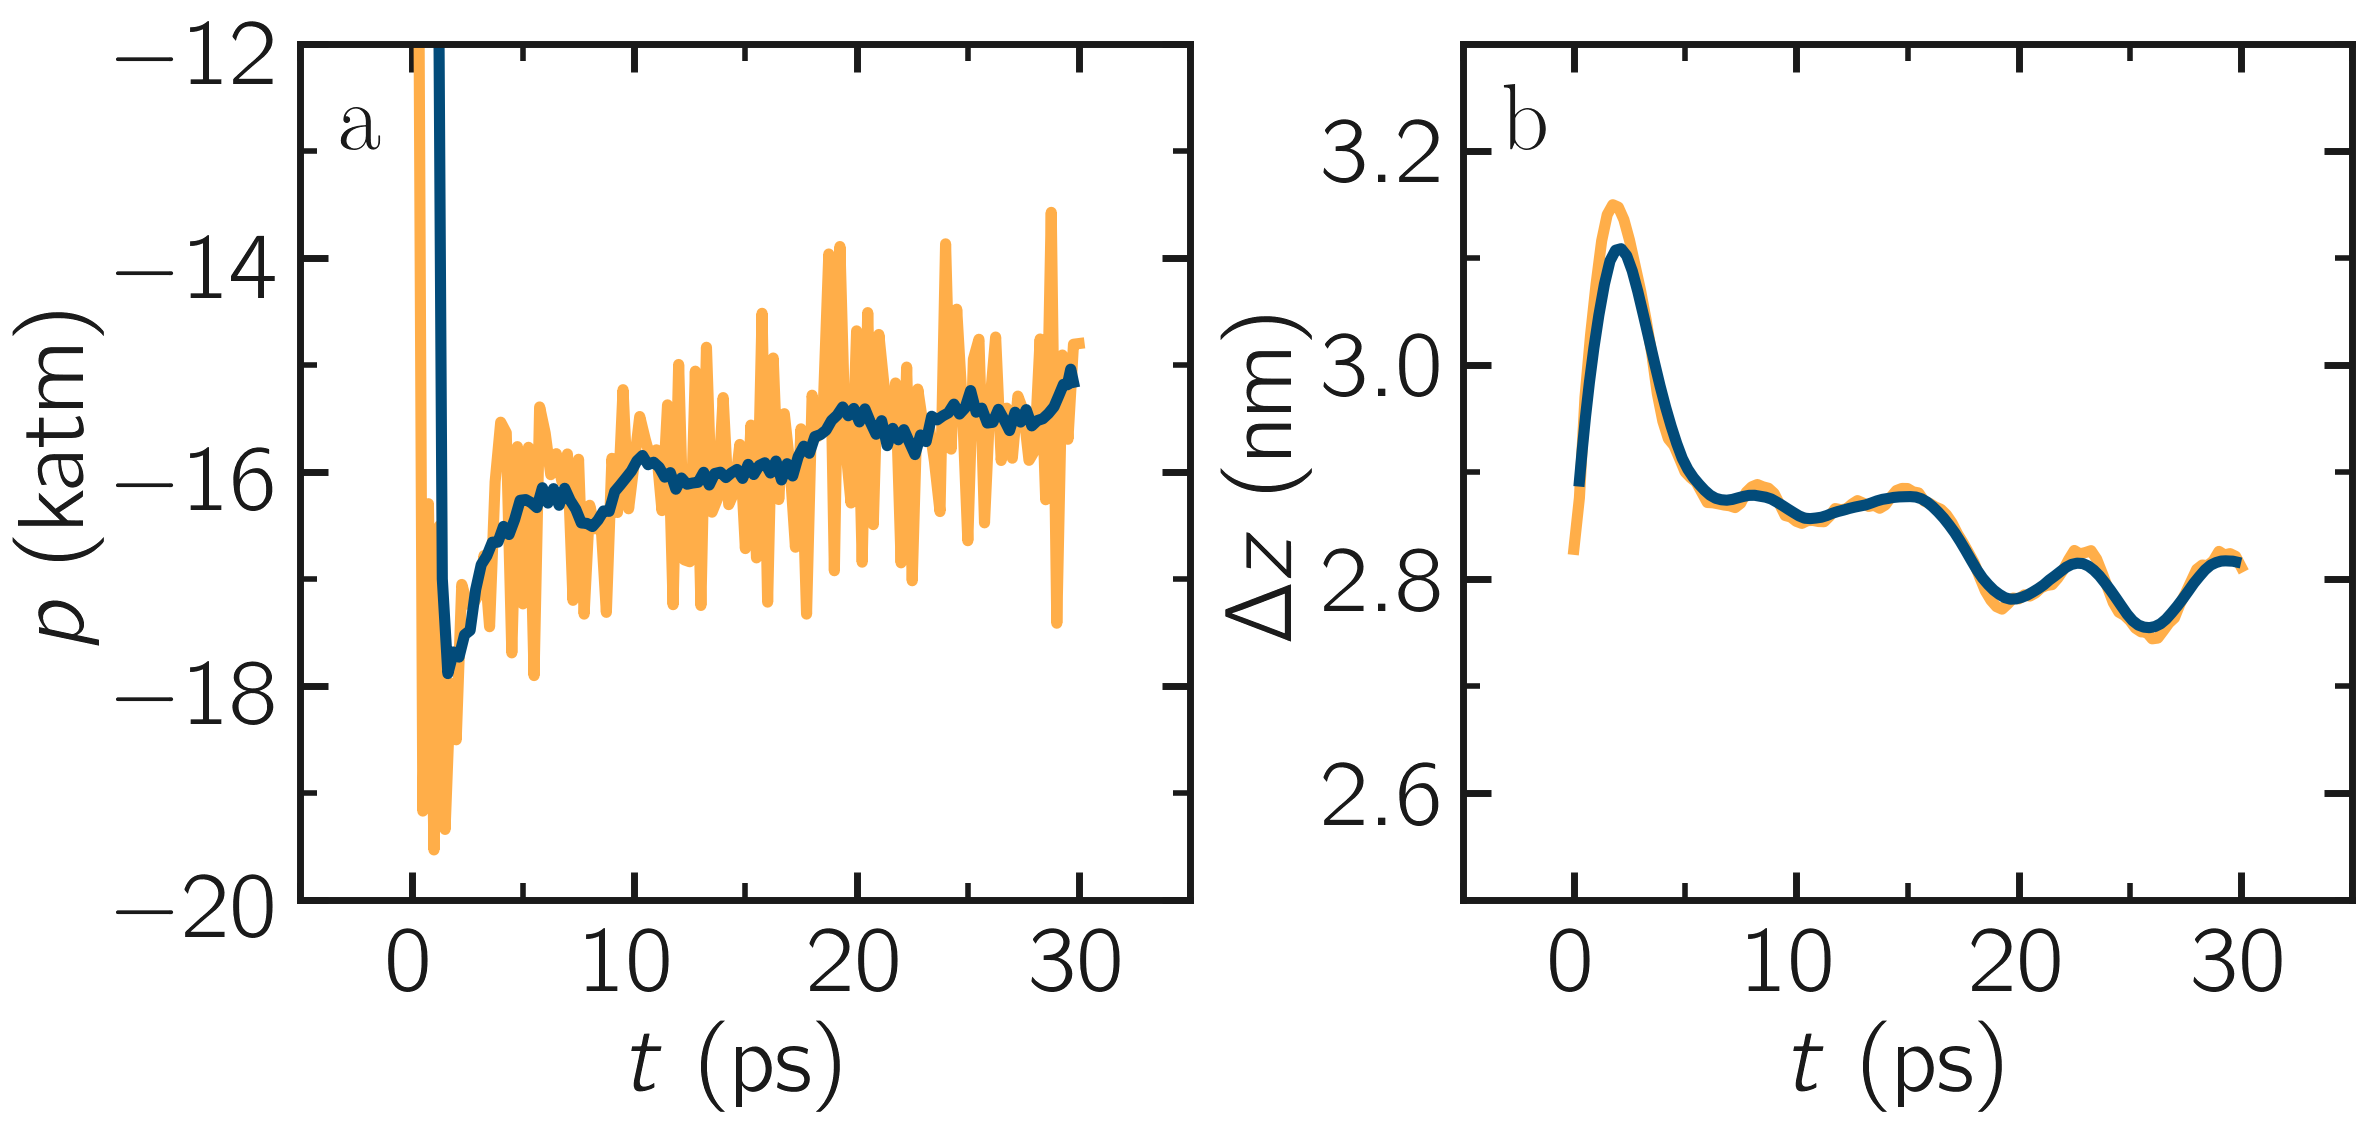
\includegraphics[width=\linewidth]{NANOSHEAR-equilibration}
\caption{a)~Pressure $p$ of the nanosheared electrolyte system
simulated in \hyperref[sheared-confined-label]{Tutorial 4} as a function of the
time $t$.  b)~Distance between the walls $\Delta z$ as a function of time $t$.}
\label{fig:NANOSHEAR-equilibration}
\end{figure}

\subsubsection{Imposed shearing}

From the equilibrated configuration, let us impose a lateral motion on the two
walls and shear the electrolyte.  Open the last input file named \flecmd{shearing.lmp}.
It starts with the following lines:
\begin{lstlisting}
boundary p p f
units real
atom_style full
bond_style harmonic
angle_style harmonic
pair_style lj/cut/tip4p/long O H O-H H-O-H 0.1546 12.0
kspace_style pppm/tip4p 1.0e-5
kspace_modify slab 3.0

read_data equilibrate.data

include parameters.inc
include groups.inc
\end{lstlisting}

To address the dynamics of the system, add the following lines to
\flecmd{shearing.lmp}:
\begin{lstlisting}
compute Tfluid fluid temp/partial 0 1 1
fix mynvt1 fluid nvt temp 300 300 100
fix_modify mynvt1 temp Tfluid

compute Twall wall temp/partial 0 1 1
fix mynvt2 wall nvt temp 300 300 100
fix_modify mynvt2 temp Twall

fix myshk H2O shake 1.0e-5 200 0 b O-H a H-O-H
fix myrct all recenter NULL NULL 0
timestep 1.0
\end{lstlisting}
One key difference with the previous input is that, here, two thermostats are used,
one for the fluid (\lmpcmd{mynvt1}) and one for the solid (\lmpcmd{mynvt2}).
The combination of \lmpcmd{fix\_modify} with \lmpcmd{compute temp} ensures
that the correct temperature values are used by the thermostats.  Using
\lmpcmd{compute} commands for the temperature with \lmpcmd{temp/partial 0 1 1} is
intended to exclude the $x$ coordinate from the thermalization, which is important since a
large velocity will be imposed along the $x$ direction.

Then, let us impose the velocity of the two walls by adding the following
commands to \flecmd{shearing.lmp}:
\begin{lstlisting}
fix mysf1 walltop setforce 0 NULL NULL
fix mysf2 wallbot setforce 0 NULL NULL
velocity wallbot set -2e-4 NULL NULL
velocity walltop set 2e-4 NULL NULL
\end{lstlisting}
The \lmpcmd{setforce} commands cancel the forces on \lmpcmd{walltop} and
\lmpcmd{wallbot}.  As a result, the atoms in these two groups will not
experience any forces from the rest of the system.  Consequently, in the absence of
external forces, these atoms will conserve the initial velocities imposed by the
two \lmpcmd{velocity} commands.

Finally, let us generate images of the systems and print the values of the
forces exerted by the fluid on the walls, as given by \lmpcmd{f\_mysf1[1]}
and \lmpcmd{f\_mysf2[1]}.  Add these lines to \flecmd{shearing.lmp}:
\begin{lstlisting}
dump mydmp all image 250 myimage-*.ppm type type &
  shiny 0.1 box no 0.01 view 90 0 zoom 1.8
dump_modify mydmp backcolor white &
  acolor O red adiam O 2 &
  acolor H white adiam H 1 &
  acolor Na+ blue adiam Na+ 2.5 &
  acolor Cl- cyan adiam Cl- 3 &
  acolor WALL gray adiam WALL 3

thermo 250
thermo_modify temp Tfluid
thermo_style custom step temp etotal f_mysf1[1] f_mysf2[1]
\end{lstlisting}
Let us also extract the density and velocity profiles using
the \lmpcmd{chunk/atom} and \lmpcmd{ave/chunk} commands.  These commands are
used to divide the system into bins and return the desired quantities, here the velocity
along $x$ (\lmpcmd{vx}) within the bins.  Add the following lines to \flecmd{shearing.lmp}:
\begin{lstlisting}
compute cc1 H2O chunk/atom bin/1d z 0.0 0.25
compute cc2 wall chunk/atom bin/1d z 0.0 0.25
compute cc3 ions chunk/atom bin/1d z 0.0 0.25

fix myac1 H2O ave/chunk 10 15000 200000 &
  cc1 density/mass vx file shearing-water.dat
fix myac2 wall ave/chunk 10 15000 200000 &
  cc2 density/mass vx file shearing-wall.dat
fix myac3 ions ave/chunk 10 15000 200000 &
  cc3 density/mass vx file shearing-ions.dat

run 200000
\end{lstlisting}
Here, a bin size of $0.25\,\text{\AA{}}$ is used for the density profiles generated
by the \lmpcmd{ave/chunk} commands, and three \flecmd{.dat} files are created for
the water, the walls, and the ions, respectively.  With values of \lmpcmd{10 15000 200000},
the velocity \lmpcmd{vx} will be evaluated every 10 steps during the final 150,000
steps of the simulations.  The result will be averaged and printed only once at the 200,000\,th step.
Run the simulation using LAMMPS.  The averaged velocity
profile for the fluid is plotted in Fig.~\ref{fig:NANOSHEAR-profiles}.
As expected for such Couette flow geometry, the fluid velocity increases
linearly along $z$, and is equal to the walls velocities at the fluid-solid
interfaces (no-slip boundary conditions).

\begin{figure}
\centering
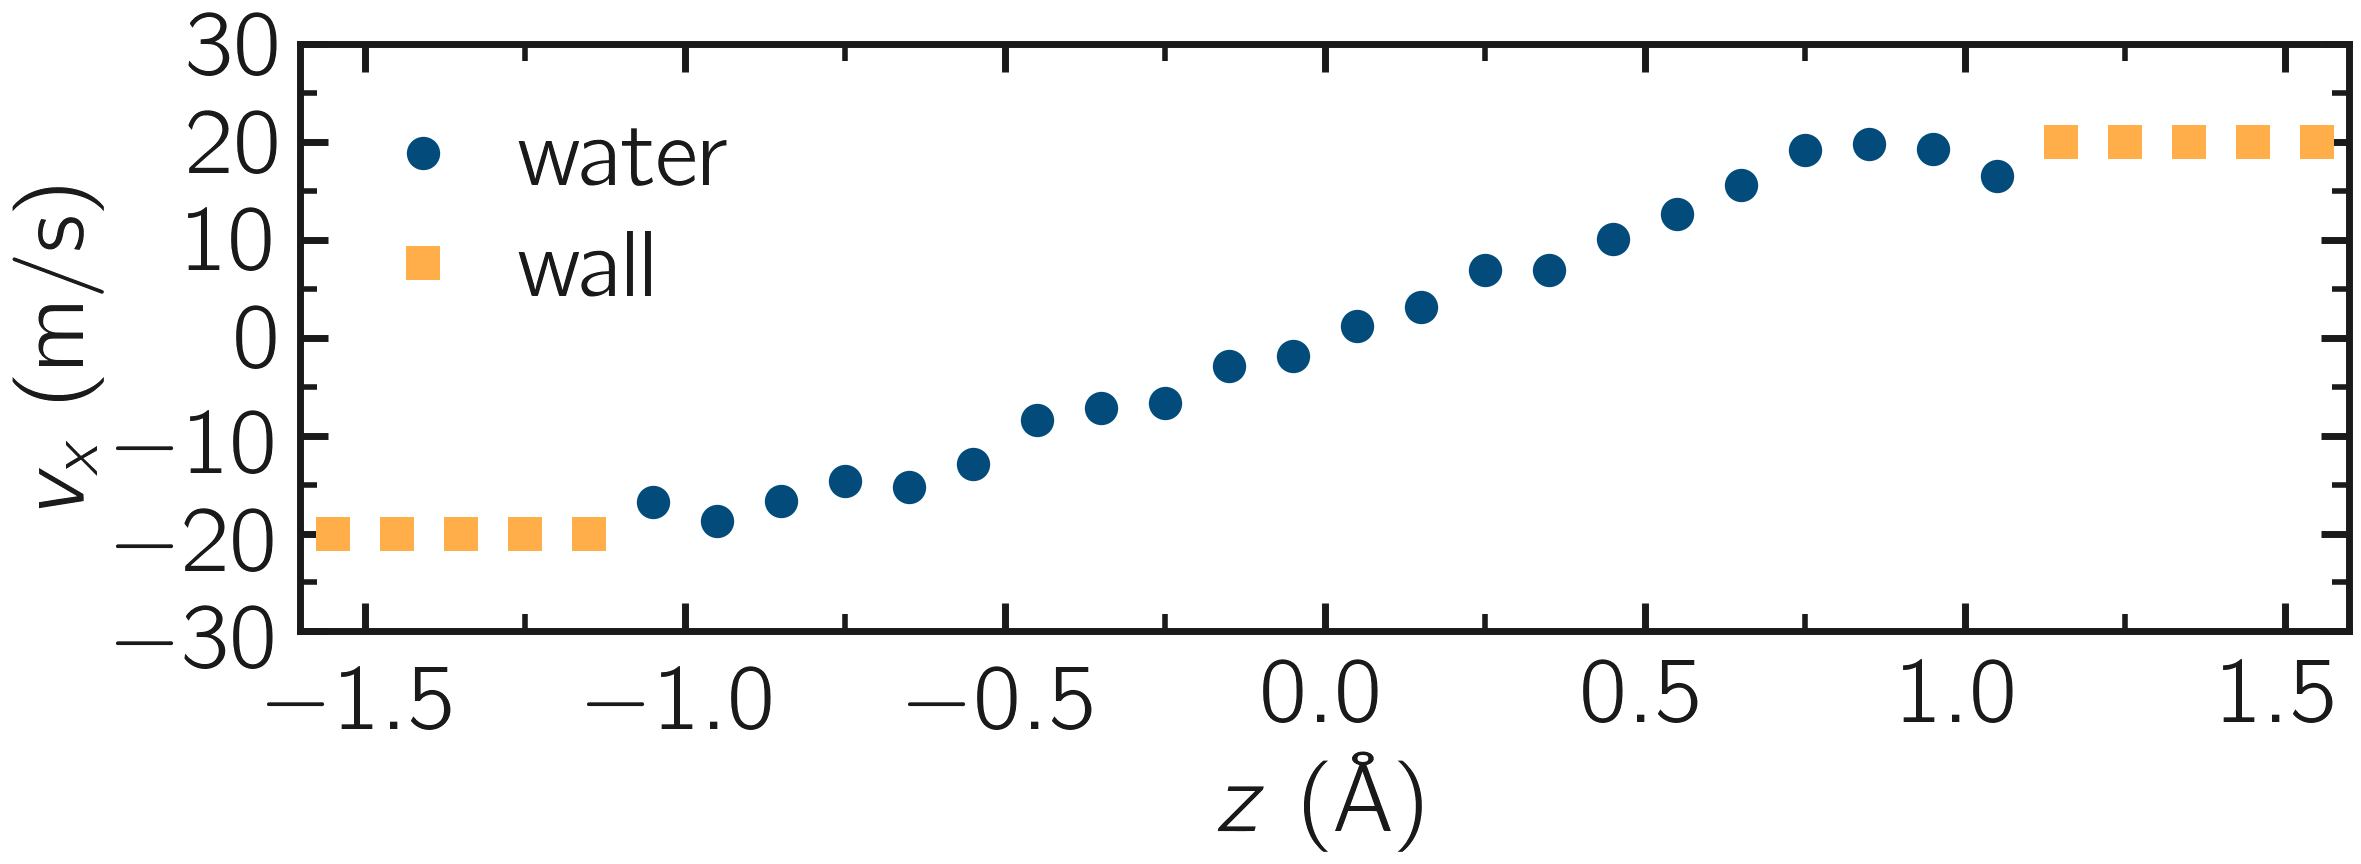
\includegraphics[width=\linewidth]{NANOSHEAR-profiles}
\caption{Velocity profiles for water (blue) and walls (orange) along the $z$-axis as
simulated in \hyperref[sheared-confined-label]{Tutorial 4}.}
% The line is a linear fit assuming
% that the pore size is $h = 1.8\,\text{nm}$.}
\label{fig:NANOSHEAR-profiles}
\end{figure}

From the force applied by the fluid on the solid, one can extract the stress
within the fluid, which enables the measurement of its viscosity $\eta$
according to
\begin{equation}
\eta = \tau / \dot{\gamma}
\label{eq:eta}
\end{equation}
where $\tau$ is the stress applied by
the fluid on the shearing wall, and $\dot{\gamma}$ the shear rate
\cite{gravelle2021violations}.  Here, the shear rate is
approximately $\dot{\gamma} = 20 \cdot 10^9\,\text{s}^{-1}$ (Fig.~\ref{fig:NANOSHEAR-profiles}),
the average force on each wall is given by \lmpcmd{f\_mysf1[1]} and \lmpcmd{f\_mysf2[1]}
and is approximately $2.7\,\mathrm{kcal/mol/\AA}$ in magnitude.  Using a surface area
for the walls of $A = 6 \cdot 10^{-18}\,\text{m}^2$, one obtains an estimate for
the shear viscosity for the confined fluid of $\eta = 3.1\,\text{mPa.s}$ using Eq.~\eqref{eq:eta}.

\begin{note}
The viscosity calculated at such a high shear rate may differ from the expected
\emph{bulk} value.  In general, it is recommended to use a lower value for the
shear rate.  Note that for lower shear rates, the ratio of noise-to-signal is
larger, and longer simulations are needed.  Another important point to consider
is that the viscosity of a fluid next to a solid surface is typically larger
than in bulk due to interaction with the walls~\cite{wolde-kidanInterplayInterfacialViscosity2021}.
Therefore, one expects the present simulation to yield a viscosity that is slightly
higher than what would be measured in the absence of walls.
\end{note}

\subsection{Tutorial 5: Reactive silicon dioxide}
\label{reactive-silicon-dioxide-label}

\begin{figure}
\centering
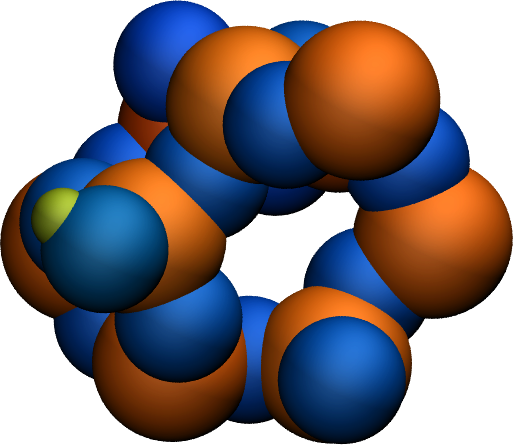
\includegraphics[width=0.55\linewidth]{SIO}
\caption{A portion of the silicon dioxide structure as simulated during
\hyperref[reactive-silicon-dioxide-label]{Tutorial 5}.  Atoms are colored
by their charges: the hydrogen atoms appear as small greenish spheres, silicon
atoms as large orange spheres, and oxygen atoms as blue spheres of intermediate
size.}
\label{fig:SIO}
\end{figure}

The objective of this tutorial is to demonstrate how the reactive force field ReaxFF
can be used to calculate the partial charges of a system undergoing deformation, as well as
the formation and breaking of chemical bonds~\cite{van2001reaxff, zou2012investigation}.
The system simulated in this tutorial is a block of silicon dioxide $\text{SiO}_2$ (Fig.~\ref{fig:SIO})
which is deformed until it ruptures.  Particular attention is given to the evolution
of atomic charges during deformation, with a focus on tracking chemical reactions
resulting from the deformation over time.

\subsubsection{Prepare and relax}

The first step is to relax the structure with ReaxFF, which which will be achieved using
molecular dynamics.  To ensure the system equilibrates properly, we will monitor certain
parameters over time, such as the system volume.  To set up this
tutorial, select \guicmd{Start Tutorial 5} from the
\guicmd{Tutorials} menu of \lammpsgui{} and follow the instructions.
The editor should display the following content corresponding to \flecmd{relax.lmp}:
\begin{lstlisting}
units real
atom_style full

read_data silica.data

\end{lstlisting}
So far, the input is very similar to what was seen in the previous tutorials.
Some basic parameters are defined (\lmpcmd{units} and \lmpcmd{atom\_style}),
and a \lmpcmd{.data} file is imported by the \lmpcmd{read\_data} command.

The initial topology given by \href{\filepath tutorial5/silica.data}{\dwlcmd{silica.data}}
is a small amorphous silica structure.  This structure was created using a force field called
Vashishta~\cite{vashishta1990interaction}.  If you open the \flecmd{silica.data}
file, you will find in the \lmpcmd{Atoms} section that all silicon atoms have a
charge of $q = 1.1\,\text{e}$, and all oxygen atoms have a charge of $q = -0.55\,\text{e}$.

\begin{note}
Assigning the same charge to all atoms of the same type is common with many
force fields, including the force fields used in the previous tutorials.  This
changes once ReaxFF is used: the charge of each atom will adjust to its local
environment.
\end{note}

Next, copy the following three crucial lines into the \flecmd{relax.lmp} file:
\begin{lstlisting}
pair_style reaxff NULL safezone 3.0 mincap 150
pair_coeff * * reaxCHOFe.inc Si O
fix myqeq all qeq/reaxff 1 0.0 10.0 1.0e-6 reaxff maxiter 400
\end{lstlisting}
In this case, the \lmpcmd{pair\_style reaxff} is used without a control file.  The
\lmpcmd{safezone} and \lmpcmd{mincap} keywords are added to prevent
allocation issues, which sometimes can trigger segmentation faults and
\lmpcmd{bondchk} errors.  The \lmpcmd{pair\_coeff} command uses the
\href{\filepath tutorial5/reaxCHOFe.inc}{\dwlcmd{reaxCHOFe.inc}}
file, which should have been downloaded during the tutorial set up.  Finally, the
\lmpcmd{fix qeq/reaxff} is used to perform charge equilibration~\cite{rappe1991charge},
which occurs at every step.  The values 0.0 and 10.0 represent the
low and the high cutoffs, respectively, and $1.0 \text{e} -6$ is the tolerance.
The \lmpcmd{maxiter} sets an upper limit to the number of attempts to
equilibrate the charge.

Next, add the following commands to the \flecmd{relax.lmp} file to track the
evolution of the charges during the simulation:
\begin{lstlisting}
group grpSi type Si
group grpO type O
variable qSi equal charge(grpSi)/count(grpSi)
variable qO equal charge(grpO)/count(grpO)
variable vq atom q
\end{lstlisting}
To print the averaged charges \lmpcmd{qSi} and \lmpcmd{qO} using the
\lmpcmd{thermo\_style} command, and create images of the system.  Add the
following lines to \flecmd{relax.lmp}:
\begin{lstlisting}
thermo 100
thermo_style custom step temp etotal press vol v_qSi v_qO
dump viz all image 100 myimage-*.ppm q &
  type shiny 0.1 box no 0.01 view 180 90 zoom 2.3 size 1200 500
dump_modify viz adiam Si 2.6 adiam O 2.3 backcolor white &
  amap -1 2 ca 0.0 3 min royalblue 0 green max orangered
\end{lstlisting}
Here, the atoms are colored by their charges \lmpcmd{q}, ranging from royal blue
(when $q=-1\,\text{e}$) to orange-red (when $q=2\,\text{e}$).

You can generate histograms of the charges for each atom type using
\lmpcmd{fix ave/histo} commands:
\begin{lstlisting}
fix myhis1 grpSi ave/histo 10 500 5000 -1.5 2.5 1000 v_vq &
  file relax-Si.histo mode vector
fix myhis2 grpO ave/histo 10 500 5000 -1.5 2.5 1000 v_vq &
  file relax-O.histo mode vector
\end{lstlisting}
We can also use the \lmpcmd{fix reaxff/species} to evaluate what species are
present within the simulation.  It will be useful later when the system is deformed,
and bonds are broken:
\begin{lstlisting}
fix myspec all reaxff/species 5 1 5 relax.species element Si O
\end{lstlisting}
Here, the information will be printed every 5 steps in a file called \flecmd{relax.species}.
Let us perform a very short run using the anisotropic NPT command and relax the
density of the system.
\begin{lstlisting}
velocity all create 300.0 32028
fix mynpt all npt temp 300.0 300.0 100 aniso 1.0 1.0 1000
timestep 0.5

run 5000

write_data relax.data
\end{lstlisting}
Run the \flecmd{relax.lmp} file using LAMMPS.  As seen from \flecmd{relax.species},
only one species is detected, called \lmpcmd{O384Si192}, representing the entire system.

As the simulation progresses, the charge of every atom fluctuates
because it is adjusting to the local environment of the atom (Fig.~\ref{fig:SIO-charge}\,a).
It is also observed that the averaged charges for silicon and oxygen
atoms fluctuate significantly at the beginning of the simulation, corresponding
to a rapid change in the system volume, which causes interatomic distances to
shift quickly (Fig.~\ref{fig:SIO-charge}\,b).  The atoms with the
most extreme charges are located at structural defects,
such as dangling oxygen groups (Fig.~\ref{fig:SIO-slice}).
Finally, the charge distribution $P(q)$ can be plotted using the charge values
from the \flecmd{.histo} files (Fig.~\ref{fig:SIO-distribution}\,a).

\begin{figure}
\centering
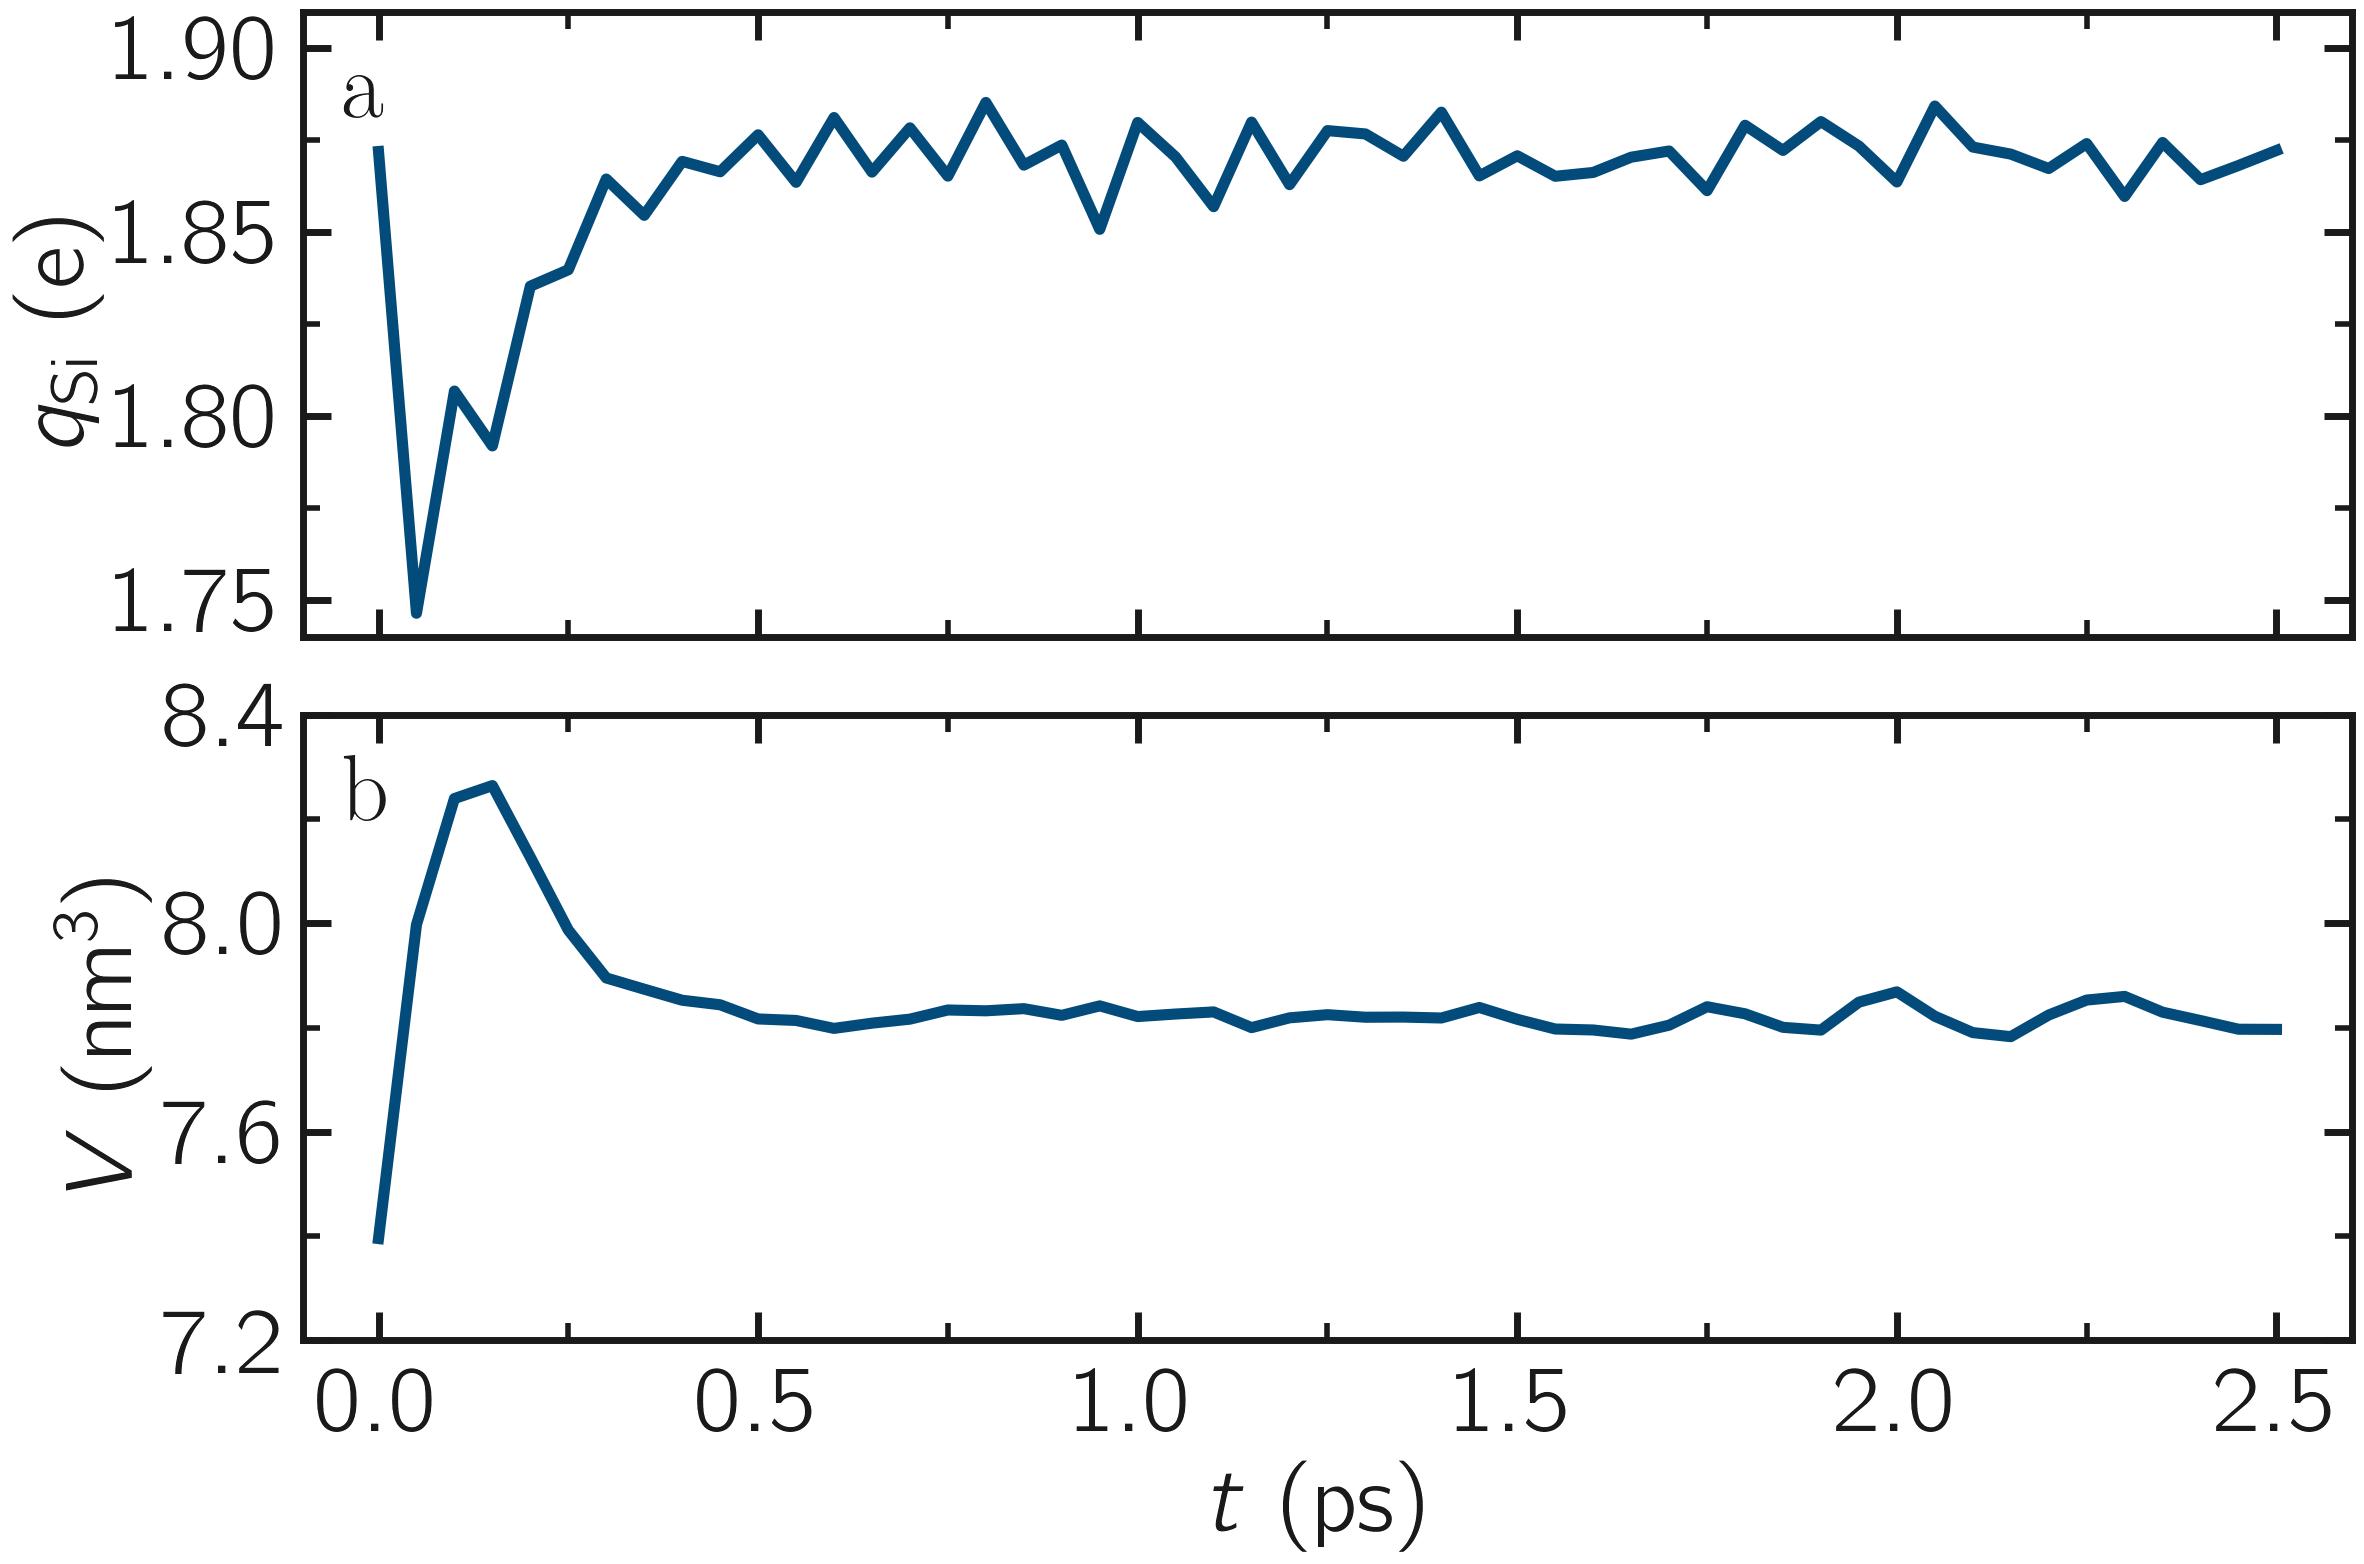
\includegraphics[width=\linewidth]{SIO-charge}
\caption{a) Average charge per atom of the silicon $q_\text{Si}$ atoms as
a function of time $t$ during equilibration of the $\text{SiO}_2$ system
from \hyperref[reactive-silicon-dioxide-label]{Tutorial 5}.  b) Volume of the
system $V$ as a function of time $t$.}
\label{fig:SIO-charge}
\end{figure}

\begin{figure}
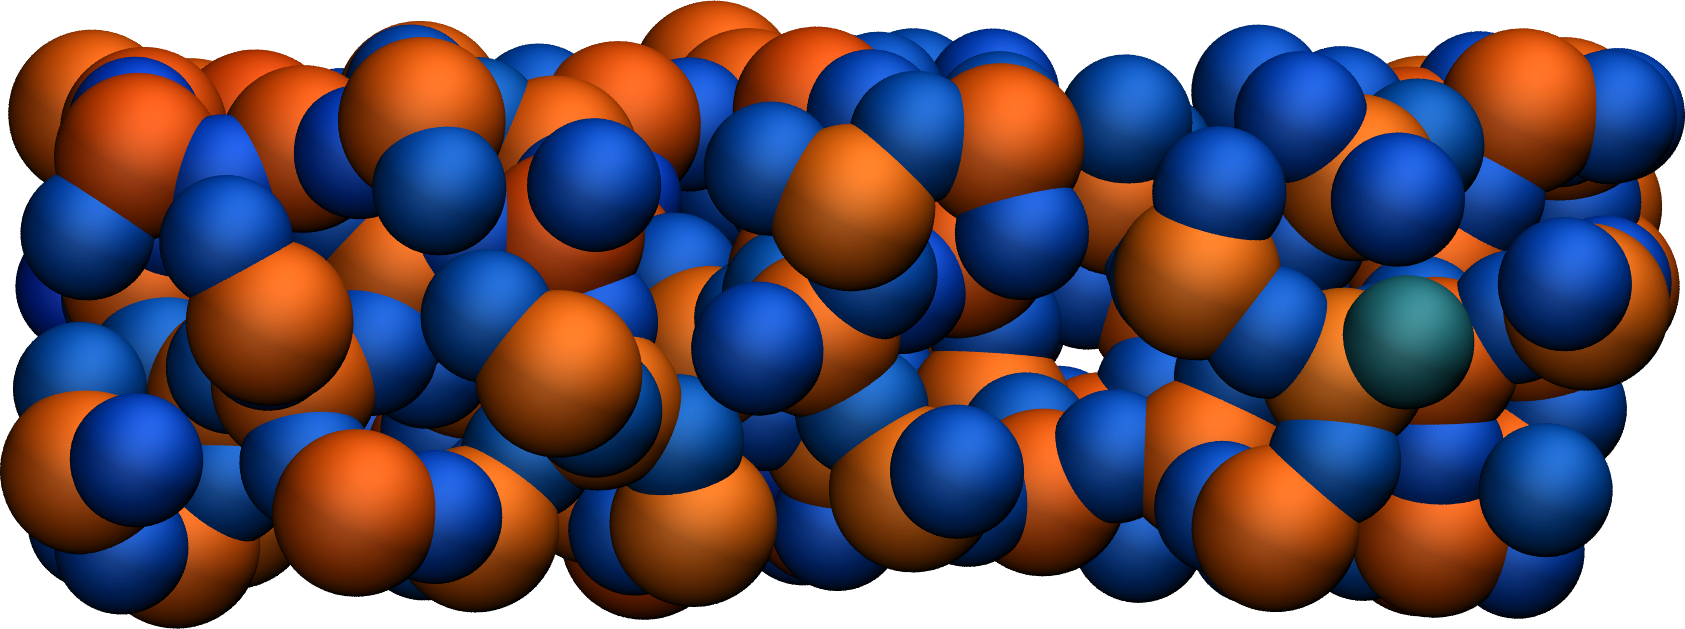
\includegraphics[width=\linewidth]{SIO-slice}
\caption{A slice of the amorphous silica simulated during
\hyperref[reactive-silicon-dioxide-label]{Tutorial 5}, where atoms are colored by their charges.
Dangling oxygen groups appear in greenish, bulk Si atoms with a charge of about
$1.8~\text{e}$  appear in red/orange, and bulk O atoms with a charge of about
$-0.9~\text{e}$ appear in blue.}
\label{fig:SIO-slice}
\end{figure}

\begin{figure}
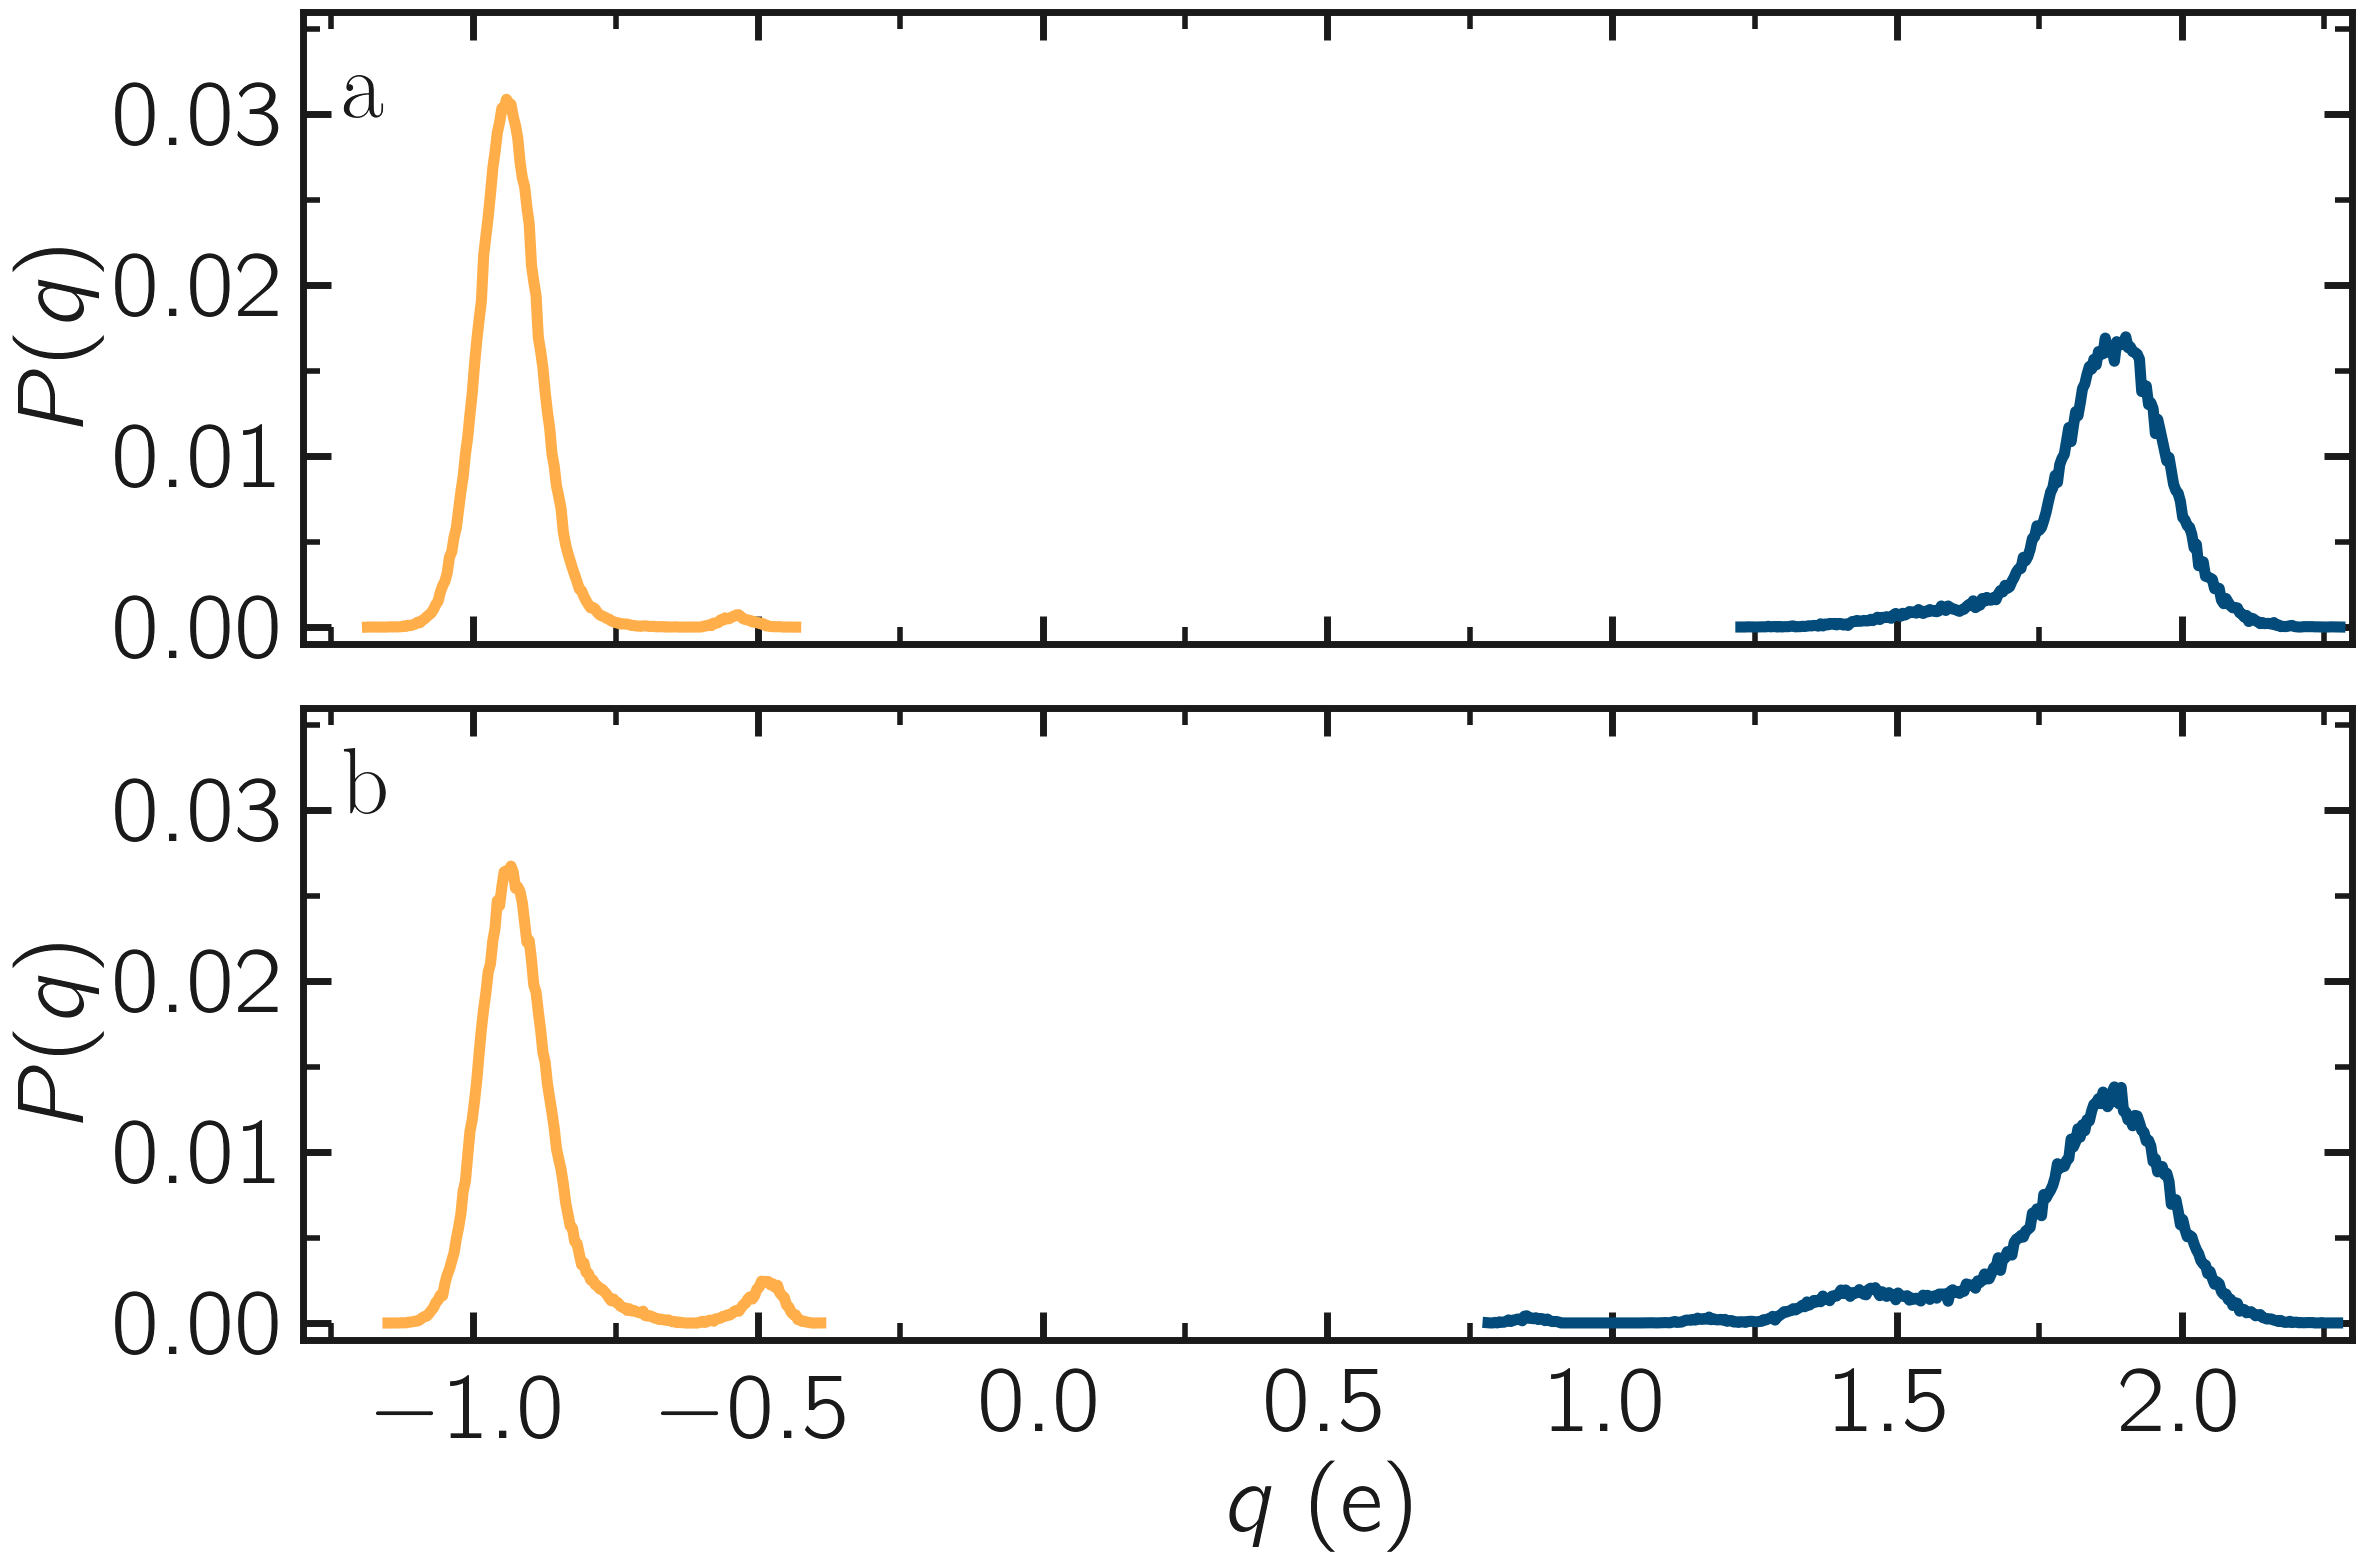
\includegraphics[width=\linewidth]{SIO-distribution}
\caption{a) Probability distributions of charge of silicon (positive, blue) and oxygen
(negative, orange) atoms during the equilibration of the $\text{SiO}_2$ system
from \hyperref[reactive-silicon-dioxide-label]{Tutorial 5}.  b) Same probability distributions
after the deformation.}
\label{fig:SIO-distribution}
\end{figure}

\subsubsection{Deform the structure}

Let us apply a deformation to the structure to force some $\text{Si}-\text{O}$
bonds to break (and eventually re-assemble).  Open the \flecmd{deform.lmp}
file, which must contain the following lines:
\begin{lstlisting}
units real
atom_style full

read_data relax.data

pair_style reaxff NULL safezone 3.0 mincap 150
pair_coeff * * reaxCHOFe.inc Si O
fix myqeq all qeq/reaxff 1 0.0 10.0 1.0e-6 reaxff maxiter 400

group grpSi type Si
group grpO type O
variable qSi equal charge(grpSi)/count(grpSi)
variable qO equal charge(grpO)/count(grpO)
variable vq atom q

thermo 200
thermo_style custom step temp etotal press vol v_qSi v_qO
dump viz all image 100 myimage-*.ppm q &
  type shiny 0.1 box no 0.01 view 180 90 zoom 2.3 size 1200 500
dump_modify viz adiam Si 2.6 adiam O 2.3 backcolor white &
  amap -1 2 ca 0.0 3 min royalblue 0 green max orangered

fix myhis1 grpSi ave/histo 10 500 5000 -1.5 2.5 1000 v_vq &
  file deform-Si.histo mode vector
fix myhis2 grpO ave/histo 10 500 5000 -1.5 2.5 1000 v_vq &
  file deform-O.histo mode vector
fix myspec all reaxff/species 5 1 5 deform.species element Si O
\end{lstlisting}
The only difference with the previous \flecmd{relax.lmp} file is the path to
the \flecmd{relax.data} file.

Next, let us use \lmpcmd{fix nvt} instead of \lmpcmd{fix npt} to apply a
Nosé-Hoover thermostat without a barostat:
\begin{lstlisting}
fix mynvt all nvt temp 300.0 300.0 100
timestep 0.5
\end{lstlisting}
Here, no barostat is used because the change in the box volume will be imposed
by the \lmpcmd{fix deform}.

\begin{figure}
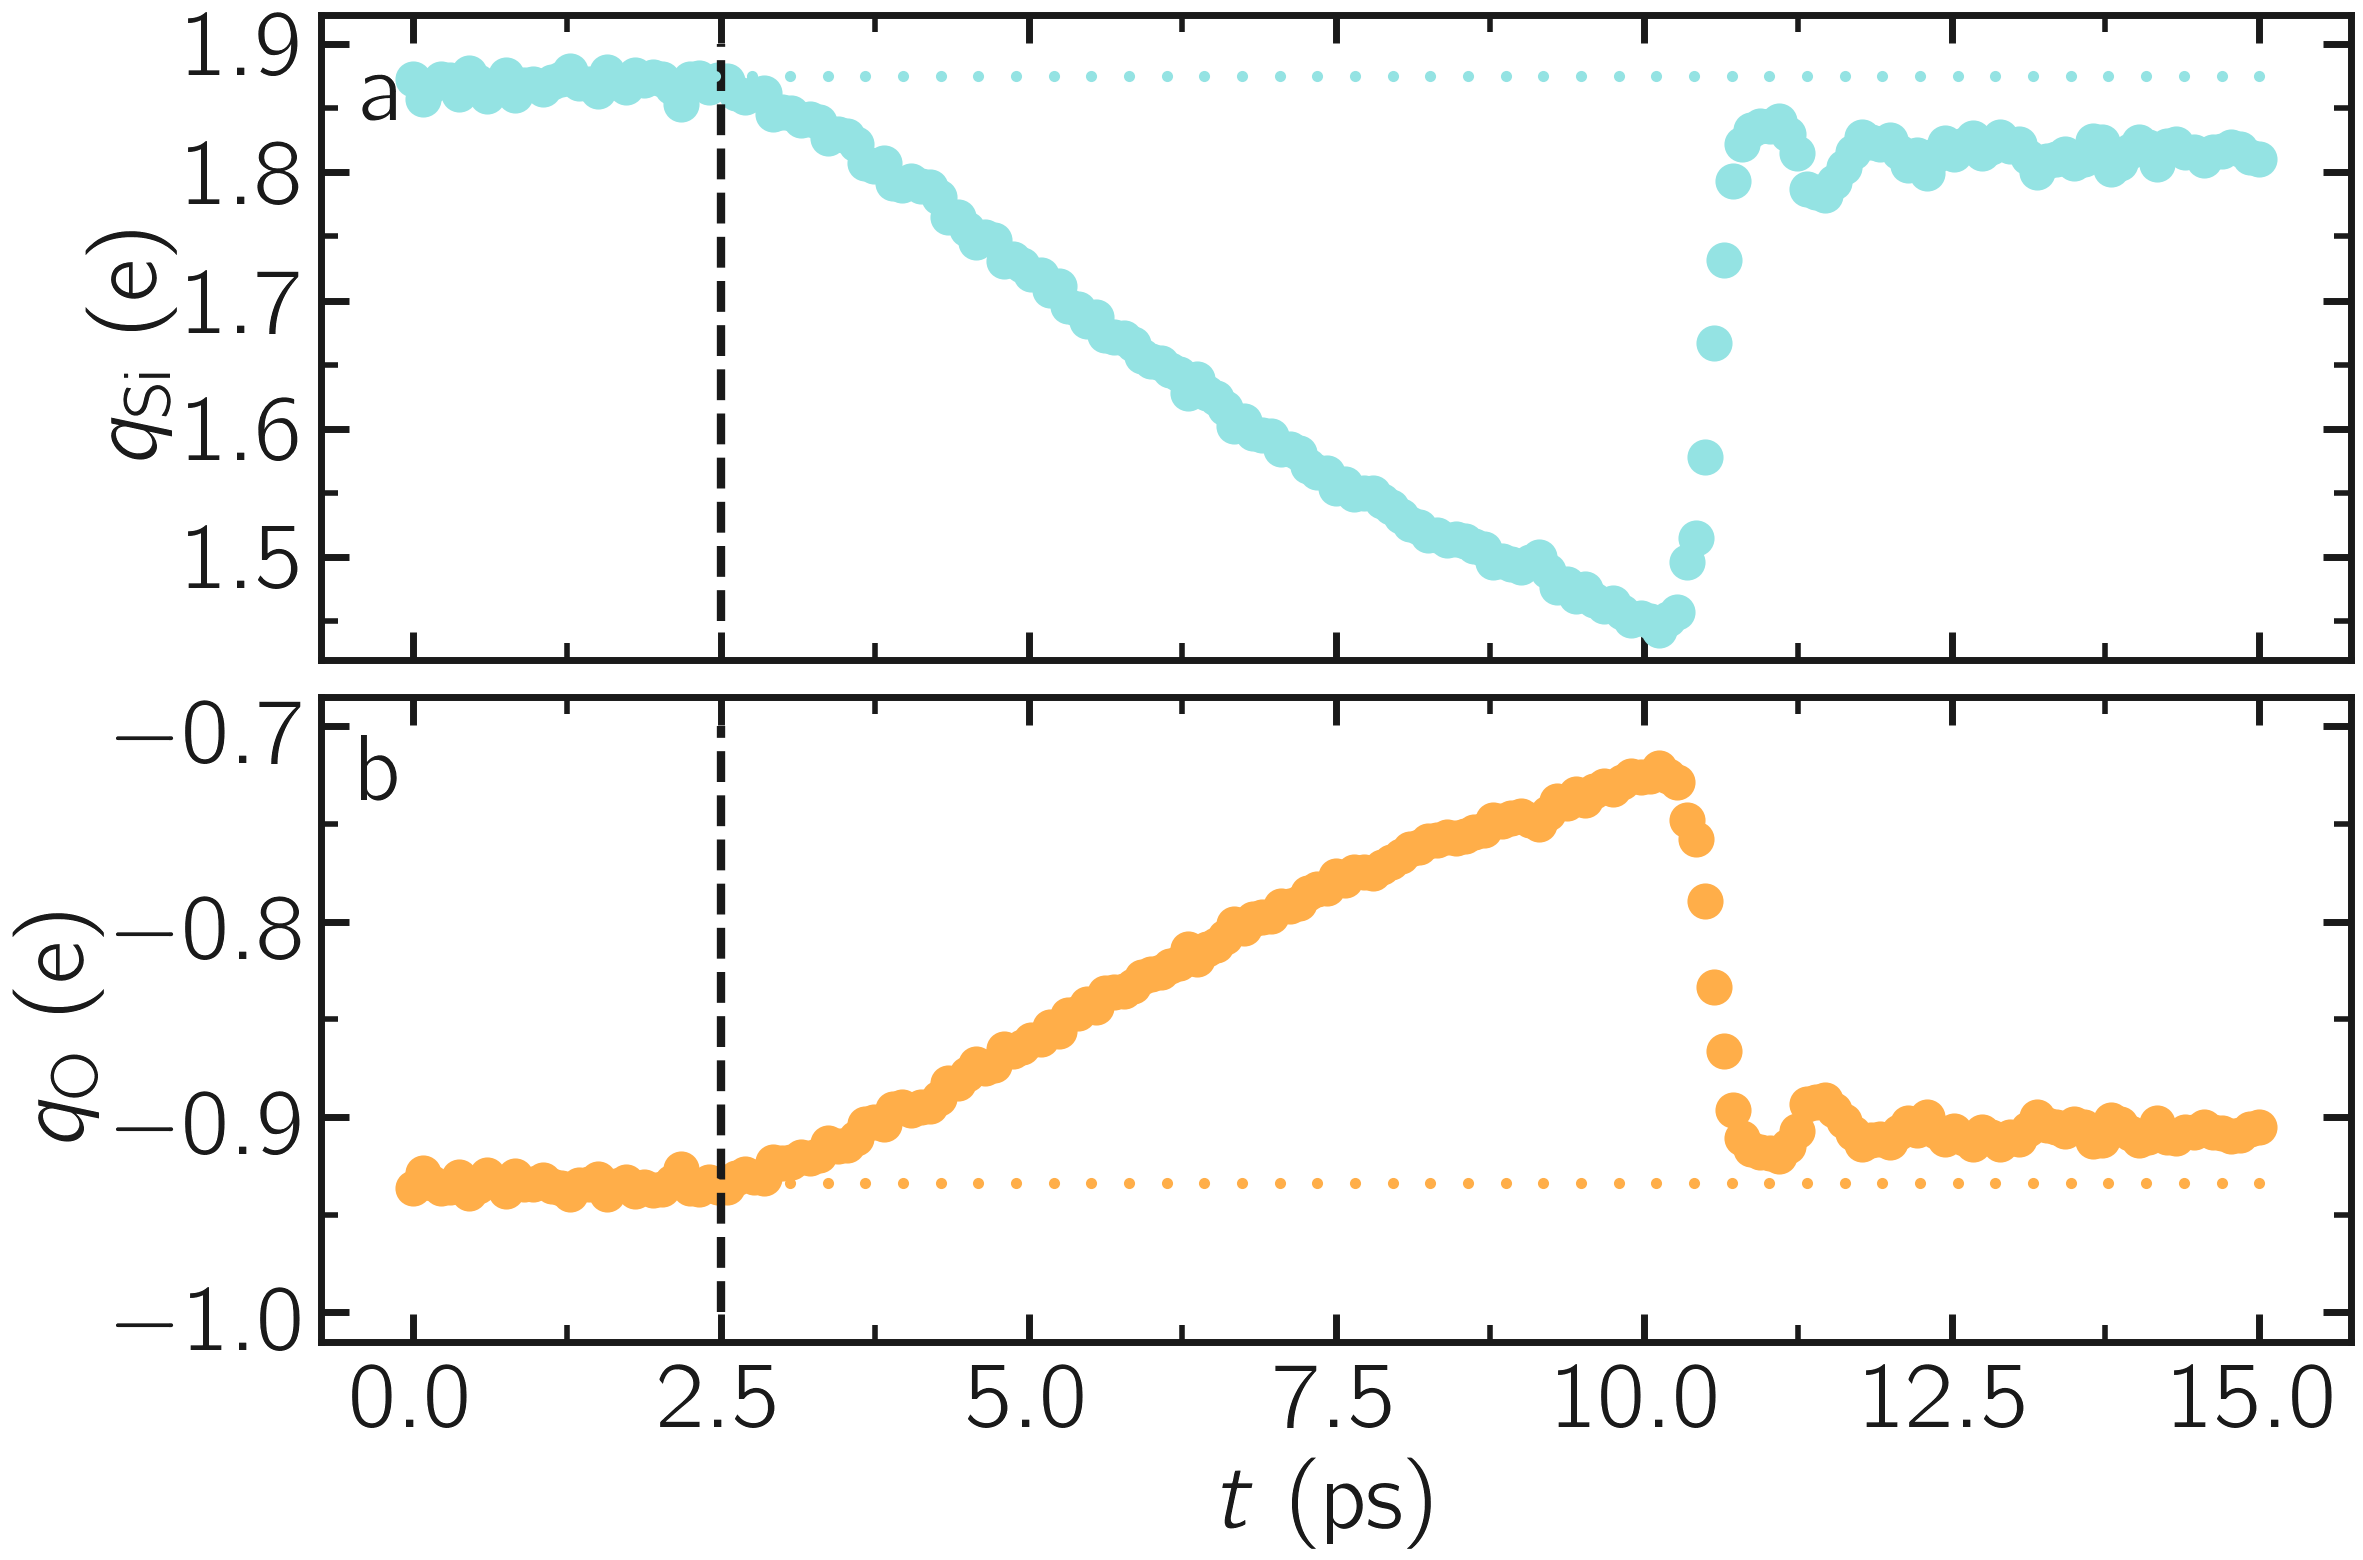
\includegraphics[width=\linewidth]{SIO-deformed-charge}
\caption{a) Average charge per atom of the silicon $q_\text{Si}$ atoms as
a function of time $t$ during deformation of the $\text{SiO}_2$ system
from \hyperref[reactive-silicon-dioxide-label]{Tutorial 5}.  b) Temperature $T$ of the
system as a function of time $t$.}
\label{fig:SIO-deformed-charge}
\end{figure}

Let us run for 5000 steps without deformation, then apply the \lmpcmd{fix deform}
to progressively elongate the box along the $x$-axis during 25000 steps.  Add
the following line to \flecmd{deform.lmp}:
\begin{lstlisting}
run 5000

fix mydef all deform 1 x erate 5e-5

run 25000

write_data deform.data
\end{lstlisting}
Run the \lmpcmd{deform.lmp} file using LAMMPS.  During the deformation, the charge
values progressively evolve until the structure eventually breaks down.  After the
structure breaks down, the charges equilibrate near new average values that differ
from the initial averages (Fig.~\ref{fig:SIO-deformed-charge}\,a).  The difference
between the initial and the final charges can be explained by the presence of
defects, as well as new solid/vacuum interfaces, and the fact that surface atoms
typically have different charges compared to bulk atoms (Fig.~\ref{fig:SIO-deformed}).
You can also see a sharp increase in temperature during the rupture of
the material (Fig.~\ref{fig:SIO-deformed-charge}\,b).

\begin{figure}
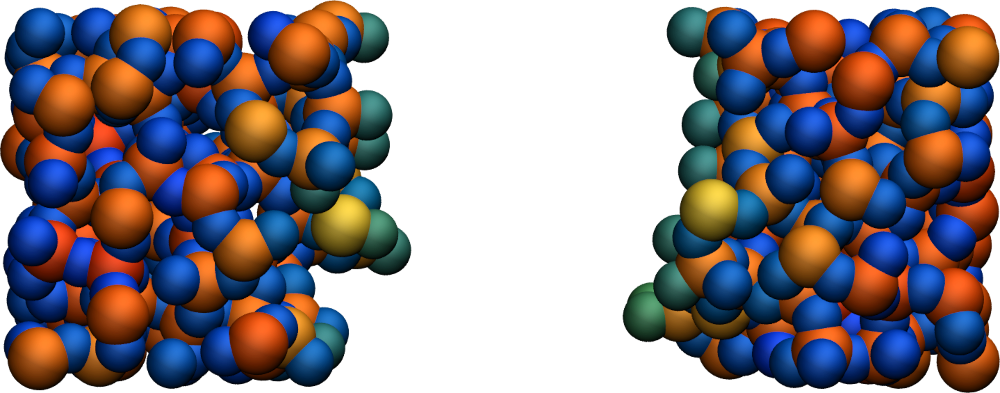
\includegraphics[width=\linewidth]{SIO-deformed}
\caption{Amorphous silicon oxide after deformation during
\hyperref[reactive-silicon-dioxide-label]{Tutorial 5}.  The atoms are colored by their
charges.  Dangling oxygen groups appear in greenish, bulk Si atoms with a charge of
about $1.8~\text{e}$  appear in red/orange, and bulk O atoms with a charge of
about $-0.9 ~ \text{e}$ appear in blue.}
\label{fig:SIO-deformed}
\end{figure}

You can examine the charge distribution after deformation, as well as during
deformation (Fig.~\ref{fig:SIO-distribution}\,b).  As expected, the final
charge distribution slightly differs from the previously calculated one.  If
no new species were formed during the simulation, the \flecmd{deform.species} file
should look like this:
\begin{lstlisting}
#  Timestep   No_Moles   No_Specs  O384Si192
        5            1          1          1
(...)
#  Timestep   No_Moles   No_Specs  O384Si192
    30000            1          1          1
\end{lstlisting}
Sometimes, $\text{O}_2$ molecules are formed during the deformation.  If this occurs,
a new column \lmpcmd{O2} appears in the \flecmd{deform.species} file.

\subsubsection{Decorate the surface}

Under ambient conditions, some of the surface $\text{SiO}_2$ atoms become chemically
passivated by forming covalent bonds with hydrogen (H) atoms~\cite{sulpizi2012silica}.
We will add hydrogen atoms randomly to the cracked silica and observe how the
system evolves.  To do so, we first need to modify the previously generated data
file \flecmd{deform.data} and make space for a third atom type.
Copy \flecmd{deform.data}, name the copy \flecmd{deform-mod.data}, and modify the
first lines of \flecmd{deform-mod.data} as follows:
\begin{lstlisting}
576 atoms
3 atom types

(...)

Atom Type Labels

1 Si
2 O
3 H

Masses

Si 28.0855
O 15.999
H 1.008

(...)
\end{lstlisting}

Open the \flecmd{decorate.lmp} file, which must contain the following lines:
\begin{lstlisting}
units real
atom_style full

read_data deform-mod.data
displace_atoms all move -12 0 0 # optional

pair_style reaxff NULL safezone 3.0 mincap 150
pair_coeff * * reaxCHOFe.inc Si O H
fix myqeq all qeq/reaxff 1 0.0 10.0 1.0e-6 reaxff maxiter 400
\end{lstlisting}
The \lmpcmd{displace\_atoms} command is used to move the center of the
crack near the center of the box.  This step is optional but makes for a nicer
visualization.  A different value for the shift may be needed in
your case, depending on the location of the crack.  A difference with the previous
input is that three atom types are specified in the \lmpcmd{pair\_coeff} command, i.e.
\lmpcmd{Si O H}.

Then, let us adapt some familiar commands to measure the charges of all three
types of atoms, and output the charge values into log files:
\begin{lstlisting}
group grpSi type Si
group grpO type O
group grpH type H
variable qSi equal charge(grpSi)/count(grpSi)
variable qO equal charge(grpO)/count(grpO)
variable qH equal charge(grpH)/(count(grpH)+1e-10)

thermo 5
thermo_style custom step temp etotal press v_qSi v_qO v_qH

dump viz all image 100 myimage-*.ppm q &
  type shiny 0.1 box no 0.01 view 180 90 zoom 2.3 size 1200 500
dump_modify viz adiam Si 2.6 adiam O 2.3 adiam H 1.0 &
  backcolor white amap -1 2 ca 0.0 3 min royalblue &
  0 green max orangered

fix myspec all reaxff/species 5 1 5 decorate.species &
  element Si O H
\end{lstlisting}
Here, the $+1 \mathrm{e}{-10}$ was added to the denominator of the \lmpcmd{variable qH}
to avoid dividing by 0 at the beginning of the simulation.  Finally, let us
create a loop with 10 steps, and create two hydrogen atoms at random locations at
every step:
\begin{lstlisting}
fix mynvt all nvt temp 300.0 300.0 100
timestep 0.5

label loop
variable a loop 10

variable seed equal 35672+${a}
create_atoms 3 random 2 ${seed} NULL overlap 2.6 maxtry 50

run 2000

next a
jump SELF loop
\end{lstlisting}
Run the simulation with LAMMPS.  When the simulation is over,
it can be seen from the \flecmd{decorate.species} file that
all the created hydrogen atoms reacted with the $\text{SiO}_{2}$ structure to
form surface groups (such as hydroxyl (-OH) groups).
\begin{lstlisting}
(...)
# Timestep   No_Moles No_Specs H20O384Si192
  20000      1        1        1
\end{lstlisting}
At the end of the simulation, hydroxyl (-OH) groups can be seen at the interfaces
(Fig.~\ref{fig:SIO-decorated}).

\begin{figure}
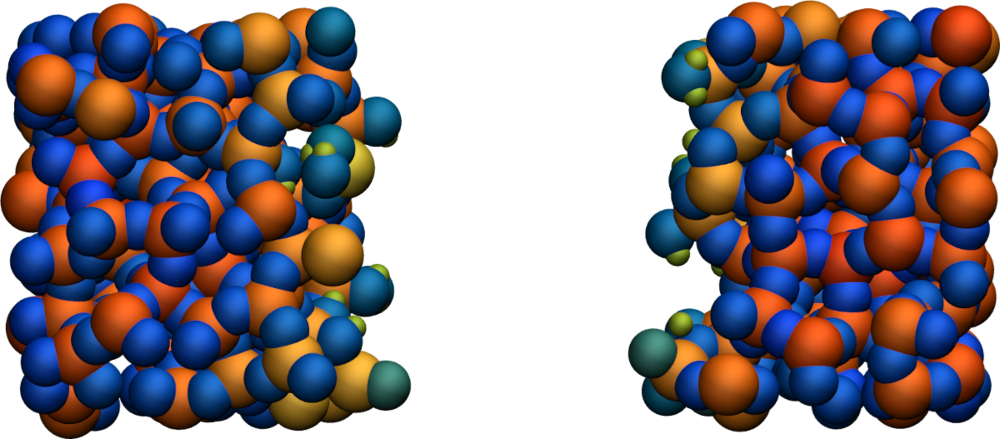
\includegraphics[width=\linewidth]{SIO-decorated}
\caption{Cracked silicon oxide after the addition of hydrogen atoms
during \hyperref[reactive-silicon-dioxide-label]{Tutorial 5}.  The atoms
are colored by their charges, with the newly added hydrogen atoms appearing as small
greenish spheres.}
\label{fig:SIO-decorated}
\end{figure}

\subsection{Tutorial 6: Water adsorption in silica}
\label{gcmc-silica-label}

\begin{figure}
\centering
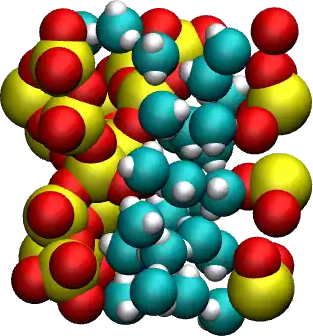
\includegraphics[width=0.6\linewidth]{GCMC}
\caption{Water molecules (H$_2$O) adsorbed in cracked silica (SiO$_2$) material as simulated
during \hyperref[gcmc-silica-label]{Tutorial 6}.  The oxygen atoms of the water
molecules are represented in cyan, the silicon atoms in yellow, and the oxygen
atoms of the solid in red.}
\label{fig:GCMC}
\end{figure}

\noindent The objective of this tutorial is to combine molecular dynamics and
grand canonical Monte Carlo simulations to compute the adsorption of water
molecules in cracked silica material (Fig.~\ref{fig:GCMC}).  This tutorial
illustrates the use of the grand canonical ensemble in molecular simulation, an
open ensemble where the number of atoms or molecules in the simulation box can vary.
By employing the grand canonical ensemble, we will set the chemical
potential of water within a nanoporous SiO$_2$ structure.

\subsubsection{Generation of the silica block}

\noindent To begin this tutorial, select \guicmd{Start Tutorial 6} from the
\guicmd{Tutorials} menu of \lammpsgui{} and follow the instructions.
The editor should display the following content corresponding to \flecmd{generate.lmp}:
\begin{lstlisting}
units metal
boundary p p p
atom_style full
pair_style vashishta
neighbor 1.0 bin
neigh_modify delay 1
\end{lstlisting}
The main difference from some of the previous tutorials is the use of the \lmpcmd{Vashishta}
pair style.  The Vashishta potential implicitly models atomic bonds through
energy terms dependent on interatomic distances and angles~\cite{vashishta1990interaction}.

Let us create a box for two atom types, \lmpcmd{Si}
of mass 28.0855\,g/mol and \lmpcmd{O} of mass 15.9994\,g/mol.
Add the following lines to \flecmd{generate.lmp}:
\begin{lstlisting}
region box block -18.0 18.0 -9.0 9.0 -9.0 9.0
create_box 2 box
labelmap atom 1 Si 2 O
mass Si 28.0855
mass O 15.9994
create_atoms Si random 240 5802 box overlap 2.0 maxtry 500
create_atoms O random 480 1072 box overlap 2.0 maxtry 500
\end{lstlisting}
The \lmpcmd{create\_atoms} commands are used to place
240 Si atoms, and 480 atoms, respectively.  This corresponds to
an initial density of approximately $2$\,g/cm$^3$, which is close
to the expected final density of amorphous silica at 300\,K.

Now, specify the pair coefficients by indicating that the first atom type
is \lmpcmd{Si} and the second is \lmpcmd{O}:
\begin{lstlisting}
pair_coeff * * SiO.1990.vashishta Si O
\end{lstlisting}
Ensure that the \href{\filepath tutorial6/SiO.1990.vashishta}{\dwlcmd{SiO.1990.vashishta}}
file is located in the same directory as \flecmd{generate.lmp}.

Next, add a \lmpcmd{dump image} command to \flecmd{generate.lmp} to follow the
evolution of the system with time:
\begin{lstlisting}
dump viz all image 250 myimage-*.ppm type type &
  shiny 0.1 box no 0.01 view 180 90 zoom 3.4 size 1700 700
dump_modify viz backcolor white &
  acolor Si yellow adiam Si 2.5 &
  acolor O red adiam O 2
\end{lstlisting}
Let us also print the box volume and system density, alongside the
temperature and total energy:
\begin{lstlisting}
thermo 250
thermo_style custom step temp etotal vol density
\end{lstlisting}

Finally, let us implement the annealing procedure which
consists of three consecutive runs.  This procedure was inspired
by Ref.\,\cite{della1992molecular}.  First, to melt the system,
a $10\,\text{ps}$ phase at $T = 6000\,\text{K}$ is performed:
\begin{lstlisting}
velocity all create 6000 8289 rot yes dist gaussian
fix mynvt all nvt temp 6000 6000 0.1
timestep 0.001
run 10000
\end{lstlisting}
Next, a second phase, during which the system is cooled down from $T = 6000\,\text{K}$
to $T = 300\,\text{K}$, is implemented as follows:
\begin{lstlisting}
fix mynvt all nvt temp 6000 300 0.1
run 30000
\end{lstlisting}
In the third step, the system is equilibrated at the final desired
conditions, $T = 300\,\text{K}$ and $p = 1\,\text{atm}$,
using an anisotropic pressure coupling:
\begin{lstlisting}
unfix mynvt

fix mynpt all npt temp 300 300 0.1 aniso 1 1 1
run 10000

write_data generate.data
\end{lstlisting}
Here, an anisotropic barostat is used.
Anisotropic barostats adjust the dimensions independently, which is
generally suitable for a solid phase.

Run the simulation using LAMMPS.  From the \guicmd{Charts} window, the temperature
evolution can be observed, showing that it closely follows the desired annealing procedure (Fig.~\ref{fig:GCMC-dimension}\,a).
The evolution of the box dimensions over time confirms that the box
deformed during the last stage of the simulation
(Fig.~\ref{fig:GCMC-dimension}\,b).  After the simulation completes, the final
LAMMPS topology file called \flecmd{generate.data}
will be located next to \flecmd{generate.lmp} (Fig.~\ref{fig:GCMC-snapshot}).

\begin{figure}
\centering
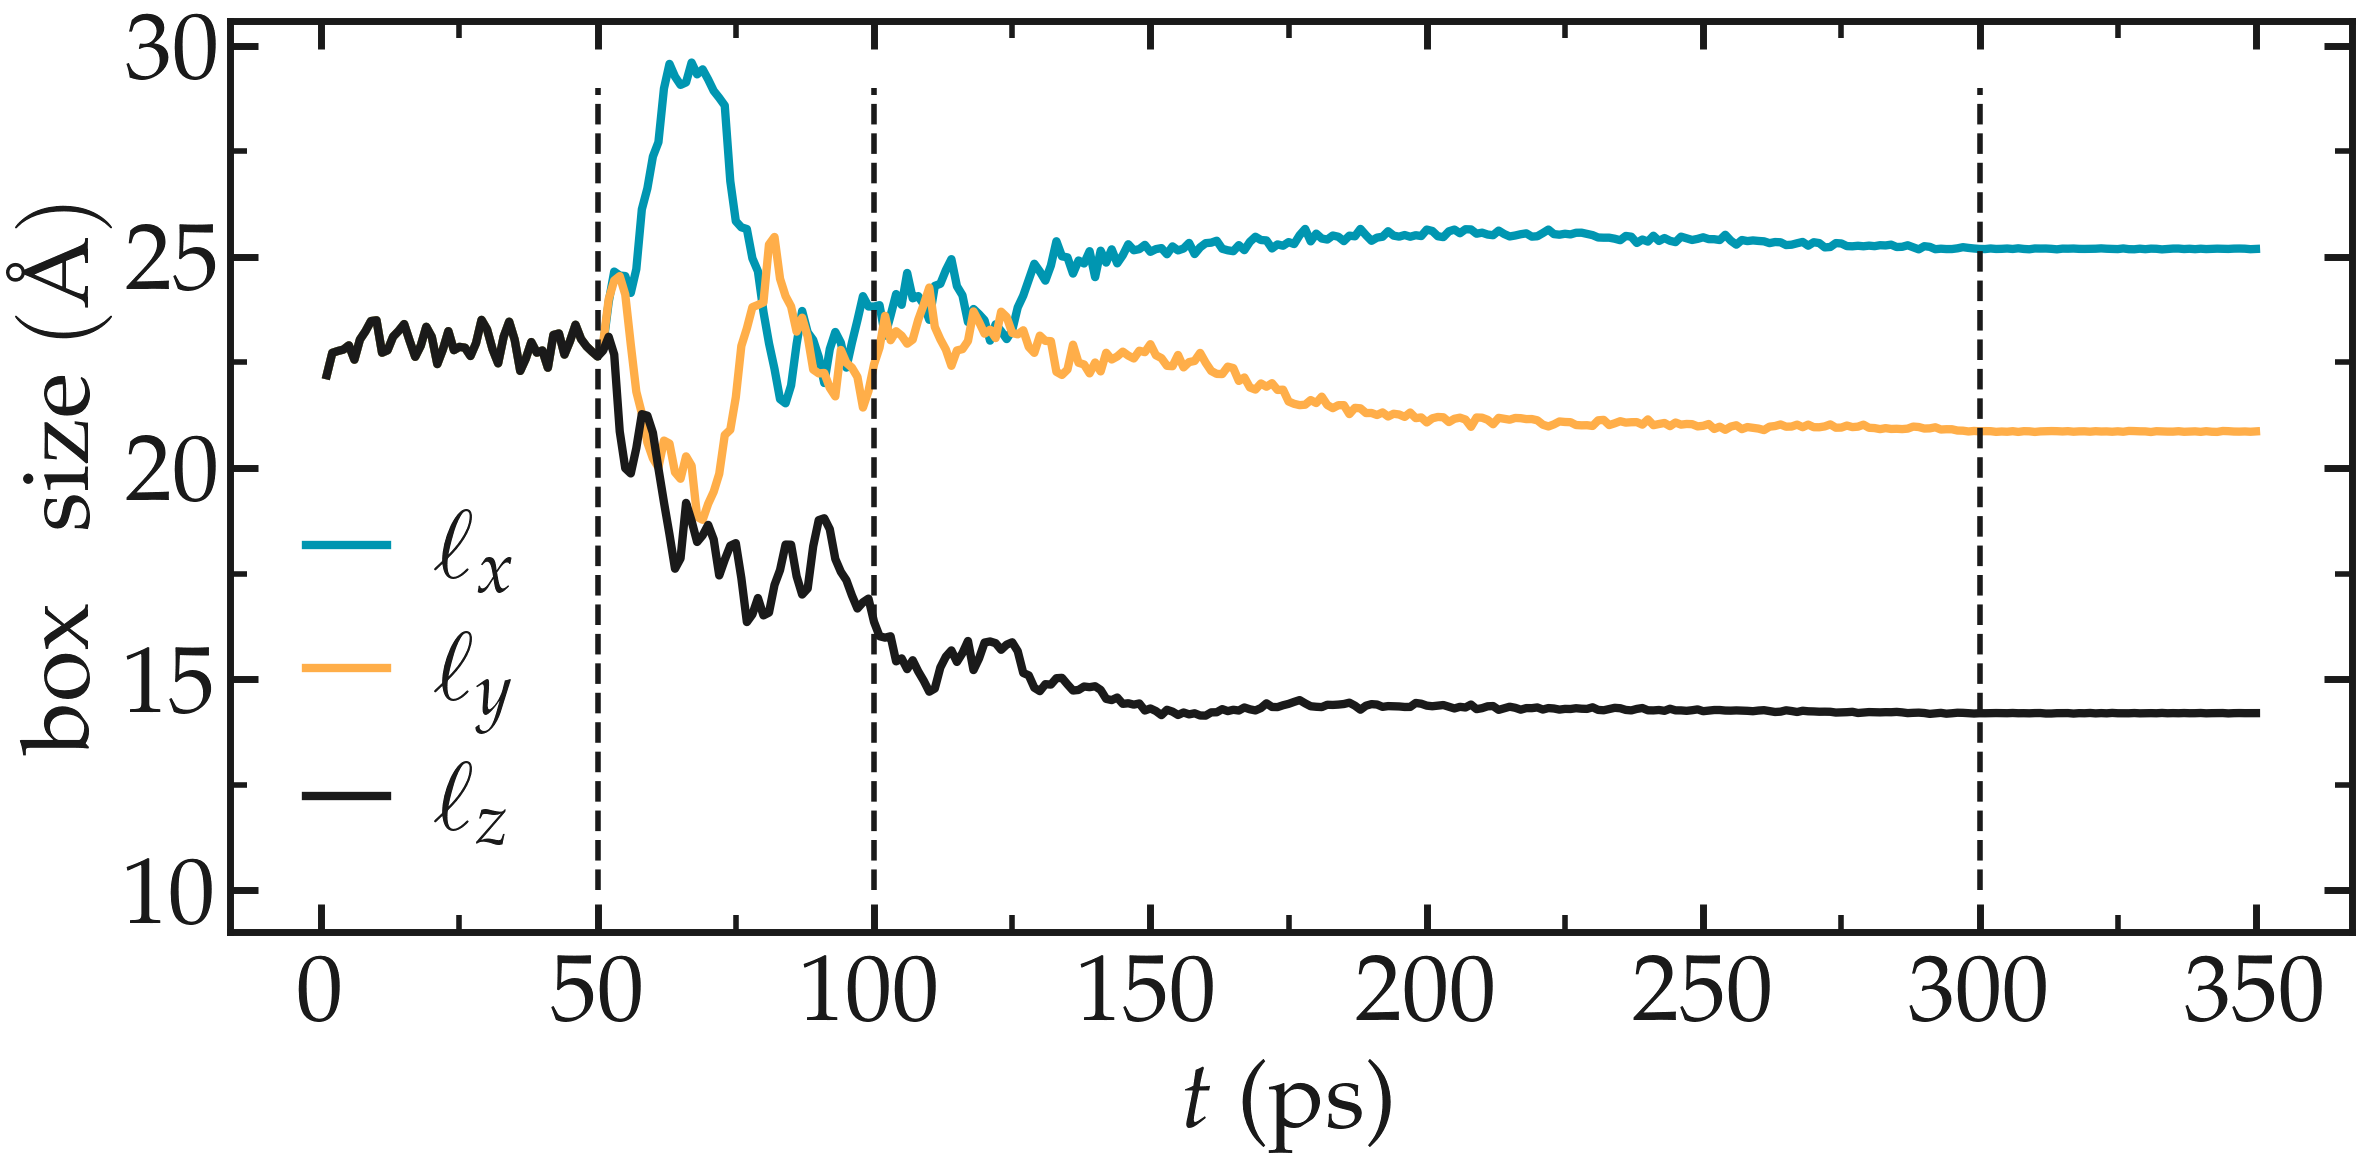
\includegraphics[width=\linewidth]{GCMC-dimension}
\caption{a) Temperature $T$ as a function of time $t$ during the annealing
of the silica system from \hyperref[gcmc-silica-label]{Tutorial 6}.
b) System density $\rho$ during the annealing process.  The vertical dashed lines
mark the transition between the different phases of the simulation.}
\label{fig:GCMC-dimension}
\end{figure}

\begin{figure}
\centering
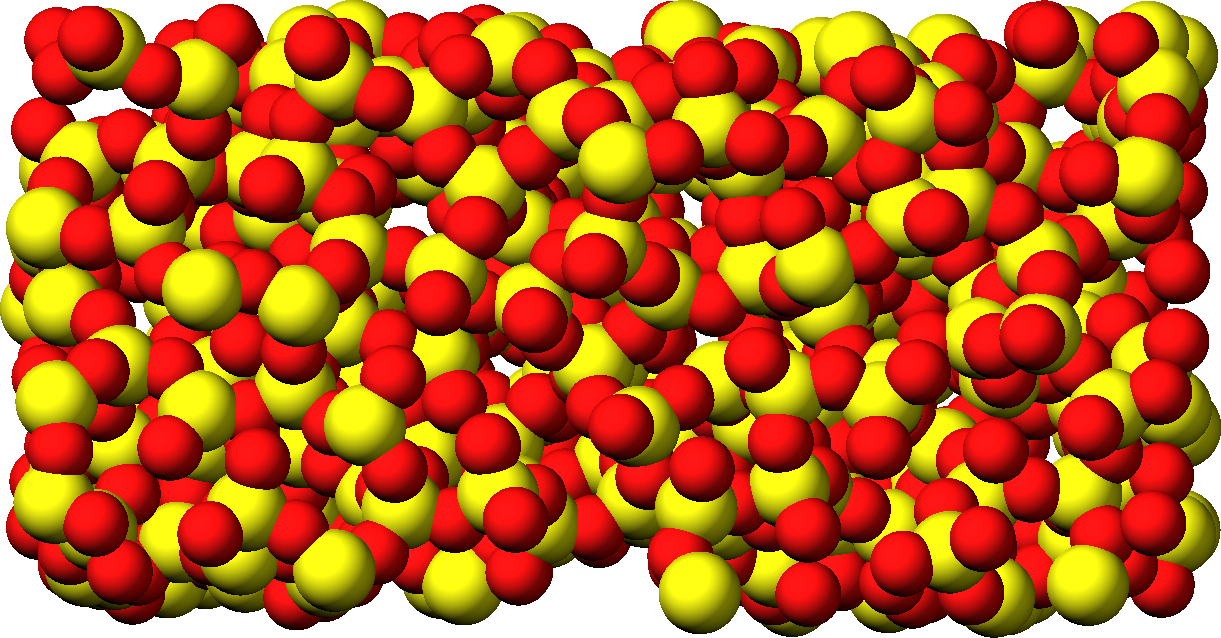
\includegraphics[width=0.9\linewidth]{GCMC-generate}
\caption{Amorphous silica ($\text{SiO}_2$) simulated
during \hyperref[gcmc-silica-label]{Tutorial 6}.  Silicon atoms are
represented in yellow, and oxygen atoms in red.}
\label{fig:GCMC-snapshot}
\end{figure}

\subsubsection{Cracking the silica}

Open the \flecmd{cracking.lmp} file, which must contain the following familiar lines:
\begin{lstlisting}
units metal
boundary p p p
atom_style full
pair_style vashishta
neighbor 1.0 bin
neigh_modify delay 1

read_data generate.data

pair_coeff * * SiO.1990.vashishta Si O

dump viz all image 250 myimage-*.ppm type type &
  shiny 0.1 box no 0.01 view 180 90 zoom 3.4 size 1700 700
dump_modify viz backcolor white &
  acolor Si yellow adiam Si 2.5 &
  acolor O red adiam O 2

thermo 250
thermo_style custom step temp etotal vol density
\end{lstlisting}

Let us progressively increase the size of the box in the $x$ direction,
forcing the silica to deform and eventually crack.  To achive this,
the \lmpcmd{fix deform} command is used, with a rate
of $0.005\,\text{ps}^{-1}$.  Add the following lines to
the \flecmd{cracking.lmp} file:
\begin{lstlisting}
timestep 0.001
fix nvt1 all nvt temp 300 300 0.1
fix mydef all deform 1 x erate 0.005
run 50000

write_data cracking.data
\end{lstlisting}
The \lmpcmd{fix nvt} command is employed to control the temperature of the system.
As observed from the generated images, the atoms
progressively adjust to the changing box dimensions.  At some point,
bonds begin to break, leading to the appearance of
dislocations (Fig.~\ref{fig:GCMC-cracked}).

\begin{figure}
\centering
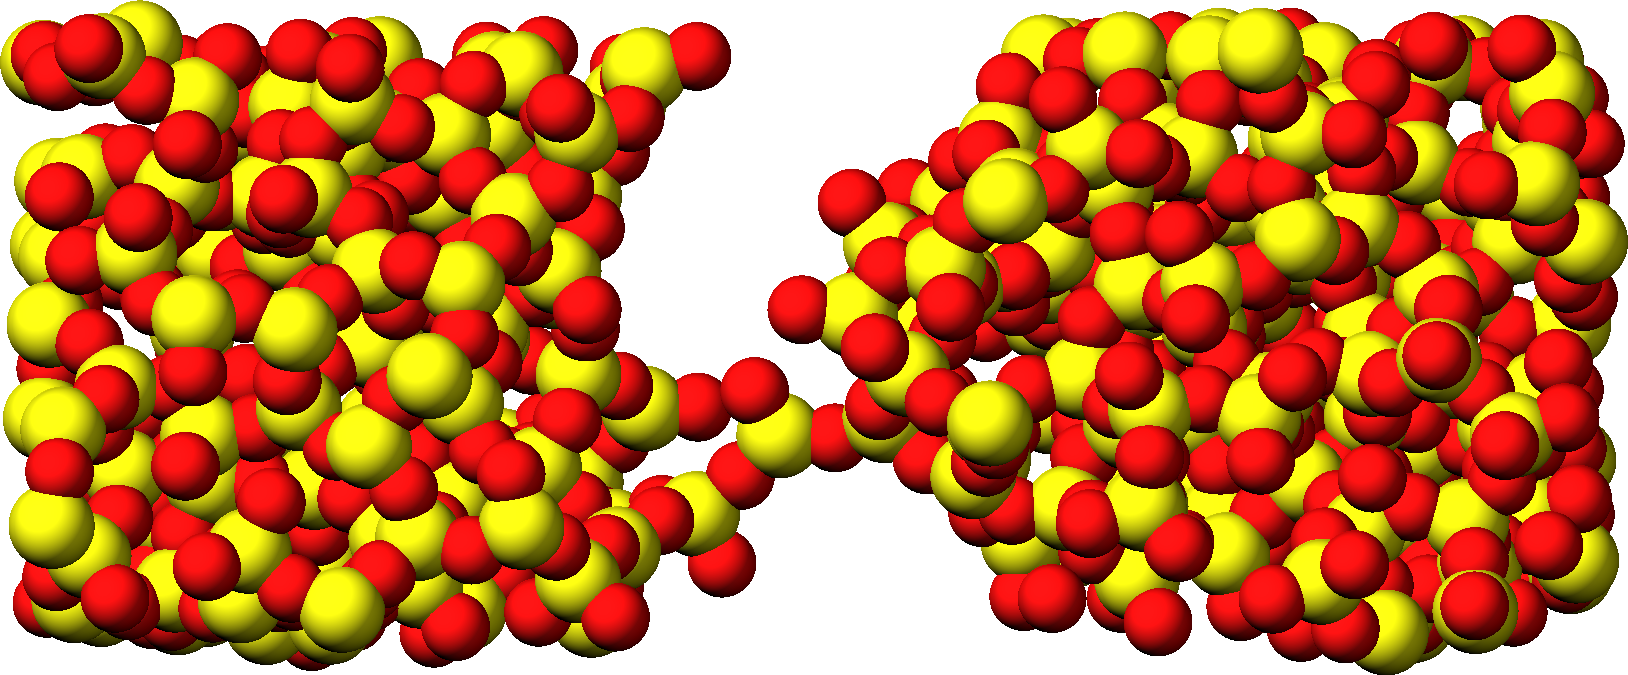
\includegraphics[width=\linewidth]{GCMC-cracked}
\caption{Block of silica from \hyperref[gcmc-silica-label]{Tutorial 6}
after deformation.  Silicon atoms are represented in yellow,
and oxygen atoms in red.  The crack was induced by the
imposed deformation of the box along the $x$-axis (i.e.,~the horizontal axis).}
\label{fig:GCMC-cracked}
\end{figure}

\subsubsection{Adding water}

\noindent To add the water molecules to the silica, we will employ
the Monte Carlo method in the grand canonical ensemble (GCMC).  In short, the
system is placed into contact with a virtual reservoir of a given chemical potential
$\mu$, and multiple attempts to insert water molecules at random positions are
made.  Each attempt is either accepted or rejected based on energy considerations.
For further details, please refer to classical textbooks like Ref.~\citenum{frenkel2023understanding}.

\paragraph{Using hydrid potentials}

\noindent The first particularly of our system is that it
combine water and silica, which necessitates the use
of two force fields: Vashishta (for $\text{SiO}_2$), and
TIP4P (for water).  Here, the TIP4P/2005 model is employed for the
water~\cite{abascal2005general}.  Open the \flecmd{gcmc.lmp} file, which
should contain the following lines:
\begin{lstlisting}
units metal
boundary p p p
atom_style full
neighbor 1.0 bin
neigh_modify delay 1
pair_style hybrid/overlay vashishta &
    lj/cut/tip4p/long OW HW OW-HW HW-OW-HW 0.1546 10
kspace_style pppm/tip4p 1.0e-5
bond_style harmonic
angle_style harmonic
\end{lstlisting}
Combining the two force fields, Vashishta and TIP4P/2005, is achieved
using the \lmpcmd{hybrid/overlay} pair style.  The PPPM
solver~\cite{luty1996calculating} is specified with the \lmpcmd{kspace}
command, and is used to compute the long-range Coulomb interactions associated
with \lmpcmd{tip4p/long}.  Finally, the style for the bonds
and angles of the water molecules are defined; however, these specifications are
not critical since TIP4P/2005 is a rigid water model.

The water molecule template called \href{\filepath tutorial6/H2O.mol}{\dwlcmd{H2O.mol}}
must be downloaded and located next to \flecmd{gcmc.lmp}

Before going further, we need to make a few changes to our data file.
Currently, the \flecmd{cracking.data} file includes only two atom types, but we require four.
Copy the previously generated \flecmd{cracking.data}, and name the duplicate \flecmd{cracking-mod.data}.
Make the following changes to the beginning of \flecmd{cracking-mod.data}
to ensure it matches the following format (with 4 atom types,
1 bond type, 1 angle type, the proper type labels, and four masses):
\begin{lstlisting}
720 atoms
4 atom types
1 bond types
1 angle types

2 extra bond per atom
1 extra angle per atom
2 extra special per atom

-22.470320800269317 22.470320800269317 xlo xhi
-8.579178758211475 8.579178758211475 ylo yhi
-8.491043517346204 8.491043517346204 zlo zhi

Atom Type Labels

1 Si
2 O
3 OW
4 HW

Bond Type Labels

1 OW-HW

Angle Type Labels

1 HW-OW-HW

Masses

1 28.0855
2 15.9994
3 15.9994
4 1.008

Atoms # full

(...)
\end{lstlisting}
Doing so, we anticipate that there will be 4 atom types in the simulations,
with the oxygens and hydrogens of $\text{H}_2\text{O}$ having
types \lmpcmd{OW} and \lmpcmd{HW}, respectively.  There
will also be 1 bond type (\lmpcmd{OW-HW}) and 1 angle type (\lmpcmd{OW-HW-HW}).
The \lmpcmd{extra bond}, \lmpcmd{extra angle}, and
\lmpcmd{extra special} lines are here for memory allocation.

We can now proceed to complete the \flecmd{gcmc.lmp} file by adding the system definition:
\begin{lstlisting}
read_data cracking-mod.data
molecule h2omol H2O.mol
create_atoms 0 random 3 3245 NULL mol h2omol 4585 &
  overlap 2.0 maxtry 50

group SiO type Si O
group H2O type OW HW
\end{lstlisting}
After reading the data file and defining the \lmpcmd{h2omol} molecule from the \flecmd{H2O.txt}
file, the \lmpcmd{create\_atoms} command is used to include three water molecules
in the system.  Then, add the following \lmpcmd{pair\_coeff} (and
\lmpcmd{bond\_coeff} and \lmpcmd{angle\_coeff}) commands
to \flecmd{gcmc.lmp}:
\begin{lstlisting}
pair_coeff * * vashishta SiO.1990.vashishta Si O NULL NULL
pair_coeff * * lj/cut/tip4p/long 0 0
pair_coeff Si OW lj/cut/tip4p/long 0.0057 4.42
pair_coeff O OW lj/cut/tip4p/long 0.0043 3.12
pair_coeff OW OW lj/cut/tip4p/long 0.008 3.1589
pair_coeff HW HW lj/cut/tip4p/long 0.0 0.0
bond_coeff OW-HW 0 0.9572
angle_coeff HW-OW-HW 0 104.52
\end{lstlisting}
The force field Vashishta applies only to \lmpcmd{Si} and \lmpcmd{O} of $\text{SiO}_2$,
and not to the \lmpcmd{OW} and \lmpcmd{HW} of $\text{H}_2\text{O}$, thanks to the \lmpcmd{NULL} parameters
used for atoms of types \lmpcmd{OW} and \lmpcmd{HW}.  Pair coefficients for the \lmpcmd{lj/cut/tip4p/long}
potential are defined between O($\text{H}_2\text{O}$) and between H($\text{H}_2\text{O}$)
atoms, as well as between O($\text{SiO}_2$)-O($\text{H}_2\text{O}$) and
Si($\text{SiO}_2$)-O($\text{H}_2\text{O}$). Thus,  the fluid-fluid and the
fluid-solid interactions will be adressed with by the \lmpcmd{lj/cut/tip4p/long} potential.
The \lmpcmd{bond\_coeff} and \lmpcmd{angle\_coeff} commands set the \lmpcmd{OW-HW}
bond length to 0.9572\,\AA, and the \lmpcmd{HW-OW-HW}
angle to $104.52^\circ$, respectively~\cite{abascal2005general}.

Add the following lines to \flecmd{gcmc.lmp} as well:
\begin{lstlisting}
variable oxygen atom type==label2type(atom,OW)
group oxygen dynamic all var oxygen
variable nO equal count(oxygen)

fix shak H2O shake 1.0e-5 200 0 b OW-HW &
  a HW-OW-HW mol h2omol
\end{lstlisting}
The number of oxygen atoms from water molecules (i.e.~the number of molecules)
is calculated by the \lmpcmd{nO} variable.  The SHAKE algorithm is used to
maintain the shape of the water molecules over time~\cite{ryckaert1977numerical, andersen1983rattle}.

Finally, let us create images
of the system using \lmpcmd{dump image}:
\begin{lstlisting}
dump viz all image 250 myimage-*.ppm type type &
  shiny 0.1 box no 0.01 view 180 90 zoom 3.4 size 1700 700
dump_modify viz backcolor white &
  acolor Si yellow adiam Si 2.5 &
  acolor O red adiam O 2 &
  acolor OW cyan adiam OW 2 &
  acolor HW white adiam HW 1
\end{lstlisting}

\paragraph{GCMC simulation}

To prepare for the GCMC simulation, let us add the
following lines into \flecmd{gcmc.lmp}:
\begin{lstlisting}
compute ctH2O H2O temp
compute_modify thermo_temp dynamic yes
compute_modify ctH2O dynamic yes
fix mynvt1 H2O nvt temp 300 300 0.1
fix_modify mynvt1 temp ctH2O
fix mynvt2 SiO nvt temp 300 300 0.1
timestep 0.001
\end{lstlisting}
Two different thermostats are used for $\text{SiO}_2$ and $\text{H}_2\text{O}$,
respectively.  Using separate thermostats is usually better when the system contains
two separate species, such as a solid and a liquid.  It is particularly important
to use two thermostats here because the number of water molecules will fluctuate
with time.  The \lmpcmd{compute\_modify} command with the \lmpcmd{dynamic yes}
option for water is used to specify that the number of molecules will not be constant.

Finally, let us use the \lmpcmd{fix gcmc} and perform the grand canonical Monte
Carlo steps.  Add the following lines into \flecmd{gcmc.lmp}:
\begin{lstlisting}
variable tfac equal 5.0/3.0
fix fgcmc H2O gcmc 100 100 0 0 65899 300 -0.5 0.1 &
  mol h2omol tfac_insert ${tfac} shake shak &
  full_energy pressure 100
\end{lstlisting}
The \lmpcmd{tfac\_insert} option ensures the correct estimate for the temperature
of the inserted water molecules by taking into account the internal degrees of
freedom.  Here, 100 insertion and deletion attemps are made every 100 steps.

\begin{note}
At a pressure of $p = 100\ \text{bar}$, the chemical potential of water vapor at $T = 300\ \text{K}$
can be calculated using as $\mu = \mu_0 + RT \ln (\frac{p}{p_0}),$ where $\mu_0$ is the standard
chemical potential (typically taken at a pressure $p_0 = 1 \, \text{bar}$), \(R = 8.314\ \text{J/mol·K}\)
is the gas constant, \(T = 300\ \text{K}\) is the temperature.
\end{note}

Finally, let us print some information and run for 25\,ps:
\begin{lstlisting}
thermo 250
thermo_style custom step temp etotal v_nO &
  f_fgcmc[3] f_fgcmc[4] f_fgcmc[5] f_fgcmc[6]

run 25000
\end{lstlisting}
Running this simulation using LAMMPS, one can see that the number of molecules is increasing
progressively.  When using the pressure argument, LAMMPS ignores the value of the
chemical potential (here $\mu = -0.5\,\text{eV}$, which corresponds roughly to
ambient conditions, i.e.~to a relative humidity $\text{RH} \approx 50\,\%$~\cite{gravelle2020multi}.)
The large pressure value of 100\,bars was chosen to ensure that some successful
insertions of molecules would occur during the short duration of this simulation.

\begin{figure}
\centering
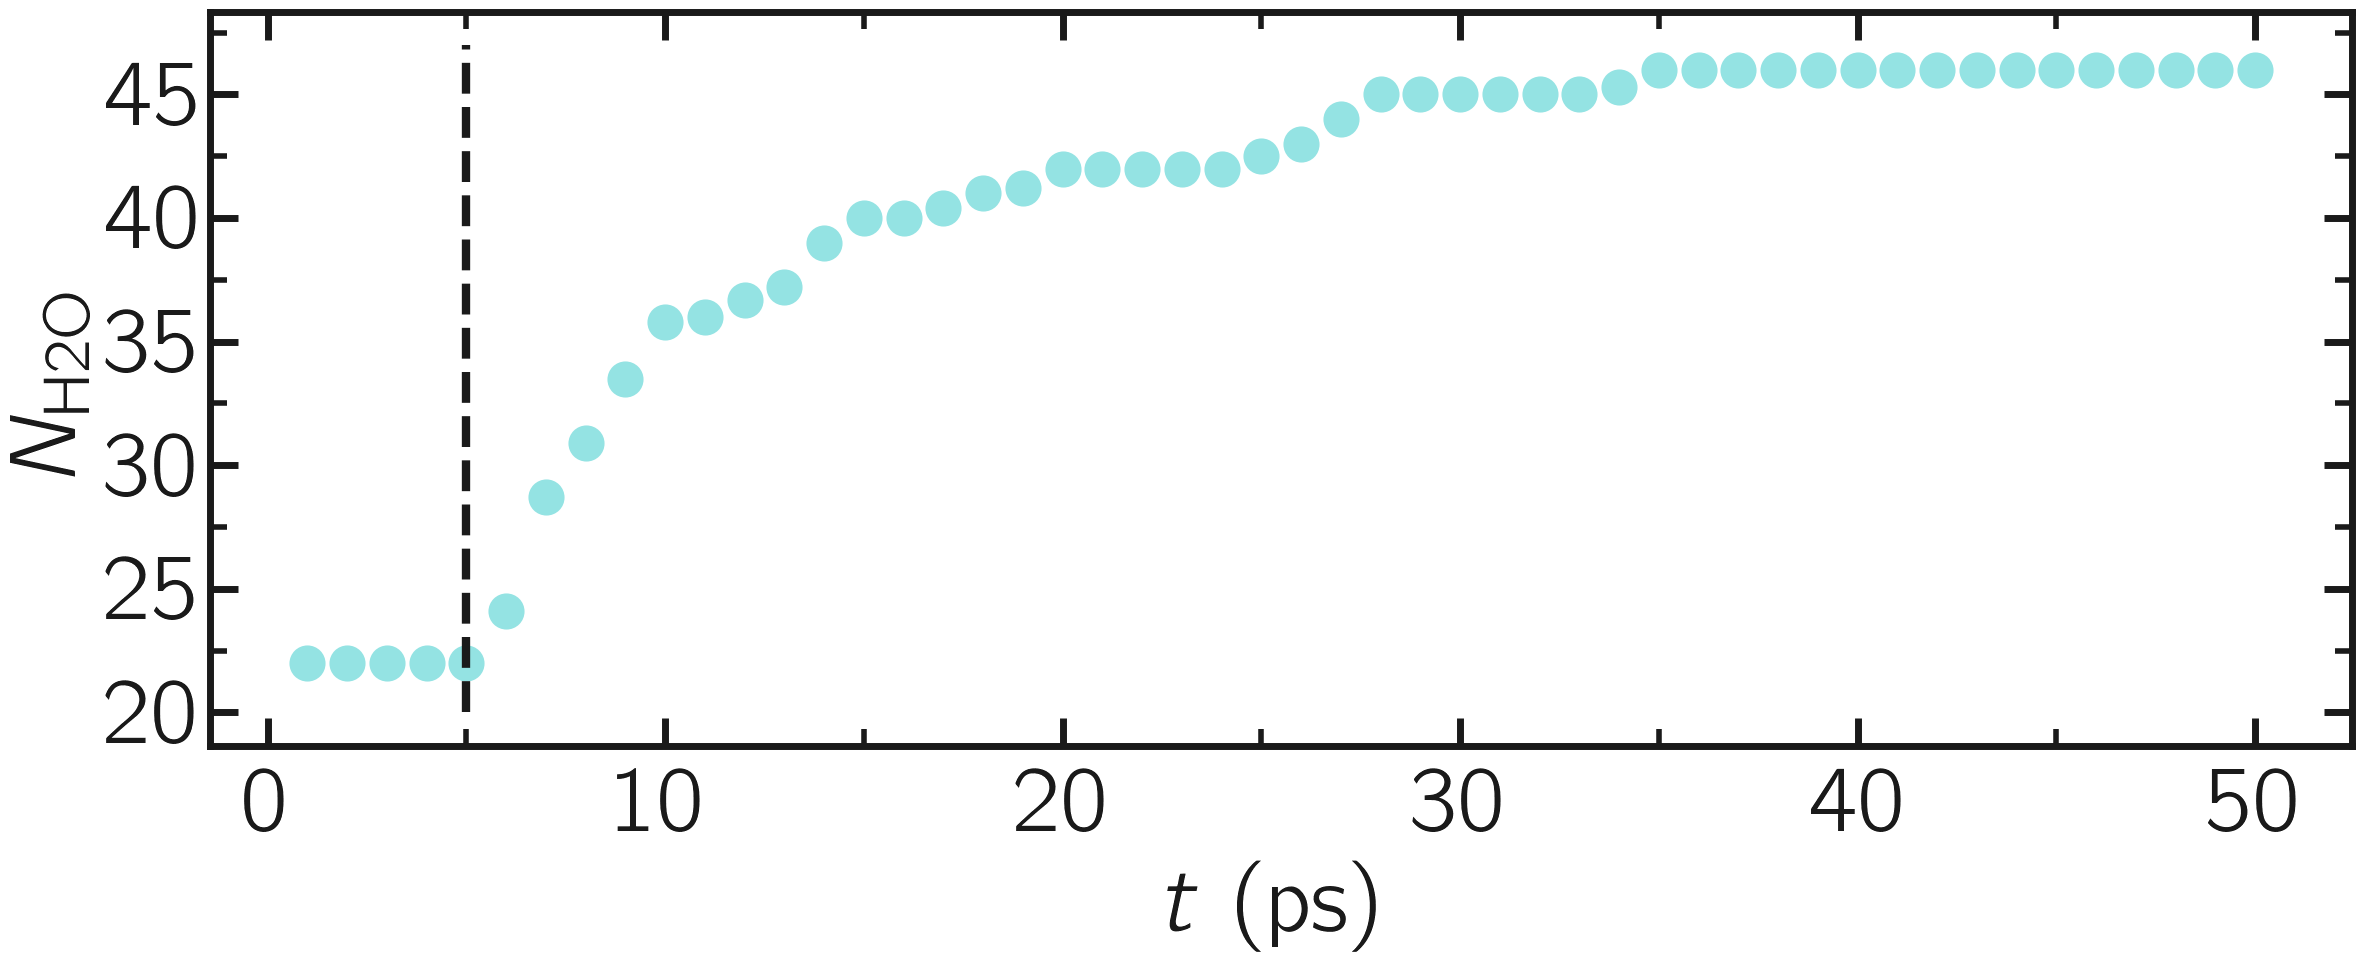
\includegraphics[width=\linewidth]{GCMC-number}
\caption{Number of water molecules, $N_\text{H2O}$, as a function of time, $t$,
as extracted from \hyperref[gcmc-silica-label]{Tutorial 6}.}
\label{fig:GCMC-number}
\end{figure}

After a few GCMC steps, the number of molecules starts increasing.  Once the
crack is filled with water molecules, the total number of molecules reaches a plateau
(Figs.\,\ref{fig:GCMC-number}-\ref{fig:GCMC-solvated}).  The final number of
molecules depends on the imposed pressure, temperature, and the interaction
between water and silica (i.e.~its hydrophilicity).  Note that GCMC simulations
of such dense phases are usually slow to converge due to the very low probability
of successfully inserting a molecule.  Here, the short simulation duration was
made possible by the use of a high pressure.

\begin{figure}
\centering
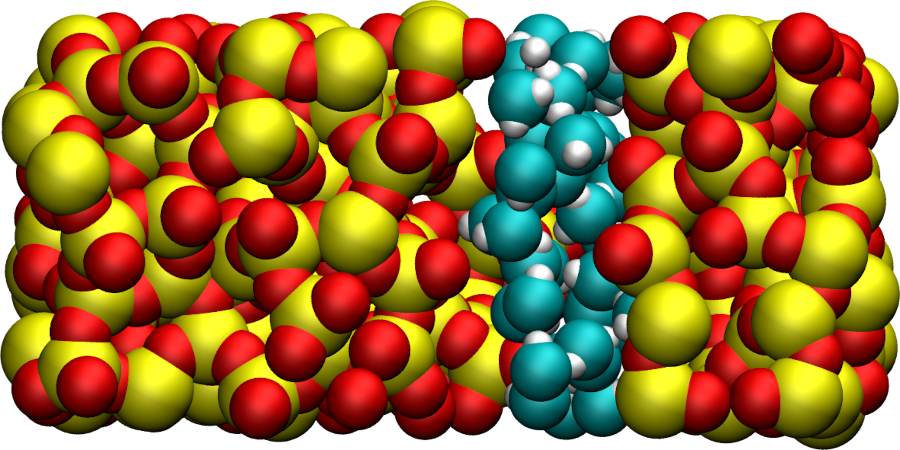
\includegraphics[width=\linewidth]{GCMC-solvated}
\caption{Snapshot of the silica system after the adsorption of water molecules
during \hyperref[gcmc-silica-label]{Tutorial 6}.
The oxygen atoms of the water molecules are represented in cyan, the silicon
atoms in yellow, and the oxygen atoms of the solid in red.}
\label{fig:GCMC-solvated}
\end{figure}

\subsection{Tutorial 7: Free energy calculation}
\label{umbrella-sampling-label}

\begin{figure}
\centering
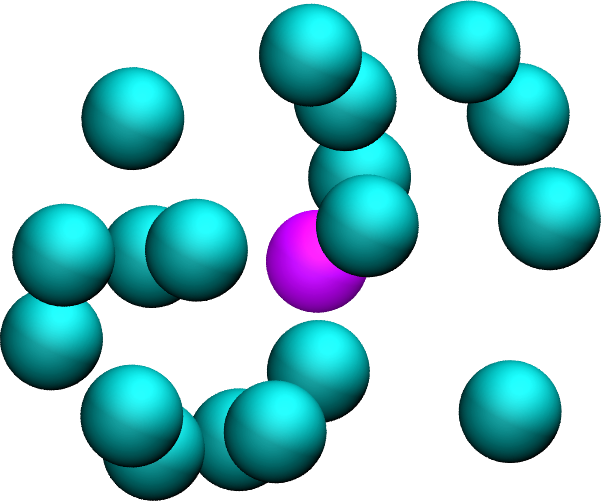
\includegraphics[width=0.7\linewidth]{US}
\caption{System simulated during \hyperref[umbrella-sampling-label]{Tutorial 7}.
The pink atom explores the energetically unfavorable central area of the simulation
box thanks to the additional potential imposed during umbrella sampling.}
\label{fig:US}
\end{figure}

\noindent The objective of this tutorial is to measure the free energy profile
of particles through a barrier potential using two methods: free sampling and
umbrella sampling~\cite{kastner2011umbrella, allen2017computer, frenkel2023understanding} (Fig.~\ref{fig:US}).
To simplify the process and minimize computation time, the barrier potential will be
imposed on the atoms using an additional force, mimicking the presence of a repulsive
area in the middle of the simulation box without needing to simulate additional atoms.
The procedure is valid for more complex systems and can be adapted to many other
situations, such as measuring adsorption barriers near an interface or calculating
translocation barriers through a membrane~\cite{wilson1997adsorption, makarov2009computer,
gravelle2021adsorption, loche2022molecular, hayatifar2024probing}.

\subsubsection{Method 1: Free sampling}
The most direct way to calculate a free energy profile is to extract the partition
function from a classical (i.e.~unbiased) molecular dynamics simulation, and
then estimate the Gibbs free energy by using
\begin{equation}
\Delta G = -RT \ln(p/p_0),
\label{eq:G}
\end{equation}
where $\Delta G$ is the free energy difference, $R$ is the gas constant, $T$
is the temperature, $p$ is the pressure, and $p_0$ is a reference pressure.
As an illustration, let us apply this method to a simple configuration
that consists of a particles in a box in the presence of a
position-dependent repulsive force that makes the center of the box a less
favorable area to explore.

\paragraph{Basic LAMMPS parameters}

To begin this tutorial, select \guicmd{Start Tutorial 7} from the
\guicmd{Tutorials} menu of \lammpsgui{} and follow the instructions.
The editor should display the following content corresponding to \flecmd{free-energy.lmp}:
\begin{lstlisting}
variable sigma equal 3.405
variable epsilon equal 0.238
variable U0 equal 1.5*${epsilon}
variable dlt equal 1.0
variable x0 equal 10.0

units real
atom_style atomic
pair_style lj/cut 3.822
pair_modify shift yes
boundary p p p
\end{lstlisting}
Here, we begin by defining variables for the Lennard-Jones interaction
$\sigma$ and $\epsilon$ and for the repulsive potential $U$, which are $U_0$, $\delta$, and $x_0$
[see Eqs.\,(\ref{eq:U}-\ref{eq:F}) below].  The cut-off value of 3.822 was chosen
to create a Weeks-Chandler-Andersen (WCA) potential, which is a truncated and
purely repulsive LJ potential~\cite{weeks1971role}.  It was calculated
as $2^{1/6} \sigma$.  The potential is also shifted to be
equal to 0 at the cut-off using the \lmpcmd{pair\_modify} command.  The system of unit
\lmpcmd{real}, in which energy is in kcal/mol, distance in Ångstrom, or time in
femtosecond, has been chosen for practical reasons: the WHAM algorithm used in
the second part of the tutorial automatically assumes the energy to be in kcal/mol.

\paragraph{System creation and settings}

Let us define the simulation box and randomly add atoms by addying the
following lines to \flecmd{free-energy.lmp}:
\begin{lstlisting}
region myreg block -50 50 -15 15 -50 50
create_box 1 myreg
create_atoms 1 random 200 34134 myreg overlap 3 maxtry 50

mass * 39.95
pair_coeff * * ${epsilon} ${sigma}
\end{lstlisting}

The variables $U_0$, $\delta$, and $x_0$, defined in the previous subsection, are
used here to create the repulsive potential, restricting the atoms from exploring
the center of the box:
\begin{equation}
U = U_0 \left[ \arctan \left( \dfrac{x+x_0}{\delta} \right)
- \arctan \left(\dfrac{x-x_0}{\delta} \right) \right].
\label{eq:U}
\end{equation}
Taking the derivative of the potential with respect to $x$, we obtain the expression
for the force that will be imposed on the atoms:
\begin{equation}
F = \dfrac{U_0}{\delta} \left[ \dfrac{1}{(x-x_0)^2/\delta^2+1}
- \dfrac{1}{(x+x_0)^2/\delta^2+1} \right].
\label{eq:F}
\end{equation}
Fig.~\ref{fig:potential} shows the potential $U$ and force $F$ along the $x$-axis.
With $U_0 = 1.5 \epsilon = 0.36\,\text{kcal/mol}$, $U_0$ is of the same order of magnitude as the
thermal energy $k_\text{B} T = 0.24\,\text{kcal/mol}$, where $k_\text{B} = 0.002\,\text{kcal/mol/K}$
is the Boltzmann constant and $T = 119.8\,\text{K}$ is the temperature
used in this simulation.  Under these conditions, particles are expected to
frequently overcome the energy barrier due to thermal agitation.

\begin{figure}
\centering
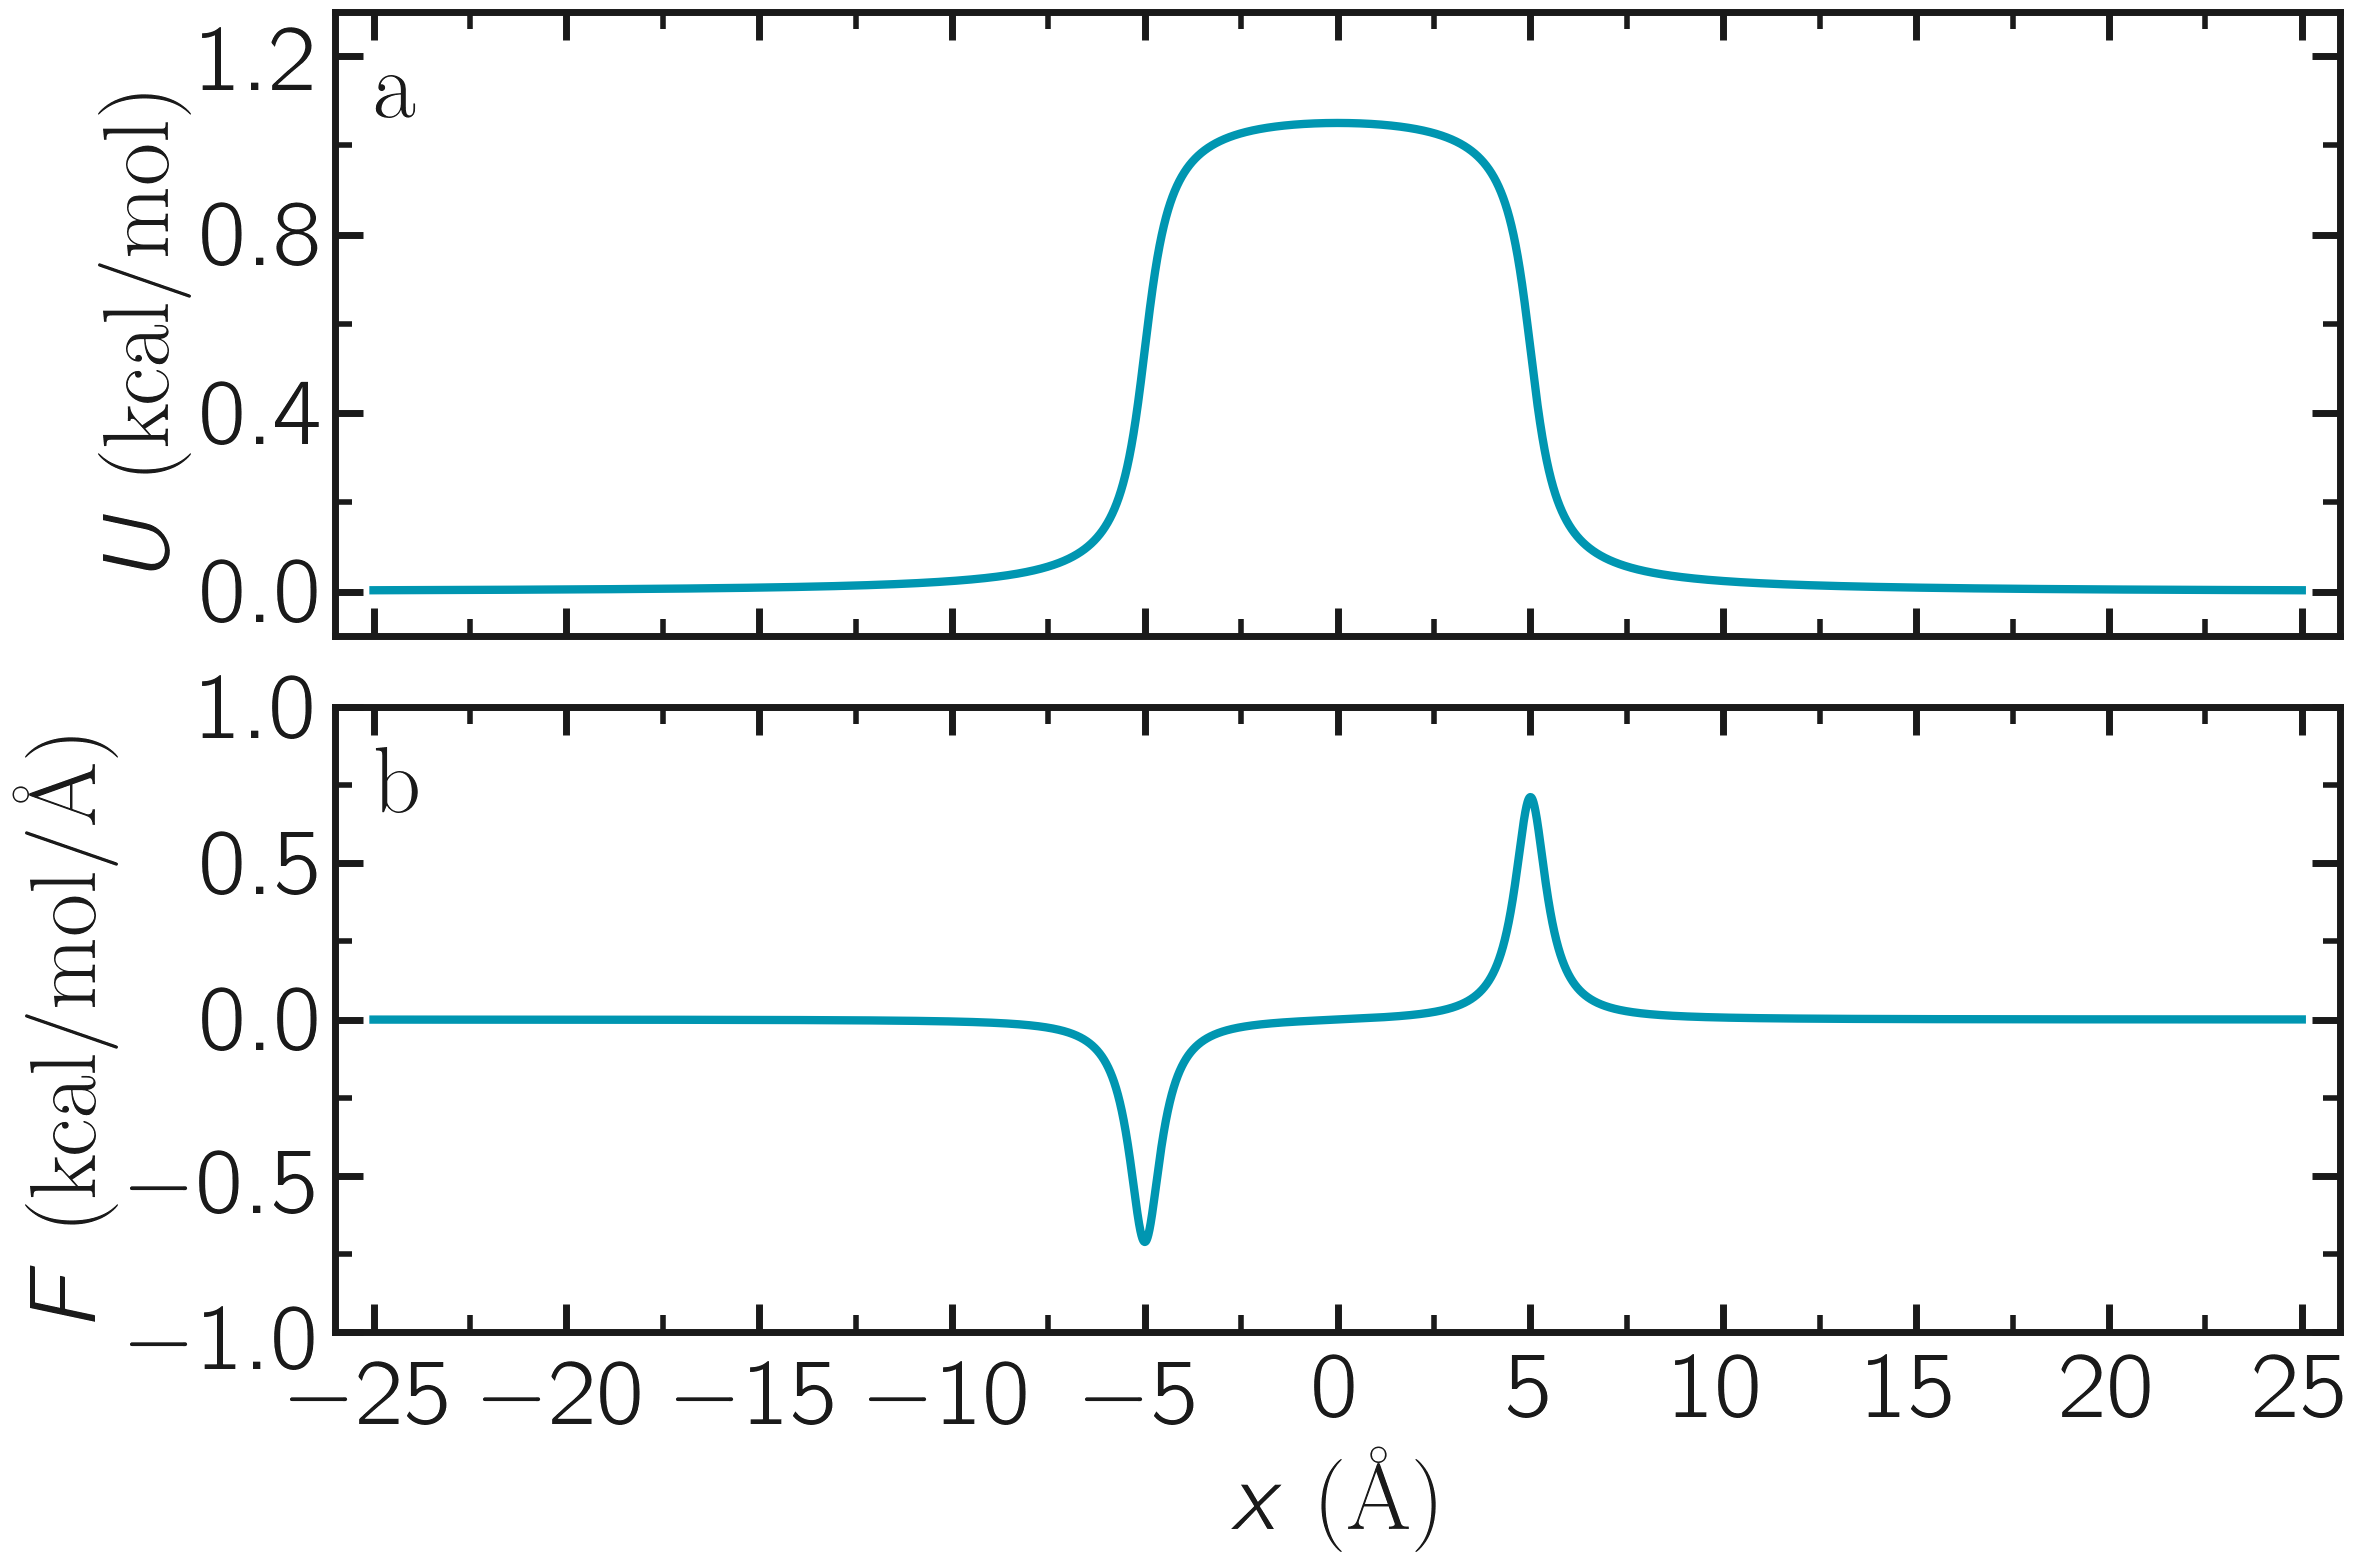
\includegraphics[width=\linewidth]{US-potential}
\caption{Potential $U$ given in Eq.~\eqref{eq:U} (a) and force $F$ given in
Eq.~\eqref{eq:F} (b) as functions of the coordinate $x$. Here,
$U_0 = 0.36~\text{kcal/mol}$, $\delta = 1.0~\text{\AA{}}$, and $x_0 = 10~\text{\AA{}}$.}
\label{fig:potential}
\end{figure}

We impose the force $F(x)$ to the atoms in the simulation
using the \lmpcmd{fix addforce} command.  Add the following
lines to \flecmd{free-energy.lmp}:
% SG: apparently variable can't be cutted in 2 lines, either warn the reader, or find
% a way to write these commands on the entire width of the page, or divide the variables
% into several variables
\begin{lstlisting}
variable U atom ${U0}*atan((x+${x0})/${dlt})&
    -${U0}*atan((x-${x0})/${dlt})
variable F atom ${U0}/((x-${x0})^2/${dlt}^2+1)/${dlt}&
    -${U0}/((x+${x0})^2/${dlt}^2+1)/${dlt}
fix myadf all addforce v_F 0.0 0.0 energy v_U
\end{lstlisting}
Next, we combine the \lmpcmd{fix nve} with a \lmpcmd{fix langevin} thermostat:
\begin{lstlisting}
fix mynve all nve
fix mylgv all langevin 119.8 119.8 500 30917
\end{lstlisting}
When combining these two commands, the MD simulation operates
in the NVT ensemble, maintaining a constant number of
atoms $N$, constant volume $V$, and a temperature $T$ that
fluctuates around a target value.
% SG: may be discuss the choice of constant "500" -> chosen for a relatiely weak coupling with thermostat (add a box?)

To ensure that the equilibration time is sufficient, we will track the evolution of
the number of atoms in the central - energetically unfavorable - region,
referred to as \lmpcmd{mymes}, using the \lmpcmd{n\_center} variable:
\begin{lstlisting}
region mymes block -${x0} ${x0} INF INF INF INF
variable n_center equal count(all,mymes)
thermo_style custom step temp etotal v_n_center
thermo 10000

dump viz all image 50000 myimage-*.ppm type type &
    shiny 0.1 box yes 0.01 view 180 90 zoom 6 &
    size 1600 500 fsaa yes
dump_modify viz backcolor white acolor 1 cyan &
    adiam 1 3 boxcolor black
\end{lstlisting}
A \lmpcmd{dump image} command was also added for system visualization.

Finally, let us perform an equilibration of 50000 steps,
using a timestep of $2\,\text{fs}$, corresponding to a total duration of $100\,\text{ps}$:
\begin{lstlisting}
timestep 2.0
run 50000
\end{lstlisting}
Run the simulation with LAMMPS.  The number of atoms in the
central region, $n_\mathrm{center}$, reaches its equilibrium value after approximately $40\,\text{ps}$
(Fig.~\ref{fig:US-density-evolution}).  A snapshot of the equilibrated system is shown in Fig.~\ref{fig:US-system-unbiased}.

\paragraph{Run and data acquisition}

Once the system is equilibrated, we will record the density profile of
the atoms along the $x$-axis using the \lmpcmd{ave/chunk} command.
Add the following line to \flecmd{free-energy.lmp}:
\begin{lstlisting}
reset_timestep 0

thermo 200000

compute cc1 all chunk/atom bin/1d x 0.0 2.0
fix myac all ave/chunk 100 20000 2000000 &
    cc1 density/number file free-sampling.dat

run 2000000
\end{lstlisting}
The step count is reset to 0 using \lmpcmd{reset\_timestep} to synchronize it
with the output times of \lmpcmd{fix density/number}.  Run the simulation using
LAMMPS.

\begin{figure}
\centering
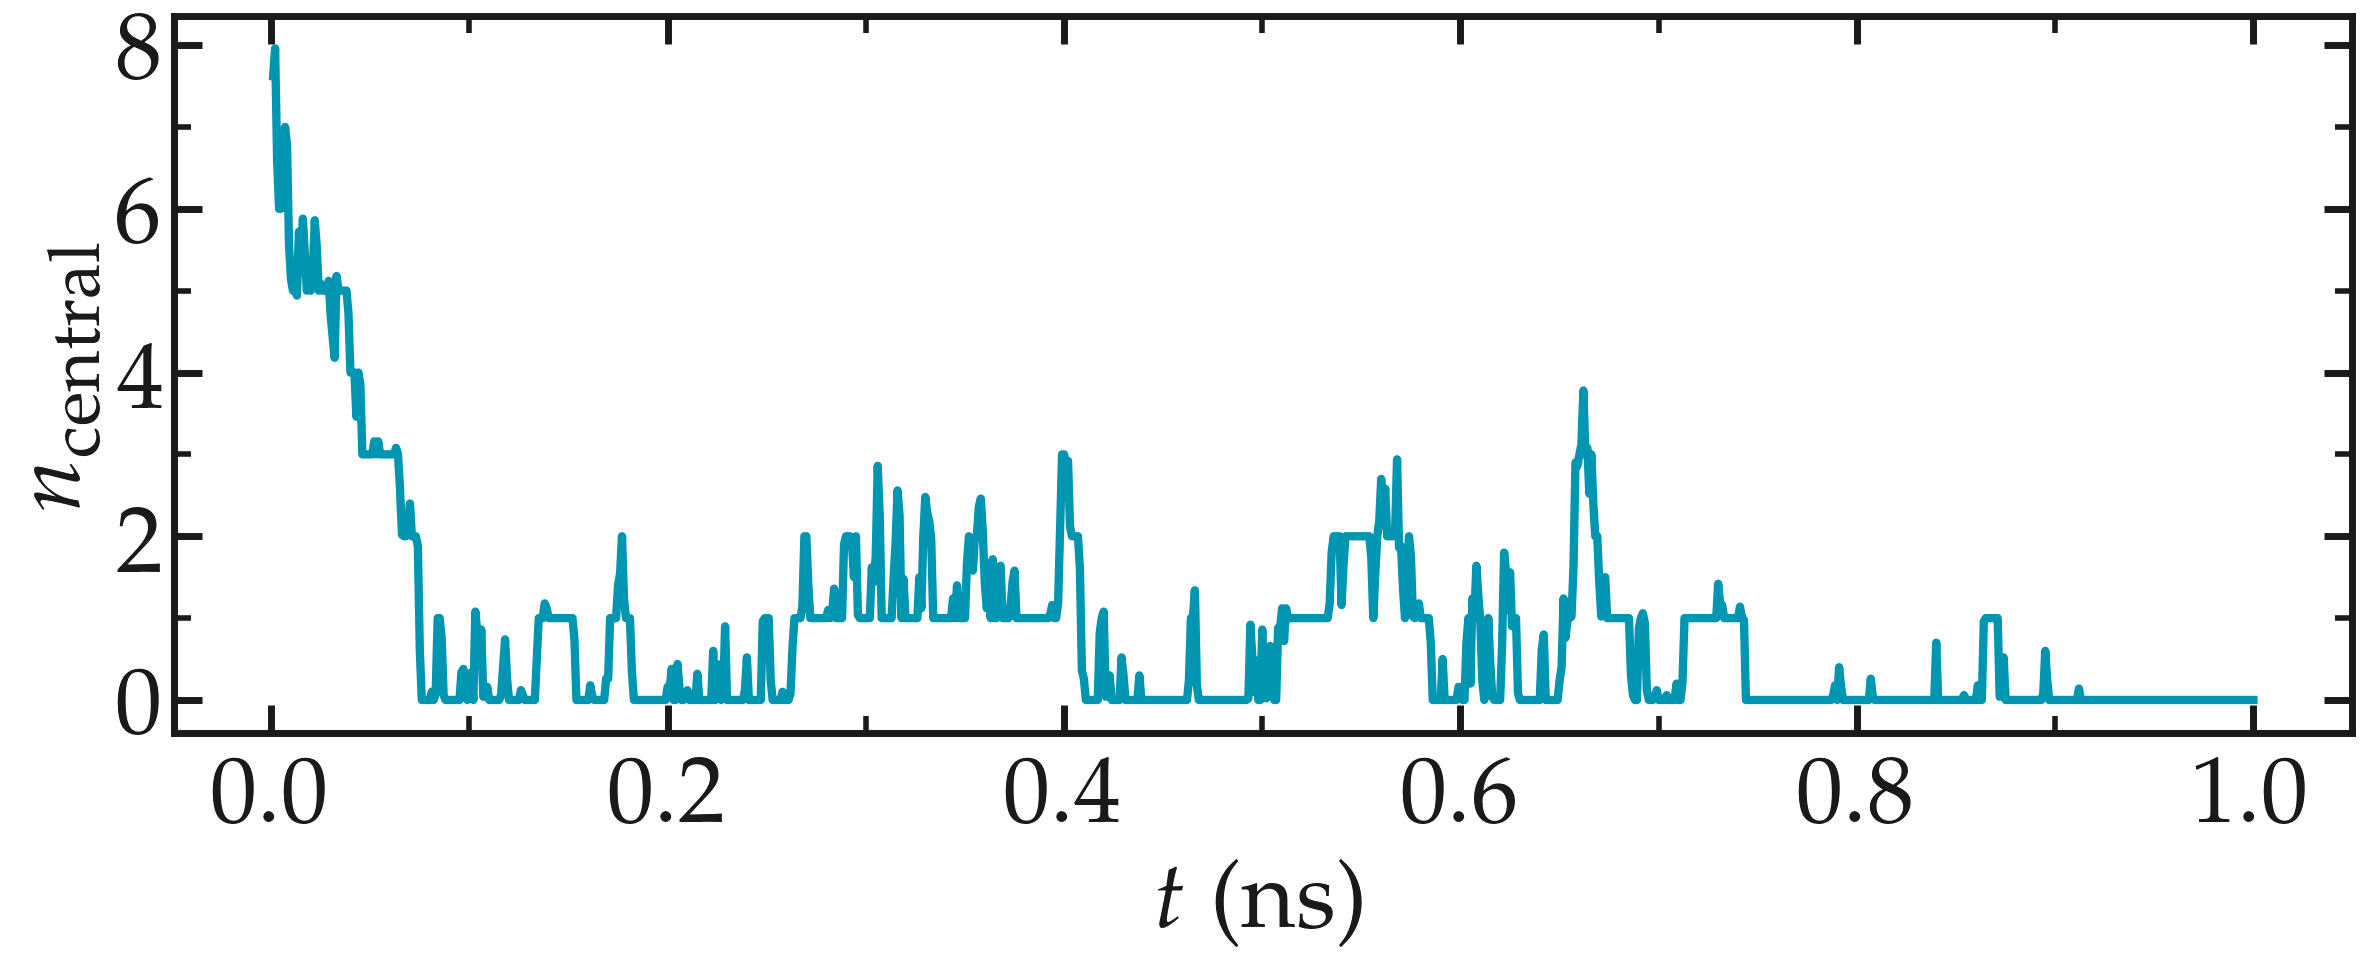
\includegraphics[width=\linewidth]{US-density-evolution}
\caption{Evolution of the number of atoms $n_\text{center}$ in the central
region \lmpcmd{mymes} as a function of time $t$ during equilibration.  The dark line
is $n_\text{center} = 22 \exp(-t/160)+5$ and serves as a guide for the eyes.
Here, $U_0 = 0.36~\text{kcal/mol}$, $\delta = 1.0~\text{\AA{}}$, and $x_0 = 10~\text{\AA{}}$.}
\label{fig:US-density-evolution}
\end{figure}

\paragraph{Data analysis}

Once the simulation is complete, the density profile from \flecmd{free-sampling.dat}
shows that the density in the center of the box is
about two orders of magnitude lower than inside the reservoir (Fig.~\ref{fig:US-density}\,a).
Next, we plot $-R T \ln(\rho/\rho_\mathrm{bulk})$ (i.e.~Eq.~\eqref{eq:G} where
the pressure ratio $p/p_\mathrm{bulk}$ is replaced by the density ratio
$\rho/\rho_\mathrm{bulk}$, assuming the system behaves as an ideal gas) and compare it
with the imposed potential $U$ from Eq.~\eqref{eq:U} (Fig.~\ref{fig:US-density}\,b).
The reference density, $\rho_\text{bulk} = 0.0009~\text{\AA{}}^{-3}$,
was estimated by measuring the density of the reservoir from the raw density
profiles.  The agreement between the MD results and the imposed energy profile
is excellent, despite some noise in the central part, where fewer data points
are available due to the repulsive potential.

\begin{figure}
\centering
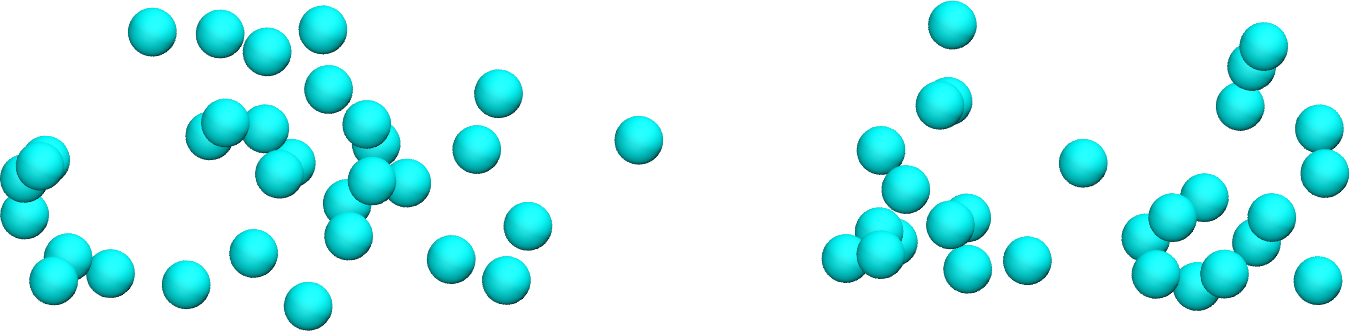
\includegraphics[width=\linewidth]{US-system-unbiased}
\caption{Snapshot of the system simulated during the free sampling
step of \hyperref[umbrella-sampling-label]{Tutorial 7}.
The atoms density is the lowest in the central
part of the box, \lmpcmd{mymes}.  Here,
$U_0 = 0.36~\text{kcal/mol}$, $\delta = 1.0~\text{\AA{}}$, and $x_0 = 10~\text{\AA{}}$.}
\label{fig:US-system-unbiased}
\end{figure}

\begin{figure}
\centering
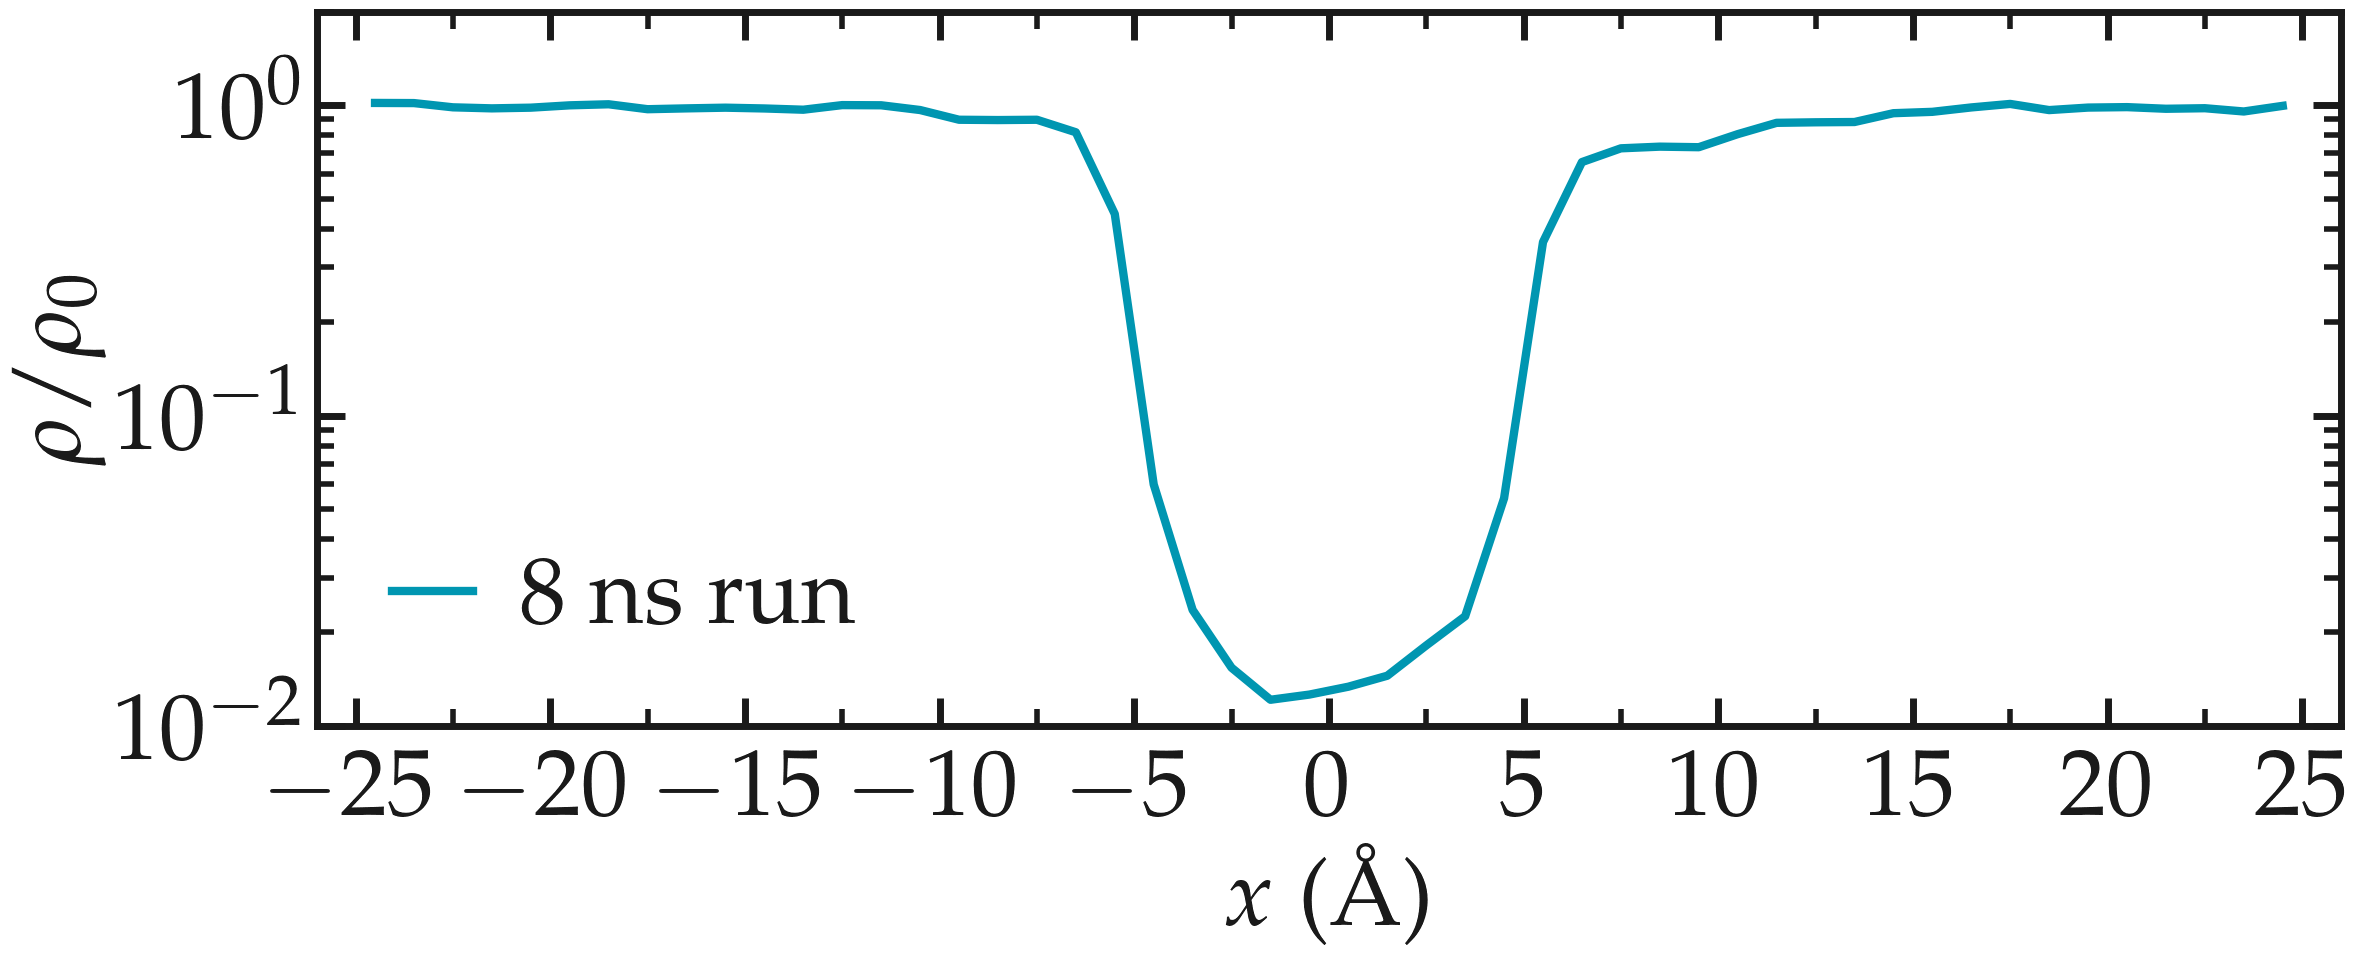
\includegraphics[width=\linewidth]{US-density}
\caption{a) Fluid density $\rho$ along the $x$ direction.
b) Potential $U$ as a function of $x$ measured using free sampling (blue disks)
compared to the imposed potential given in Eq.~\eqref{eq:U} (dark line).
Here, $U_0 = 0.36~\text{kcal/mol}$, $\delta = 1.0~\text{\AA{}}$, $x_0 = 10~\text{\AA{}}$,
and the measured reference density in the reservoir is $\rho_\text{bulk} = 0.0009~\text{\AA{}}^{-3}$.} % SG: check units of rho bulk
\label{fig:US-density}
\end{figure}

\paragraph{The limits of free sampling}

Increasing the value of $U_0$ reduces the average number of atoms in the central
region, making it difficult to achieve a high-resolution free energy profile.
For example, running the same simulation with $U_0 = 10 \epsilon$,
corresponding to $U_0 \approx 10 k_\text{B} T$, results in no atoms exploring
the central part of the simulation box during the simulation.
In such a case, employing an enhanced sampling method is recommended, as done in the next section.

\subsubsection{Method 2: Umbrella sampling}

Umbrella sampling is a biased molecular dynamics method in which additional forces
are added to a chosen atom to force it to explore the more unfavorable areas of
the system~\cite{kastner2011umbrella, allen2017computer, frenkel2023understanding}.
Here, to encourage one of the atoms to explore the central region of the box,
we apply a potential $V$ and force it to move along the $x$-axis. The chosen path
is called the axis of reaction. Several simulations (called windows) will be
conducted with varying positions for the center of the applied biasing. The results
will be analyzed using the weighted histogram analysis method (WHAM)~\cite{kumar1992weighted},
which allows for the removal of the biasing effect and ultimately deduces the
unbiased free energy profile.

\paragraph{LAMMPS input script}

Open the file named \flecmd{umbrella-sampling.lmp}, which should
contain the following lines:
\begin{lstlisting}
variable sigma equal 3.405
variable epsilon equal 0.238
variable U0 equal 10*${epsilon}
variable dlt equal 1.0
variable x0 equal 10
variable k equal 0.5

units real
atom_style atomic
pair_style lj/cut 3.822
pair_modify shift yes
boundary p p p
\end{lstlisting}
The first difference from the previous case is the larger value
for the repulsive potential $U_0$, which makes the central area
of the system very unlikely to be visited by free particles.  The second
difference is the introduction of the variable $k$, which will be used for
the biasing potential.

Let us create a simulation box with two atom types, including a single particle of type 2,
by adding the following lines to \flecmd{umbrella-sampling.lmp}:
\begin{lstlisting}
region myreg block -50 50 -15 15 -50 50
create_box 2 myreg
create_atoms 2 single 0 0 0
create_atoms 1 random 199 34134 myreg overlap 3 maxtry 50
\end{lstlisting}
Next, we assign the same mass and LJ parameters to both atom types
1 and 2, and place the atoms of type 2 into a group named \lmpcmd{topull}:
\begin{lstlisting}
mass * 39.948
pair_coeff * * ${epsilon} ${sigma}
group topull type 2
\end{lstlisting}
Then, the same potential $U$ and force $F$ are applied to all the atoms,
together with the same \lmpcmd{fix nve} and \lmpcmd{fix langevin} commands:
\begin{lstlisting}
variable U atom ${U0}*atan((x+${x0})/${dlt})&
    -${U0}*atan((x-${x0})/${dlt})
variable F atom ${U0}/((x-${x0})^2/${dlt}^2+1)/${dlt}&
    -${U0}/((x+${x0})^2/${dlt}^2+1)/${dlt}
fix myadf all addforce v_F 0.0 0.0 energy v_U

fix mynve all nve
fix mylgv all langevin 119.8 119.8 500 30917
\end{lstlisting}
Next, we perform a brief equilibration to prepare for the
umbrella sampling run:
\begin{lstlisting}
thermo 5000

dump viz all image 50000 myimage-*.ppm type type &
    shiny 0.1 box yes 0.01 view 180 90 zoom 6 &
    size 1600 500 fsaa yes
dump_modify viz backcolor white acolor 1 cyan &
acolor 2 red adiam 1 3 adiam 2 3 boxcolor black

timestep 2.0
run 50000
\end{lstlisting}

So far, our code resembles that of Method 1, except for the additional particle
of type 2.  Particles of types 1 and 2 are identical, with the same mass
and LJ parameters.  However, the particle of type 2 will also
be exposed to the biasing potential $V$, which forces it to explore the
central part of the box (Fig.~\ref{fig:US-system-biased}).

\begin{figure}
\centering
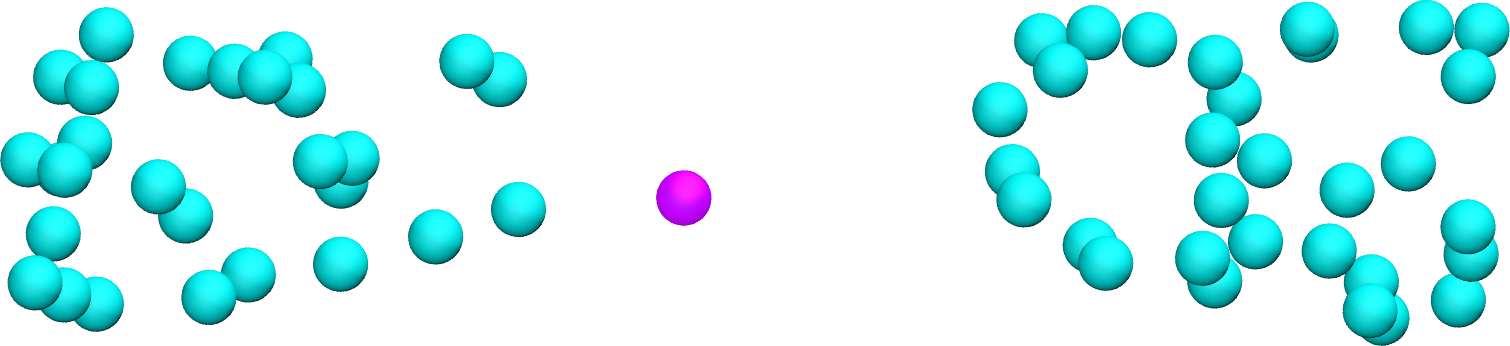
\includegraphics[width=\linewidth]{US-system-biased}
\caption{Snapshot of the system simulated during the umbrella sampling
step of \hyperref[umbrella-sampling-label]{Tutorial 7}, showing type-1 atoms
in cyan and the type-2 atom in red.  Only the type-2 atom explores the central part of the box,
\lmpcmd{mymes}, due to the additional biasing potential $V$. Parmaeters are
$U_0 = 2.38~\text{kcal/mol}$, $\delta = 1.0~\text{\AA{}}$, and $x_0 = 10~\text{\AA{}}$.}
\label{fig:US-system-biased}
\end{figure}

Now, we create a loop with 15 steps and progressively move the center of the
bias potential by increments of 0.4\,nm.  Add the following lines to \flecmd{umbrella-sampling.lmp}:
\begin{lstlisting}
variable a loop 25
label loop

variable xdes equal 4*${a}-32
variable xave equal xcm(topull,x)
fix mytth topull spring tether ${k} ${xdes} 0 0 0

run 20000

fix myat1 all ave/time 10 10 100 &
    v_xave v_xdes file umbrella-sampling.${a}.dat

run 200000
unfix myat1
next a
jump SELF loop
\end{lstlisting}
The \lmpcmd{spring} command imposes the additional harmonic potential $V$ with
the previously defined spring constant $k$.  The center of the harmonic
potential, $x_\text{des}$, successively takes values
from $-28\,\text{\AA}$ to $28\,\text{\AA}$.  For each value of $x_\text{des}$,
an equilibration step of 40\,ps is performed, followed by a step
of 400\,ps during which the position of the particle of
type 2 along the $x$-axis, $x_\text{ave}$, is saved in data files named \flecmd{umbrella-sampling.i.dat},
where $i$ ranges from 1 to 15.  Run the \flecmd{umbrella-sampling.lmp} file using LAMMPS.

\begin{note}
The value of $k$ should be chosen with care:
if $k$ is too small the particle won't follow the biasing potential,
and if $k$ is too large there will be no overlapping between
the different windows, leading to poor reconstruction of the free energy profile.
\end{note}

\paragraph{WHAM algorithm}

To generate the free energy profile from the particle positions
saved in the \flecmd{umbrella-sampling.i.dat} files,
we use the WHAM algorithm as implemented by Marc Grossfield~\cite{grossfieldimplementation}.
You can download it from \href{http://membrane.urmc.rochester.edu/?page_id=126}{Alan Grossfield}'s
website.  The executable called \flecmd{wham} generated by following the instructions
from the website must be placed next to \flecmd{umbrella-sampling.lmp}.  To apply
the WHAM algorithm to our simulation, we need a metadata file containing:
\begin{itemize}
\item the paths to all the data files,
\item the values of $x_\text{des}$,
\item the values of $k$.
\end{itemize}
Download the \href{\filepath tutorial7/umbrella-sampling.meta}{\dwlcmd{umbrella-sampling.meta}} file
and save it next to \flecmd{umbrella-sampling.lmp}.  Then, run the WHAM algorithm
by typing the following command in the terminal:
\begin{lstlisting}
./wham -30 30 50 1e-8 119.8 0 \
    umbrella-sampling.meta umbrella-sampling.dat
\end{lstlisting}
where -30 and 30 are the boundaries, 50 is the number of bins, 1e-8 is the tolerance,
and 119.8 is the temperature in Kelvin.  A file called \flecmd{umbrella-sampling.dat} is created,
containing the free energy profile in kcal/mol.  The resulting PMF can be compared
with the imposed potential $U$, showing excellent agreement
(Fig.~\ref{fig:US-freenergy}).  Remarkably, this excellent agreement is achieved despite
the very short calculation time and the high value for the energy barrier.
Achieving similar results through free sampling would require performing extremely
long and computationally expensive simulations.

\begin{figure}
\centering
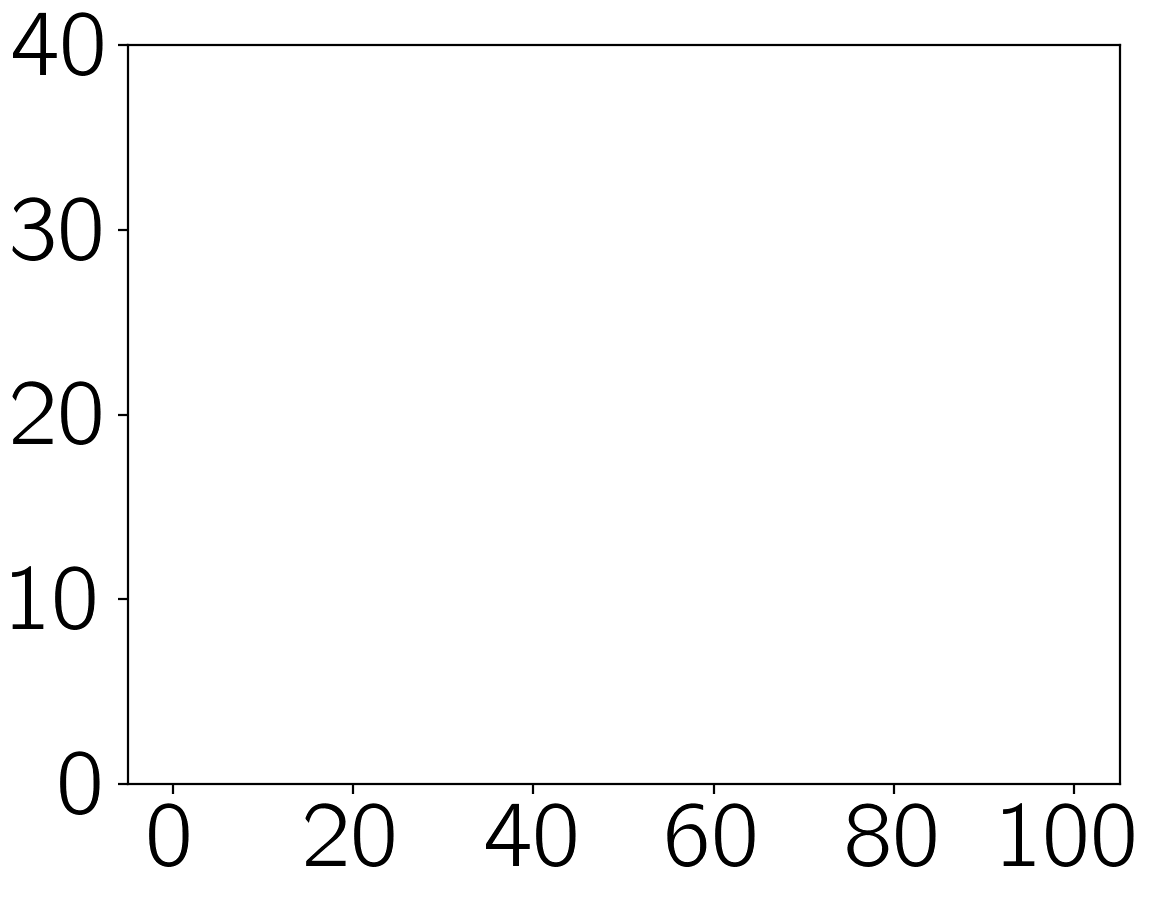
\includegraphics[width=\linewidth]{US-free-energy}
\caption{The potential $U$ as a function of $x$, measured using umbrella
sampling during \hyperref[umbrella-sampling-label]{Tutorial 7} (blue disks),
is compared to the imposed potential given in Eq.~\eqref{eq:U}
(dark line).  Parameters are $U_0 = 2.38~\text{kcal/mol}$, $\delta = 1.0~\text{\AA{}}$,
and $x_0 = 10~\text{\AA{}}$.}
\label{fig:US-freenergy}
\end{figure}

\subsection{Tutorial 8: Reactive Molecular Dynamics}
\label{bond-react-label}

The goal of this tutorial is to create a model of a carbon nanotube (CNT) embedded
in a polymer melt made of polystyrene (PS) (Fig.~\ref{fig:REACT}).  The
REACTER protocol is used to simulate the polymerization of styrene monomers, and the
polymerization reaction is followed in time \cite{gissinger2017polymer, gissinger2020reacter, gissinger2024molecular}.
In contrast with AIREBO (\hyperref[carbon-nanotube-label]{Tutorial 2})
and ReaxFF (\hyperref[reactive-silicon-dioxide-label]{Tutorial 5}), the REACTER
protocol relies on the use of a \textit{classical} force field.

\begin{figure}
\centering
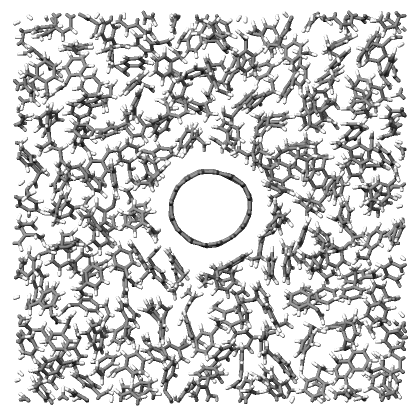
\includegraphics[width=\linewidth]{REACT.png}
\caption{Initial configuration for \hyperref[bond-react-label]{Tutorial 8}.
The system consists of 200 styrene molecules packed around a single-walled
CNT, with a mass density for the whole system of $0.9~\text{g/cm}^3$.}
\label{fig:REACT}
\end{figure}

\subsubsection{Creating the system}

To begin this tutorial, select \guicmd{Start Tutorial 8} from the
\guicmd{Tutorials} menu of \lammpsgui{} and follow the instructions.
The editor should display the following content corresponding to \flecmd{mixing.lmp}:
\begin{lstlisting}
units real
boundary p p p
atom_style full

kspace_style pppm 1.0e-5
pair_style lj/class2/coul/long 8.5
angle_style class2
bond_style class2
dihedral_style class2
improper_style class2

pair_modify tail yes mix sixthpower
special_bonds lj/coul 0 0 1
\end{lstlisting}
The \lmpcmd{class2} styles compute a 6/9 Lennard-Jones potential~\cite{sun1998compass}.
The \textit{class2} bond, angle, dihedral, and improper styles are used as
well, see the documentation for a description of their respective potentials.
The \lmpcmd{mix sixthpower} imposes the following mixing rule for the calculation
of the cross coefficients:
\begin{eqnarray}
\nonumber
\sigma_{ij} & = & 2^{-1/6} (\sigma^6_i+\sigma_j^6)^{1/6}, ~ \text{and} \\
\nonumber
\epsilon_{ij} & = & \dfrac{2 \sqrt{\epsilon_i \epsilon_j} \sigma^3_i \sigma^3_j}{\sigma^6_i+\sigma_j^6}.
\end{eqnarray}

Let us read the \href{\filepath tutorial8/CNT.data}{\dwlcmd{CNT.data}} file, which
contains a periodic single-walled CNT.  Add the following line to \flecmd{mixing.lmp}:
\begin{lstlisting}
read_data CNT.data extra/special/per/atom 20
\end{lstlisting}
The CNT is approximately $1.1~\text{nm}$ in diameter and $1.6\,\text{nm}$ in length, oriented
along the $x$-axis. The simulation box is as large as 5.2~nm in the two other dimensions,
making it straightforward to fill the box with styrene.
To add 200 styrene molecules to the simulation box, using the
\href{\filepath tutorial8/styrene.mol}{\dwlcmd{styrene.mol}} file.
Include the following commands to \flecmd{mixing.lmp}:
\begin{lstlisting}
molecule styrene styrene.mol
create_atoms 0 random 200 8305 NULL overlap 2.75 &
    maxtry 500 mol styrene 7687
\end{lstlisting}
Finally, let us use the \lmpcmd{minimize} command to reduce the potential energy of the system:
\begin{lstlisting}
minimize 1.0e-4 1.0e-6 100 1000
reset_timestep 0
\end{lstlisting}

Then, let us densify the system to a target value of $0.9~\text{g/cm}^3$
by manually shrinking the simulation box at a constant rate.  The dimension parallel
to the CNT axis is maintained fixed because the CNT is periodic in that direction.
Add the following commands to \flecmd{mixing.lmp}:
% SG: I removed the loop local, unless its important? But if it is, we have to
% explain what it does and why it was chosen here.
\begin{lstlisting}
velocity all create 530 9845 dist gaussian rot yes
fix mynvt all nvt temp 530 530 100

fix mydef all deform 1 y erate -0.0001 z erate -0.0001
variable rho equal density
fix myhal all halt 10 v_rho > 0.9 error continue

thermo 200
thermo_style custom step temp pe etotal press density

run 9000
\end{lstlisting}
The \lmpcmd{fix halt} command is used to stop the box shrinkage once the
target density is reached.

For the next stage of the simulation, we will use \lmpcmd{dump image} to
output images every 200 steps:
\begin{lstlisting}
dump viz all image 200 myimage-*.ppm &
  type type shiny 0.1 box no 0.01 size 1000 1000 &
  view 90 0 zoom 1.8 fsaa yes bond atom 0.5
dump_modify viz backcolor white &
  acolor cp gray acolor c=1 gray &
  acolor c= gray acolor c1 deeppink &
  acolor c2 deeppink acolor c3 deeppink &
  adiam cp 0.3 adiam c=1 0.3 &
  adiam c= 0.3 adiam c1 0.3 &
  adiam c2 0.3 adiam c3 0.3 &
  acolor hc white adiam hc 0.15
\end{lstlisting}
For the following $10~\text{ps}$, let us equilibrate the densified system
in the constant-volume ensemble, and write the final state of the
system in a file named \flecmd{mixing.data}:
\begin{lstlisting}
unfix mydef
unfix myhal
reset_timestep 0

group CNT molecule 1
fix myrec CNT recenter NULL 0 0 units box shift all

run 10000

write_data mixing.data
\end{lstlisting}
For visualization purposes, the atoms from the CNT \lmpcmd{group} is moved
to the center of the box using \lmpcmd{fix recenter}.
As the time progresses, the system density,
$\rho$, gradually converges toward the target value of $0.8$\,g/cm$^3$ (Fig.~\ref{fig:evolution-density}\,a).
Meanwhile, the total energy of the system initially evolves rapidly, reflecting the
densification process, and then eventually stabilizes (Fig.~\ref{fig:evolution-density}\,b).
The final state is shown in Fig.~\ref{fig:REACT}.

\begin{figure}
\centering
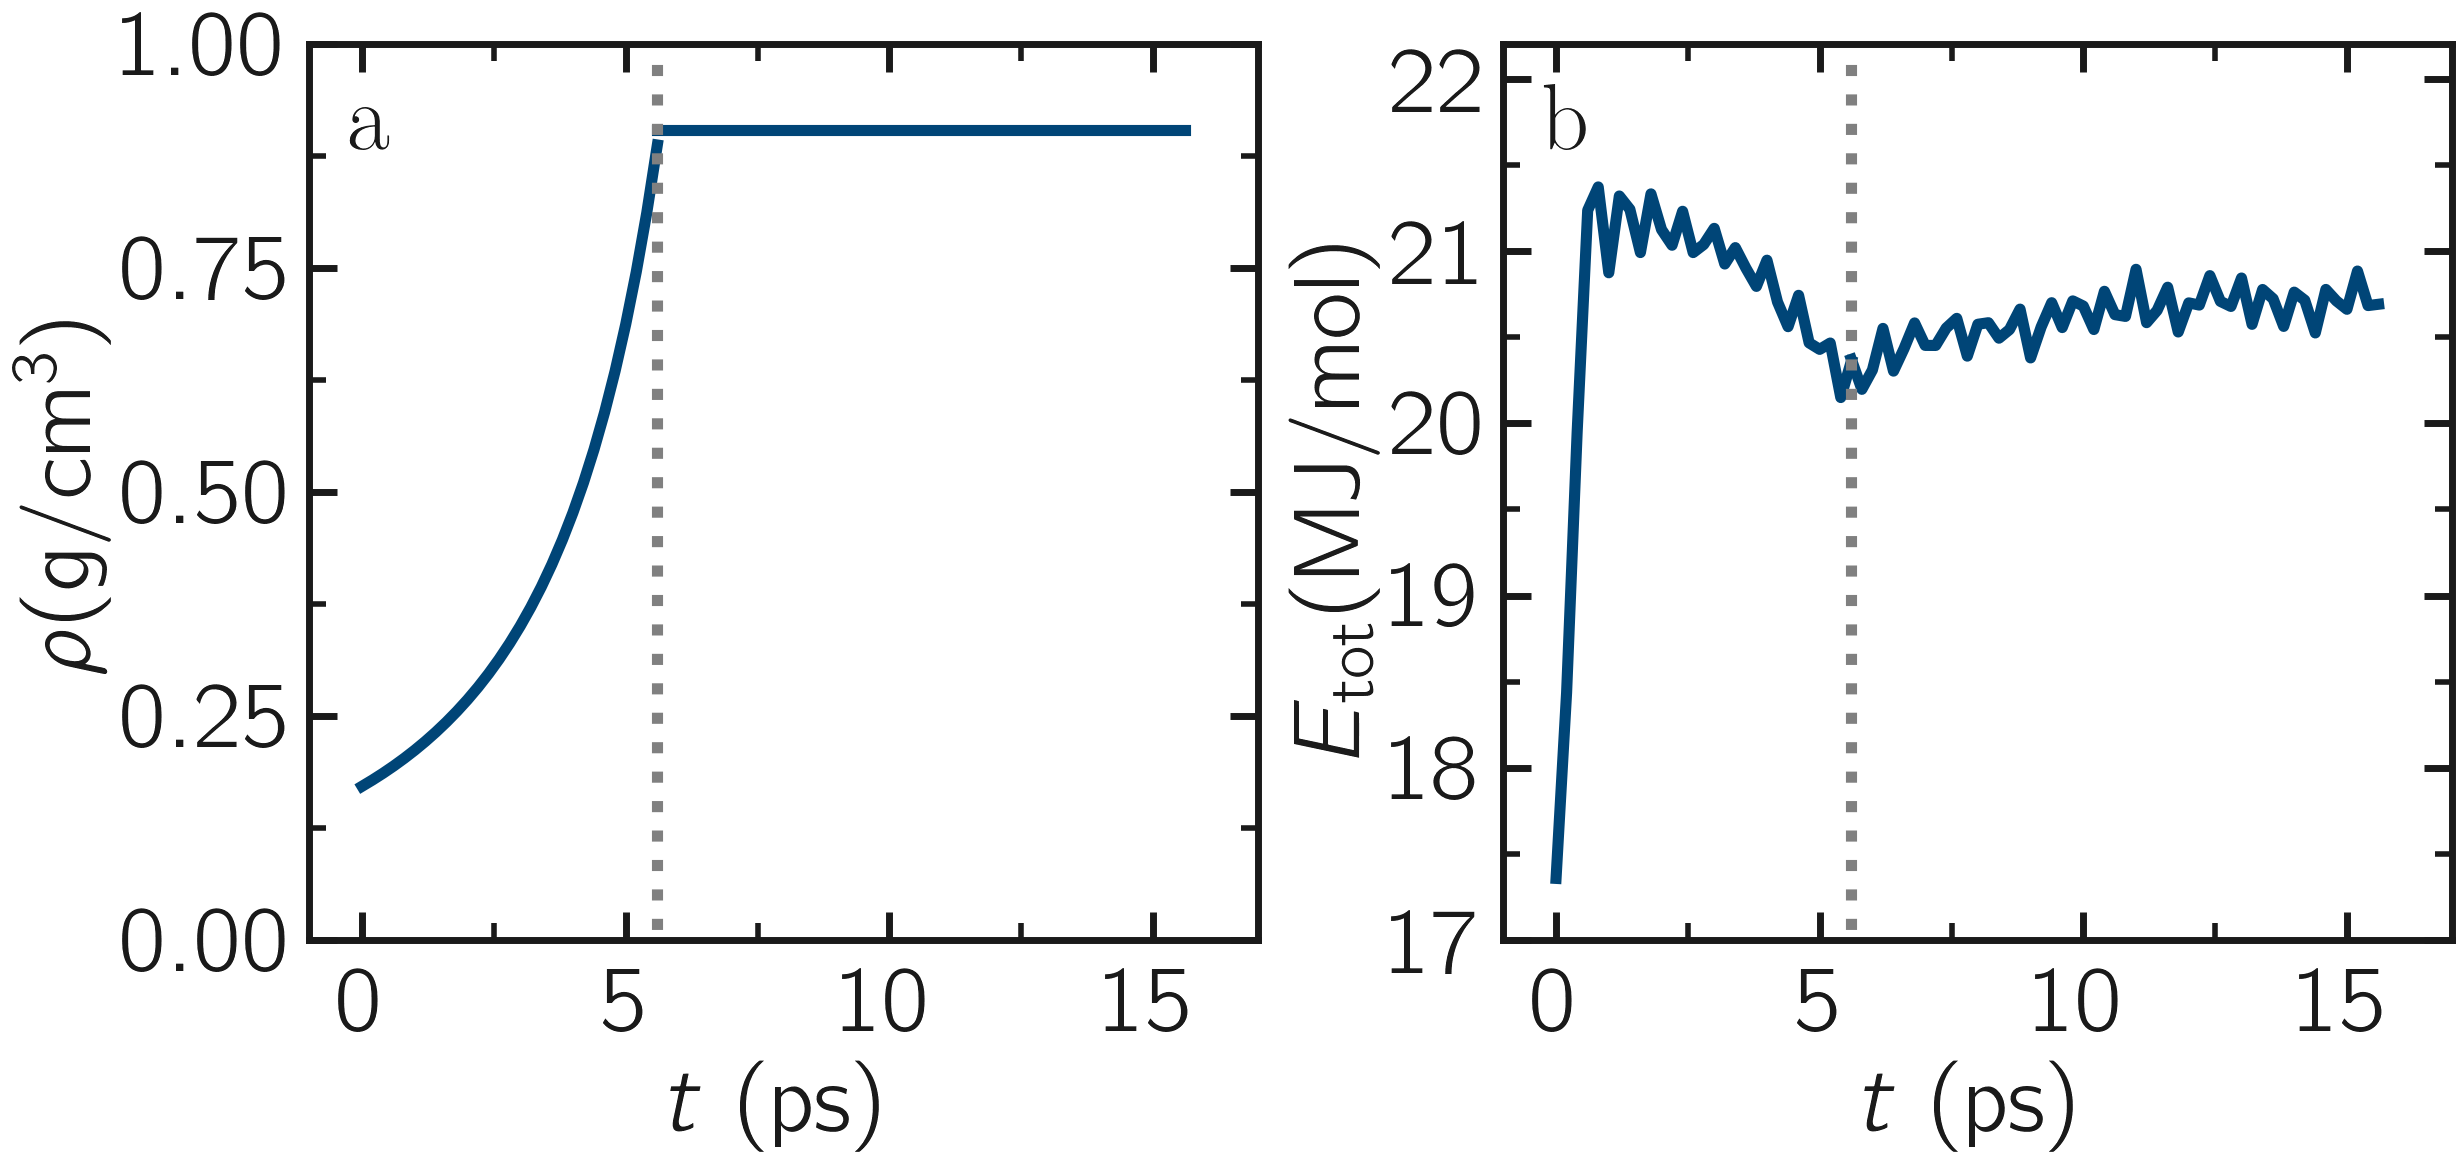
\includegraphics[width=\linewidth]{REACT-mixing}
\caption{a) Evolution of the density, $\rho$, as a function of the
time, $t$, during equilibration of the system from \hyperref[bond-react-label]{Tutorial 8}.
b) Evolution of the total energy, $E_\text{tot}$, of the system.
The vertical dashed lines mark the transition between the different
phases of the simulation.}
\label{fig:evolution-density}
\end{figure}

\subsubsection{Reaction templates}

The REACTER protocol enables the modeling of chemical reactions using
classical force fields.  The user must provide a molecule template for the reactants,
a molecule template for the products, and a \flecmd{reaction map} file that
provides an atom mapping between the two templates.  The reaction map file also includes
additional information, such as which atoms act as initiators for the reaction and which
serve as edge atoms to connect the rest of a long polymer chain in the simulation.

There are three reactions to define: (1) the polymerization of two styrene monomers,
(2) the addition of a styrene monomer to the end of a growing polymer chain, and (3) the
linking of two polymer chains.  Download the three files associated with each reaction.
The first reaction uses the prefix `M-M' for the pre-reaction template,
post-reaction template, and reaction map file:
\begin{itemize}
\item \href{\filepath tutorial8/M-M_pre.mol}{\dwlcmd{M-M$\_$pre.mol}},
\item \href{\filepath tutorial8/M-M_post.mol}{\dwlcmd{M-M$\_$post.mol}},
\item \href{\filepath tutorial8/M-M.rxnmap}{\dwlcmd{M-M.rxnmap}}.
\end{itemize}
The second reaction uses the prefix `M-P',
\begin{itemize}
\item \href{\filepath tutorial8/M-P_pre.lmpmol}{\dwlcmd{M-P$\_$pre.mol}},
\item \href{\filepath tutorial8/M-P_post.lmpmol}{\dwlcmd{M-P$\_$post.mol}},
\item \href{\filepath tutorial8/M-P.rxnmap}{\dwlcmd{M-P.rxnmap}}.
\end{itemize}
The third reaction uses the prefix `P-P',
\begin{itemize}
\item \href{\filepath tutorial8/P-P_pre.lmpmol}{\dwlcmd{P-P$\_$pre.mol}},
\item \href{\filepath tutorial8/P-P_post.lmpmol}{\dwlcmd{P-P$\_$post.mol}},
\item \href{\filepath tutorial8/P-P.rxnmap}{\dwlcmd{P-P.rxnmap}}.
\end{itemize}
Here, the file names for each reaction use the abbreviation `M' for monomer and `P'
for polymer.

\subsubsection{Simulating the reaction}

The first step, before simulating the reaction, is to import the previously
generated configuration.  Open the file named \flecmd{polymerize.lmp},
which should contain the following lines:
\begin{lstlisting}
units real
boundary p p p
atom_style full

kspace_style pppm 1.0e-5
pair_style lj/class2/coul/long 8.5
angle_style class2
bond_style class2
dihedral_style class2
improper_style class2

pair_modify tail yes mix sixthpower
special_bonds lj/coul 0 0 1

read_data mixing.data &
  extra/bond/per/atom 5  &
  extra/angle/per/atom 15 &
  extra/dihedral/per/atom 15 &
  extra/improper/per/atom 25 &
  extra/special/per/atom 25
\end{lstlisting}
Here, the \lmpcmd{read$\_$data} command is used to import the
previously generated \flecmd{mixing.data} file.  All other commands
have been introduced in earlier parts of the tutorial.

Then, let us import all six molecules templates using the \lmpcmd{molecule} command:
\begin{lstlisting}
molecule mol1 M-M_pre.mol
molecule mol2 M-M_post.mol
molecule mol3 M-P_pre.mol
molecule mol4 M-P_post.mol
molecule mol5 P-P_pre.mol
molecule mol6 P-P_post.mol
\end{lstlisting}
In order to follow the evolution of the reaction with time, let us generate images
of the system using \lmpcmd{dump image}:
\begin{lstlisting}
dump viz all image 200 myimage-*.ppm &
  type type shiny 0.1 box no 0.01 size 1000 1000 &
  view 90 0 zoom 1.8 fsaa yes bond atom 0.5
dump_modify viz backcolor white &
  acolor cp gray acolor c=1 gray &
  acolor c= gray acolor c1 deeppink &
  acolor c2 gray acolor c3 deeppink &
  adiam cp 0.3 adiam c=1 0.3 &
  adiam c= 0.3 adiam c1 0.3 &
  adiam c2 0.3 adiam c3 0.3 &
  acolor hc white adiam hc 0.15
\end{lstlisting}

Let us use \lmpcmd{fix bond/react} by adding the following
line to \flecmd{polymerize.lmp}:
\begin{lstlisting}
fix rxn all bond/react &
  stabilization yes statted_grp 0.03 &
  react R1 all 1 0 3.0 mol1 mol2 M-M.rxnmap &
  react R2 all 1 0 3.0 mol3 mol4 M-P.rxnmap &
  react R3 all 1 0 5.0 mol5 mol6 P-P.rxnmap
\end{lstlisting}
With the \lmpcmd{stabilization} keyword, the \lmpcmd{bond/react} command will
stabilize the atoms involved in the reaction using the \lmpcmd{nve/limit}
command with a maximum displacement of $0.03\,\mathrm{\AA{}}$.  By default,
each reaction is stabilized for 60 time steps.  Each \lmpcmd{react} keyword
corresponds to a reaction, e.g.,~a transformation of \lmpcmd{mol1} into \lmpcmd{mol2}
based on the atom map \lmpcmd{M-M.rxnmap}.  Implementation details about each reaction,
such as the reaction distance cutoffs and the frequency with which to search for
reaction sties, are also specified in this command.

\begin{figure}
\centering
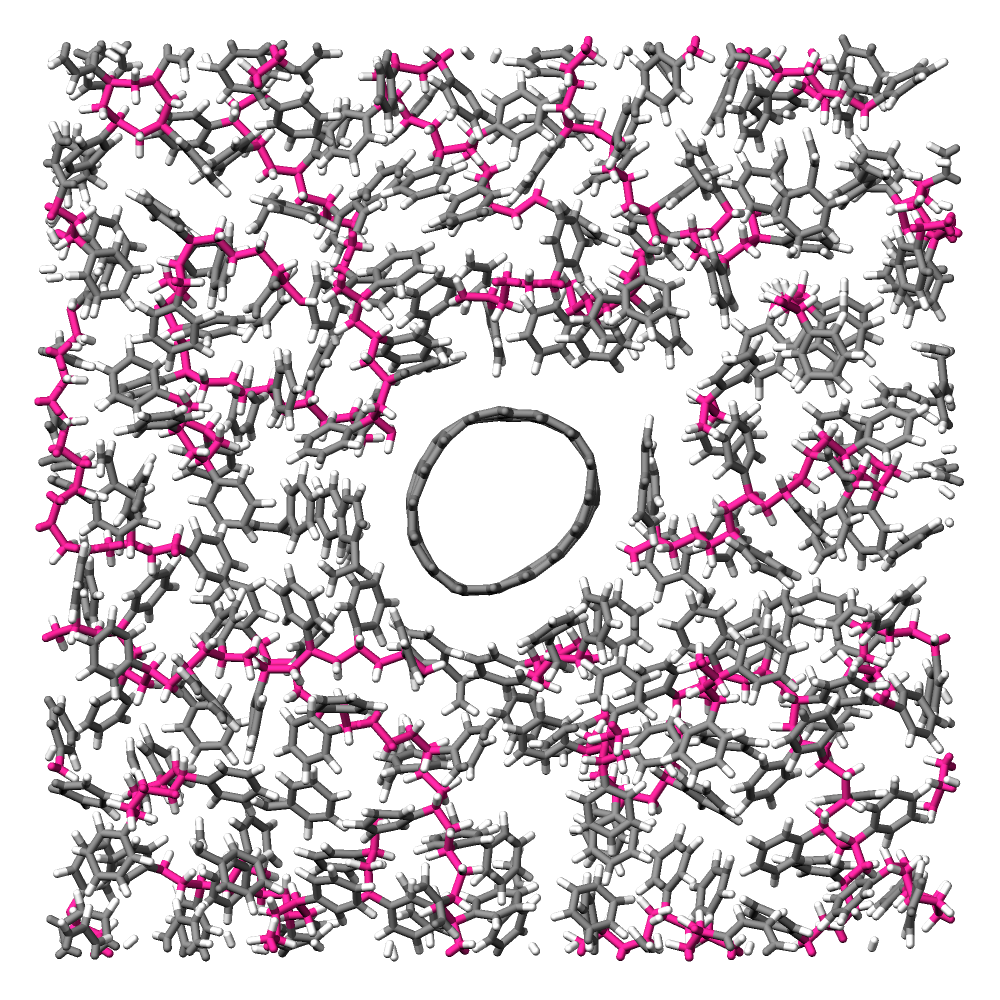
\includegraphics[width=\linewidth]{REACT-final.png}
\caption{Final configuration for \hyperref[bond-react-label]{Tutorial 8}.
The atoms from the formed polymer named \lmpcmd{c1}, \lmpcmd{c2}, and
\lmpcmd{c3} are colored in pink.}
\label{fig:REACT-final}
\end{figure}

\begin{note}
The command \lmpcmd{fix bond/react} creates several groups of atoms that are dynamically updated
to track which atoms are being stabilized and which atoms are undergoing
dynamics with the system-wide time integrator (here, \lmpcmd{fix nvt}).
When reaction stabilization is employed, there should not be a time integrator acting on
the group \mbox{\lmpcmd{all}.}  Instead, the group of atoms not currently
undergoing stabilization is named by appending `\_REACT' to the user-provided prefix.
\end{note}

Add the following commands to \flecmd{polymerize.lmp} to operate in the NVT ensemble
while ensuring that the CNT remains centered in the simulation box:
\begin{lstlisting}
fix mynvt statted_grp_REACT nvt temp 530 530 100
group CNT molecule 1 2 3
fix myrec CNT recenter NULL 0 0 shift all

thermo 1000
thermo_style custom step temp press density f_rxn[*]

run 25000
\end{lstlisting}
Here, the \lmpcmd{thermo custom} command is used
to print the cumulative reaction counts from \lmpcmd{fix rxn}.
Run the simulation using LAMMPS.  As the simulation progresses, polymer chains are
observed forming (Fig.~\ref{fig:REACT-final}).  During this reaction process, the
temperature of the system remains well-controlled (Fig.~\ref{fig:evolution-reacting}\,a),
while the number of reactions, $N_r$, increases with time (Fig.~\ref{fig:evolution-reacting}\,b).

\begin{figure}
\centering
\includegraphics[width=\linewidth]{REACT-reacting}
\caption{a) Evolution of the system temperature, $T$,
as a function of the time, $t$, during the polymerization step of
\hyperref[bond-react-label]{Tutorial 8}.
b) Evolution of the three reaction counts, corresponding respectively to
the polymerization of two styrene monomers (Rxn~1), the  addition of a styrene
monomer to the end of a growing polymer chain (Rxn~2), and to the linking
of two polymer chains (Rxn~3).}
\label{fig:evolution-reacting}
\end{figure}

\section*{Author Contributions}

S.G. conceived and wrote the original online tutorials and underlying Sphinx documentation
for \href{https://lammpstutorials.github.io}{lammpstutorials.github.io}.
J.G. is the principal author of \lmpcmd{fix bond/react} and \lmpcmd{type labels}
support in LAMMPS.  He revised the tutorials to incorporate type labels and wrote Tutorial 8.
A.K. developed the \lammpsgui{} software and assisted in revising the
tutorials for use with it.  All authors participated in the revision and finalization
of the manuscript.

\section*{Potentially Conflicting Interests}

There are no conflicting interests to declare.

\section*{Funding Information}

S.G. acknowledges funding from the European Union's Horizon 2020 research and
innovation programme under the Marie Skłodowska-Curie grant agreement $\text{N}^\circ\;101065060$.
A.K. acknowledges financial support by Sandia National Laboratories under
POs~2149742 and 2407526.

\section*{Author Information}
\makeorcid

\bibliography{journal-article}

%%%%%%%%%%%%%%%%%%%%%%%%%%%%%%%%%%%%%%%%%%%%%%%%%%%%%%%%%%%%
%%% APPENDICES
%%%%%%%%%%%%%%%%%%%%%%%%%%%%%%%%%%%%%%%%%%%%%%%%%%%%%%%%%%%%

\begin{appendices}
\section{Using \lammpsgui{}}
\label{using-lammps-gui-label}

\begin{note}
For simplicity, these tutorials reference keyboard shortcuts
based on the assignments for Linux and Windows.  {macOS} users should
use the ``Command'' key (\cmd) in place of the
``Ctrl'' key when using keyboard shortcuts.
\end{note}

\subsection{Installation}

Precompiled versions of \lammpsgui{} are available for Linux, {macOS},
and Windows on the LAMMPS GitHub Release
page~\cite{lammps_github_release}.  The Linux version is provided in two
formats: as compressed tar archive (.tar.gz) and as a Flatpak
bundle~\cite{flatpak_home}.  The {macOS} version is distributed as a
.dmg installer image, while the Windows version comes as an executable
installer package.

\subsubsection{Installing the Linux .tar.gz Package}

Download the archive (e.g.,~LAMMPS-Linux-x86\_64-GUI-29Aug2024\_update2.tar.gz)
and unpack it.  This will create a folder named LAMMPS\_GUI containing the
included commands, which can be launched directly using ``./lammps-gui'' or
``./lmp'', for example.  Adding this folder to the PATH environment
variable will make these commands accessible from everywhere, without the
need for the ``./'' prefix.

\subsubsection{Installing the Linux Flatpak Bundle}

You have to have Flatpak support installed on Linux machine to be able
to use the Flatpak bundle.  Download the bundle file
(e.g.,~LAMMPS-Linux-x86\_64-GUI-29Aug2024\_update2.flatpak) and then
install it using the following command:
\begin{lstlisting}[language=tcl]
flatpak install --user \
    LAMMPS-Linux-x86_64-GUI-29Aug2024_update2.flatpak
\end{lstlisting}
This will integrate \lammpsgui{} into your desktop environment
(e.g.,~GNOME, KDE, XFCE) where it should appear in the ``Applications''
menu under ``Science''.  Additionally, the ``.lmp'' file extension will be
registered to launch \lammpsgui{} when opening a file with this
extension in the desktop's file manager.

You can also launch \lammpsgui{} from the command-line using the following command:
\begin{lstlisting}[language=tcl]
flatpak run org.lammps.lammps-gui
\end{lstlisting}
Similarly, for launching the LAMMPS command-line executable, use:
\begin{lstlisting}[language=tcl]
flatpak run --command=lmp org.lammps.lammps-gui -in in.lmp
\end{lstlisting}

\subsubsection{Installing the macOS Application Bundle}

After downloading the macOS app bundle image file
(e.g.,~LAMMPS-macOS-multiarch-GUI-29Aug2024\_update2.dmg), double-click
on it.  In the dialog that opens drag the LAMMPS\_GUI app bundle into
the Applications folder.  To enable command-line access, follow the
instructions in the README.txt file.  These macOS app-bundles contain
native executables for both, Intel and Apple CPUs.

After installation, you can launch LAMMPS\_GUI from the Applications
folder.  Additionally, you can drag an input file onto the app or open
files with the ``.lmp'' extension.  Note that the \lammpsgui{} app bundle is
currently not cryptographically signed, so macOS may initially prevent
it from launching.  If this happens, you need to adjust the settings in
the ``Security \& Privacy" system preferences dialog to allow access.

\subsubsection{Installing the Windows package}

Download the \lammpsgui{} installer for Windows
(e.g.,~LAMMPS-Win10-64bit-GUI-29Aug2024\_update2.exe).  Windows may warn
you that the file is from an unknown developer and was downloaded from
the internet.  This happens because neither the installer nor the
\lammpsgui{} application (or any other included applications) have been
cryptographically signed.  You will need to choose to keep the file, and
when launching the installer, confirm that you want to run it despite
the warning.

After installation, a new entry should appear in the Start menu.
Additionally, the ``.lmp'' file extension should be registered with
Windows File Explorer to open \lammpsgui{} when opening a file with the
``.lmp`` extension.  The ``lammps-gui'' and ``lmp'' commands should also
be available in the command-line.

\subsection{Opening, Editing, and Saving Files}

\lammpsgui{} can be launched from the command-line, as explained above, where you
can either launch it without arguments or provide one file name as an argument.  All
other arguments will be ignored.  For example:
\begin{lstlisting}[language=tcl]
lammps-gui input.lmp
\end{lstlisting}
Files can also be opened from the ``File'' menu.  You can select a
file through a dialog and then open it.  Additionally, a history of
the last five opened files is maintained, with entries to open them directly.
Finally, the \texttt{Ctrl-O} keyboard shortcut can also be used to open a file.

When integrated into a desktop environment, it is also possible to open
files with a ``.lmp'' extension or use drag-and-drop.

For the most part, the editor window behaves like other graphical
editors.  You can enter, delete, or copy and paste text.   When entering
text, a pop-up window will appear with possible completions after typing
the first two characters of the first word in a line.  You can
navigate the highlighted options using the up and down arrow keys, and select a
completion by pressing the Enter key or using the mouse.  You can also continue
typing, and the selection in the pop-up will be refined.  For some
commands, there will be completion pop-ups for their
keywords or when a filename is expected, in which case,
the pop-up will list files in the current folder.

As soon as \lammpsgui{} recognizes a command, it applies syntax
highlighting according to built-in categories.  This can help
detect typos, since those may cause \lammpsgui{} not to
recognize the syntax and thus not apply or partially apply
the syntax highlighting.  When you press the \texttt{Tab} key, the line will be
reformatted.  Consistent formatting can improve the readability of
input files, especially long and complex ones.

If the file in the editor has unsaved changes, the word
``\*modified\*'' will appear in the window title.  The current input
buffer can be saved by selecting ``Save'' or ``Save As...'' from the
``File'' menu.  You can also click the ``Save'' icon on the left side
of the status bar, or use the \texttt{Ctrl-S} keyboard shortcut.

\begin{note}
When \lammpsgui{} opens a file, it will \emph{switch} the working directory
to the folder that contains the input file.  The same happens when saving to
a different folder than the current working directory.  The current working
directory can be seen in the status bar at the bottom right.  This is important
to note because LAMMPS input files often require additional files for reading and may
write output files (such as images, trajectory dumps, or averaged data files),
which are typically expected to be in the same folder as the input file.
\end{note}

%The contents of the \textit{Editor} window can be saved by either using
%the ``Save'' or ``Save As'' entry in the ``File'' menu, using the
%\texttt{Ctrl-S} keyboard shortcut or by clicking on the ``Save'' icon
%at the bottom left of the \textit{Editor} window status bar.  For
%running LAMMPS in \lammpsgui{} it is not required to save the buffer.
%The current contents of the buffer will be passed on to LAMMPS.
%However, if you prefer to have your editor buffer automatically saved
%before launching a run or exiting the LAMMPS-GUI, there is a setting for this
%in the \textit{Preferences} dialog.

\subsection{Running LAMMPS}

% mention no log file -> Output window -> Save to file
% SG: the "no log file" is already specified in the "The Output Window" subsection, so may be unecessary?

From within the \lammpsgui{} main window, LAMMPS can be started either from
the \guicmd{Run} menu by selecting the \guicmd{Run LAMMPS from Editor Buffer} entry,
using the keyboard shortcut Ctrl-Enter (Command-Enter on macOS), or by clicking the
green \guicmd{Run} button in the status bar.  While LAMMPS is running, a message on
the left side indicates that LAMMPS is active, along with the number of active threads.
On the right side, a progress bar is displayed, showing the estimated progress
of the current \lmpcmd{run} or \lmpcmd{minimize} command.

\subsection{Creating Snapshot Images}

Open the \guicmd{Image Viewer} using either the \guicmd{Create Image} option
from the \guicmd{Run} menu, the \guicmd{Ctrl-I} keyboard shortcut,
or click on the (right) palette button in the status bar.  The image
can be saved using the \guicmd{Save As...} option from the \guicmd{File} menu.

\subsection{The Output Window}

By default, when starting a run, the \guicmd{Output} window opens to display the screen
output of the running LAMMPS calculation.  The text in the Output window is
read-only and cannot be modified, but keyboard shortcuts for selecting and
copying all or part of the text can be used to transfer it to another program:
The keyboard shortcut \guicmd{Ctrl-S} (or \guicmd{Command-S} on {macOS}) can
be used to save the Output buffer to a file.  Additionally, the \guicmd{Select All}
and \guicmd{Copy} functions, along with a \guicmd{Save Log to File} option, are available
through the context menu, which can be accessed by right-clicking within the text area of the
\guicmd{Output} window.

\subsection{The Charts Window}

By default, when starting a run, a \guicmd{Charts} window opens to display
a plot of the thermodynamic output from the LAMMPS calculation.  From the \guicmd{File}
menu in the top-left corner, you can save an image of the
currently displayed plot or export the data in various formats:
plain text columns (for use with plotting tools like Gnuplot or XmGrace),
CSV data (suitable for processing in Microsoft Excel, LibreOffice Calc,
or Python with Pandas), or YAML (which can be imported into Python using PyYAML or Pandas).
You can use the mouse to zoom in on the graph by holding the left button and dragging
to select an area.  To zoom out, right-click anywhere on the graph.  You can reset the view
by clicking the \guicmd{lens} button located next to the data drop-down menu.

\subsection{Preferences}

The Preferences dialog allows customization of the behavior and appearance of
\lammpsgui{}.  Among other options:
\begin{itemize}
\item In the \guicmd{General Settings} tab, the \guicmd{Data update interval} setting
allows you to define the time interval, in milliseconds, between data updates during
a LAMMPS run.  By default, the data for the \guicmd{Charts} and \guicmd{Output}
windows is updated every 10 milliseconds.  Set this to 100 milliseconds or more
if \lammpsgui{} consumes too many resources during a run.  The \guicmd{Charts update interval}
controls the time interval between redrawing the plots in the \guicmd{Charts} window, in milliseconds.
\item The \guicmd{Accelerators} tab enables you to select an accelerator package
for LAMMPS to use.  Only settings supported by the LAMMPS library and local hardware
are available.  The \guicmd{Number of threads} field allows you to set the maximum
number of threads for accelerator packages that utilize threading.
\item The \guicmd{Editor Settings} tab allows you to adjust the settings of the editor
window.  Select the \guicmd{Auto-save on Run and Quit} option to automatically save changes
made to the \flecmd{.lmp} file upon closing \lammpsgui{}.
\end{itemize}
See Ref.\,\citenum{lammps_gui_docs} for a full list of options.

\section{Running LAMMPS on the Command-Line without the GUI}
\label{command-line-label}

LAMMPS can also be executed from the command-line on Linux, macOS, and
Windows without using the GUI.  This is the more common way to run LAMMPS.
Both, the \lammpsgui{} program and the LAMMPS command-line executable
utilize the same LAMMPS library and thus no changes to the input file are required.

First, open a terminal or command-line prompt window and navigate to the
directory containing the \flecmd{input.lmp} file.  Then execute:
\begin{lstlisting}[language=tcl]
lmp -in input.lmp
\end{lstlisting}
where \flecmd{lmp} is the command-line LAMMPS command.

For parallel execution with 4 processors (via OpenMP threads where supported
by the OPENMP package), use:
\begin{lstlisting}[language=tcl]
lmp -in input.lmp -pk omp 4 -sf omp
\end{lstlisting}

\begin{note}
  Running in parallel via MPI requires a specially compiled LAMMPS
  package and is not supported by the GUI.  On supercomputers or HPC
  clusters, pre-compiled LAMMPS executables are typically provided
  by the facility's user support team.  For more information, please
  refer to the facility's documentation or contact its user support staff.
\end{note}

See Ref.\,\citenum{lammps_run_docs} for a complete description on how to
run LAMMPS.

\end{appendices}

\end{document}

%%% Local Variables:
%%% mode: latex
%%% TeX-master: t
%%% End:
